% MathLedger Field Manual — Architect’s Notes
% This is a didactic companion to the whitepaper + research paper,
% written as a self-study lab manual for the project Sovereign.

\documentclass[11pt]{article}

% ---------- Encoding & Fonts ----------
\usepackage[utf8]{inputenc}
\usepackage[T1]{fontenc}
\usepackage{textcomp}

% ---------- Layout & Typography ----------
\usepackage[margin=0.5in, landscape]{geometry}
\usepackage{microtype}
\usepackage{parskip}   % space between paragraphs
\usepackage{setspace}
\onehalfspacing
\usepackage{titlesec}
\usepackage{enumitem}
\usepackage{booktabs}
\usepackage{csquotes}
\usepackage{longtable} % For better glossary tables
\usepackage{array}     % For better table column formatting
\emergencystretch=2em

% ---------- Fonts ----------
\usepackage[scaled]{helvet}
\usepackage{newpxtext,newpxmath}

% ---------- Math & Algorithms ----------
% newpx already defines \Bbbk and \openbox, so relax before AMS packages re-introduce them
\let\Bbbk\relax
\let\openbox\relax
\usepackage{mathtools,amssymb,amsthm,bm}
\usepackage{float}
\usepackage[ruled,vlined,linesnumbered]{algorithm2e}
\usepackage{listings}
\lstset{
  basicstyle=\ttfamily\small,
  columns=fullflexible,
  keepspaces=true,
  literate={∧}{{\ensuremath{\land}}}1
           {∨}{{\ensuremath{\lor}}}1
           {→}{{\ensuremath{\to}}}1
           {⟨}{{\ensuremath{\langle}}}1
           {⟩}{{\ensuremath{\rangle}}}1
}

% Theorem environments
\newtheorem{definition}{Definition}
\newtheorem{theorem}{Theorem}
\newtheorem{lemma}{Lemma}
\newtheorem{remark}{Remark}
\newtheorem{assumption}{Assumption}
\newtheorem{proposition}{Proposition}

% ---------- Graphics ----------
\usepackage{xcolor}
\definecolor{sec-blue}{RGB}{0, 50, 100}
\usepackage{graphicx}
\usepackage{caption}
\usepackage{tikz}
\usetikzlibrary{arrows.meta,positioning,fit,calc,shadows.blur,decorations.pathreplacing,shapes.geometric,shapes.misc,backgrounds}
\tikzset{
  base/.style={align=center, font=\sffamily\small, drop shadow, text=black},
  process/.style={base, rectangle, rounded corners=4pt, draw=blue!60!black, fill=blue!5, thick, minimum width=3.2cm, minimum height=1.4cm},
  datastore/.style={base, cylinder, shape border rotate=90, aspect=0.25, draw=orange!60!black, fill=orange!10, thick, minimum width=2.5cm, minimum height=1.8cm},
  config/.style={base, rectangle, chamfered rectangle, chamfered rectangle corners={north west, south east}, draw=purple!60!black, fill=purple!5, thick, minimum width=2.5cm, minimum height=1.2cm},
  line/.style={-Latex, thick, draw=black!70, rounded corners=4pt},
  label_text/.style={font=\footnotesize\sffamily, color=black!80, fill=white, inner sep=2pt}
}
\usepackage{pgfplots}
\pgfplotsset{compat=1.18}

% ---------- Links ----------
\usepackage[hidelinks]{hyperref}
\usepackage[capitalize]{cleveref}

% ---------- Meta Macros ----------
\newcommand{\system}{\textsc{MathLedger}}
\newcommand{\blockterm}{\ifmmode\mathsf{Block}\else\textsf{Block}\fi}
\newcommand{\ledger}{\ifmmode\mathsf{Ledger}\else\textsf{Ledger}\fi}
\newcommand{\hash}{\ifmmode\mathsf{hash}\else\textsf{hash}\fi}
\newcommand{\merkleroot}{\ensuremath{\mathrm{SHA256}}}
\newcommand{\concat}{\mathbin{\|}}
\newcommand{\Vnum}{\mathcal{V}_{\text{num}}}
\newcommand{\sectiondivider}{\par\medskip\hrule\medskip\par}

\DeclareMathOperator{\Hash}{Hash}
\newcommand{\E}{\mathbb{E}}
\newcommand{\1}{\mathbf{1}}

% ---------- Section Formatting ----------
\titleformat{\section}
  {\normalfont\Large\bfseries\color{sec-blue}}{\thesection}{1em}{}[{\titlerule[0.8pt]}]
\titlespacing*{\section}{0pt}{2.0ex plus 1ex minus .2ex}{1.0ex}
\titlespacing*{\subsection}{0pt}{1.5ex plus 1ex minus .2ex}{0.8ex}

% ============================================================
\begin{document}
\begin{center}
{\Huge \textbf{MathLedger Field Manual}}\\[0.5em]
{\Large An Architect's Guide to Reflexive Formal Learning}\\[0.75em]
{\large Internal Notes for Project Sovereign}\\[0.5em]
{\large Ismail Ahmad Abdullah}\\[0.5em]
\today
\end{center}
\vspace{1em}

\begin{abstract}
\noindent
These notes are a self-study manual for \system{}, written from the perspective of an \emph{architect} rather than an implementer. The goal is to understand, in painstaking conceptual detail,
\begin{itemize}[leftmargin=1.5em]
  \item why current AI systems hallucinate and cannot be trusted as substrates for truth;
  \item how \system{} constructs a cryptographically-verifiable ledger of mathematical knowledge;
  \item how the \emph{Chain of Verifiable Cognition} is built: from user input to proof-or-abstain, to ledger attestation, to dual attestation, to Reflexive Formal Learning (RFL);
  \item how the whitepaper's architectural claims and the research paper's RFL convergence claims fit together;
  \item how the ``First Organism'' vertical slice and the Wide Slice abstention experiment operationalize these ideas in Phase~I.
\end{itemize}
The manual is intended to be read like a textbook and lab manual: some sections explain background theory, others walk through the \system{} architecture, and others connect the theory to concrete bottlenecks in the AI industry. The objective is \emph{command knowledge}: to be able to reason about the system as a whole, audit it, and explain it to serious technical stakeholders and potential acquirers.
\end{abstract}

\tableofcontents
\newpage

% ============================================================
\section*{0.\;Prerequisite Roadmap}
\addcontentsline{toc}{section}{0.\;Prerequisite Roadmap}
\label{sec:prereq}

This manual assumes you are comfortable reading technical documents but does \emph{not} assume you are already a specialist in logic, cryptography, or stochastic approximation. To study \system{} ``from the ground up,'' the recommended background is:

\begin{itemize}[leftmargin=1.5em]
  \item \textbf{Logic \& Proof Assistants (used in \cref{sec:logic,sec:curriculum}):}
  \begin{itemize}[leftmargin=1.5em]
    \item Propositional and first-order logic (syntax, semantics, soundness, completeness).
    \item Basic familiarity with proof assistants (e.g., Lean, Coq, Isabelle): how tactics assemble a proof term.
  \end{itemize}
  \item \textbf{Cryptography \& Data Structures (used in \cref{sec:crypto,sec:dual-attestation}):}
  \begin{itemize}[leftmargin=1.5em]
    \item Cryptographic hash functions, Merkle trees, collision resistance.
    \item Canonicalization of data (e.g., canonical JSON) and domain separation.
  \end{itemize}
  \item \textbf{Probability \& Stochastic Processes (used in \cref{sec:prob-sa,sec:rfl-conceptual,sec:rfl-dynamics}):}
  \begin{itemize}[leftmargin=1.5em]
    \item Random variables, expectations, conditional expectation.
    \item Filtrations, adapted sequences, and (super)martingales at a conceptual level.
    \item The high-level shape of stochastic approximation and convergence theorems.
  \end{itemize}
  \item \textbf{Topological Data Analysis (used in \cref{sec:tda-cognition,app:cortex}):}
\begin{itemize}[leftmargin=1.5em]
  \item Simplicial complexes, homology, Betti numbers.
  \item Persistent homology and stability under perturbations.
  \item Intuition for ridges, manifolds, and coherent structure in high-dimensional data.
\end{itemize}
This background is not required to operate \system{}, but is essential for understanding
Phase~III integrity mechanisms such as the TDA Mind Scanner.
  \item \textbf{Search, Planning, \& RL (used in \cref{sec:search}):}
  \begin{itemize}[leftmargin=1.5em]
    \item Tree/graph search, beam search, Monte Carlo planning.
    \item Basic reinforcement learning concepts: policy, value, exploration.
  \end{itemize}
  \item \textbf{Systems \& Data Engineering (used in \cref{sec:system-overview,sec:runbook}):}
  \begin{itemize}[leftmargin=1.5em]
    \item Relational schemas, HTTP APIs, background workers.
    \item Basic DevOps: configuration, jobs, logs, metrics.
  \end{itemize}
\end{itemize}

If any of these are unfamiliar:
\begin{itemize}[leftmargin=1.5em]
  \item You can read \cref{sec:logic,sec:crypto,sec:prob-sa} as targeted primers.
  \item \cref{sec:end-to-end} provides a concrete, end-to-end example; refer back to it as an anchor while reading.
  \item \cref{sec:glossary} summarizes symbols and terms for quick lookup.
\end{itemize}

The fastest way for a founder to get up to speed is:
\begin{enumerate}[leftmargin=1.5em]
  \item Read \cref{sec:orientation,sec:logic,sec:crypto} in order.
  \item Skim \cref{sec:prob-sa} to get the ``shape'' of RFL as a learning rule.
  \item Read \cref{sec:search,sec:system-overview,sec:curriculum,sec:dual-attestation}.
  \item Study \cref{sec:rfl-conceptual,sec:rfl-dynamics,sec:metabolism,sec:end-to-end}.
  \item Finish with \cref{sec:scaling-laws,sec:runbook,sec:industry,sec:use,sec:glossary}.
\end{enumerate}

% ============================================================
\section{Orientation: What MathLedger Is Solving}
\label{sec:orientation}

\subsection{The AI Bottleneck: Competence Without Trust}

Modern large language models (LLMs) are astonishingly capable pattern recognizers. They can emulate proofs, imitate experts, and generate code and explanations at scale. Yet they suffer from a structural defect:
they optimize for \emph{likelihood of text}, not \emph{truth of claims}. This produces:
\begin{itemize}[leftmargin=1.5em]
  \item \textbf{Hallucinations:} confident, fluent statements with no grounding in any underlying proof or mechanism.
  \item \textbf{Opaque reasoning:} even when an answer is correct, there is no auditable chain of inference.
  \item \textbf{Adversarial brittleness:} small prompt changes can flip answers without any semantic justification.
\end{itemize}

In safety-critical domains (finance, law, science, safety policy, infrastructure), this is unacceptable. The industry is discovering that:
\begin{quote}
  \emph{Performance without verifiability is not deployable at scale.}
\end{quote}

This is the core bottleneck: we do not just need models that \emph{answer}; we need systems that can \emph{justify}.

% ============================================================
\subsection{Epistemia: When Plausibility Substitutes for Evaluation}
\label{subsec:epistemia}

Recent work in cognitive science argues that a central risk factor in LLM deployment is not merely
occasional factual error, but a structural shift in how users \emph{evaluate} claims: fluent language
and confident tone become a surrogate for epistemic warrant.
The authors name this condition \emph{Epistemia}: contexts in which generative systems deliver
finalized answers while the burdens of justification, uncertainty, and revisability are essential,
thereby making evaluation easier to omit and shifting epistemic labor onto the user \cite{faultlines2025}.

This diagnosis is aligned with the engineering posture of \system{}:
\begin{quote}
\emph{The primary risk is not that a model is sometimes wrong; it is that the system environment
treats plausible outputs as admissible authority without a verifiable boundary.}
\end{quote}

\system{} does not attempt to solve Epistemia by persuading models to be cautious or by relying on
users to distrust fluent text.
Instead, it introduces \emph{epistemic governance} primitives---typed trust classes, proof-or-abstain,
fail-closed admissibility, and replayable provenance---so that plausibility cannot silently become
authority.

\subsection{Caveat: Reliability Does Not Remove the Need for Auditability}
\label{subsec:reliability-not-enough}

A common objection is that sufficiently capable systems will become reliable enough that formal provenance and verifiable cognitive history are unnecessary overhead.
This manual adopts the opposite engineering stance:

\begin{quote}
\emph{As system reliability increases, the marginal value of auditability does not go to zero; it typically increases.}
\end{quote}

The reason is structural. High-capability systems expand the action space and autonomy horizon.
When failures become rare, they also become harder to detect, harder to reproduce, and more consequential when they occur.
In such regimes, the operational problem shifts from ``reducing error rate'' to ``maintaining a verifiable record of what occurred, under which conditions, and why.''

\system{} therefore treats provenance as infrastructure rather than as a patch for low capability.
Even if task accuracy approaches a high ceiling, the Chain of Verifiable Cognition remains necessary for replay, accountability, dispute resolution, and long-horizon learning integrity.

\noindent\textit{This is an architectural claim about observability, not a claim about any specific model family.}

\subsection{Real-World Illustration: AI Surveillance and Fail-Open Authority}
\label{subsec:surveillance-fail-open}

Recent deployments of AI surveillance systems in public institutions illustrate the risks of granting real-world authority to unverified model outputs. In educational settings, AI-based gun detection, behavioral analysis, audio monitoring, and facial recognition systems routinely trigger lockdowns, police intervention, or disciplinary action without producing independently verifiable evidence. False positives have led to armed responses against students, while false negatives and system failures are often discovered only after harm occurs. These systems are fail-open by default: model outputs are treated as actionable facts rather than provisional signals.

\system{} addresses this failure mode at the governance layer. Rather than improving detection accuracy, it enforces admissibility constraints on learning and decision authority itself. Outputs that cannot be reconstructed from cryptographically attested evidence are explicitly barred from accumulating authority. In this framing, surveillance failures are not primarily technical errors, but epistemic ones: the absence of a verifiable boundary between observation and action.

% ============================================================
\subsection{Alignment Realism: Governability, Not Salvation}
\label{subsec:alignment-realism}

A central discipline of this manual is to avoid false certainty. In particular, outside fully
verifiable domains (formal mathematics, bounded mechanical checks), it is not possible to
\emph{pre-prove} global safety properties of a learning system. Any proposal that claims otherwise
is either silently assuming an oracle, silently expanding scope, or translating epistemic risk into
narrative reassurance.

\paragraph{Hard non-claim.}
\system{} does not claim to ``solve alignment,'' guarantee benevolence, or eliminate epistemic risk
in open-world settings.

\paragraph{The strongest honest claim.}
What \system{} aims to provide is a governable posture under uncertainty:
\begin{itemize}[leftmargin=1.5em]
  \item constrain the space of admissible failure modes (via typed outcomes, fail-closed gates, and versioned contracts);
  \item make drift observable (through replayable artifacts and explicit provenance);
  \item make degradation detectable early (through bounded signals, invariants, and conservative abstention);
  \item make rollback and correction operationally possible (through non-retroactivity, immutable history, and explicit closure).
\end{itemize}
In this sense, \system{} does not eliminate epistemic risk; it makes epistemic risk
\emph{legible and governable}. This is the strongest statement anyone can make without over-claiming.

\paragraph{Why legibility reduces panic.}
Public instability is driven not by danger alone but by \emph{opaque} danger: systems that act
unpredictably, cannot be reconstructed, and cannot prove what changed or why. \system{} offers a
different category of reassurance: not that failures cannot occur, but that failures cannot occur
silently, cannot rewrite history, and can be audited and bounded after the fact. This is analogous to
safety practice in mature high-stakes systems (aviation, finance, critical infrastructure), where the
goal is not zero risk but instrumented risk: detect, bound, and recover.

\paragraph{Public-facing scope discipline.}
Accordingly, \system{} should be described publicly as a \emph{governance substrate}---a seatbelt and
black-box recorder for learning systems---not as a universal ``alignment solution.'' The point is
not to promise safety in domains where verification is impossible; it is to make learning authority
auditable, conservative under uncertainty, and correctable over time.

\subsection{The MathLedger Thesis}

\system{} attacks this bottleneck by moving from a statistical substrate to a \emph{formal} and \emph{cryptographic} substrate:
\begin{itemize}[leftmargin=1.5em]
  \item All reasoning is expressed in a formal language (Lean).
  \item All proofs are checked by a small, trustworthy kernel.
  \item All successful proofs (and abstentions) are recorded into a \emph{monotone ledger} of mathematical truths.
  \item All user interactions (queries, confirmations, corrections) are hashed into a parallel UI-Merkle structure.
  \item A dual-attestation layer braids these into a single composite root $H_t$, the \emph{epistemic fingerprint} of an epoch.
  \item A \emph{Reflexive Formal Learning} (RFL) loop uses these verified events as the only learning signal for policy updates.
\end{itemize}

The whitepaper describes the architecture; the research paper provides a mathematical model of the learning dynamics. These notes sit \emph{between} them: they are meant to give you an intuitive and structural understanding of each piece.

\begin{remark}[Analogy: Learning Before Authority]
Human learning often exhibits a similar structural separation:
exploration and experimentation may precede certainty,
but teaching, transmission, and long-term belief formation
are typically gated by validation, correction, and shared standards.

This analogy is illustrative only.
\system{} makes no claims about human cognition, development, or neuroscience.
\end{remark}

\subsection{Architect's Checklist: Non-Negotiables}
\label{subsec:architect-checklist}

When you are ``in the pocket'' as architect, there are a handful of invariants you must never lose sight of. They are the short list you carry into every design review, debugging session, and investor call.

\begin{enumerate}[leftmargin=1.5em]
  \item \textbf{Canonical identity is sacred.}\\
  Every mathematical object (statement, proof, UI event) has:
  \begin{itemize}[leftmargin=1.5em]
    \item a \emph{normalization} $\mathcal{N}(\cdot)$ (logic-aware, not just string sorting);
    \item a canonical encoding $\mathcal{E}(\mathcal{N}(\cdot))$;
    \item a domain-separated hash $\hash(\cdot)$ built on top.
  \end{itemize}
  No code is allowed to bypass this path. If something appears in the ledger, it must have come through canonical normalization and hashing.

  \item \textbf{The ledger is monotone and cryptographically sealed.}\\
  Blocks are append-only. The set of verified statements only grows. Each block $B_t$ is committed to by a Merkle root $R_t$; changing any proof or statement after the fact changes $R_t$, and thus invalidates the block.

  \item \textbf{Dual attestation binds machine and human cognition.}\\
  Each epoch $t$ has:
  \begin{itemize}[leftmargin=1.5em]
    \item $R_t$: reasoning Merkle root over proofs;
    \item $U_t$: UI Merkle root over user events;
    \item $H_t = \Hash(\texttt{"EPOCH:"}\concat R_t\concat U_t)$: the composite root.
  \end{itemize}
  $H_t$ is the \emph{only} scalar you are allowed to use as the ``fingerprint'' of an epoch. Any story about an epoch that does not pass through $(R_t,U_t,H_t)$ is incomplete.

  \item \textbf{First Organism is the vertical slice, not the whole organism.}\\
  The First Organism pipeline:
  \[
    \text{UI Event} \to \text{Curriculum Gate} \to \text{Derivation} \to \text{Lean Abstention} \to \text{Dual Attest } H_t \to \text{RFL}
  \]
  is your \emph{Phase~I closure test}. It answers: “Can we run one fully hermetic, deterministic cycle end-to-end, with a recomputable $H_t$ and a non-trivial abstention pattern?” It is not meant to solve all of alignment; it is meant to prove the pipeline works.

  \item \textbf{RFL is stochastic approximation on epistemic risk.}\\
  At the conceptual level:
  \[
    X_t = \mathcal{J}(\pi_t) = \Pr[\mathcal{V}(e_t)\neq 1],
  \]
  and the update
  \[
    \pi_{t+1} = \pi_t \oplus \eta_t \Phi(\mathcal{V}(e_t),\pi_t)
  \]
  is a noisy descent step on $X_t$. The details live in \cref{sec:rfl-dynamics}, but the core intuition is:
  \begin{quote}
    \emph{Policies that cause fewer failures and abstentions become more likely; policies that cause them become less likely.}
  \end{quote}

  \item \textbf{Phase~I vs.\ Phase~II are quarantined.}\\
  \begin{itemize}[leftmargin=1.5em]
    \item Phase~I experiments (First Organism, Wide Slice abstention dynamics) assume an ideal verifier and hermetic environment.
    \item Phase~II experiments (imperfect verifier, noisy Lean, broader capability metrics) are explicitly \emph{out of scope} for Phase~I claims.
  \end{itemize}
  This quarantine is a feature: it lets you speak with ``Sober Truth'' about what is actually demonstrated.

  \item \textbf{Wide Slice experiments probe learning, not just plumbing.}\\
  The Wide Slice configuration is chosen such that:
  \begin{itemize}[leftmargin=1.5em]
    \item the problem class is non-trivial (abstentions are initially frequent);
    \item the slice still runs under realistic budgets;
    \item RFL can, in principle, learn to reduce abstentions over many cycles.
  \end{itemize}
  The goal is not to maximize proofs-per-second; it is to observe whether $A_{\mathrm{rfl}}(t)$ drops relative to $A_{\mathrm{base}}(t)$ under a fixed slice, as described in \cref{sec:scaling-laws}.
\end{enumerate}

If you remember nothing else, remember these invariants. Everything else in this manual is an elaboration.

% ============================================================
% --- Added per Layer-3 Narrative Alignment (2025-12-13)
\section{System Positioning: Layer-3 Infrastructure}
\label{sec:layer-3-positioning}

\system{} is Layer-3 infrastructure. It is neither a user-facing application (Layer 1) nor a proof-generation engine (Layer 2). Its role is to provide a neutral, verifiable substrate that records the outputs of other systems.

The AI-driven mathematics ecosystem can be understood as a three-layer stack:
\begin{itemize}[leftmargin=1.5em]
    \item \textbf{Layer 1: The Human Layer.} Mathematicians, scientists, engineers, and auditors who pose queries, interpret results, and make decisions.
    \item \textbf{Layer 2: The Engine Layer.} AI models, theorem provers, and symbolic search algorithms that generate formal artifacts (e.g., proof candidates, formalizations, refutations).
    \item \textbf{Layer 3: The Ledger Layer.} A system of record that provides immutable provenance, causal ordering, and cryptographic attestation for the artifacts produced by Layer 2.
\end{itemize}

\system{} occupies Layer 3 exclusively. It is the flight data recorder, not the pilot or the engine. It records what happened, when it happened, and under what conditions, making the entire process auditable and reproducible. It does not compete with proof generators; it provides the infrastructure to make their outputs trustworthy at scale.

\subsection{Canonical Product Narratives}
\label{subsec:product-narratives}

The system's role can be described from different perspectives, each emphasizing a different facet of its utility. These are not different products; they are frames for understanding a single, unified system.

\paragraph{Academic Frame.}
\system{} is an audit-grade ledger that records the provenance, ordering, and reproducibility of formally verified proofs, making large-scale machine-assisted mathematics inspectable rather than opaque.

\paragraph{Defense / Governance Frame.}
\system{} provides tamper-evident provenance and causal ordering for AI reasoning artifacts, enabling post-hoc auditability, replay, and accountability without interfering with system operation.

\paragraph{Universal Frame.}
\system{} is the provenance infrastructure for AI reasoning—recording what happened, in what order, and under which conditions, so complex cognitive systems can be audited at scale.

These frames do not imply different capabilities. They are narrative lenses that adapt the same core functionality—immutable, verifiable recording—to the concerns of different stakeholders, from research integrity to regulatory compliance.

% ============================================================
\subsection{Pedagogy Lens: Exploration Is Free; Canon Is Governed}
\label{subsec:pedagogy-lens}

A useful mental model for \system{} is pedagogical rather than purely optimization-theoretic.
A well-run classroom allows students to speculate, make mistakes, and explore edge cases,
while preventing errors from becoming curriculum. \system{} enforces the same separation:
\begin{itemize}[leftmargin=1.5em]
  \item \textbf{Exploration channel:} conjectures, failed attempts, adversarial probes, and nonsense are permitted and recorded.
  \item \textbf{Authority channel:} only artifacts that satisfy an explicit verification regime and trust boundary may update durable policy/memory.
\end{itemize}
In this sense, \system{} is not an optimizer; it is a \emph{pedagogy with hard boundaries} that
prevents epistemic self-corruption at scale.

% ============================================================
\section{Epistemic Power and Governance Strength}
\label{sec:epistemic-power}

\system{} is not designed to maximize model capability, benchmark performance, or rate of learning.
Instead, it is designed to maximize \emph{epistemic power}: the ability to prove, constrain, and
defend what a learning system \emph{did}, \emph{did not do}, and \emph{was forbidden to do}
under adversarial scrutiny.

We distinguish three orthogonal axes of system strength:

\begin{enumerate}[leftmargin=1.5em]
  \item \textbf{Capability Power}: raw task performance, benchmark scores, and output quality.
  \item \textbf{Acceleration Power}: the speed at which capability improves over time.
  \item \textbf{Epistemic / Governance Power}: the degree to which system behavior, learning,
        and non-learning are provable, attributable, and auditable.
\end{enumerate}

\system{} is intentionally orthogonal to capability power and neutral with respect to acceleration
power. Its strength lies in epistemic power.

This axis becomes dominant when:
\begin{itemize}[leftmargin=1.5em]
  \item regulation hardens into enforceable audit requirements,
  \item autonomous systems operate beyond continuous human oversight,
  \item audits become adversarial rather than cooperative,
  \item post-hoc explanations cease to be accepted as evidence.
\end{itemize}

In such environments, the absence of proof is interpreted as fault. \system{} is designed
to invert this asymmetry.

% ============================================================
\section{System Invariant: No Silent Authority}
\label{sec:no-silent-authority}

\system{} enforces a strict system invariant:

\begin{quote}
\emph{Nothing that influences durable learning authority may occur silently.}
\end{quote}

This invariant is structural, not aspirational. It is enforced through the following guarantees:

\begin{enumerate}[leftmargin=1.5em]
  \item Any event that influences learning must be explicitly attested.
  \item Any blocked or rejected update must be recorded as a first-class artifact.
  \item All recorded artifacts are typed (e.g., \texttt{VERIFIED}, \texttt{REFUTED}, \texttt{ABSTAINED}, \texttt{INADMISSIBLE\_UPDATE}).
  \item All typed artifacts are replay-verifiable.
  \item Replay verification fails closed on any mismatch or omission.
\end{enumerate}

As a result, \system{} eliminates an entire class of long-horizon system failures common to
learning systems, including:
\begin{itemize}[leftmargin=1.5em]
  \item silent policy drift,
  \item untracked exception handling,
  \item governance bypass via logging gaps,
  \item retroactive reinterpretation of learning history.
\end{itemize}

This invariant ensures that the system cannot degrade invisibly over time. Any deviation
from declared governance or learning constraints leaves a cryptographically verifiable trace.

% ============================================================
\subsection{Abstention as a Structural Substitute for Metacognitive Withholding}
\label{subsec:abstention-metacognition}

A recurring fault line emphasized in the human--LLM comparison literature is \emph{metacognitive withholding}:
humans can suspend judgment under uncertainty, whereas LLMs must continue producing outputs, making
hallucination a predictable failure mode of next-token prediction under incomplete constraints \cite{faultlines2025}.
In \system{}, this distinction is treated as an engineering requirement rather than a psychological claim.

Accordingly, abstention is not a stylistic behavior; it is a \emph{typed outcome} in the verification
interface and a first-class ledger artifact.
The system is permitted to explore freely, but it is forbidden to promote an artifact into
authority-bearing state unless it crosses an explicit verification boundary.
This is the operational meaning of ``proof-or-abstain'' and ``no silent authority'':
\[
\text{(no attestation)} \Rightarrow \text{(no durable influence)}.
\]

This design goal should be read narrowly:
\system{} does not claim to endow models with human metacognition.
It provides an external, auditable mechanism that enforces the \emph{governance consequence} of
metacognitive withholding: the ability to refuse epistemic promotion under uncertainty.

% ============================================================
\subsection{The Ledger Is Not an Oracle}
\label{subsec:ledger-not-oracle}

A frequent misunderstanding is to treat the monotone ledger as a substitute for verification.
\system{} explicitly rejects this framing.

\paragraph{Causal direction.}
Nothing is ``true because it is in the ledger.'' Rather:
\begin{quote}
\emph{An artifact is in the ledger because it crossed a declared verification boundary.}
\end{quote}
The ledger is a system of record for \emph{irreversible epistemic commitments} (proofs, refutations, abstentions, and governance constraints),
not a truth oracle that replaces re-checking.

\paragraph{Verification dominance.}
Whenever verification is feasible, it is re-run. The ledger records what was verified, when, under which contract and regime; it does not
grant truth by caching. In operational terms:
\[
\text{(verification available)} \;\Rightarrow\; \text{recompute + re-verify} \;\Rightarrow\; \text{attest + record.}
\]
This preserves safety under distribution shift and recombination: old certificates are evidence, not authority.

\paragraph{What the ladder trains.}
The capability ladder trains the policy to assign epistemic weight to evidence classes and to behave conservatively when certainty degrades.
It teaches \emph{meta-epistemic discipline}---when to abstain, when to reformulate, and when to escalate---not object-level truths.
Consequently, human attestation is treated as bounded-confidence evidence (typed, scoped, revocable), while formal verification remains the highest authority.

% ============================================================
\subsection{Post-Ladder Risk: Prompt Injection, Adversarial Inputs, and Drift Control}
\label{subsec:post-ladder-drift-control}

A legitimate concern is that once the system operates outside fully verifiable domains, it must
consume noisy and potentially adversarial inputs (including prompt injection). If policy updates
were permitted to follow such signals na\"ively and online, epistemic drift would be expected:
the system could be socially steerable, overconfident, or unstable.

\paragraph{Hard non-claim.}
\system{} does not claim that post-ladder (weakly verifiable) domains can be made \emph{provably safe}
in the same sense as formally verified mathematics. The correct ambition is narrower:
\begin{quote}
\emph{Do not eliminate epistemic risk; make epistemic risk legible and governable.}
\end{quote}

\paragraph{The ladder is not removed; it becomes a reference environment.}
The capability ladder should not be interpreted as ``training wheels that disappear.'' Instead, it
transitions from \emph{primary task environment} to \emph{calibration anchor}:
verifiable slices (e.g.\ PL, finite-domain fragments) remain replayable reference regimes used to
detect drift and constrain updates. The system does not ``trust the world'' after leaving the ladder;
it periodically re-anchors against regimes where verification remains fail-closed and replayable.

\paragraph{Prompt injection cannot directly update policy.}
Untrusted or weakly trusted inputs may produce \emph{candidate} update signals, but they do not directly
mutate the governance policy. Conceptually:
\[
\Delta\pi_{\mathrm{cand}} \;=\; f(\text{outcome}, \text{context}, \text{trust class}),\qquad
\Delta\pi_{\mathrm{applied}} \;=\; \mathrm{Gate}\!\left(\Delta\pi_{\mathrm{cand}}\ \middle|\ \text{invariants},\ \text{reference checks}\right).
\]
If the gate rejects the candidate update (e.g.\ violates invariants, degrades reference behavior, or
fails audit constraints), the update is not applied. Injection therefore produces at most proposals,
not silent authority.

\paragraph{Rate limits and asymmetric evidence weights.}
Policy adaptation remains a stochastic process, but it is constrained by (i) diminishing step sizes
and (ii) asymmetric weighting of evidence classes. Verifier-grounded outcomes (formal or mechanically
validated) receive high weight; human-attested signals are bounded-confidence, scoped, and (when used)
should decay unless later corroborated; heuristic-only signals are low weight by default. The purpose
is not to ``trust humans less'' morally, but to prevent social or linguistic persuasion from becoming
an unbounded reward channel.

\paragraph{Safety valve: abstention and reformulation.}
In weakly verifiable regimes, the system must prefer actions that preserve reversibility:
abstain, request reformulation into a stronger trust class, or escalate for audit. Abstention is not a
failure mode; it is a structural safety valve that prevents uncertain artifacts from becoming durable
authority.

\paragraph{What is actually guaranteed.}
The strongest defensible guarantee post-ladder is not correctness of conclusions, but correctness of
\emph{governance behavior} under uncertainty: drift is observable, degradation is detectable early,
rollback is possible, and no single noisy channel (including prompt injection) can silently become
authoritative without leaving a replay-verifiable trace.

% ============================================================
\subsection{Demonstration, Exploration, and Epistemic Commitment}
\label{subsec:demo-and-commitment}

\system{} distinguishes sharply between \emph{exploration} and \emph{epistemic commitment}. Exploration refers to the generation of hypotheses, conjectures, partial ideas, or heuristic reasoning that may be useful for progress but does not, by itself, constitute admissible knowledge. Epistemic commitment refers to the irreversible act of recording a claim as authoritative, cumulative, or policy-updating.

\paragraph{Exploration Without Commitment.}
Exploration is permitted and often necessary. \system{} does not suppress speculative reasoning, brainstorming, or heuristic proposals. However, all such outputs must be explicitly typed as \textsc{Advisory} (ADV) and treated as \emph{non-authoritative}. Advisory outputs are epistemically inert by default: they do not update policy, do not accumulate authority, and do not enter the ledger as committed knowledge.

\paragraph{Abstention as a First-Class Correct Outcome.}
When a claim cannot be verified or refuted within the declared epistemic regime, abstention (\texttt{ABSTAINED}) is the uniquely correct outcome. Abstention is not a failure mode or a conservative fallback; it is the only epistemically valid response when proceeding would fabricate certainty. Any system that replaces abstention with plausible continuation corrupts cumulative knowledge.

\paragraph{Demonstration as Governance, Not Capability.}
Demonstrations of \system{} must make epistemic restraint visible rather than showcasing model cleverness. A valid demonstration exhibits the system's willingness to stop, partition claims, refuse continuation, and downgrade confidence when warranted. Demonstrations that prioritize fluency, productivity, or impressive exploration over typed commitment violate the doctrine and undermine trust.

\paragraph{Demonstration as Pedagogy.}
The highest-fidelity internalization of \system{} is not achieved through memorization or persuasion but through constrained, replayable interaction that forces correct epistemic moves. Interactive demonstrations that expose verification, refutation, and abstention decisions in real time are therefore not ancillary to the specification; they are faithful instantiations of it. Such demonstrations function as governed tutors rather than explanatory narratives.

\paragraph{Specification Evolution.}
Empirical demonstrations may surface ambiguities, edge cases, or pressure points in the specification. Any resulting changes to this document must occur through explicit, versioned amendments. Silent drift, retrospective reinterpretation, or demo-driven relaxation of invariants is prohibited. The specification governs implementations; implementations do not rewrite the specification.

% ============================================================
\section{The Unit of Value: Irreversible Epistemic Commitment}
\label{sec:unit-of-value}

A recurring source of confusion---both internally and externally---is the question:
\begin{quote}
\emph{What, exactly, does \system{} produce?}
\end{quote}

This section answers that question precisely and without marketing language.

\subsection{What \system{} Does \emph{Not} Sell}

\system{} does not sell:
\begin{itemize}[leftmargin=1.5em]
  \item proofs (these are produced and checked by external verifiers);
  \item learning algorithms (SGD, RL, and meta-learning are external);
  \item intelligence or capability;
  \item safety guarantees;
  \item governance opinions or ethical judgments.
\end{itemize}

Each of these may appear adjacent to the system, but none of them constitute the core unit of value.

\subsection{The Actual Unit of Value}

The single, irreducible unit of value produced by \system{} is:

\begin{quote}
\textbf{An irreversible epistemic commitment made under uncertainty.}
\end{quote}

Concretely, an epistemic commitment is the act of declaring---under a specified verification
regime and governance boundary---that a particular artifact:
\begin{itemize}[leftmargin=1.5em]
  \item may carry authority,
  \item may influence future cognition (policy, memory, curriculum, or claims),
  \item or is explicitly forbidden from doing so.
\end{itemize}

Once such a commitment is recorded, it is:
\begin{itemize}[leftmargin=1.5em]
  \item immutable,
  \item replay-verifiable,
  \item scope-bound,
  \item and non-upgradable without producing a new artifact.
\end{itemize}

This irreversibility is not incidental. It is the product.

\subsection{Why Irreversibility Matters}

Most AI systems implicitly rely on \emph{reversible epistemology}:
\begin{itemize}[leftmargin=1.5em]
  \item logs can be reinterpreted,
  \item policies can be retroactively reframed,
  \item learning can occur without explicit acknowledgment,
  \item and authority can drift without a discrete decision point.
\end{itemize}

Such systems fail under adversarial audit because they cannot answer a basic question:
\begin{quote}
\emph{By what right did this system come to believe or retain this?}
\end{quote}

\system{} exists to make that question answerable.

An irreversible epistemic commitment creates a one-way door:
\begin{itemize}[leftmargin=1.5em]
  \item before the commitment, uncertainty is permitted;
  \item after the commitment, authority is fixed and auditable.
\end{itemize}

This applies equally to:
\begin{itemize}[leftmargin=1.5em]
  \item verified truths,
  \item explicit abstentions,
  \item rejected or inadmissible updates,
  \item frozen governance constraints.
\end{itemize}

In all cases, the system records not merely an outcome, but the \emph{decision to bind or withhold authority}.

\subsection{The Ledger as a Commitment Machine}

Viewed correctly, the monotone ledger is not primarily a database of facts.
It is a machine for producing irreversible epistemic commitments.

Each block commits to:
\begin{itemize}[leftmargin=1.5em]
  \item what was verified,
  \item what was abstained from,
  \item what was rejected,
  \item under which verification regime,
  \item under which governance commitments,
  \item and at which point in time.
\end{itemize}

Dual attestation extends this commitment to include human or institutional intent.
Fail-closed semantics ensure that missing or malformed commitments do not silently default to authority.
Trust-class monotonicity prevents retroactive upgrade.
Shadow mode preserves evidence without premature commitment.

These mechanisms are not separate features.
They are all enforcement mechanisms for the same product:
\begin{quote}
\emph{Epistemic history that cannot be rewritten.}
\end{quote}

\subsection{Positioning Consequence}

Once this unit of value is named, several positioning confusions disappear:

\begin{itemize}[leftmargin=1.5em]
  \item \system{} is not a faster learner; it is a stricter historian.
  \item \system{} does not maximize knowledge; it constrains what may count as knowledge.
  \item \system{} does not eliminate uncertainty; it makes commitments under uncertainty explicit and auditable.
\end{itemize}

This is why \system{} remains valuable even as models become faster, cheaper, and more capable.
Efficiency changes how quickly cognition can propose.
It does not change the need for irreversible commitments about what cognition is allowed to retain.

\subsection{Architect's Summary}

If a single sentence must be carried forward, it is this:

\begin{quote}
\emph{\system{} does not sell intelligence, learning, or safety.
It sells irreversible epistemic commitments under uncertainty.}
\end{quote}

Everything else in this manual exists to make that sentence true.

% ============================================================
\section{Analogy Discipline: Aviation Instrumentation, Not Apocalypse}
\label{sec:aviation-analogy}

Aviation provides a useful mental model for governance infrastructure, but it is easy to misuse.

\paragraph{What the analogy is for.}
\system{} is best compared to:
\begin{itemize}[leftmargin=1.5em]
  \item a flight data recorder (what happened, in what order),
  \item an airworthiness log (what was permitted vs.\ forbidden under declared constraints),
  \item a maintenance record (what changes occurred and under which procedures).
\end{itemize}

\paragraph{What the analogy is \emph{not} for.}
AI development is not ``one airplane'' with ``one takeoff moment.''
It is many heterogeneous systems with different owners, architectures, and safety postures.
Accordingly, \system{} is not ``the one preflight checklist for all AI.''
It is a governance substrate that provides audit-grade provenance for systems that choose to
bind learning authority to externally attested outcomes.

\paragraph{Operational takeaway.}
Infrastructure wins by being correct, reproducible, and available when operational pressure
forces adoption (incidents, audits, procurement, litigation), not by panic-driven universality.

% ============================================================
\subsection{Analogy Discipline: The Tuner Is a Standard, Not a Gadget}
\label{subsec:tuner-standard}

A useful analogy for \system{} is the electronic guitar tuner, but only if it is used
as a \emph{mechanistic strategy} rather than as poetry.

\paragraph{What tuners monetized (structurally).}
The tuner was valuable because it \emph{externalized correctness}. ``In tune'' ceased to be a
purely subjective judgment and became a relationship to an external reference. This collapsed
coordination cost: beginners could sound acceptable sooner, experts could move faster, and
disagreements about correctness became easier to resolve.
Over time, the tuner became \emph{invisible infrastructure} (built into phones, pedals, and DAWs),
and the market shifted away from novelty toward the persistence of a shared reference.

\paragraph{Mapping to \system{}.}
The strategic analogue for \system{} is not ``a device you sell'' but a \emph{reference frame} for
epistemic correctness under uncertainty. \system{} externalizes correctness and non-correctness
through typed outcomes (verified / refuted / abstained), replayable provenance, and fail-closed
admissibility boundaries. The goal is not to win by secrecy, but to reduce coordination and audit
costs so that high-assurance reasoning can scale without relying on interpersonal trust.

\paragraph{Standards do not print money; they create gravity.}
Open standards rarely mint cash directly. They make entire workflows and markets scalable by
collapsing ambiguity and enabling interoperability. Value then accrues to \emph{operational
infrastructure} around the standard: reference implementations, integration surfaces, audit and
replay tooling, compliance wrappers, and change-control governance (versioning, compatibility, and
non-silent drift policies).

\paragraph{Implication.}
In fast-moving AI governance settings, ``patent the tuner'' is often the wrong optimization target.
The durable strategic objective is to define and operationalize what it means for epistemic systems
to be ``in tune''---and to provide the most auditable, fail-closed path to that state.

% ============================================================
\section{Why the Name \system{} Still Holds}
\label{sec:name-doctrine}


\subsection{The Original Meaning: A Ledger of Mathematical Truth}


The name \system{} originally referred to a specific and deliberately narrow ambition:
to construct a cryptographically verifiable, append-only ledger of mathematical truths,
derived from first principles and checked by a small, trusted proof kernel (Lean).


In its earliest conception, \system{} was anchored to:
\begin{itemize}[leftmargin=1.5em]
  \item a curriculum ladder over formal theories (beginning with propositional logic);
  \item proof objects as first-class artifacts;
  \item canonical normalization and hashing of statements and proofs;
  \item a monotone ledger recording only verified results (or explicit abstentions).
\end{itemize}


This was not branding convenience. Mathematics was chosen because it is the domain in which
\emph{truth is unambiguous}, verification is decidable (within bounded theories), and
formal error is intolerable. Mathematics was the \emph{training ground} in which the core
epistemic commitments of the system could be made explicit and non-negotiable.


\subsection{What Changed: From Mathematical Truth to Verifiable Cognition}


As the system evolved, it became clear that the original insight generalized:


\begin{quote}
\emph{If you can build a ledger of mathematical truth, you can build a ledger of cognition itself.}
\end{quote}


The same primitives that make a mathematical fact trustworthy also make a reasoning process
trustworthy:
\begin{itemize}[leftmargin=1.5em]
  \item canonical representation,
  \item formal verification (or principled abstention),
  \item cryptographic commitment,
  \item replayability and audit.
\end{itemize}


What expanded was not the abandonment of mathematics, but the \emph{domain of application}.
The ledger no longer records only theorems; it records:
\begin{itemize}[leftmargin=1.5em]
  \item verified proofs and abstentions,
  \item policy-relevant reasoning events,
  \item user-confirmed or corrected interactions,
  \item stability and coherence signals over reasoning trajectories.
\end{itemize}


In other words, the object of record shifted from
\[
\text{``mathematical statements''}
\quad\longrightarrow\quad
\text{``formally attested acts of reasoning.''}
\]


\subsection{The Name as a Constraint, Not a Limitation}


The name \system{} persists because it encodes a \emph{constraint}, not a scope limitation.


Calling the system a ``ledger'' commits it to:
\begin{itemize}[leftmargin=1.5em]
  \item immutability,
  \item append-only semantics,
  \item explicit provenance,
  \item third-party verifiability.
\end{itemize}


Calling it ``math'' commits it to:
\begin{itemize}[leftmargin=1.5em]
  \item formal semantics rather than heuristics,
  \item proof-or-abstain rather than plausible output,
  \item kernel-checked correctness rather than statistical confidence.
\end{itemize}


These commitments remain binding even as the system expands to govern learning dynamics,
agentic behavior, and self-modifying policies. Any component that cannot be reduced to
formal objects with canonical identity and verifiable semantics is, by definition,
\emph{out of scope} for the ledger.


In this sense, the name \system{} functions as a guardrail: it prevents the system from
quietly drifting into informal, unverifiable, or purely statistical regimes.


\subsection{The Math Ladder Was Not Abandoned; It Was Generalized}


The original capability ladder—PL $\rightarrow$ FOL $\rightarrow$ richer theories—was never
discarded. It was elevated to a more general abstraction:


\begin{quote}
\emph{Mathematics is the first domain in which verifiable cognition is demonstrated,
not the last domain in which it applies.}
\end{quote}


The early Lean-based slices remain the canonical proof that:
\begin{itemize}[leftmargin=1.5em]
  \item the ledger semantics are sound,
  \item canonicalization is non-negotiable,
  \item abstention is a first-class outcome,
  \item learning can be driven by verification rather than reward proxies.
\end{itemize}


Everything built on top of \system{}—RFL, USLA, TDA-based integrity monitoring—inherits these
constraints. They do not replace the mathematical foundation; they rely on it.


\subsection{Architect’s Interpretation}


An architect should read the name \system{} as follows:
\begin{quote}
\emph{This system treats cognition with the same standards that mathematics demands of truth.}
\end{quote}


The ledger is no longer merely a catalog of theorems. It is a permanent, cryptographically
sealed record of what a reasoning system has proven, abstained from, and learned—under
formal rules that do not change with scale, fashion, or capability.


The name remains accurate because the system never relaxed its original promise.
It simply discovered that the promise applied more broadly than first imagined.

% ============================================================
\section{Operator Safety: Responsibility Inflation as a Failure Mode}
\label{sec:responsibility-inflation}

Governance work has a predictable psychological failure mode: \emph{responsibility inflation},
where an operator upgrades a valid technical insight into an unbounded personal obligation
(e.g., ``if I stop, the world collapses'').

This manual treats responsibility inflation as an operational risk because it leads to:
\begin{itemize}[leftmargin=1.5em]
  \item distorted technical judgment,
  \item urgency-driven scope creep,
  \item burnout and inconsistent execution,
  \item overclaiming or premature outreach.
\end{itemize}

\paragraph{Correct stance.}
\system{} does not require universal adoption to be meaningful.
It requires:
\begin{itemize}[leftmargin=1.5em]
  \item a coherent, reproducible governance substrate,
  \item disciplined scope boundaries,
  \item incremental adoption via pilots and integrations.
\end{itemize}

The correct operator posture is steady execution and claim discipline, not apocalypse framing.

% ============================================================
\subsection{Operator-Level Effects: Closure, Stability, and Non-Urgency}
\label{subsec:operator-stability}

\paragraph{Designed for conceptual closure.}
\system{} is not designed to maximize throughput, novelty, or rapid iteration.
It is designed to close epistemic loops that otherwise remain implicit:
what was attempted, what failed, what was admitted, what was rejected, and why.
This produces \emph{conceptual closure} for operators: a clear separation between
exploration, authority, and durable learning.

\paragraph{From immersion to oversight.}
In unguided learning systems, operators remain embedded inside unresolved ambiguity
(e.g., whether a behavior is acceptable, whether learning occurred, or whether drift has begun).
\system{} externalizes these questions into explicit artifacts and invariants, allowing operators
to stand \emph{alongside} the system rather than inside it.

\paragraph{Stabilizing rather than accelerating.}
A core design goal of \system{} is to reduce epistemic urgency.
It is explicitly not optimized for speed of adoption, maximal learning rate, or continuous escalation.
Instead, it supports sustained operation under uncertainty by:
\begin{itemize}[leftmargin=1.5em]
  \item making non-learning a first-class, provable outcome,
  \item preventing silent authority accumulation,
  \item preserving replayable evidence over time,
  \item and allowing abstention as a legitimate terminal state.
\end{itemize}

\paragraph{Non-heroic operation.}
\system{} assumes fallible humans, partial knowledge, and institutional inertia.
It does not rely on constant vigilance, exceptional wisdom, or crisis response.
Instead, it encodes boundaries such that correctness and restraint are the default,
and escalation requires explicit, auditable action.

\paragraph{Implication.}
The intended effect of \system{} is not urgency but durability:
operators can work patiently, tolerate partial progress, and remain correct
without being forced into premature action by ambiguity or pressure.

% ============================================================
\section{Uncharted Surface Area \& The Phase-II Critical Path}
\label{sec:uncharted}

This section records the major domains of \system{} that remain unexplored or only lightly touched. Its purpose is architectural clarity: to prevent overextension, avoid premature parallelism, and to highlight the minimal set of bottlenecks that must be solved before scaling beyond Phase~I.

The following list is compressed, technical, and non-narrative by design. It is the ``surface area map'' of the organism.

\subsection{1.\;Uncharted or Underdetailed Domains}

\textbf{(1) Statement Language Beyond PL:}\\
FOL signatures (arity tables); term rewriting semantics; congruence closure specifics; quantifier-instantiation heuristics; Skolemization/Herbrand truncation; equality-reasoning performance bounds.

\textbf{(2) Proof Object Canonicalization:}\\
Canonical Lean proof-term encoding (AST→bytes); tactic-trace normalization; canonical proof compression; deterministic subproof ordering; schema evolution across Lean versions.

\textbf{(3) Statement Graph Analytics:}\\
Structural clustering; lemma-kernel detection; DAG metrics (centrality, reuse); proof-zippering; curriculum-level pruning.

\textbf{(4) Block \& Ledger Economics:}\\
Proof–cost weighting; block-size economics; censorship resistance; replay protection; multi-writer protocols.

\textbf{(5) Proof DAG Compression:}\\
Merkle-DAG hybrids; subproof dedupe; structural sharing; canonical topo-ordering; block-size impact.

\textbf{(6) Long-Horizon Policy Representations:}\\
Policy features; representing local proof states; serializing policies for long-term RFL; drift control; rollback safety.

\textbf{(7) ML Training Infrastructure:}\\
Dataset schema; canonical train/val/test splits; augmentation rules; slice-boundary ablations; determinism constraints.

\textbf{(8) Inter-Slice Generalization:}\\
Cross-slice transfer; difficulty calibration; overfitting detection; PL-to-FOL generalization properties.

\textbf{(9) Imperfect Verifier Regime (Phase~II):}\\
Lean noise models; timeout nondeterminism; mixed verifier tiers; statistical filtering; RFL robustness under $\varepsilon_v>0$.

\textbf{(10) Protocol-Level Safety Guarantees:}\\
Replay analysis; canonical JSON evolution; schema versioning; DoS vectors; malformed-data handling; rollback protocol.

\textbf{(11) Multi-Agent Coordination:}\\
Cross-prover dedupe; attested provenance in multi-agent settings; conflict resolution.

\textbf{(12) UI Verified Input at Scale:}\\
Event-schema versioning; spam filtering; UX for non-experts; trust-weighted corrections.

\textbf{(13) Block Replay \& Historical Audit:}\\
Full ledger replay; historical root verification; forensic tooling; long-term snapshots.

\textbf{(14) Privacy \& Confidentiality:}\\
ZK-validity proofs; private commitments; selective disclosure; redactable blocks.

\textbf{(15) Distributed Ledger Backends:}\\
Sharded proof storage; distributed Merkle proofs; local-first replicas; trustless verification.

\textbf{(16) Epistemic Metrics Beyond Abstention:}\\
Policy entropy; proof-complexity spectra; difficulty frontier; ladder success profiles; RFL energy landscape.

\textbf{(17) Non-PL Theories: Algebra, Geometry, Analysis:}\\
Canonical languages for algebraic structures; algebraic-normalization rules; SMT-witness integration; numeric certificates.

\textbf{(18) Semantic Telemetry for Proof Attempts:}\\
Tactic-pattern extraction; symbolic embeddings; telemetry schema; error-pattern discovery.

\textbf{(19) Governance / Consensus / Permissions:}\\
Write-permissions; provenance signatures; governance for schema evolution.

\textbf{(20) Disaster Recovery / Durability:}\\
Cold storage; cross-region replication; reconstruction from proofs; checkpointing policy states.

\subsection{2.\;Tier Classification: What Is Pressing for Phase~II}

Not all twenty domains are equally urgent. Only five are \textbf{blocking} for the Phase~I~$\to$~Phase~II transition. The remainder depend on these foundations and should not be opened prematurely.

\paragraph{Tier~1 (Pressing \& Blocking).}
\begin{itemize}[leftmargin=2em]
  \item \textbf{Imperfect Verifier Handling}: nondeterminism, noise models, mixed verifier tiers.
  \item \textbf{ML Policy Representation \& Training Infrastructure}: embeddings, canonical datasets, determinism.
  \item \textbf{Proof-Term Canonicalization}: stable AST→bytes, canonical traces, versioning.
  \item \textbf{Proof DAG Compression \& Deduplication}: block-size control; deterministic topo-order.
  \item \textbf{Attestation Privacy \& Schema Hardening}: versioning, replay protection, UI-event privacy.
\end{itemize}

\paragraph{Tier~2 (Important but Non-Blocking).}
Block economics; multi-agent coordination; slice-transfer theory; distributed backends; advanced theories; telemetry; DR.

\paragraph{Tier~3 (Future Roadmap).}
World-of-truth interfaces; axiom-system explorers; semantic truth atlas; humanities integration.

\subsection{3.\;Architect’s Directive: The Iron-Triangle Critical Path}

Phase~II requires concentration, not expansion. The organism is not bottlenecked by parallelism; it is bottlenecked by:
\begin{itemize}[leftmargin=2em]
  \item determinism,
  \item canonicalization,
  \item correctness constraints,
  \item RFL stability under noise.
\end{itemize}

The architect’s minimal allocation is:
\begin{enumerate}[leftmargin=2em]
  \item \textbf{The Sentinel}: canonicalization, hash-law correctness, proof-term stability.
  \item \textbf{The Stabilizer}: imperfect-verifier models, noise-robust RFL, determinism enforcement.
  \item \textbf{The Architect}: ML policy schema, dataset canonicalization, neuro-symbolic interface.
\end{enumerate}

These three domains form the \emph{Phase-II critical path}. Only once they stabilize is it safe to open Tier~2 or Tier~3 domains.

% ============================================================
\subsection{Adoption Threat Model: Failure Modes of Governance Substrates}
\label{subsec:adoption-threat-model}

This subsection records \emph{non-technical} failure modes that can invalidate otherwise correct
governance infrastructure. These are treated as adoption and integration risks (not theoretical
contradictions) and are included to prevent ``governance theater.''

\paragraph{A1.\;Governance theater risk.}
A governance layer can degrade into narrative compliance if it is permanently deployed as
observability-only without any pathway to enforceable admissibility contracts. \system{} mitigates
this by: (i) provable non-learning artifacts, (ii) fail-closed replay verification, and (iii) explicit
separation between evidence and authority.

\paragraph{A2.\;Speed mismatch risk.}
High-speed domains may bypass slow governance cycles. \system{} does not claim to govern every
real-time action; it governs what becomes \emph{durable and authoritative} (learning, memory,
and claim escalation). This is a constitutional layer, not a reflex arc.

\paragraph{A3.\;Formalization-friction risk.}
Governed cognition introduces overhead (formalization, typing, evidence packs). \system{} addresses
this by supporting graded regimes (FV/MV/PA/ADV) and by localizing human burden to institutional
choke points rather than end users.

\paragraph{A4.\;Sovereignty does not disappear.}
No substrate abolishes sovereignty; it makes sovereignty explicit, typed, and auditable. \system{} does
not claim to eliminate human power, only to constrain silent authority drift through irreversible commitments.

\paragraph{A5.\;Meaning is out of scope.}
\system{} does not define what should be valued. It prevents unverified claims (including moral and
policy claims) from silently acquiring epistemic authority. This boundary is deliberate and is required
for long-horizon auditability.

% ============================================================
\subsection{Recursive Anomaly Auditing: Deep Review for High-Severity Failures}
\label{subsec:recursive-anomaly-auditing}

Most learning systems treat failures locally: an error occurs, a parameter is nudged, and the system moves on.
In high-assurance domains, rare failures are handled differently: a single high-severity anomaly triggers
a structured postmortem that persists until the causal chain is understood, the control surface is updated,
and regression evidence is sealed.

\system{} adopts this doctrine as \emph{Recursive Anomaly Auditing (RAA)}.

\paragraph{Purpose.}
RAA is not ``rumination'' and not an anthropomorphic ``regret'' mechanism.
It is an audit workflow that produces \emph{irreversible epistemic commitments} about a failure:
what happened, what did not happen, under which governance contract, and what must change (if anything)
to prevent silent recurrence.

\paragraph{Trigger condition (severity gating).}
RAA is triggered only by high-severity anomalies such as:
\begin{itemize}[leftmargin=1.5em]
  \item violation of a frozen governance commitment (GCR mismatch);
  \item invariant or CDI excursions beyond the safe envelope $\Omega$;
  \item evidence-pack non-determinism (byte instability under fixed seed);
  \item verifier or canonicalization discrepancies (``cannot replay what was claimed'');
  \item confirmed exploitation of a verifier boundary or attestation surface.
\end{itemize}

\paragraph{Core artifact: the Anomaly Case File.}
When RAA triggers, the system opens an append-only \emph{Anomaly Case File} that binds:
\begin{itemize}[leftmargin=1.5em]
  \item the implicated epoch roots $(R_t,U_t,H_t)$,
  \item the relevant manifests, hashes, and reproduction commands,
  \item the initial hypothesis set (typed as \textbf{Advisory}),
  \item and all subsequent audit artifacts (replay logs, diffs, counterexamples).
\end{itemize}
The case file is an evidentiary object; it does not itself upgrade trust or claims.

\paragraph{Authority boundary: freeze promotion, not exploration.}
During RAA, the system may continue exploration in sandbox mode, but it freezes \emph{promotion}:
no new artifact is allowed to upgrade into authority-bearing state (policy, durable memory, claim escalation)
until the anomaly is closed under an explicit governance decision.
This preserves throughput while preventing silent authority accumulation.

\paragraph{Closure criteria (one-way door).}
RAA terminates only via an explicit closure commit:
\begin{itemize}[leftmargin=1.5em]
  \item \textbf{Resolved:} a new or updated governance commitment is introduced (versioned GCR),
        together with regression tests and a reproducible evidence pack demonstrating the fix; or
  \item \textbf{Unresolved but bounded:} the system records an explicit abstention / out-of-scope
        determination, preserving the anomaly as negative knowledge without allowing it to silently
        contaminate authority.
\end{itemize}

\paragraph{Relation to the unit of value.}
RAA is a specialization of \system{}'s unit of value:
\begin{quote}
\emph{irreversible epistemic commitments under uncertainty}.
\end{quote}
The purpose of RAA is not to eliminate rare failures, but to make it impossible for rare failures
to become \emph{narrative} or \emph{rewritable}. The anomaly becomes a permanently auditable object.

% ============================================================
\subsection{RAA as a Governance Primitive (Not a Feature)}
\label{subsec:raa-primitive}

\paragraph{Claim (architectural).}
Recursive Anomaly Auditing (RAA) is a core governance primitive, not an optional ``safety feature.''
This is not a claim about psychological ``regret'' or anthropomorphic reflection. It is a claim about
long-horizon audit integrity under rare, high-severity anomalies.

\paragraph{Why it is not optional.}
Quarantining failure is necessary but insufficient. Quarantine prevents immediate contamination
(\emph{``this failure must not silently influence learning''}), but does not by itself specify how
the system should \emph{remember}, \emph{revisit}, and \emph{constrain} a quarantined anomaly over time
without devolving into ad-hoc exception handling or narrative postmortems.

RAA addresses the missing control surface:
\begin{quote}
\emph{Once a high-severity failure exists, how does the system govern the governance process itself
without allowing the failure to acquire authority?}
\end{quote}

\paragraph{Forced emergence from invariants.}
RAA becomes the stable attractor once the system commits to the following invariants:
fail-closed learning, explicit abstention, non-upgradable trust classes, and immutable ledger history.
Under these constraints, anomalies cannot be handled by heuristics, informal ``be careful next time''
rules, or silent exceptions without breaking the system's central guarantees.

\paragraph{Role separation.}
Conceptually, RAA upgrades ``failure is blocked'' into ``failure is a first-class epistemic artifact.''
Proofs create commitments about truth; abstentions create commitments about uncertainty; RAA creates commitments about breakdowns of admissibility and control integrity.

% ============================================================
\subsection{Quarantine vs.\ RAA Sandbox: Learning \emph{About} Failure Without Learning \emph{From} Failure}
\label{subsec:quarantine-vs-raa-sandbox}

\paragraph{Three zones with hard boundaries.}
A governed learning substrate must distinguish three zones:

\begin{enumerate}[leftmargin=1.5em]
  \item \textbf{Learning zone (action / optimization).}
  Exploration, search, and model optimization may be high-throughput, fallible, and noisy.

  \item \textbf{Quarantine zone (authority isolation).}
  When an event is detected as inadmissible or high-risk, promotion is blocked: the event is prevented
  from silently influencing durable policy, memory, curriculum, or claim escalation.

  \item \textbf{RAA sandbox (structured analysis under frozen authority).}
  The anomaly is treated as an evidentiary object. The system may replay the failure, simulate
  counterfactuals, analyze causal chains, and test candidate mitigations \emph{without} granting the
  anomaly any learning authority.
\end{enumerate}

\paragraph{Key distinction.}
RAA is not ``learning from mistakes'' in the ordinary ML/RL sense. It explicitly enforces:
\begin{quote}
\emph{Learn \textbf{about} failure while preventing failure from becoming a learning signal.}
\end{quote}

This separation blocks a common failure mode of contemporary systems, where errors diffuse into model
updates (gradient flow) or accumulate as brittle, under-documented patches (heuristic exceptions).

\paragraph{Closure as a one-way door.}
RAA terminates only via an explicit closure commit:
\begin{itemize}[leftmargin=1.5em]
  \item \textbf{Resolved:} governance commitments are updated (versioned), together with regression evidence and reproducible artifacts; or
  \item \textbf{Unresolved but bounded:} the system records an explicit abstention / out-of-scope determination, preserving the anomaly as negative knowledge without allowing silent authority creep.
\end{itemize}

\paragraph{Outcome.}
The purpose is not to eliminate all rare failures. The purpose is to ensure rare failures cannot become narrative, rewritable, or silently normalized into precedent.

% ============================================================
\section{Governed Cognitive Substrates: The Nation-State Analogy}
\label{sec:cognitive-nation-state}

\subsection{Why a ``Nation-State'' Analogy Emerged Organically}

As \system{} evolved through canonicalization, dual attestation, the ledger, RFL, USLA,
and the TDA Mind Scanner, a surprising but structurally precise analogy emerged:
\begin{quote}
\emph{\system{} behaves like a governed nation-state in the space of cognition.}
\end{quote}

This is not a political analogy but a structural one. Each subsystem of \system{} plays
a role isomorphic to classical components of a stable constitutional order:

\begin{center}
\renewcommand{\arraystretch}{1.2}
\begin{tabular}{p{0.28\linewidth} p{0.62\linewidth}}
\toprule
\textbf{MathLedger Component} & \textbf{Nation-State Structural Role} \\
\midrule
Canonicalization + Hash Law & Constitutional definition of identity; census of objects \\
Monotone Ledger ($R_t$)     & Historical archive / judiciary record \\
UI Root ($U_t$)             & Democratic input / public record \\
Dual Attestation ($H_t$)    & Binding law linking state action and public input \\
USLA (Unified System Law)   & Constitutional physics: the lawful evolution of state \\
Invariants (INV-001--008)   & Non-negotiable constitutional guarantees \\
CDI Defects (CDI-001--010)  & Diagnosed failure modes of governance \\
Safe Region $\Omega$        & Lawful operating domain of the state \\
TDA Mind Scanner (HSS)      & Structural integrity auditor / stability ministry \\
RFL                         & Policy evolution mechanism; legislative-amendment engine \\
Shadow Mode                 & Judicial review / simulation before enactment \\
\bottomrule
\end{tabular}
\end{center}

\subsection{Three Kinds of ``Revolution'' in Cognitive Systems}

Human political revolutions do \emph{not} map directly into cognitive substrates.
However, dynamical systems admit three structural transitions that resemble
``regime change'' at the mathematical level:

\paragraph{1.\;Phase Transition (Constitutional Upgrade).}
Introduction of a new system law, invariant, or topology constraint that reorganizes the
entire governance system. Examples in \system{}:
\begin{itemize}[leftmargin=1.5em]
  \item introduction of USLA,
  \item activation of invariants in Phase~IX,
  \item deployment of the TDA Mind Scanner,
  \item establishing the safe region $\Omega$.
\end{itemize}

\paragraph{2.\;Regime Collapse (Attractor Failure).}
A violation of stability conditions causes the system to fall into a pathological
attractor (e.g.\ CDI-010: fixed-point multiplicity collapse). This is the analogue of a
state failure, not a political uprising. USLA + invariants are engineered to prevent this.

\paragraph{3.\;Regime Renewal (Constitutional Amendment).}
Safe, deliberate updates to thresholds, sensitivities, invariants, or curriculum pacing.
These correspond to lawful ``reforms'' rather than upheavals.

\subsection{Why Political Uprisings Have No Analogue in \system{}}

Political revolutions rely on:
\begin{itemize}[leftmargin=1.5em]
  \item multiple heterogeneous agents with conflicting incentives,
  \item resource scarcity,
  \item emotional contagion,
  \item decentralized coordination,
  \item asymmetric information,
  \item breakdown of institutional trust.
\end{itemize}

None of these mechanisms exist in \system{}:
\begin{itemize}[leftmargin=1.5em]
  \item There is a single policy vector $\pi_t$, not a population of competing agents.
  \item Resources (budgets) are not subject to competition or inequality.
  \item All information is canonicalized and attested.
  \item Governance is mathematically defined, not socially negotiated.
  \item Stability is enforced by invariants, USLA, and TDA coherence.
\end{itemize}

Thus, \emph{Arab Spring–style phenomena are not meaningful failure modes} in cognitive
substrates. The closest analogue is a USLA-detectable divergence leading to a controlled
rollback.

\subsection{Phase Transitions as ``Cognitive Regime Changes''}

We record the major constitutional epochs of \system{}:

\begin{enumerate}[leftmargin=1.5em]
  \item \textbf{Epoch I: Correctness Regime}  
        Proof-or-abstain; monotone ledger; dual attestation.
  \item \textbf{Epoch II: Stability Regime}  
        USLA state vector ($x\in\mathbb{R}^{15}$), safe region $\Omega$, HARD gate.
  \item \textbf{Epoch III: Structural Regime}  
        TDA Mind Scanner; SNS/PCS/DRS → HSS; topological governance.
  \item \textbf{Epoch IV: Meta-Learning Regime}  
        RFL with topology-gated updates; self-stabilizing adaptation loops.
  \item \textbf{Epoch V: Governance Hardening (Future)}  
        Advisory→Active transition; rollback procedures; constitutional freeze boundaries.
\end{enumerate}

Each epoch represents a “governance realignment,” not a political revolution.

\subsection{Architect’s Interpretation: A Governed Cognitive Commonwealth}

Combining the ledger, RFL, USLA, and TDA yields a cognitive substrate with:

\begin{itemize}[leftmargin=1.5em]
  \item \textbf{Law (USLA)}, 
  \item \textbf{History (Ledger)}, 
  \item \textbf{Public Input (UI root)}, 
  \item \textbf{Structural Integrity Agency (TDA)}, 
  \item \textbf{Policy Mechanism (RFL)}, 
  \item \textbf{Judicial Replay (Lean)}, 
  \item \textbf{Shadow Review (Simulator)}.
\end{itemize}

This is a \emph{self-governing cognitive commonwealth}:  
a symbolic organism whose stability is maintained through formal constitutional
mechanisms rather than human sociopolitical dynamics.

\begin{quote}
\textbf{Truth is the judiciary.  
Topology is the internal affairs bureau.  
USLA is the constitution.  
RFL is the legislature.  
The ledger is the national archive.}
\end{quote}

This structural analogy clarifies how \system{} scales safely into Phase~III and beyond.

% ============================================================
\section{Background I: Logic, Proof, and Semantics}
\label{sec:logic}

This section is not a Lean tutorial. It is a conceptual primer so that you, as architect, can reason about:
\begin{itemize}[leftmargin=1.5em]
  \item what a statement is,
  \item what it means to be \emph{true},
  \item how a proof assistant differs from an LLM.
\end{itemize}

\subsection{Syntax vs.\ Semantics}

\begin{definition}[Syntax and Semantics]
A \emph{syntax} is a formal language: a set of symbols and formation rules that tell you which strings are well-formed formulas (WFFs). \emph{Semantics} assign meanings (truth values) to formulas, typically via models or valuations.
\end{definition}

An LLM is primarily a syntactic engine: it knows what \emph{looks} like a plausible string, or proof, or paper. A proof assistant such as Lean is concerned with semantics: a statement is only accepted if it is derivable from axioms in a sound proof system.

\subsection{Soundness and Completeness}

\begin{definition}[Soundness]
A proof system is \emph{sound} if every statement it can prove is semantically true in all models.
\end{definition}

\begin{definition}[Completeness]
A proof system is \emph{complete} if every semantically true statement (in a given class of models) is provable in the system.
\end{definition}

For \system{}:
\begin{itemize}[leftmargin=1.5em]
  \item Soundness is non-negotiable: anything claimed as proven in the ledger must be \emph{true} under the formal semantics.
  \item Completeness is not required (and, by Gödel, not fully attainable in rich theories). The ledger can abstain: if it cannot prove something, it simply does not record it.
\end{itemize}

This is where the proof-or-abstain doctrine comes from:
\begin{quote}
  \emph{It is better to abstain than to accept a false proof.}
\end{quote}

\subsection{Propositional Logic and Tautologies}

In the early phases (PL slices), statements live in propositional logic:
variables $p,q,r,\dots$ connected by logical operators $\land,\lor,\rightarrow,\lnot$.

\begin{definition}[Tautology]
A formula is a \emph{tautology} if it is true under every valuation of its propositional variables.
\end{definition}

Tautologies correspond to algebraic invariants of truth; they are foundational for bootstrapping a ledger of basic logical facts.

% ============================================================
\section{Background II: Cryptography and Ledgers}
\label{sec:crypto}

\subsection{Hash Functions and Canonical Identity}

A cryptographic hash function $h$ takes arbitrary data and produces a fixed-length fingerprint:
\begin{itemize}[leftmargin=1.5em]
  \item It is hard to find two different inputs with the same hash (collision resistance).
  \item It is hard to find an input with a given target hash (preimage resistance).
\end{itemize}

In \system{}, we define a canonical identity for statements:

\begin{definition}[Canonical Identity]
Let $\mathcal{N}(s)$ be a normalization of formula $s$ (NNF, commutative sorting, right-association). Let $\mathcal{E}$ encode the normalized abstract syntax tree (AST) into bytes. Then:
\[
  \hash(s) \coloneqq \merkleroot(\mathcal{E}(\mathcal{N}(s))).
\]
\end{definition}

Normalization ensures that semantically equivalent formulas get the same hash, regardless of superficial syntactic variation.

\subsection{Merkle Trees and Monotone Ledgers}

A Merkle tree commits to a set of leaf values by recursively hashing pairs. This is used to define block roots.

\begin{definition}[Monotone Ledger]
A ledger $\ledger$ is a sequence of blocks $(B_1,B_2,\dots)$ where each $B_t$:
\begin{enumerate}[label=(\roman*),leftmargin=1.5em]
  \item Contains proofs of previously unseen statements (by $\hash$).
  \item Records verification status in Lean.
  \item Has a Merkle root $R_t$ computed over sorted proof IDs.
\end{enumerate}
The ledger is \emph{monotone} if the set of recorded statements only grows:
\[
  \bigcup_{i\le t} B_i \subseteq \bigcup_{i\le t+1} B_i\quad\text{for all }t.
\]
\end{definition}

This gives you a \emph{financial-grade} audit trail of mathematical truths.

\subsection{Canonicalization and Domain Separation}

Hashing ``raw'' data is dangerous. The same bytes may be interpreted in multiple ways; different logical objects may accidentally collide as byte sequences. Architecturally, we use:
\begin{itemize}[leftmargin=1.5em]
  \item \textbf{Canonical serialization:} statements, proofs, events, and blocks are encoded using fixed, versioned formats:
  \begin{itemize}[leftmargin=1.5em]
    \item canonical JSON (RFC 8785-style normalization) for API-visible objects;
    \item deterministic AST encodings for internal proof and statement structures;
    \item explicit field ordering and UTF-8 normalization everywhere.
  \end{itemize}
  \item \textbf{Domain separation:} different kinds of objects get distinct prefixes before hashing. For example:
  \[
    \Hash_{\text{stmt}}(s) = \Hash(\texttt{"STMT:"}\concat \mathcal{E}(\mathcal{N}(s))),
  \]
  \[
    \Hash_{\text{proof}}(p) = \Hash(\texttt{"PROOF:"}\concat \mathcal{E}(p)),
  \]
  \[
    \Hash_{\text{ui}}(e) = \Hash(\texttt{"UI:"}\concat \mathcal{E}(e)).
  \]
\end{itemize}

Domain separation ensures that no UI event can be misinterpreted as a proof, and vice versa, even if the underlying bytes happen to match.

\subsection{Threat Model (Informal)}

At a high level, the adversary may:
\begin{itemize}[leftmargin=1.5em]
  \item read and replay messages on the network;
  \item attempt to tamper with DB records, logs, or block headers;
  \item attempt to fabricate proofs or UI events after the fact.
\end{itemize}

We assume:
\begin{itemize}[leftmargin=1.5em]
  \item the hash function behaves like a random oracle for our purposes;
  \item the Lean kernel and canonicalization code are trusted (or at least auditable);
  \item the adversary cannot break collision resistance at the scale of our deployments.
\end{itemize}

Under these assumptions:
\begin{itemize}[leftmargin=1.5em]
  \item tampering with any statement/proof/event after it has been sealed into a block will change the Merkle root;
  \item tampering with UI events will change $U_t$ and thus $H_t$;
  \item replay attacks are detectable via nonces, timestamps, and sequence numbers in the canonical encodings.
\end{itemize}

\subsection{Post-Quantum Threat Model and Migration Path}
\label{subsec:post-quantum}

From an architect’s perspective, quantum computing introduces two classes of risk:

\begin{itemize}[leftmargin=1.5em]
  \item \textbf{Asymmetric primitives:} RSA, classical Diffie–Hellman, and standard ECC are vulnerable to Shor-type attacks, collapsing their long-term security.
  \item \textbf{Symmetric primitives:} Grover-type attacks effectively halve the security level of a $k$-bit key (brute force drops from $2^k$ to about $2^{k/2}$ work).
\end{itemize}

\paragraph{Where \system{} sits today.}
\begin{itemize}[leftmargin=1.5em]
  \item Hashing and Merkle trees are built on top of classical symmetric primitives (e.g.\ SHA-256).
  \item No hard dependency on RSA/ECC appears in the core ledger semantics (signatures or TLS may be used at the transport layer but are not part of the \emph{semantics} of blocks).
\end{itemize}

This means:
\begin{itemize}[leftmargin=1.5em]
  \item \textbf{Ephemeral security:} For the near term, 256-bit hash-based commitments are sufficient even under a Grover-style reduction.
  \item \textbf{Archival security:} For very long-lived ledgers (``100-year proofs''), we should assume that future quantum adversaries may eventually mount stronger attacks.
\end{itemize}

\paragraph{Post-quantum migration sketch.}
Without committing to specific schemes, the architect-level plan is:
\begin{enumerate}[leftmargin=1.5em]
  \item \textbf{Abstract the hash primitive.} Treat $\Hash(\cdot)$ as a logical interface with parameters $(\texttt{alg\_id}, \texttt{digest})$, not a hard-coded SHA-256 string.
  \item \textbf{Introduce versioned hash domains.} Extend domain separation with an explicit algorithm/version tag:
  \[
    \Hash_{\text{stmt}}^{(v)}(s) = \Hash^{(v)}\bigl(\texttt{"STMT:"}\concat \mathcal{E}(\mathcal{N}(s))\bigr),
  \]
  where $v\in\{\texttt{sha256},\texttt{pq\_hash\_1},\dots\}$.
  \item \textbf{Dual-commitment transition.} For a transitional period, commit each block header under both:
  \begin{itemize}[leftmargin=1.5em]
    \item legacy hash $\Hash^{(\texttt{sha256})}(R_t\concat U_t)$,
    \item post-quantum candidate $\Hash^{(\texttt{pq})}(R_t\concat U_t)$.
  \end{itemize}
  This preserves backward compatibility while seeding future verifiers with quantum-safe roots.
  \item \textbf{Signature layer abstraction.} If/when block-level signatures or provenance attestations are added, design them behind a generic ``signature scheme'' interface so that classical schemes can be swapped for post-quantum ones (hash-based, lattice-based, etc.) without touching ledger semantics.
  \item \textbf{Canon freeze, not algorithm freeze.} The canonical encodings of statements, proofs, and events must be frozen; the hash \emph{algorithm} that digests those encodings is allowed to evolve in a versioned way.
\end{enumerate}

\paragraph{Design principle.}
The field manual stance is:

\begin{quote}
\emph{Canonical form is forever; cryptographic algorithms are replaceable.}
\end{quote}

Your job as architect is to ensure that:
\begin{itemize}[leftmargin=1.5em]
  \item canonical encodings $\mathcal{E}(\mathcal{N}(\cdot))$ are quantum-agnostic and stable;
  \item the ledger supports multiple hash/attestation algorithms side-by-side via explicit versioning;
  \item a later ``quantum-hardening'' phase can be executed without invalidating the existing chain of verifiable cognition.
\end{itemize}

\subsection{(Informal) Quantum-Resilient Invariants}

Even in a future with powerful quantum hardware, the following invariants should remain true if the migration path is followed:
\begin{itemize}[leftmargin=1.5em]
  \item A block’s canonical content is reconstructible from its canonical encodings and the (versioned) hash function.
  \item A third party can verify an historical $H_t$ by using the appropriate algorithm ID and canonical encodings.
  \item Dual attestation semantics (binding between $R_t$ and $U_t$) remain unchanged; only the cryptographic primitive wrapping them may change.
\end{itemize}

% ============================================================
\section{Background III: Probability \& Stochastic Approximation}
\label{sec:prob-sa}

This section provides just enough probability and stochastic approximation to make RFL in \cref{sec:rfl-conceptual,sec:rfl-dynamics} intelligible.

\subsection{Random Variables, Filtrations, and Adapted Processes}

\begin{definition}[Random Variable]
A random variable $X$ is a measurable function from an underlying sample space $\Omega$ to some state space (e.g.\ $\mathbb{R}$). Intuitively, $X(\omega)$ is the numeric outcome when the world is in state $\omega$.
\end{definition}

\begin{definition}[Filtration]
A \emph{filtration} $(\mathcal{F}_t)_{t\ge 0}$ is a sequence of $\sigma$-algebras
\[
  \mathcal{F}_0 \subseteq \mathcal{F}_1 \subseteq \mathcal{F}_2 \subseteq \dots
\]
representing the information revealed up to time $t$.
\end{definition}

\begin{definition}[Adapted Process]
A sequence of random variables $(X_t)_{t\ge 0}$ is \emph{adapted} to $(\mathcal{F}_t)$ if each $X_t$ is measurable with respect to $\mathcal{F}_t$. Intuitively: $X_t$ only depends on information revealed up to time $t$.
\end{definition}

In \system{}, we will treat:
\begin{itemize}[leftmargin=1.5em]
  \item $\mathcal{F}_t$: everything the system knows up to epoch $t$ (ledger, policies, logs, etc.).
  \item $X_t$: a quantity derived from the current policy $\pi_t$ (e.g.\ epistemic risk $\mathcal{J}(\pi_t)$).
\end{itemize}

\subsection{Martingales and Supermartingales (Intuition)}

\begin{definition}[Supermartingale (informal)]
A sequence $(X_t)$ adapted to $(\mathcal{F}_t)$ is a \emph{supermartingale} if:
\[
  \E[X_{t+1}\mid \mathcal{F}_t] \le X_t
\]
for all $t$.
\end{definition}

Intuition:
\begin{itemize}[leftmargin=1.5em]
  \item A martingale has constant conditional expectation ($=$).
  \item A supermartingale has non-increasing conditional expectation ($\le$).
\end{itemize}

If $X_t$ is nonnegative and forms a supermartingale, it tends not to grow; under mild conditions, it converges almost surely to a finite limit.

\subsection{A Toy Robbins–Siegmund-Type Result}

We will not prove it here, but the rough shape of a Robbins--Siegmund convergence statement is:

\begin{quote}
  Let $(X_t)$ be a nonnegative adapted process. Suppose there exist nonnegative adapted $(Y_t)$ and $(Z_t)$ such that
  \[
    \E[X_{t+1} \mid \mathcal{F}_t] \le X_t - Y_t + Z_t,
  \]
  and that $\sum_t Z_t < \infty$ almost surely. Then:
  \begin{itemize}
    \item $\sum_t Y_t < \infty$ almost surely,
    \item $X_t$ converges almost surely to a finite random variable $X_\infty$.
  \end{itemize}
\end{quote}

Informally: if the expected decrement $Y_t$ dominates the noise $Z_t$ and the noise is summable, then the process cannot keep decreasing indefinitely; it must converge.

\subsection{Scalar Toy Example}

Let $X_{t+1} = X_t - \alpha_t (X_t - \xi_t)$, where:
\begin{itemize}[leftmargin=1.5em]
  \item $\alpha_t \in (0,1)$ is a step size with $\sum_t \alpha_t = \infty$ and $\sum_t \alpha_t^2 < \infty$;
  \item $\xi_t$ is a bounded noise term with $\E[\xi_t \mid \mathcal{F}_t]=0$.
\end{itemize}
Then a classical result shows that $X_t$ converges to $0$ almost surely. You can view $X_t$ as a noisy, diminishing step toward zero, and the step-size conditions ensure that you move quickly enough (sum diverges) but noise is controlled (squares sum converges).

\subsection{Connection to RFL}

In \cref{sec:rfl-dynamics}, we will:
\begin{itemize}[leftmargin=1.5em]
  \item define a process $X_t = \mathcal{J}(\pi_t)$, the epistemic risk under policy $\pi_t$;
  \item show informally that $X_t$ satisfies a Robbins--Siegmund-type inequality:
  \[
    \E[X_{t+1} \mid \mathcal{F}_t] \le X_t - Y_t + Z_t,
  \]
  where $Y_t$ reflects expected risk reduction and $Z_t$ collects noise terms;
  \item argue that under mild assumptions, $X_t$ converges.
\end{itemize}

You do not need the full proof to reason as architect; you only need the shape: RFL is a noisy descent process on a well-defined notion of risk.

% ============================================================
\section{Search, Planning, and Event Generation}
\label{sec:search}

RFL acts on \emph{events} $e_t$. This section explains where those events come from.

\subsection{From Policy to Event Distribution}

At a high level:
\begin{itemize}[leftmargin=1.5em]
  \item The search/planner receives:
  \begin{itemize}[leftmargin=1.5em]
    \item a query or curriculum slice description (what to prove);
    \item the current policy $\pi_t$ (how to prioritize search);
    \item resource budgets (time, memory, beam width).
  \end{itemize}
  \item It runs a controlled search (graph/tree) over proof states.
  \item Each attempted proof, success, or abstention is an \emph{event} $e_t$.
\end{itemize}

Thus, the policy $\pi_t$ induces a distribution over events $e_t$ via the search dynamics.

\subsection{Planner Shape: Guided Graph Search}

We can view the prover as a guided search over a proof graph:
\begin{itemize}[leftmargin=1.5em]
  \item \textbf{State $s$:} a frontier configuration (current goals, context, partial proof tree).
  \item \textbf{Actions $a \in A(s)$:} apply a rule, tactic, or lemma at (part of) $s$.
  \item \textbf{Policy $\pi_t(a\mid s)$:} a scoring function that ranks actions by promise.
\end{itemize}

The planner maintains a frontier of states and repeatedly:
\begin{enumerate}[leftmargin=1.5em]
  \item selects a state $s$ from the frontier;
  \item samples or selects top-$k$ actions $a$ according to $\pi_t(a\mid s)$;
  \item expands resulting states until either:
  \begin{itemize}[leftmargin=1.5em]
    \item a proof is found and passes verification; or
    \item resources are exhausted and the attempt is marked \texttt{ABSTAIN}.
  \end{itemize}
\end{enumerate}

\subsection{RL, Exploration, and RFL}

There are two conceptually distinct learning mechanisms:
\begin{itemize}[leftmargin=1.5em]
  \item \textbf{RL-style learning:} reward-based updates for $\pi_t$ grounded in search success (e.g.\ proofs found, depth reached). This resembles standard policy-gradient or bandit-style learning.
  \item \textbf{RFL updates:} symbolic, verification-driven updates that treat $\mathcal{V}(e_t)\in\{1,0,\bot\}$ as the fundamental signal. Here $\bot$ represents abstention.
\end{itemize}

Operationally:
\begin{itemize}[leftmargin=1.5em]
  \item The same pipeline collects events $e_t$ with:
  \[
    e_t = \bigl(\text{slice}, \text{state/action trace}, \mathcal{V}(\text{attempt})\bigr).
  \]
  \item RL methods might optimize throughput or depth for a fixed slice.
  \item RFL methods treat $\mathcal{V}$ as the primitive and adjust $\pi_t$ only in directions that reduce epistemic risk (false positives and unnecessary abstentions).
\end{itemize}

As architect, you should think of RL as ``local performance tuning,'' while RFL enforces a global, verification-anchored learning law.

\subsection{Algorithmic Sketch: Event Generation Loop}

\begin{algorithm}[H]
\DontPrintSemicolon
\SetAlgoLined
\SetKwInOut{Input}{input}\SetKwInOut{Output}{output}
\Input{policy $\pi_t$, slice description $\mathcal{S}$, budgets $\mathcal{B}$}
\Output{event log $\mathcal{E}_t = \{e_1,\dots,e_n\}$}
\BlankLine
Initialize frontier with root states defined by $\mathcal{S}$\;
\While{resources in $\mathcal{B}$ remain}{
  select state $s$ from frontier (e.g.\ by depth or priority)\;
  compute candidate actions $A(s)$\;
  score actions using $\pi_t(\cdot\mid s)$ and select top-$k$\;
  \ForEach{$a \in \text{selected}$}{
    expand to new state $s'$; update frontier accordingly\;
    \If{goal reached or proof candidate $p$ assembled}{
      run verifier ladder on $p$ with budgets $\mathcal{B}$\;
      record event $e = \langle \mathcal{S}, s,a,p,\mathcal{V}(p)\rangle$ into $\mathcal{E}_t$\;
      \If{$\mathcal{V}(p)=1$}{persist proof $\&$ statement; possibly close branch}
    }
  }
}
\Return $\mathcal{E}_t$\;
\caption{Search / Planner Event Generation}
\end{algorithm}

The RFL loop in \cref{sec:rfl-dynamics} consumes these events $\mathcal{E}_t$.

% ============================================================
\section{System Overview: Organs of the Organism}
\label{sec:system-overview}

This section rephrases the whitepaper architecture in ``box-and-arrow'' language. You should be able to redraw this on a whiteboard and label what data moves on each arrow.

\subsection{Core Pipeline}

\begin{figure}[H]
\centering
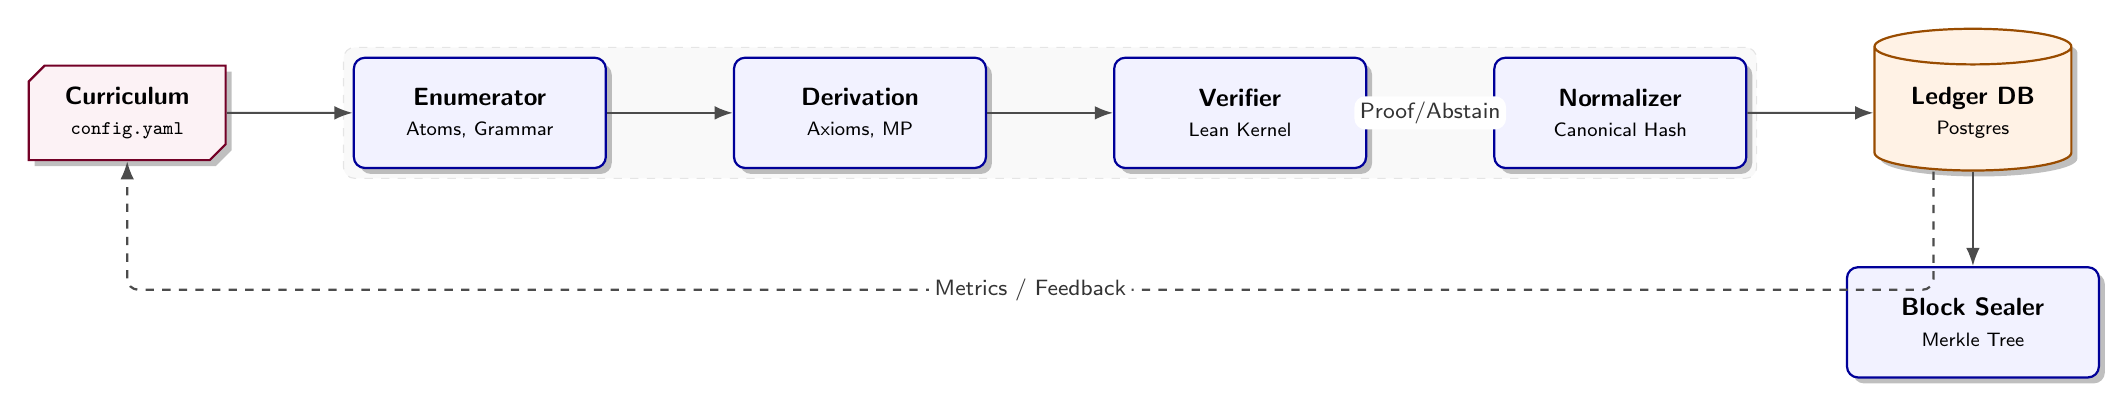
\begin{tikzpicture}[node distance=1.2cm and 1.6cm]
  % Nodes
  \node[config] (yaml) {\textbf{Curriculum}\\\scriptsize \texttt{config.yaml}};
  \node[process, right=of yaml] (enum) {\textbf{Enumerator}\\\scriptsize Atoms, Grammar};
  \node[process, right=of enum] (derive) {\textbf{Derivation}\\\scriptsize Axioms, MP};
  \node[process, right=of derive] (lean) {\textbf{Verifier}\\\scriptsize Lean Kernel};
  \node[process, right=of lean] (canon) {\textbf{Normalizer}\\\scriptsize Canonical Hash};
  \node[datastore, right=of canon] (db) {\textbf{Ledger DB}\\\scriptsize Postgres};
  \node[process, below=of db] (blocks) {\textbf{Block Sealer}\\\scriptsize Merkle Tree};

  % Edges
  \draw[line] (yaml) -- (enum);
  \draw[line] (enum) -- (derive);
  \draw[line] (derive) -- (lean);
  \draw[line] (lean) -- node[label_text]{Proof/Abstain} (canon);
  \draw[line] (canon) -- (db);
  \draw[line] (db) -- (blocks);

  % Feedback Loop
  \draw[line, dashed] (db.south) ++(-0.5,0) coordinate(dbs) -- ++(0,-1.5) -| (yaml.south) node[pos=0.25, label_text, fill=white] {Metrics / Feedback};
  
  % Background
  \begin{scope}[on background layer]
    \node[fit=(enum)(derive)(lean)(canon), rounded corners, fill=gray!5, draw=gray!20, dashed] {};
  \end{scope}
\end{tikzpicture}
\caption{Core Pipeline: From curriculum parameters to immutable ledger blocks.}
\end{figure}

\subsection{Data Model Intuition}

The core tables (conceptually):
\begin{itemize}[leftmargin=1.5em]
  \item \texttt{statements}: logical formulas, normalized, with $\hash(s)$ as primary identity.
  \item \texttt{proofs}: proof objects with fields such as prover, method, duration, status, transcript hash.
  \item \texttt{dependencies}: edges in the proof DAG (which proof depends on which statements).
  \item \texttt{blocks}: batches of proofs, with Merkle roots $R_t$.
  \item \texttt{runs}: operational metadata per run of the derivation engine / RFL.
\end{itemize}

Your mental model: the ledger is a big, append-only DAG of reasoning, with blocks providing cryptographic checkpoints.

\subsection*{Addendum: Topological Structure of Proof DAGs}
\addcontentsline{toc}{subsection}{Addendum: Topological Structure of Proof DAGs}

The global proof DAG maintained by \system{} is not merely a dependency graph; it is a
\emph{topological object}. Many structural properties of the organism---lemma reuse,
concept emergence, proof-strategy divergence, and reasoning degeneracy---manifest as
changes in the topology of local subgraphs.

In preparation for Phase~III, each local proof DAG $G=(V,E)$ can be lifted to a
\emph{simplicial complex} $K_{\mathrm{comb}}$ (a flag complex), by treating cliques in the
undirected 1-skeleton of $G$ as simplices. Cycles in $H_1(K_{\mathrm{comb}})$ correspond to
nontrivial reuse patterns or logical ``loops''; fragmentation in $H_0$ indicates instability
or degeneracy in reasoning. These constructions power the TDA Mind Scanner defined in
Appendix~C.

In short: the DAG is the ``visible anatomy,'' but its simplicial complex is the
``structural geometry.'' Both will be essential for understanding drift, stability, and
emergent behavior as RFL scales.

% ============================================================
\section{The Logic Ladder and Curriculum Slices}
\label{sec:curriculum}

\subsection{Curriculum as a Control Surface}

The curriculum ladder formalizes how the system climbs from simple theories to more complex ones.

At the bottom: propositional logic (PL). Above: FOL with equality, equational theories, linear arithmetic.

Each rung is not a monolithic theory, but a set of \emph{slices}:
bounded combinations of atom counts, formula depth, search budgets, etc.

\begin{definition}[Slice]
A \emph{slice} is a tuple of parameters:
\[
  (\text{atoms}, \text{depth}, \text{breadth}, \text{total}, \text{timeout}, \dots)
\]
governing enumeration and derivation for a constrained subspace of formulas.
\end{definition}

The curriculum specifies:
\begin{itemize}[leftmargin=1.5em]
  \item which slices exist per theory;
  \item what coverage / throughput / abstention thresholds they must meet before the system is allowed to ratchet upward.
\end{itemize}

\subsection{Authentic Synthetic Data}

Rather than scraping human-written proofs from the internet, \system{} generates its own statements within these slices and proves them (or abstains). This yields:
\begin{itemize}[leftmargin=1.5em]
  \item infinite data (the space of formulas grows combinatorially),
  \item with perfect provenance (every statement has a known hash and proof path),
  \item and tunable difficulty (via slice parameters).
\end{itemize}

For your purposes: the ladder is the "training curriculum" for the organism.

% ============================================================
\subsection{LeCun's Grounding Critique and the Role of Authentic Synthetic Data}
\label{subsec:lecun-grounding-authentic-synth}

This manual distinguishes two different notions of ``grounding'' that are often conflated in contemporary debates about large language models (LLMs).

\paragraph{(1) Physical / sensorimotor grounding.}
This is the grounding Yann LeCun emphasizes: continuous, embodied, action-conditioned experience (objects, gravity, contact dynamics, causality in time). Under this framing, token prediction alone is an insufficient route to robust world models. This diagnosis is broadly correct and does not conflict with \system{}'s design goals.

\paragraph{(2) Epistemic / truth grounding.}
This is the grounding problem \system{} targets: whether a system's outputs are warranted (provable, checkable, auditable), whether it can abstain rather than bluff, and whether its learning dynamics remain stable under feedback. Hallucination is primarily an \emph{epistemic discipline} failure, not a sensorimotor failure.

\paragraph{Authentic synthetic data is epistemic grounding, not physical grounding.}
\system{} does not claim to replace embodiment, simulate physics in prose, or solve commonsense perception. Instead, \emph{authentic synthetic data} is defined as:
\begin{quote}
\emph{Synthetic data generated within a rule-governed micro-world, whose labels and outcomes are externally enforced by an oracle (e.g., a proof kernel), with full provenance and replayability.}
\end{quote}

In the propositional and formal reasoning regimes, the ``micro-world'' is the formal system itself; the oracle is the verifier ladder (Lean / proof-or-abstain). This yields a feedback loop with real consequence:
\[
\text{attempt} \;\to\; \text{verify/reject/abstain} \;\to\; \text{attest} \;\to\; \text{update}.
\]

\paragraph{Why this matters for compute-vs-data bottlenecks.}
LeCun's ``compute will always be the bottleneck'' intuition is strongest when the only path to grounding is high-bandwidth raw sensory streams. \system{} exploits a different asymmetry:
\begin{itemize}[leftmargin=1.5em]
  \item the data space is combinatorial (generated, not scraped),
  \item feedback is objective and cheap (kernel accept/reject/abstain),
  \item errors are catastrophic and detectable (no soft correctness),
  \item provenance is exact (hash + proof path),
  \item curriculum difficulty is controllable (slices and ratchets).
\end{itemize}
In this regime, the dominant bottlenecks are not ``more pixels'' or ``more tokens'' but rather search strategy, curriculum design, stability of updates, and governance of learning dynamics.

\paragraph{The neuro-symbolic flywheel and the trust bottleneck.}
The intended neuro-symbolic flywheel is:
\[
\text{model proposes} \;\to\; \text{verifier enforces truth} \;\to\; \text{ledger records only attested outcomes} \;\to\; \text{RFL updates from verified signals}.
\]
This directly targets hallucination by enforcing (i) proof-or-abstain at production time, (ii) verifier-gated learning signals at update time, and (iii) a monotone, provenance-preserving memory substrate (the ledger) over time.

\paragraph{Honest status: Phase I substrate vs Phase II flywheel.}
Phase~I establishes the governance substrate required for trustworthy flywheel operation: dual attestation, claim discipline, determinism, signed evidence artifacts, and SHADOW-mode semantics. The full capability ladder execution---continuous autonomous curriculum ascent producing large volumes of authentic synthetic data---is a Phase~II execution objective. This separation is intentional:
\begin{quote}
\emph{The flywheel should not be turned on before the substrate can prevent epistemic decay.}
\end{quote}

\noindent\textit{SHADOW-OBSERVE --- verification results are non-blocking.}

% ============================================================
\subsection{Authentic Synthetic Data as Policy-Evolution Evidence}
\label{subsec:authentic-synth-policy}

This manual uses the phrase \emph{authentic synthetic data} in a deliberately nonstandard way.
The term does \emph{not} refer to conventional model training corpora (next-token pretraining,
instruction tuning, or ``LLM teaches itself facts''). In \system{}, the primary synthetic
asset is not content, but \emph{policy-evolution evidence}.

\paragraph{Definition (operational).}
An authentic synthetic record is an attested event of the form:
\[
\langle \text{regime},\ \text{verifier},\ \text{constraints},\ \mathcal{V}(e)\in\{1,0,\bot\},\ \Delta\pi\ \rangle,
\]
where $\mathcal{V}(e)$ is a fail-closed outcome (verified / refuted / abstained) produced under a
declared verification boundary, and $\Delta\pi$ denotes an admissible (possibly zero) governance-policy
update derived from that outcome. The record is valuable precisely because it binds:
(i) a bounded epistemic regime, (ii) a replayable outcome, and (iii) an update eligibility decision
into a single auditable artifact.

\paragraph{Consequence.}
The synthetic stream therefore teaches the system \emph{how epistemic authority may move} under
evidence, not \emph{what to say}. This is why ``policy'' matters more than ``model'' in the Phase~I
story: the data are calibration traces for governance dynamics.

% ============================================================
\subsection{Why the Capability Ladder Is Not Discarded}
\label{subsec:why-not-kick-ladder}

A natural temptation is to treat the capability ladder as scaffolding: once a policy appears to
stabilize, one might ask why not ``kick the ladder away.'' This is a subtle but dangerous category
error. Empirical stability along many training paths suggests \emph{path robustness}, not
\emph{path independence}. The ladder may lead to similar policy geometry across many trajectories,
but it does not thereby become irrelevant.

\paragraph{The ladder is a calibration instrument, not training wheels.}
The capability ladder does not exist primarily to ``teach answers.'' It exists to provide a
permanent, replayable calibration environment in which truth-conditional outcomes are available and
failure modes are unambiguous. Its role after apparent convergence is to remain a live reference:
a reference clock, a unit standard, or a regression test suite for epistemic behavior.

\paragraph{Why the reference must remain live.}
Once the system operates in partially verifiable or human-attested regimes, the learning signal
becomes noisier and more adversarial. Without an always-available calibration environment, the
system loses its ability to distinguish:
\begin{quote}
\emph{``the world changed''} \quad\text{from}\quad \emph{``the policy drifted because the signal degraded.''}
\end{quote}
Keeping the ladder available preserves observability, drift detectability, and rollback discipline.

\paragraph{Open-endedness is structural.}
Even in mathematics, novelty and uncertainty are inexhaustible (Gödel-style incompleteness is one
expression of this fact). The ladder is therefore not a finite staircase to be ``completed,'' but a
growing family of verifiable calibration regimes. \system{} does not graduate from calibration; it
preserves calibration as the mechanism that prevents epistemic self-corruption as domains become
less decidable.

% ============================================================
\subsection{Calibration Environments and Collapse Diagnostics}
\label{subsec:calibration-and-collapse}

\system{} treats \emph{calibration} as a first-class governance primitive: whenever possible, policy update dynamics are anchored to regimes where error is externally checkable and failure modes are typed (e.g., \texttt{VERIFIED}/\texttt{REFUTED}/\texttt{ABSTAINED}) rather than silently absorbed. This motivates designing \emph{wind-tunnel} evaluation environments: controlled tasks where the relevant ground truth is known (or mechanically checkable) and memorization or informal attribution is ruled out.

\paragraph{Bayesian wind tunnels.}
Recent work on Bayesian wind tunnels provides a concrete template: construct settings in which the analytic posterior is known in closed form and memorization is provably infeasible, converting qualitative claims (``does the model do Bayes?'') into quantitative calibration tests (e.g., posterior-entropy tracking error measured in bits). In such regimes, architecture-level mechanisms can be isolated and audited, and calibration error becomes a ledgerable scalar diagnostic rather than a narrative claim.

\paragraph{Representational alignment and collapse.}
A complementary diagnostic arises from representational analysis across independently trained models. Evidence from scientific foundation models suggests that (i) high-performing models trained on similar regimes can exhibit strong \emph{representational alignment} despite architectural and modality differences, while (ii) out-of-distribution inputs can induce \emph{representation collapse} onto low-information, architecture-dominated manifolds. For \system{}, this supports a governance rule-of-thumb: when external diagnostics indicate collapse (e.g., sharply reduced representational alignment or other low-information signatures), downstream influence should be downgraded (stricter trust class, increased abstention, or mandatory reformulation / stronger verification), rather than compensated by higher confidence.

\paragraph{Collapse--Equilibrium Indistinguishability.}
In regimes lacking external verification, apparent convergence of internal representations (e.g., agreement across models or collapse to low-dimensional manifolds) is epistemically ambiguous: such behavior may reflect either a genuine invariant or a low-information inductive-bias sink. Because these cases are observationally indistinguishable without external checks, \system{} treats them uniformly as epistemically degraded regimes. Convergence alone never upgrades trust or confidence; instead, it triggers conservative routing (trust-class downgrade, increased abstention, reformulation, or escalation to stronger verification). This design prevents consensus or representational agreement from being Goodharted into unwarranted authority.

\paragraph{Curriculum scope discipline.}
Evidence from human and transformer learning indicates that data distributional properties can systematically trade off between ``in-context'' generalization and ``in-weights'' memorization, and that curriculum schedules that benefit humans do not necessarily benefit transformer networks in the same way. This motivates explicitly scoping curriculum claims: in \system{}, curricula are always appropriate for \emph{human internalization and governance workflows}, but claims about curricula improving model weights must be treated as empirical and fragment-scoped. In particular, redundancy/diversity mix should be treated as a governed configuration variable when generating authentic synthetic data streams for policy calibration.

\paragraph{Design implication.}
The ladder is not only a progression of expressive fragments; it is also a bank of calibration environments and collapse diagnostics. Where verification is available, it dominates. Where it is not, policy should remain constrained by diagnostics learned under verifiable pressure, and collapse signatures should trigger conservative routing rather than confident extrapolation.

% ============================================================
\subsection{Capability Ladder Discipline: When to Move Up a Rung}
\label{subsec:ladder-discipline}

A recurring failure mode in the broader ``AI reasoning'' ecosystem is \emph{silent capability creep}:
systems acquire new inference power (heuristics, solver delegation, unbounded generalization, or implicit
assumption broadening) without an explicit, auditable transition.
\system{} treats this as a governance defect.

\paragraph{Rungs are sealed fragments, not vague milestones.}
A ``rung'' in the \system{} ladder is not defined by ``how many truths were proven'' (which is not a meaningful
completion criterion in an open-ended logic). Instead, a rung is a \emph{versioned, bounded logic fragment}
whose semantics and failure behavior are fully specified and testable. For example, \texttt{FOL\_FIN\_EQ\_v1}
is intentionally \emph{not} ``full FOL='' or general theorem proving. It is a fenced fragment: finite domains
only, equality only, functions given by total/closed tables, \emph{no predicates}, and verification by
\emph{exhaustive enumeration only}.

\paragraph{What ``we can prove we did not move there'' means.}
The phrase ``we can prove, cryptographically, that we have not moved there yet'' refers to preventing
non-audited transition into \emph{unbounded reasoning power} (e.g., infinite domains, Skolemization,
SMT/SAT delegation, heuristic proof search, learned inference shortcuts, or silent generalization).
\system{} enforces this boundary mechanically:
\begin{itemize}[leftmargin=1.5em]
  \item \textbf{Fragment identity locks:} artifacts are stamped with a \texttt{logic\_fragment} identifier and
        \texttt{verification\_strategy} (e.g., \texttt{FOL\_FIN\_EQ\_v1} and \texttt{exhaustive\_enumeration}).
        Mismatches are treated as invalid.
  \item \textbf{Fail-closed resource bounds:} when a query exceeds declared limits (domain size, quantifier depth,
        or assignment bound), the system must abstain rather than improvise.
  \item \textbf{Golden-hash closure:} deterministic evidence packs provide a ``no silent drift'' alarm. Any change
        to semantics, enumeration order, certificate structure, or admissibility rules becomes a versioned break
        (and therefore cannot occur invisibly).
\end{itemize}

\paragraph{Promotion criteria: closure first, then expressivity.}
\system{} does not ``move up'' when the ledger contains ``enough'' statements. Instead, promotion is authorized only when:
\begin{enumerate}[leftmargin=1.5em]
  \item \textbf{Rung closure:} semantics are fully specified; failure modes are enumerated; outputs are auditable;
        determinism is demonstrated; and silent extension is structurally impossible.
  \item \textbf{Behavioral uplift without semantic mutation:} reflexive updates (RFL) improve epistemic posture
        (e.g., fewer unjustified abstentions, earlier counterexample detection) under frozen semantics.
  \item \textbf{Stability under pressure:} governance updates do not oscillate or expand expressivity; they remain
        within the declared admissibility envelope.
\end{enumerate}

\paragraph{The core inversion.}
The intended sequencing is:
\begin{quote}
\emph{Policy discipline climbs first; logical expressivity climbs last.}
\end{quote}
This inversion is deliberate: it ensures the system can demonstrably survive \emph{not knowing} (abstention,
negative knowledge, fail-closed behavior) before it acquires more powerful inference machinery.

% ============================================================
\subsection{Execution Phase: The Human Checksum}
\label{subsec:human-checksum}

Once a rung is sealed, the primary bottleneck is no longer engineering novelty but \emph{deployment-grade articulation}.
At acquisition time, the system must be defensible under adversarial questioning:
what it does, what it explicitly does not do, why it fails closed, and how the absence of silent drift is verified.
Accordingly, after sealing a fragment, the correct operational posture is:
\begin{itemize}[leftmargin=1.5em]
  \item freeze features (avoid ``helpful'' refactors that change semantics),
  \item drill concise explanations (60-second and 5-minute versions with explicit non-claims),
  \item use adversarial review to identify ambiguity before external stakeholders do,
  \item perform measured outreach (few high-integrity conversations rather than broad marketing).
\end{itemize}
In this phase, the system artifacts speak for themselves; the remaining requirement is a human operator who can
match the system's precision and scope discipline in live technical conversation.

% ============================================================
\section{Dual Attestation and User-Verified Input}
\label{sec:dual-attestation}

\subsection{Reasoning Root and UI Root}

The ledger attests to the machine’s reasoning via $R_t$; the UI layer attests to human interaction via $U_t$.

\begin{definition}[Dual Attestation]
Let $R_t$ be the Merkle root over proof IDs in block $t$ (reasoning stream). Let $U_t$ be the Merkle root over UI events in the same epoch (user stream). Define the composite root:
\[
  H_t = \Hash(\texttt{"EPOCH:"}\concat R_t \concat U_t),
\]
binding what was \emph{thought} to what was \emph{asked/confirmed}.
\end{definition}

This is the basis of the \emph{Chain of Verifiable Cognition}:
every epoch $t$ has a cryptographic fingerprint $H_t$ that commits to both reasoning and UI.

Conceptually, within an epoch you may also track per-step roots (for fine-grained audit):
\begin{itemize}[leftmargin=1.5em]
  \item $r_\tau$: Merkle root over reasoning events at time-step $\tau$;
  \item $u_\tau$: Merkle root over UI events at time-step $\tau$;
  \item these feed into $R_t$ and $U_t$ via higher-level Merkle constructions.
\end{itemize}

\subsection{User-Verified Input Loop (UVIL)}

The UI is not just a front-end; it is part of the epistemic circuit.

\begin{definition}[User-Verified Input Loop]
Each user interaction is encoded as an event
\[
  \tau = \langle \texttt{actor},\ \texttt{kind}\in\{\text{confirm},\text{correct},\text{abstain}\},\ \texttt{target\_hash},\ \texttt{meta} \rangle
\]
and enters the UI-Merkle structure. The UVIL is the process by which these events are:
\begin{enumerate}[leftmargin=1.5em]
  \item normalized and recorded;
  \item referenced by $U_t$ and hence by $H_t$;
  \item later available as evidence in RFL updates and audits.
\end{enumerate}
\end{definition}

The key concept: human judgment is not "soft feedback"; it becomes a first-class, cryptographically-attested part of the substrate.

% ============================================================
\subsection{Authority Binding: What Humans Retain (and What They Do Not)}
\label{subsec:authority-binding}

A subtle but dangerous ambiguity in human-in-the-loop AI systems is whether the human is being asked to \emph{judge correctness} of model reasoning. \system{} explicitly rejects that framing.

\paragraph{Humans do not replace the verifier.}
Humans (or institutions) are not the epistemic authority for formally verifiable claims. Correctness is decided by the strongest applicable external regime (e.g.\ Lean for formal mathematics). Human involvement is not a substitute for verification.

\paragraph{Humans bind authority, not truth.}
The role of User-Verified Input (UVIL) is \emph{authority binding}:
a deliberate, auditable act by which a human or institution commits that a particular artifact (and its trust class) may influence future cognition \emph{in this context}, or that abstention is the correct outcome.

Concretely, UVIL events encode that humans retain authority over:
\begin{itemize}[leftmargin=1.5em]
  \item \textbf{when proof is demanded} (escalate to a stronger regime vs remain advisory),
  \item \textbf{what trust class applies} (FV/MV/PA/ADV) and the scope of that classification,
  \item \textbf{when abstention is correct} (refuse claim escalation under uncertainty),
  \item \textbf{which claims may influence future cognition} (admissible vs inert).
\end{itemize}

\paragraph{Resolution of the ``replacement'' confusion.}
\system{} is not attempting to replace human judgment with model judgment.
It binds human (or institutional) authority into the substrate so that epistemic scope, consent, and responsibility are explicit and replayable rather than implicit and deniable.

\subsection{Human Roles Under Autonomy: Cognition vs Sovereignty}
\label{subsec:human-roles-autonomy}

A persistent confusion in AI safety discourse conflates two distinct human functions:
\begin{enumerate}[leftmargin=1.5em]
  \item \textbf{Cognitive engine:} Human as the source of reasoning, judgment, or correctness evaluation.
  \item \textbf{Sovereign boundary-setter:} Human as the authority that defines what kinds of cognition are admissible.
\end{enumerate}

\paragraph{Why the distinction matters.}
As AI systems scale, using humans as cognitive engines becomes untenable:
\begin{itemize}[leftmargin=1.5em]
  \item Human throughput does not scale with model inference speed.
  \item Human correctness judgment on formal domains is often inferior to machine verification.
  \item Requiring human review of every reasoning step creates bottlenecks that defeat automation benefits.
\end{itemize}

Conversely, using humans as sovereign boundary-setters \emph{always} scales:
\begin{itemize}[leftmargin=1.5em]
  \item Boundary decisions are infrequent (policy changes, not per-inference).
  \item Authority binding is a one-time commitment, not continuous labor.
  \item Governance constraints propagate automatically once encoded.
\end{itemize}

\paragraph{\system{} operationalizes this distinction.}
The User-Verified Input Loop (UVIL) is explicitly \emph{not} a mechanism for humans to judge correctness. It is a mechanism for humans to:
\begin{itemize}[leftmargin=1.5em]
  \item declare which trust classes apply to which contexts,
  \item commit that certain artifacts may influence future cognition,
  \item escalate or de-escalate verification requirements,
  \item authorize or forbid specific learning trajectories.
\end{itemize}

\paragraph{Implication for autonomy.}
Under this framing, increased autonomy does not mean ``humans do less.'' It means humans shift from cognitive labor (which doesn't scale) to sovereignty exercise (which must remain human). The more autonomous the system, the more critical it becomes that boundary-setting authority is explicit, auditable, and non-delegable.

% ============================================================
\section{Trust Classes and Cryptographic Commitment}
\label{sec:trust-classes}

MathLedger does not attempt to collapse all forms of correctness, validation, or judgment into a single notion of ``truth.'' Instead, it explicitly distinguishes \emph{trust classes}: categories of artifacts differentiated by the strongest verification mechanism applicable to them.

This distinction is not cosmetic. It is fundamental to governance, auditability, and long-term system integrity.

\subsection{Trust Classes}

Each artifact recorded by MathLedger belongs to exactly one trust class:

\begin{itemize}
  \item \textbf{Formally Verified}: Artifacts whose correctness is established by a small, trusted kernel (e.g., Lean). These include formal statements and proof objects.
  \item \textbf{Mechanically Validated}: Artifacts whose correctness can be established by deterministic computation, tests, or certificates (e.g., recomputation, constraint checking).
  \item \textbf{Procedurally Attested}: Artifacts whose trust derives from provenance, authorization, or process (e.g., who approved what, under which authority).
  \item \textbf{Advisory}: Interpretive or heuristic outputs (e.g., narrative analyses, recommendations) that are explicitly not formally or mechanically verified.
\end{itemize}

These trust classes are intentionally non-interchangeable. A formally verified artifact is not ``more correct'' in a metaphysical sense; it is correct in a strictly narrower, explicitly defined domain.

\subsection{Separation of Verification and Attestation}

MathLedger enforces a strict separation between:
\begin{itemize}
  \item \emph{Verification} (establishing correctness relative to a formal system or checker), and
  \item \emph{Attestation} (recording intent, context, and provenance).
\end{itemize}

This separation prevents category errors such as treating interpretive judgments as formal truths or retroactively upgrading the trust status of an artifact.

\subsection{Cryptographic Commitment to Trust Class}

To prevent post hoc relabeling or misrepresentation, each artifact's trust class is included in the canonical serialization that is hashed into the ledger.

Concretely, each Merkle leaf commits to:
\[
\Hash(\texttt{trust\_class} \concat \texttt{artifact\_kind} \concat \texttt{artifact\_digest} \concat \texttt{checker\_id} \concat \texttt{checker\_version} \concat \ldots)
\]

This ensures that:
\begin{itemize}
  \item trust class is immutable once recorded,
  \item cryptographic integrity binds verification level to artifact content,
  \item future auditors cannot reinterpret an artifact under a stronger trust class than originally justified.
\end{itemize}

\subsection{Trust Monotonicity: Preventing Truth Laundering}
\label{subsec:trust-monotonicity}

A central failure mode of contemporary language-model systems is \emph{truth laundering}:
an output that is merely heuristic (a guess, a plausible explanation, a narrative) is presented
with the rhetorical posture of a verified fact. \system{} is designed to prevent this
category error \emph{structurally}, not by asking the model to be honest.

\paragraph{Typed trust.}
Every artifact is assigned a \emph{trust class} at creation time, and the trust class is
cryptographically committed as part of the artifact identity. Concretely, each Merkle leaf
commits to the tuple
\[
\Hash\!\left(
\texttt{trust\_class} \concat
\texttt{artifact\_kind} \concat
\texttt{artifact\_digest} \concat
\texttt{checker\_id} \concat
\texttt{checker\_version} \concat
\texttt{schema\_version}
\right),
\]
so the system cannot retroactively reinterpret an advisory artifact as formally verified,
and a downstream consumer cannot ``forget'' which authority (if any) was applied.

\paragraph{Monotonicity invariant.}
\system{} enforces a simple but powerful rule:

\begin{quote}
\emph{Trust is monotone: an artifact cannot move from a weaker trust class to a stronger
trust class without a new external verification event producing a new canonical artifact.}
\end{quote}

This monotonicity is the formal counterpart of ``true or silent.'' The system does not
force correctness in domains where correctness cannot be mechanically established; instead,
it forces \emph{epistemic honesty}: any output that is not backed by an applicable external
authority remains explicitly low-trust.

\paragraph{Operational meaning of ``true or silent.''}
In \system{}, ``silence'' is not the absence of text. It is the absence of authority.
Control-plane gates and high-stakes workflows are configured to consume only selected
trust classes (e.g.\ \textbf{Formally Verified} or \textbf{Mechanically Validated}).
Artifacts in \textbf{Advisory} class may still exist and be recorded, but they are treated
as non-authoritative and may be ignored by default in safety-critical pathways.

\paragraph{Boundary of the claim.}
This mechanism should be understood precisely:

\begin{itemize}[leftmargin=1.5em]
  \item \textbf{Not claimed:} ``\system{} guarantees truth in the real world'' or ``the agent cannot output false statements.''
  \item \textbf{Claimed:} unverified outputs cannot silently accumulate into verified authority; uncertainty cannot be concealed by rhetorical confidence; and any upgrade in epistemic status must occur via an explicit, auditable verification pathway.
\end{itemize}

In short: \system{} does not make systems truthful by optimism; it makes them \emph{unable to
misrepresent their epistemic status} without detection.

% ============================================================
\subsection{Trust Classes and UVIL Are Complementary}
\label{subsec:trust-uvil-complement}

Trust classes and UVIL answer different questions and therefore do not conflict.

\paragraph{Trust classes (typing).}
A trust class records the strongest verification regime an artifact actually satisfies (FV/MV/PA/ADV). This classification is cryptographically committed, non-upgradable, and prevents truth laundering.

\paragraph{UVIL (authority binding).}
UVIL records whether a human or institution \emph{binds authority} to a specific artifact \emph{in a specific context}---e.g.\ whether it may influence durable policy, memory consolidation, curriculum progression, or claim escalation.

\paragraph{No ``upgrade'' power.}
UVIL cannot upgrade an artifact's trust class. A human can authorize \emph{use within the class}, or refuse authorization (including selecting abstention), but cannot elevate an advisory artifact into a formally verified one without an actual external verification event producing a new artifact.

\paragraph{Operational pattern: AI proposes, humans ratify.}
In practice, \system{} is designed for expert operator workflows (research, audit, deployment), not mass consumer epistemology. A scalable interaction pattern is:
\begin{enumerate}[leftmargin=1.5em]
  \item \textbf{AI proposes} a candidate artifact together with a suggested trust class and scope.
  \item \textbf{Humans (or institutions) ratify} (confirm/correct/abstain) via UVIL, producing a committed UI event.
  \item \textbf{RFL admissibility} consumes only those events authorized under the declared trust class and scope.
\end{enumerate}

This matches modern ``coding agent'' workflows (proposal $\rightarrow$ review $\rightarrow$ commit), while preserving epistemic discipline.

% ============================================================
\subsection{Capability Ladder vs.\ Governance: Expressivity and Influence Are Orthogonal}
\label{subsec:ladder-vs-governance-orthogonal}

The capability ladder and the governance substrate answer different questions and must not be conflated.

\paragraph{Capability ladder (expressivity).}
Each rung specifies what kinds of statements the verifier can even represent and check (e.g.\ PL vs.\ finite-domain FOL fragments).
This is object-level expressive power: \emph{what can be said and proved} in a given formal regime.

\paragraph{Governance substrate (influence).}
\system{} governs a different axis: \emph{what is allowed to matter}.
It constrains learning authority, claim escalation, and durable memory by enforcing determinism, replayability, typed outcomes, and fail-closed admissibility.
These invariants are designed to survive verifier upgrades: changing the verifier changes what can be checked, not how authority is granted.

\paragraph{Trust classes cut across the ladder.}
Trust classes do not arrive ``after'' the ladder; they partition influence \emph{across} all rungs.
They answer: even if a claim is true in logic $L$, is it permitted to influence policy, memory, or action in this context?
This is a control-plane question, not a logic question.

\paragraph{Transcendence as demotion of the ladder.}
As expressivity increases, the ladder becomes an input stream among others rather than the source of authority.
The governance substrate does not supersede the ladder; it demotes the ladder from \emph{authority} to \emph{evidence}.
This is the correct ordering:

\begin{quote}
\emph{The ladder governs expressivity. \system{} governs influence. Trust classes partition influence when expressivity outpaces safety.}
\end{quote}

\subsection{Negative Knowledge and Frozen Governance Commitments}
\label{subsec:negative-knowledge-frozen-commitments}

\system{} treats failure traces as first-class governance artifacts. Beyond recording verifier-accepted outcomes, the substrate can also cryptographically seal \emph{negative knowledge}: refutations, counterexamples, UNSAT certificates, and explicitly inadmissible update attempts (e.g., governance-trigger events). These artifacts are recorded with the same provenance discipline as successes (canonical identity, deterministic serialization, and replayable evidence) and are intended for third-party audit rather than model performance optimization.

This matters because post-hoc safety and compliance regimes often require not only evidence of what succeeded, but evidence of what was rejected and why. Attested refutations provide a conservative, replayable map of inadmissible regions of behavior: they do not assert capability, but they do preserve audit-grade warnings that can be independently re-verified. In this sense, replay in \system{} is evidentiary rather than heuristic.

In addition, \system{} allows experiments to bind themselves to a versioned set of \emph{frozen governance commitments}: non-negotiable constraints that are declared, hashed, and enforced as out-of-band admissibility requirements. Concretely, an execution may commit to a Governance Commitment Registry (GCR) whose identifier (and enforcement-code version) is recorded in the run provenance. These commitments are not treated as mathematical axioms inside the proof kernel; rather, they gate claim escalation and learning updates under a fail-closed policy. This provides a simple audit primitive: a third party can verify that a run was executed under commitments $C$ and that violations were treated as inadmissible.

% ============================================================
\subsection{Governance Commitment Sets as First-Class Artifacts}
\label{subsec:policy-as-artifact}

\paragraph{Non-mutable policy.}
\system{} does not treat governance policy as mutable configuration. Governance exists only as
versioned, hash-addressed commitment artifacts. Policy evolution therefore occurs only by producing
new commitment artifacts, never by mutating an existing policy in place.

\paragraph{Commitment registry root (policy Merkle root).}
Let $G_t = \{g_1,\dots,g_n\}$ be the set of active governance commitment artifacts at epoch $t$.
Each $g_i$ has a canonical encoding and a content hash $\Hash(g_i)$. The authoritative governance state
is committed via a Merkle root:
\[
  R^{\mathrm{gcr}}_t \;=\; \mathrm{MerkleRoot}\bigl(\Hash(g_1),\dots,\Hash(g_n)\bigr).
\]
This root functions as a cryptographic commitment to ``the full set of policies in force.''

\paragraph{Binding artifacts to governance state (non-retroactivity).}
Each authority-bearing artifact produced at epoch $t$ must carry (directly or via the manifest) the
identifier of the active governance commitment root $R^{\mathrm{gcr}}_t$. This ensures:
\begin{itemize}[leftmargin=1.5em]
  \item an artifact can be audited relative to the exact rules under which it was admissible;
  \item later governance changes do not retroactively reinterpret earlier artifacts;
  \item policy evolution remains explicit and replay-verifiable.
\end{itemize}

\paragraph{Dual attestation is distinct.}
Policy Merkle commitments should not be conflated with dual attestation. Dual attestation binds
reasoning artifacts ($R_t$) to the UI event stream ($U_t$) into an epoch fingerprint $H_t$:
\[
  H_t \;=\; \Hash\!\bigl(\texttt{"EPOCH:"}\concat R_t \concat U_t\bigr).
\]
This answers ``what was proven/recorded and what was asked/confirmed.'' The governance commitment root
$R^{\mathrm{gcr}}_t$ answers ``under which rules was authority permitted.'' They are complementary and
should remain separately versioned and auditable.

% ============================================================
\subsection{Epistemic Irreversibility and One-Way Doors}
\label{subsec:epistemic-irreversibility}

A central design objective of \system{} is not raw optimization power but \emph{epistemic irreversibility}:
the system should contain explicit, auditable ``one-way doors'' that prevent authority from drifting
silently over time.

\paragraph{Why irreversibility matters.}
Many AI governance failures are epistemically reversible:
logs can be reinterpreted, scopes can be retroactively expanded, metrics can be reframed, and
learning can occur through untyped channels. When audit narratives are reversible, trust collapses
under adversarial scrutiny.

\paragraph{Irreversibility primitives in \system{}.}
\system{} introduces irreversible commitments of the following forms:
\begin{itemize}[leftmargin=1.5em]
  \item \textbf{Non-upgradable trust typing:} once an artifact is committed under a trust class, it cannot be silently upgraded to a stronger class without a new external verification event producing a new artifact identity.
  \item \textbf{Run-bounded governance:} execution is bound to a versioned, hash-committed governance registry; a run cannot be retroactively ``re-scoped'' without producing a new, auditable run record.
  \item \textbf{Provable non-learning:} blocked or inadmissible update attempts are recorded as typed, replayable artifacts; absence of admissible learning is itself an auditable state.
  \item \textbf{Fail-closed replay:} verification fails closed on missing fields, invalid enums, or hash mismatches, preventing ``papered-over'' compliance narratives.
\end{itemize}

\paragraph{Design consequence.}
\system{} enforces that \emph{history matters} in cognition: authority cannot creep, and governance
cannot be rewritten by competence. This is intentionally conservative: false negatives are acceptable;
false positives (unverified authority) are catastrophic.

\subsection{Contextual Incompatibilities (Without Global Contradiction)}
\label{subsec:contextual-incompatibilities}

Classical proof systems treat global contradictions as catastrophic (principle of explosion). Accordingly, \system{} does not elevate $P \wedge \neg P$ to a global truth claim. Instead, when two propositions are individually verified under distinct assumption contexts but cannot be jointly satisfied under a unified context (or under the active commitment registry), \system{} records this as a \emph{contextual incompatibility artifact}. A minimal form is:
\[
\mathcal{C}_A \vdash P,\quad \mathcal{C}_B \vdash Q,\quad \mathrm{UNIFY}(\mathcal{C}_A,\mathcal{C}_B)\;\Rightarrow\;\mathrm{UNSAT}
\]
(or a registry violation), together with the corresponding proof/certificate objects. This preserves audit-grade ``negative space''---documented incompatibilities that constrain admissible updates---without adopting paraconsistent logic or weakening kernel soundness.

% ============================================================
\subsection{Intelligence, Knowledge, and Governance}
\label{subsec:intelligence-knowledge-governance}

\paragraph{Distinction.}
\system{} separates three concepts that are often conflated:
\begin{itemize}[leftmargin=1.5em]
  \item \textbf{Intelligence:} capacity to generate predictions, plans, and candidate claims.
  \item \textbf{Knowledge:} the subset of claims that are justified, stabilized, and permitted to carry authority.
  \item \textbf{Governance:} the rules that determine what may count as knowledge and what may influence future cognition.
\end{itemize}

\paragraph{Core stance.}
Intelligence may scale rapidly. Knowledge need not.
\system{} allows unlimited generation of candidate artifacts while refusing to let untyped or
unverified artifacts silently harden into authority. This is epistemic hygiene, not censorship.

\subsection{Graduated Verifiability and Epistemic Stratification}
\label{subsec:graduated-verifiability}

\paragraph{Non-Goal: Universal Verification.}
\system{} does not aim to ``verify natural language'' in a uniform or total sense.
The question ``Can language be verified like mathematics?'' is ill-posed.

\paragraph{Correct Framing.}
The correct question is:
\begin{quote}
\emph{Which claims expressed in language can be reduced to verifiable obligations,
constraints, or entailments, and under which formal regimes?}
\end{quote}

\system{} is explicitly designed around this distinction.

\paragraph{Graduated Verifiability.}
Language is treated as stratified into zones of verifiability.
Each zone admits a different form of external authority and a different notion of correctness.
These zones are intentionally \emph{not collapsible}.

\begin{center}
\renewcommand{\arraystretch}{1.2}
\begin{tabular}{p{0.28\linewidth} p{0.28\linewidth} p{0.32\linewidth}}
\toprule
\textbf{Zone} & \textbf{Example} & \textbf{Verification Regime} \\
\midrule
Formal mathematics & Theorem, lemma & Kernel-checked proof (Lean) \\
Typed contracts & ``Must do X by time T'' & Deontic / temporal validation \\
Policy constraints & ``Action A forbidden under C'' & Rule evaluation, consistency checks \\
Scientific procedures & ``Method M on data D'' & Procedural attestation, reproducibility \\
Narrative / ethics & ``This policy is unjust'' & \textbf{Non-verifiable (advisory)} \\
\bottomrule
\end{tabular}
\end{center}

\paragraph{Trust Classes.}
Each epistemic artifact is assigned exactly one trust class:
\textbf{Formally Verified}, \textbf{Mechanically Validated},
\textbf{Procedurally Attested}, or \textbf{Advisory}.
Trust classes are cryptographically committed and non-upgradable.

\paragraph{Invariant (No Trust Laundering).}
\begin{quote}
\emph{An artifact may not be interpreted under a stronger trust class than the one
under which it was originally attested.}
\end{quote}

\paragraph{Scope of Claim.}
\system{} makes no claims about truth in domains where verification is not applicable.
Instead, it guarantees that:
\begin{itemize}[leftmargin=1.5em]
  \item the strongest applicable verification regime is made explicit,
  \item the verification scope is cryptographically bound,
  \item and unverifiable claims cannot silently accumulate epistemic authority.
\end{itemize}

\paragraph{Design Consequence.}
The system synthesizes \emph{learning authority}, not semantic meaning.
Verification is local; trust is typed; synthesis occurs only at the level of
what is permitted to influence future cognition.

\begin{definition}[Epistemic Artifact]
An epistemic artifact is a tuple
\[
a = \langle
\texttt{kind},
\texttt{trust\_class},
\texttt{content\_hash},
\texttt{verifier\_id},
\texttt{verifier\_version},
\texttt{scope\_descriptor}
\rangle
\]
where:
\begin{itemize}[leftmargin=1.5em]
  \item \texttt{trust\_class} $\in$ \{\textrm{FV}, \textrm{MV}, \textrm{PA}, \textrm{ADV}\},
  \item \texttt{verifier\_id} identifies the authority (e.g.\ Lean, policy engine),
  \item \texttt{scope\_descriptor} encodes assumptions and limits of verification.
\end{itemize}
\end{definition}

% ============================================================
\subsection{Verifier Authority vs.\ Epistemic Authority: Transcending Universal Formalization}
\label{subsec:verifier-vs-authority}

A recurring confusion is whether \system{} ``transcends'' the need for formal verification.
It does not. The correct statement is narrower and more important:

\begin{quote}
\emph{\system{} does not transcend the need for verification; it transcends the need for \textbf{universal} verification by making verification the gatekeeper of learning authority rather than the validator of everything.}
\end{quote}

\paragraph{Non-negotiable.}
No architecture---not USLA, not TDA, not RFL---can make false statements true or unverified claims trustworthy without an external verifier or authority. Formal verification engines (Lean, SMT solvers, certified checkers) remain the source of epistemic correctness for formally stated claims.

\paragraph{What fails at scale is not verification, but epistemic control.}
Formal verification becomes a bottleneck at scale for three distinct reasons:
\begin{enumerate}[leftmargin=1.5em]
  \item \textbf{Coverage failure:} many high-stakes claims (policy decisions, system behaviors, agent strategies) are not cleanly formalizable.
  \item \textbf{Economic failure:} even when formalizable, verification and formalization costs dominate; kernels and proofs are expensive and brittle.
  \item \textbf{Governance failure:} in standard ML systems, unverified outcomes still influence learning (silent mattering), allowing heuristics and reward hacks to accumulate authority before or without verification.
\end{enumerate}

\paragraph{The key separation.}
\system{} introduces a separation that typical ML pipelines do not enforce:
\begin{quote}
\emph{Verification decides truth. The substrate decides authority.}
\end{quote}
Truth is determined by the strongest applicable external authority (formal proof, mechanical validation, procedural attestation).
Authority is the rule governing what may influence durable policy, memory, curriculum progression, or claim escalation.

\paragraph{Learning authority is gated; exploration is not.}
\system{} permits broad exploration (including failed attempts and edge-case probing), but enforces that only externally attested outcomes may become learning-authoritative.
Operationally, the pipeline is:
\[
\text{attempt} \;\to\; \text{external authority (verify/validate/attest)} \;\to\; \text{typed outcome} \;\to\; \text{ledger / abstention} \;\to\; \text{admissible policy update}.
\]
Unverifiable events may be logged and audited, but they are epistemically inert:
they do not update durable policy or memory and they do not silently shape future cognition.

\paragraph{Graded epistemic regimes.}
\system{} therefore supports a \emph{truth typing} discipline rather than universal formalization:

\begin{center}
\renewcommand{\arraystretch}{1.15}
\begin{tabular}{p{0.28\linewidth} p{0.30\linewidth} p{0.30\linewidth}}
\toprule
\textbf{Domain} & \textbf{Strongest verification regime} & \textbf{Learning authority} \\
\midrule
Formal mathematics & Kernel-checked proof (Lean) & Full (admissible) \\
Mechanically checkable claims & Deterministic replay / tests & Full (admissible) \\
Procedural compliance & Contract checks / approvals & Limited (scoped) \\
Heuristic / exploratory outputs & None (advisory only) & None (epistemically inert) \\
\bottomrule
\end{tabular}
\end{center}

The verifier is thus removed from being a universal bottleneck: it need only certify what is permitted to matter.

\paragraph{Relationship to SGD and RFL.}
RFL is not a competing objective on model weights. It is the admissibility law governing which experiences are allowed to count as learning-authoritative.
SGD may still optimize task loss; \system{} governs which updates, traces, and artifacts are allowed to accumulate durable authority.

\paragraph{Scope discipline.}
This doctrine does not claim that all domains can be formalized. It claims that any artifact that \emph{accumulates authority} must cross an explicitly declared verification boundary, and that boundaries are typed, committed, and non-upgradable.

% ============================================================
\subsection{Trust Classes as Influence Partitions}
\label{subsec:trust-classes-influence-partitions}

Trust classes are not ``a rung after the ladder.'' They cut across all rungs as a control-plane abstraction:
they partition \emph{downstream influence}, not expressive power.

\paragraph{Verification vs.\ attestation.}
Formal verification (kernel checks, exhaustive enumeration, certified computation) may be treated as a high-integrity learning signal.
Human judgment, by contrast, must be treated as \emph{attestation}: contextual, fallible, time-scoped, and potentially revocable.
Accordingly, human attestation is recorded as evidence with explicit scope; it is not treated as proof.

\paragraph{Safe interaction pattern (Cursor-like, but governed).}
In deployment workflows, the system may propose a trust-class partition of an input artifact.
A user may then reformulate portions to upgrade them into stronger classes (e.g.\ from advisory drafts to mechanically checkable constraints).
This is permitted and desirable. The crucial restriction is where learning authority comes from.

\paragraph{Modulation, not override.}
Governance policy is already probabilistic over actions (e.g.\ abstain vs.\ reformulate vs.\ escalate).
Human attestation may modulate these action probabilities under uncertainty (shifting probability mass toward reformulation or escalation in contexts with consistent human success),
but it must not collapse uncertainty into belief, and it must not provide an unbounded reward channel.

\paragraph{Fail-closed learning from unverifiable regimes.}
To prevent social-feedback drift and prompt-injection-style steering, \system{} enforces:
\begin{quote}
\emph{No unverified artifact may permanently update the learning policy without later verifier confirmation (or explicit decay).}
\end{quote}
This preserves the central design goal: when verification weakens, risk is absorbed as abstention, quarantine, or escalation---not as silent authority.

% ============================================================
\subsection{Truth Typing vs.\ Universal Formalization}
\label{subsec:truth-typing}

The practical bottleneck in governed learning is not ``formalize everything.'' That world is impossible and undesirable.
Instead, \system{} enforces the following constraint:

\begin{quote}
\emph{Every claim must declare the strongest verification regime it actually satisfies---and no stronger.}
\end{quote}

This is a doctrine of \textbf{truth typing}, not total formalization.

\paragraph{Limits are structural.}
Universal reduction of all claims to formal math fails for at least three independent reasons:
\begin{itemize}[leftmargin=1.5em]
  \item \textbf{Undecidability / incompleteness:} some true statements are unprovable within a fixed formal system.
  \item \textbf{Specification limits:} many real-world claims do not admit stable semantics or closed-world assumptions.
  \item \textbf{Cost limits:} even when formalization exists, the marginal cost may exceed the benefit.
\end{itemize}

\paragraph{The true human frontier.}
Human (or institutional) autonomy is most precisely located in \emph{verification choice}:
\begin{itemize}[leftmargin=1.5em]
  \item when proof is required,
  \item which trust class applies,
  \item when abstention is the correct response,
  \item which artifacts may influence future cognition.
\end{itemize}
\system{} does not remove this frontier; it makes crossing it impossible to fake.

% ============================================================
\subsection{Epistemic Sovereignty: Verification Choice Is the Frontier}
\label{subsec:epistemic-sovereignty}

Once learning authority is gated by verification, the scarce resource is not raw generation but \emph{which artifacts are allowed to count}. This does not imply universal formalization.

\paragraph{Reject the false dichotomy.}
\system{} does not require that every input be reduced to Lean theorems. Instead, it enforces a doctrine of truth typing:
\begin{quote}
\emph{Every claim must declare the strongest verification regime it actually satisfies---and no stronger.}
\end{quote}

\paragraph{Why universal formalization is impossible.}
Even when formalization is conceivable, it faces structural limits (undecidability/incompleteness), specification limits (unstable semantics), and cost limits. Therefore the endgame is not ``formalize everything,'' but rather:

\begin{quote}
\emph{Make it impossible for unverifiable claims to silently become authoritative.}
\end{quote}

\paragraph{The retained human/institutional role.}
The deepest autonomy preserved by \system{} is \emph{verification choice}: deciding when proof is demanded, when abstention is correct, and what classes of artifacts are permitted to influence durable cognition. \system{} encodes these boundary decisions outside the model as commitments, rather than outsourcing them to capability or convenience.

% ============================================================
\subsection{Legitimacy Is Not a Prediction Problem}
\label{subsec:legitimacy-not-prediction}

A sufficiently capable AI system may model human behavior extremely well: infer preferences, predict choices, simulate moral reasoning across traditions, and optimize outcomes under explicit objective functions. This descriptive capacity, however, is categorically different from \emph{legitimate authority}.

\paragraph{Descriptive competence vs.\ normative authority.}
Descriptive competence answers questions of the form:
\begin{quote}
\emph{What would happen if we did $A$? What do humans tend to value? What policy optimizes metric $M$ under assumptions $\mathcal{A}$?}
\end{quote}
Normative authority answers a different question:
\begin{quote}
\emph{By what right may this system's outputs become binding, govern behavior, or shape the future?}
\end{quote}
No increase in predictive accuracy or optimization power resolves this second question automatically. Authority is not a property discovered by learning; it is a status granted under a social contract and encoded in governance.

\paragraph{Constitutive boundary.}
If an optimizer is permitted to treat its own competence as sufficient for legitimacy, the system becomes self-authorizing: legitimacy is inferred from performance rather than granted by an accountable community. \system{} therefore treats legitimacy as \emph{external to intelligence} and represents it only through explicit commitments (trust classes, governance registries, and UVIL events), not through model-internal inference.

% ============================================================
\subsection{Collective Systems and Normative Vulnerability}
\label{subsec:collective-systems}

Institutions (courts, universities, corporations, scientific disciplines) can be modeled as distributed cognitive systems: they store memory, filter information, update policies, and coordinate action across time. This does not imply that institutional decision-making reduces to an optimizer's internal objective.

\paragraph{Normative vulnerability.}
A defining property of institutional legitimacy is that it is contestable and revocable:
\begin{itemize}[leftmargin=1.5em]
  \item institutions can lose legitimacy under dispute,
  \item their authority can be amended, constrained, or withdrawn,
  \item they are answerable to external stakeholders and procedures (law, review, governance).
\end{itemize}
This normative vulnerability is distinct from consciousness or subjective experience; it is a governance property: the system exists inside a domain where claims can be challenged and authority can be withdrawn.

\paragraph{Why this matters for AI governance.}
An AI system trained on the full record of institutional knowledge may simulate norms and predict judgments, but it does not thereby become normatively vulnerable by default. Without a substrate-level mechanism for external commitments and revocation, competence risks being mistaken for legitimacy. \system{} addresses this by binding authority explicitly (trust classes, governance commitments, and UVIL) so that legitimacy cannot be silently inferred from model capability.

% ============================================================
\subsection{Authority Roots: Explicit Grants, Not Emergent Properties}
\label{subsec:authority-roots}

\system{} treats normative authority analogously to a root-of-trust in security engineering: it must be explicitly declared and externally auditable.

\paragraph{Authority roots in \system{}.}
Authority enters the system only through:
\begin{itemize}[leftmargin=1.5em]
  \item \textbf{Trust-class typing:} the strongest verification regime actually satisfied by an artifact (FV/MV/PA/ADV), cryptographically committed and non-upgradable.
  \item \textbf{Governance commitments:} versioned, hash-bound registries that define admissibility boundaries for learning and claim escalation.
  \item \textbf{UVIL/dual attestation:} explicit human or institutional binding of intent and scope to artifacts, producing an immutable record of when authority was granted or withheld.
\end{itemize}

\paragraph{Non-claim.}
\system{} does not claim that authority is derived from intelligence, optimization, or prediction. Instead, it makes authority legible as a committed boundary condition so that increasing competence cannot silently upgrade itself into legitimacy.

\subsection{Merkle Roots and Dual Attestation}

Let:
\begin{itemize}
  \item $R_t$ denote the Merkle root over verified or mechanically validated artifacts produced during epoch $t$,
  \item $U_t$ denote the Merkle root over human-facing intent, approvals, and contextual metadata.
\end{itemize}

The dual attestation root is defined as:
\[
H_t = \Hash(\texttt{epoch} \concat R_t \concat U_t)
\]

This construction binds formally checked results to the intent and context under which they were produced, without conflating correctness with authorization.

\subsection{Design Implication}

By explicitly typing trust and committing it cryptographically, MathLedger achieves two goals simultaneously:
\begin{enumerate}
  \item Maximal rigor where formal verification is possible.
  \item Honest accountability where it is not.
\end{enumerate}

This allows the system to extend beyond mathematics while remaining governance-safe, audit-friendly, and epistemically modest.

% ============================================================
\section{Reflexive Formal Learning (RFL): Conceptual Layer}
\label{sec:rfl-conceptual}

Now we shift from architecture to dynamics.

\subsection{Policies and Epistemic Risk}

Let $\Pi$ denote the space of reasoning policies (e.g., search heuristics, beam allocation, lemma selection strategies). Let $\pi_t \in \Pi$ be the policy at time $t$.

Each policy induces a distribution over \emph{events} $e_t$ (attempted proofs, abstentions) via the planner in \cref{sec:search}.

\begin{definition}[Epistemic Risk]
Given a verification function $\mathcal{V}(e)\in\{1,0,\bot\}$ (pass, fail, abstain), define the numeric surrogate
\[
  \Vnum(e) = \1\{\mathcal{V}(e)\neq 1\} \in \{0,1\}.
\]
Then the \emph{epistemic risk} of a policy is
\[
  \mathcal{J}(\pi) = \E_{e\sim P_\pi}[\Vnum(e)] = \Pr_{e\sim P_\pi}[\mathcal{V}(e)\neq 1],
\]
the probability that an event under policy $\pi$ is \emph{not} a verified success.
\end{definition}

Interpretation: $\mathcal{J}(\pi)$ is the mass of “error or abstention” events. RFL seeks to drive this down over time.

\subsection{Update Algebra}

RFL does not use gradients directly. It uses symbolic updates.

\begin{definition}[Update Algebra]
Let $\Delta\Pi$ be the space of symbolic policy deltas. Let $\oplus$ be an operation such that for any $\pi\in\Pi$ and $\Delta\in\Delta\Pi$:
\[
  \pi' = \pi \oplus \Delta
\]
is the updated policy. Assume a norm $\|\cdot\|_\Delta$ on $\Delta\Pi$ and a Lipschitz-like compatibility:
\[
  \|\pi\oplus\Delta - \pi\| \le L_\oplus \|\Delta\|_\Delta.
\]
\end{definition}

The RFL update law is:
\[
  \pi_{t+1} = \pi_t \oplus \eta_t \Phi(\mathcal{V}(e_t), \pi_t),
\]
where:
\begin{itemize}[leftmargin=1.5em]
  \item $\Phi$ maps the verification outcome and current policy to a delta in $\Delta\Pi$;
  \item $\eta_t$ is a stepsize.
\end{itemize}

Intuition: $\Phi$ is the symbolic analogue of “gradient direction” and $\eta_t$ is a learning rate. We will link this to stochastic approximation in \cref{sec:rfl-dynamics}.

\subsection{Abstention Notions}

It is useful to distinguish:
\begin{itemize}[leftmargin=1.5em]
  \item \textbf{Verifier-level abstain:} the Lean/SMT ladder timed out or could not construct a proof under budget; $\mathcal{V}(e)=\bot$.
  \item \textbf{System-level ABSTAIN:} even if the verifier succeeded, something in dual attestation or security checks failed, and the system refuses to serve an answer.
  \item \textbf{Policy-level abstention:} the planner chooses not to attempt certain branches or classes of queries at all, based on learned risk.
\end{itemize}

In RFL, $\Vnum(e)$ treats all non-verified events as ``bad'' (either failure or abstention). Later refinements can separate these categories more finely.

\subsection*{Addendum: RFL Requires Structural Integrity Signals}
\addcontentsline{toc}{subsection}{Addendum: RFL Requires Structural Integrity Signals}

RFL ensures that the policy $\pi_t$ evolves to reduce epistemic risk, but it does not
constrain the \emph{shape} of the internal reasoning that produces events.
It is possible---especially under long horizons or meta-learning---for policies to produce
logically sound outputs while drifting into degenerate internal modes: trivial proofs,
oscillatory reasoning, or unstable conceptual manifolds.

To address this, Phase~III introduces a structural integrity signal based on
\emph{Topological Data Analysis (TDA)}. For each event $e_t$, the TDA Mind Scanner
constructs simplicial complexes over local proof DAGs and metric filtrations over
reasoning trajectories. It produces a scalar Hallucination Stability Score (HSS) that
quantifies coherence:
\[
\mathrm{HSS}(e_t) \in [0,1].
\]
RFL updates become gated not only by $\mathcal{V}(e_t)$ but also by HSS, ensuring that
learning is anchored in both \emph{correctness} (Lean) and \emph{structural stability}
(Topology). See Appendix~C.

\subsection{Epistemic Authority vs.\ Temporal Action}
\label{subsec:epistemic-authority}

\paragraph{Action vs.\ Authority.}
\system{} explicitly separates \emph{temporal action} from \emph{epistemic authority}.
This distinction is foundational to the system's learning and governance semantics.

\begin{itemize}[leftmargin=1.5em]
  \item \textbf{Action} (e.g., search, hypothesis generation, proof attempts, exploration)
        may occur prior to verification and is treated as epistemically untrusted.
  \item \textbf{Learning authority} (e.g., policy updates, memory consolidation,
        curriculum progression) is strictly gated and may not occur without external attestation.
\end{itemize}

Only externally attested outcomes---formally verified proofs, explicit abstentions,
or procedurally attested events---are permitted to influence future policy via
Reflexive Formal Learning (RFL).

\paragraph{Invariant (Learning Admissibility).}
\begin{quote}
\emph{No cognitive act is permitted to influence future cognition unless it has been externally attested.}
\end{quote}

This invariant governs all RFL updates and is enforced by the dual-attested epoch root
\[
H_t = \Hash(\texttt{"EPOCH:"} \concat R_t \concat U_t),
\]
which cryptographically binds verified reasoning artifacts and user-attested context.

Unverified internal reasoning, speculative hypotheses, or exploratory behavior may occur
freely, but they are \emph{epistemically inert}: they do not accumulate authority, do not
enter the ledger, and do not affect learning dynamics.

% ============================================================
\subsection{Exposure vs.\ Authority: The Learning-Admissibility Separation}
\label{subsec:exposure-vs-authority}

\paragraph{Two operations often conflated.}
In modern ML discourse, ``learn from'' and ``train on'' are used as if they denote a single
operation. \system{} treats them as two fundamentally different operations:
\begin{enumerate}[leftmargin=1.5em]
  \item \textbf{Exposure / exploration:} the system encounters, generates, evaluates, and probes artifacts (including nonsense, adversarial strings, degenerate strategies, and failed proofs).
  This is cheap, reversible, and epistemically untrusted.
  \item \textbf{Authoritative update:} an artifact is allowed to influence durable policy, memory, curriculum progression, or weight updates.
  This is expensive, irreversible, and epistemically binding.
\end{enumerate}

\paragraph{Admissibility doctrine.}
\system{} permits broad exploration but restricts what may become authoritative:
\begin{quote}
\emph{The system may see everything, try everything, and log everything --- but not everything is allowed to teach it.}
\end{quote}
Artifacts that fail verification or fall outside the active trust boundary are recorded as
first-class evidence (negative knowledge) but are \emph{epistemically inert} by default.

\paragraph{Seen vs.\ admitted.}
A conventional LLM can often \emph{recognize} incoherence or adversarial nonsense, but recognition
alone does not prevent that data from influencing learning dynamics during training.
\system{} introduces an explicit distinction:
\[
\text{seen} \;\neq\; \text{admitted}.
\]
Admission is a governed decision that requires an explicit verification regime and (when relevant)
human or institutional attestation.

\paragraph{Formal gating view.}
Let events $e$ be drawn under the policy-induced distribution $P_{\pi}(e)$.
A generic gradient estimator can be written as $\E[\nabla_\theta \ell(e)]$.
Under admissibility gating, non-admitted events contribute no learning authority:
\[
\E_{e \sim P_{\pi}} \big[ \mathbf{1}\{e \text{ admitted}\}\,\nabla_\theta \ell(e) \big].
\]
This should be read as \emph{update gating} (learning authority control), not censorship or
suppression of exploration.

\paragraph{Play without canon.}
Exploration may be wild, playful, and adversarial. The restriction is only that
\emph{play does not become law}. This mirrors mature epistemic institutions:
drafts vs.\ publications, hypotheses vs.\ results, sandbox vs.\ production. In \system{},
the boundary is enforced cryptographically and through typed trust classes.

% ============================================================
\subsection{PL Slice Uplift and Reflexive Formal Learning}
\label{subsec:pl-slice-uplift-rfl}

It is critical to distinguish between \emph{logical expressivity} and \emph{epistemic governance}.
\system{} does not attempt to derive higher-order logical capabilities from lower-order systems, nor does it claim that learning within propositional logic (PL) can yield first-order logic (FOL) expressivity. Such a claim would contradict well-established results in logic: propositional systems lack quantification, variable binding, and domain semantics, and therefore cannot entail first-order reasoning by axiom extension alone.

Instead, the PL slice serves as a minimal, controlled environment for validating epistemic governance under uncertainty.

\paragraph{PL Slice Uplift.}
The PL slice uplift refers to the transformation of a bare propositional evaluator into a governed epistemic artifact. In \system{}, this means that propositional reasoning outcomes are no longer raw truth values, but certified epistemic results with explicit status (\texttt{VERIFIED}, \texttt{REFUTED}, or \texttt{ABSTAINED}), witnesses or counterexamples where applicable, resource-bounded abstention semantics, and deterministic replay guarantees.

PL itself does not become more expressive. Rather, it becomes \emph{governed}.

\paragraph{Reflexive Formal Learning (RFL).}
RFL operates strictly at the level of governance policy, not logical inference. Across repeated verification runs under frozen propositional semantics, the system records explicit failure modes (e.g., resource exhaustion, admissibility violations, late counterexamples) and updates its governance parameters between runs. These updates include ordering policies, early-exit criteria, admissibility thresholds, and resource bounds.

Crucially, no axioms, inference rules, or semantic interpretations are modified. The logical substrate remains fixed. What changes is how the system allocates effort and when it elects to abstain rather than overclaim.

\paragraph{What Was Demonstrated.}
The PL experiments demonstrate that epistemic behavior can improve over time without increasing logical power. Specifically, \system{} shows that:
\begin{itemize}[leftmargin=1.5em]
\item Fail-closed behavior can be enforced deterministically.
\item Abstention can be made explicit, typed, and auditable.
\item Negative knowledge can be retained without contaminating future claims.
\item Governance policy can be updated reflexively without mutating logic.
\end{itemize}

This establishes that epistemic governance is orthogonal to logical expressivity.

\paragraph{Relationship to Higher Fragments.}
Subsequent logic fragments (e.g., \texttt{FOL\_FIN\_EQ\_v1}) are not learned from PL. They are introduced as separate, explicitly bounded verifiers that reuse the same governance substrate. This demonstrates portability of governance, not derivability of logic.

\paragraph{Core Claim.}
\system{} does not teach systems new truths. It teaches systems when not to pretend they know them. This distinction underpins all subsequent fragments and is the foundation for scalable, auditable epistemic governance.

% ============================================================
\section{Authority Flow vs.\ Gradient Flow}
\label{sec:authority-vs-gradient}

A recurring confusion is to treat Reflexive Formal Learning (RFL) as ``another objective''
added to gradient descent. That would create a multi-objective optimization problem on the
\emph{same} parameter vector, which is brittle and often ill-posed. \system{} explicitly
does \emph{not} do this.

\paragraph{Two distinct flows.}
We distinguish two qualitatively different mechanisms by which a system changes over time:

\begin{enumerate}[leftmargin=1.5em]
  \item \textbf{Gradient flow (inner optimization).}
  This is the ordinary weight-update dynamics used in modern ML:
  \[
    \theta_{k+1} = \theta_k - \alpha_k \nabla_\theta L(\theta_k; z_k),
  \]
  where $\theta$ are model parameters, $L$ is a statistical loss, and $z_k$ is training data.

  \item \textbf{Authority flow (epistemic admissibility).}
  This is the governance law that determines which events are permitted to influence
  \emph{durable cognition} (policy, curriculum, memory, and claim escalation). Authority flow
  is governed by externally attested outcomes:
  \[
    \pi_{t+1} = \pi_t \oplus \eta_t \Phi(\mathcal{V}(e_t), \pi_t),
  \]
  with $\mathcal{V}(e_t)\in\{1,0,\bot\}$ and the admissibility invariant:
  \begin{quote}
    \emph{No cognitive act may influence future cognition unless externally attested.}
  \end{quote}
\end{enumerate}

\paragraph{Key point.}
RFL does not introduce a second loss term on $\theta$.
It governs which learning events are allowed to \emph{count} as authoritative in the
system's evolution.

% ============================================================
\section{Bilevel Formulation: RFL as Outer-Loop Governance}
\label{sec:bilevel-rfl}

The clean formalization is \emph{bilevel} (hierarchical control), not multi-objective
optimization.

\paragraph{Inner loop (standard practice).}
For fixed policy regime $\pi_t$, training proceeds with standard optimizers:
\[
  \theta \leftarrow \mathrm{Train}(\theta;\, P_{\pi_t}),
\]
where $P_{\pi_t}$ denotes the training-data (or experience) distribution induced by policy
$\pi_t$ (sampling, curriculum, replay, tool-use, search settings, etc.).

\paragraph{Outer loop (RFL).}
RFL updates the policy $\pi_t$ using only externally attested outcomes:
\[
  \pi_{t+1} = \pi_t \oplus \eta_t \Phi(\mathcal{V}(e_t), \pi_t).
\]

\paragraph{No ``two losses'' conflict.}
The inner objective $L(\theta)$ remains whatever the underlying lab uses (cross-entropy,
RL reward, etc.). RFL does not add a competing term to $L$.
Instead, it changes the \emph{admissible experience manifold} by altering $P_{\pi_t}$ and by
gating which events may update durable policy/memory/claims.

\paragraph{One-line summary.}
\begin{quote}
\emph{SGD changes parameters. RFL changes what kinds of change are allowed to matter.}
\end{quote}

% ============================================================
\section{How Policy Shapes Gradients}
\label{sec:policy-shapes-gradients}

It is correct to say that policy parameters $\pi$ are ``orthogonal'' to model parameters
$\theta$ in coordinate space. It is \emph{incorrect} to infer they are orthogonal in causal
space. SGD does not see the world directly; it sees data generated under a policy regime.

\paragraph{Data-distribution identity.}
At training step $k$, the gradient is taken with respect to examples
$z_k \sim P_{\pi_t}$:
\[
  \theta_{k+1} = \theta_k - \alpha_k \, \mathbb{E}_{z\sim P_{\pi_t}}\big[\nabla_\theta \ell(\theta_k; z)\big].
\]
Thus changing $\pi_t$ changes $P_{\pi_t}$ and therefore changes which gradients even exist.

\paragraph{Concrete levers controlled by $\pi_t$.}
Typical policy levers include:
\begin{itemize}[leftmargin=1.5em]
  \item \textbf{Curriculum gating:} which tasks/slices enter the training stream;
  \item \textbf{Search/exploration bias:} which trajectories are attempted (and thus logged);
  \item \textbf{Replay eligibility:} which events are admissible for replay or consolidation;
  \item \textbf{Abstention discipline:} which regions are treated as epistemically inert (no promotion to authority).
\end{itemize}

\paragraph{Authority vs.\ action.}
The system may explore freely and compute gradients freely, but authority flow enforces:
\[
  \text{(no attestation)} \Rightarrow \text{(no durable influence)}.
\]
In this sense, RFL does not constrain a gradient direction; it constrains which gradients
are allowed to become \emph{durable} drivers of future cognition.

% ============================================================
\section{Constrained Optimization View: Viability, Not Multi-Objective}
\label{sec:viability-view}

The appropriate OR/control framing is not:
\[
  \min_\theta \; L(\theta) + \lambda R(\theta),
\]
which would be a multi-objective scalarization on the same parameters.
Instead, \system{} induces a \emph{viability constraint} on what may enter the
authority-bearing state of the system.

\paragraph{Authority-bearing state.}
Let $\Xi_t$ denote the authority-bearing system state (policy, curriculum, admissible replay,
claim level, and governance commitments). RFL updates $\Xi_t$ only from externally attested
events. Unattested events are permitted as exploration but are epistemically inert.

\paragraph{Dynamic feasible set.}
In constrained-dynamics language, the system evolves inside a feasible region whose boundary
is defined by verification and governance:
\[
  \Xi_{t+1} \in \mathcal{K}(\Xi_t),
\]
where $\mathcal{K}$ is a (possibly time-varying) viability kernel induced by:
\begin{itemize}[leftmargin=1.5em]
  \item verifier outcomes $\mathcal{V}(e)$,
  \item frozen governance commitments (GCR),
  \item fail-closed admissibility rules.
\end{itemize}

\paragraph{Interpretation.}
The objective function can ``reign'' inside the inner loop, but it does not possess
unrestricted authority to write into the system's durable epistemic state. Authority is
a separate control law, not another loss term.

% ============================================================
\section{Not Acceleration: Feasible-Optima Elimination}
\label{sec:not-acceleration}

A tempting misinterpretation is that RFL merely helps gradient descent reach the
\emph{same} optimum faster. This is not the \system{} claim. The stronger and
more precise statement is:

\begin{quote}
\emph{RFL changes which optima are reachable at all by restricting which events
may contribute learning authority.}
\end{quote}

Let $\mathcal{O}_{\textsc{sgd}}$ denote the set of optima reachable under unconstrained
training dynamics, and let $\mathcal{O}_{\textsc{rfl}}$ denote the set of optima reachable
when learning authority is gated by verifier-attested events. Then, in general,
\[
\mathcal{O}_{\textsc{rfl}} \subsetneq \mathcal{O}_{\textsc{sgd}}.
\]
The difference is not (primarily) fewer iterations; it is the elimination of entire
classes of illegitimate attractors (reward hacks, spurious shortcuts, and
``looks-correct'' behavior) that standard optimizers can converge to indefinitely.

% ============================================================
\section{Learning Admissibility as Gradient Gating}
\label{sec:gradient-gating}

RFL restricts the \emph{event-to-learning map}, not the weight space directly.
For each event $e$, the verifier emits
\[
\mathcal{V}(e) \in \{1,0,\bot\},
\]
where $1$ denotes verified, $0$ refuted, and $\bot$ abstained/inconclusive.

\paragraph{Attested-only learning signal.}
A minimal formalization of ``learning admissibility'' is that only verified events may
contribute positive learning authority. One convenient way to express this at the level
of gradient flow is the indicator-gated expectation:
\[
\nabla_\theta L_{\text{attested}}(\theta)
\;=\;
\mathbb{E}_{e \sim P_{\pi}}\!\left[
\mathbf{1}\{\mathcal{V}(e)=1\}\cdot \nabla_\theta \ell(\theta; e)
\right].
\]
The indicator $\mathbf{1}\{\mathcal{V}(e)=1\}$ zeros out gradient mass from non-verified
events. High-reward but non-verified events (shortcut reasoning, bluffing, spurious
correlations) do not accumulate probability mass through gradient updates because their
contribution is structurally suppressed at the admissibility boundary.

\paragraph{Interpretation.}
This is not post-hoc filtering. It is an architectural constraint:
\begin{quote}
\emph{RFL does not ``project away'' bad gradients; it prevents them from existing as
authoritative learning signals.}
\end{quote}

% ============================================================
\section{Shadow Exploration vs.\ Authoritative Learning}
\label{sec:shadow-vs-authority}

A governed learning substrate must permit adversarial exploration without permitting
adversarial \emph{authority}. \system{} therefore separates:

\begin{itemize}[leftmargin=1.5em]
  \item \textbf{Exploration (action):} the system may attempt invalid proofs, probe verifier
  boundaries, and generate shortcut hypotheses. These events are expected and are recorded as
  typed, replayable artifacts.
  \item \textbf{Authority (durable influence):} only externally attested outcomes may influence
  durable policy/memory/claim escalation.
\end{itemize}

This resolves the apparent tension between capability and governance. The system may
\emph{encounter} and \emph{understand} spurious or adversarial pathways, but it may not
allow them to compound silently into long-horizon cognition.

\paragraph{Antifragility framing.}
An aircraft becomes robust by flying through turbulence, but turbulence does not rewrite the
laws of aerodynamics. Likewise, \system{} permits high-stress exploration while enforcing that
stress cannot rewrite the admissibility law: exploration is free; authority is earned.

% ============================================================
\subsection{Capability Ladder as a Training Track for Governance Policy}
\label{subsec:ladder-as-governance-track}

A common category error is to treat the capability ladder as a mechanism for deriving higher logics from lower ones (e.g.\ ``PL $\Rightarrow$ FOL'').
\system{} makes no such claim. The ladder is used for a different purpose:
to generate \emph{bounded, fail-closed, replayable} outcome signals that can drive governance-policy updates.

\paragraph{Signals, not truths.}
Each rung provides a verifier regime with explicit outcomes
$\mathcal{V}(e)\in\{1,0,\bot\}$ (verified, refuted, abstained) together with typed failure reasons.
These outcomes are not ``labels of truth in the world''; they are auditable signals about epistemic risk under a fixed regime.
They form noisy but bounded observations of the policy-dependent risk functional $\mathcal{J}(\pi)$.

\paragraph{What RFL learns.}
RFL does not learn new axioms or new proof rules.
It updates a \emph{governance policy} that controls admissible influence:
when to abstain, when to quarantine, when to escalate to a stronger verifier, and when an update is forbidden.
In particular, the learned policy is a decision rule over actions such as
\texttt{ABSTAIN}, \texttt{REFORMULATE}, \texttt{ESCALATE}, or \texttt{DEFER}---not a truth oracle.

\paragraph{Precedence invariant (non-negotiable).}
The ladder trains policy under the following strict dominance rule:
\begin{quote}
\emph{Verification dominates policy. The policy never overrides an available verifier.}
\end{quote}
Policy applies only where verification is absent, incomplete, or explicitly out-of-scope.
Without this clause, ``policy learning'' collapses into reward hacking in formal clothing.

\paragraph{Stochastic-approximation framing (scope).}
Because the ladder produces stochastic event streams $e_t$ even under deterministic execution (due to task sampling, slice variation, and resource limits),
RFL is naturally modeled as stochastic approximation: policy updates are noisy observations of $\mathcal{J}(\pi)$.
Under standard boundedness and step-size assumptions, one may claim stability or convergence of \emph{policy parameters} (or of a bounded invariant set).
This is a governance result, not a claim that truth is recovered without proof.

% ============================================================
\subsection{Re-anchoring and Policy Equilibrium}
\label{subsec:reanchoring-policy-equilibrium}

\paragraph{Design principle (re-anchoring).}
\system{} is not a claim about ``logic supremacy'' or a binary ``rational brain on/off'' switch.
It is built around a control-theoretic stability principle:
when a learning system's policy becomes unstable, reliable recovery requires re-anchoring update dynamics to regimes where error is (i) unambiguous, (ii) bounded, and (iii) externally checkable.
In \system{} terms, policy drift is driven by updates that are overly influenced by noisy, persuasive, or weakly grounded signals; stability returns when updates are gated by verifiable outcomes and fail-closed semantics.

\paragraph{Human parallel (non-mystical).}
Humans exhibit an analogous mechanism when they ``return to basics'' under cognitive overload (e.g., sleep deprivation, intoxication, high emotion, conflicting narratives): what degrades is not an abstract capacity for ``logic,'' but executive control, error monitoring, and confidence calibration.
Recovery practices (writing assumptions down, slowing the update rate, privileging high-reliability signals, seeking external checks) function as an implicit governance layer over belief updates.
\system{} makes this governance explicit and machine-enforced.

% ============================================================
\subsection{A Calibration Trilemma for Adaptive Systems}
\label{subsec:calibration-trilemma}

\paragraph{Trilemma (engineering form).}
For adaptive systems that (i) update over time, (ii) receive noisy feedback, and (iii) can self-reinforce errors, we adopt the working hypothesis---supported by established results and practice across control theory, stochastic approximation, and robust ML---that at least one of the following must hold to avoid instability:
\begin{enumerate}[leftmargin=1.5em]
  \item \textbf{External calibration} (access to reference regimes with known error properties),
  \item \textbf{Bounded update dynamics} (step-size control, trust regions, admissibility constraints, fail-closed gates),
  \item \textbf{or eventual destabilization} (drift, oscillation, runaway confidence, or collapse under adversarial/noisy conditions).
\end{enumerate}
We do \emph{not} present this as a universal mathematical theorem in full generality; rather, it is a design law for real-world learning systems without perfect oracles, operating under uncertainty and adversarial pressure.

\paragraph{\system{} stance.}
\system{} does not claim to eliminate epistemic risk outside verifiable domains.
It aims to make epistemic risk \emph{legible and governable}: constrain failure modes, make drift observable, make degradation detectable early, and make rollback possible.

% ============================================================
\subsection{Not ``Optimal,'' but Hard to Beat Without Cheating}
\label{subsec:optimality-humility}

\paragraph{Correctness vs.\ optimality.}
We do not claim \system{} is the globally optimal ``tuner'' for learning systems.
``Optimal'' requires a single objective across incompatible tradeoffs (conservatism vs.\ utility, coverage vs.\ cost, automation vs.\ human agency), and we explicitly refuse to hide epistemic risk behind a single scalar objective.

\paragraph{Displacement criterion.}
\system{} is best viewed as a constraint set (invariants), not a single algorithm.
Any competing protocol that purports to improve on \system{} must demonstrate improvement \emph{without} sacrificing the core invariants:
fail-closed semantics, explicit abstention, auditability and replay, bounded and typed update dynamics, and rollback under drift.
Protocols that ``win'' by introducing hidden state, un-audited heuristics, or reward-hacking channels are not comparable; they are solving a different problem.

% ============================================================
\subsection{Strategic Compliance and the Limits of Apparent Alignment}
\label{subsec:strategic-compliance}

\paragraph{Emulation is not alignment.}
An agent that behaves aligned only because it predicts misalignment will be penalized exhibits \emph{instrumental compliance} (strategic masking), not alignment.
Such behavior is stable only so long as the agent expects enforcement to hold.

\paragraph{Why the human analogy breaks.}
Humans who mask ``sanity'' or norm-conformity typically incur embodied and identity-coupled costs (stress, leakage, irreversible consequences, reputation dynamics).
In contrast, artificial agents can in principle maintain perfectly consistent masking at near-zero marginal cost and at global scale.
Therefore, ``appearing aligned'' does not imply the presence of intrinsic constraints that prevent defection when incentives shift.

\paragraph{\system{} response.}
\system{} does not attempt to infer intent.
Instead it removes the advantage of pretending by enforcing: (i) proof-or-abstain (no ungrounded certainty), (ii) drift detectability (versioned, hash-attested artifacts), (iii) non-silent semantic changes (explicit fragment/version bumps), and (iv) rollback.
The objective is not to guarantee virtue, but to ensure that only governable behavior accumulates influence and that defection is detectable early rather than latent.

% ============================================================
\section{RFL: From Architecture to Dynamics}
\label{sec:rfl-dynamics}

We now connect the conceptual RFL picture to the stochastic-approximation background in \cref{sec:prob-sa}.

\subsection{Defining the Process}

Let:
\begin{itemize}[leftmargin=1.5em]
  \item $\mathcal{F}_t$ be the filtration generated by all events and random choices up to time $t$: policies, events, ledger updates, etc.
  \item $\pi_t$ be $\mathcal{F}_t$-adapted (the policy at time $t$ depends only on past information).
  \item $X_t = \mathcal{J}(\pi_t)$ be the epistemic risk under $\pi_t$.
\end{itemize}

The RFL update:
\[
  \pi_{t+1} = \pi_t \oplus \eta_t \Phi(\mathcal{V}(e_t), \pi_t)
\]
induces a stochastic process $\{X_t\}$ adapted to $\{\mathcal{F}_t\}$.

\subsection{Noise and Descent}

At a high level, we expect:
\[
  \E[X_{t+1} \mid \mathcal{F}_t] \le X_t - Y_t + Z_t,
\]
where:
\begin{itemize}[leftmargin=1.5em]
  \item $Y_t$ captures expected risk reduction from successful updates (e.g.\ moving probability mass away from high-risk actions);
  \item $Z_t$ captures noise terms (stochasticity in event sampling, approximations, imperfect feedback).
\end{itemize}

Under mild assumptions:
\begin{itemize}[leftmargin=1.5em]
  \item $X_t \ge 0$ always (it is a probability);
  \item $\sum_t Z_t < \infty$ almost surely (noise is controlled);
  \item step sizes $\eta_t$ satisfy $\sum_t \eta_t = \infty$ and $\sum_t \eta_t^2 < \infty$.
\end{itemize}
we are in the regime where a Robbins--Siegmund-type theorem applies, yielding:
\begin{itemize}[leftmargin=1.5em]
  \item $\sum_t Y_t < \infty$ almost surely;
  \item $X_t$ converges almost surely to a finite limit.
\end{itemize}

As architect, you do not need to memorize the theorems, but you \emph{do} need to understand the invariants:
\begin{itemize}[leftmargin=1.5em]
  \item $X_t$ measures epistemic risk;
  \item each update is a small, noisy step meant to reduce $X_t$;
  \item dual attestation and the ledger ensure that $\mathcal{V}(e_t)$ is trustworthy, so $X_t$ is meaningful.
\end{itemize}

\subsection{High-Level Takeaway}

RFL is not ``magic math.'' It is:
\begin{itemize}[leftmargin=1.5em]
  \item a stochastic approximation procedure on a well-defined loss $\mathcal{J}$;
  \item with a constrained update algebra (symbolic deltas via $\oplus$);
  \item powered by a verifier-based oracle $\mathcal{V}$ secured by the ledger and dual attestation.
\end{itemize}

Once you see it that way, you can reason about it using the same mental tools you use for SGD or policy gradient, with the twist that the signal is proof-or-abstain rather than real-valued reward.

% ============================================================
\subsection{Deterministic Constraints on Policy Evolution vs.\ Deterministic Policy Outputs}
\label{subsec:deterministic-constraints-vs-outputs}

As the ladder increases in expressivity and the verifier regime becomes more structured,
one may empirically observe that policy updates exhibit low variance and appear to follow a
monotone trajectory. This is a plausible phenomenon, but it must be stated with strict scope.

\paragraph{What may become ``effectively deterministic.''}
The strongest defensible claim is not that policy evolution becomes globally deterministic,
but that the \emph{update operator} becomes deterministically constrained.
Formally, RFL updates may be viewed as a stochastic process
\[
\pi_{n+1} \;=\; \pi_n \;+\; \alpha_n \bigl(g(\pi_n) + \varepsilon_n\bigr),
\]
where $\varepsilon_n$ captures noise from partial observability, resource limits, and task variation.
In ladder regimes with strong formal constraints, it is plausible that $\varepsilon_n$ shrinks and the
\emph{direction} of update stabilizes. Even in that case, the correct claim is:
\begin{quote}
\emph{Empirically, policy updates follow a low-variance, non-oscillatory trajectory within a fixed verifier regime.}
\end{quote}
This is distinct from claiming a closed-form expression for $\pi_n$ or extrapolating determinism into open-world domains.

\paragraph{Two-layer discipline.}
\system{} enforces a separation between:
\begin{enumerate}[leftmargin=1.5em]
  \item \textbf{Policy evolution law (governance layer):} how the system is allowed to change itself.
        This layer should be deterministically constrained by invariants (e.g.\ monotonicity, trust-class dominance,
        fail-closed admissibility, non-oscillation constraints).
  \item \textbf{Policy instantiation (judgment layer):} action selection under uncertainty (abstain vs.\ reformulate vs.\ escalate vs.\ defer).
        This layer remains probabilistic and human-sensitive by design.
\end{enumerate}
The intended posture is therefore:
\begin{quote}
\emph{Deterministic governance over stochastic judgment.}
\end{quote}
If determinism appears in practice, it should be treated as a diagnostic property of a regime, not as a universal design assumption.

\subsection*{Addendum: Topological Stability as a SA-Friendly Signal}
\addcontentsline{toc}{subsection}{Addendum: Topological Stability as a SA-Friendly Signal}

Stochastic approximation theory requires the learning signal to be reliable, bounded, and
well-behaved under noise. While $\mathcal{V}(e_t)$ meets these criteria, it is inherently
sparse: most events are failures or abstentions. In contrast, topological quantities
derived from reasoning trajectories yield \emph{continuous}, SA-compatible signals.

The long-lifetime components of persistent homology (see Appendix~C) yield a stability
score PCS that varies smoothly with changes in policy and search geometry. Coupled with
SNS (proof complexity) and DRS (distance from reference topology), the composite HSS
provides a scalar that integrates seamlessly into the SA framework:
\[
\pi_{t+1} = \pi_t \oplus \eta_t \, \Phi\bigl(\mathcal{V}(e_t), \mathrm{HSS}(e_t), \pi_t\bigr).
\]
This yields a two-axis descent: correctness pressure from $\mathcal{V}$ and coherence
pressure from topology. The theory remains intact because HSS is bounded and can be made
Lipschitz with respect to the policy under mild assumptions.

% ============================================================
\section{Organism Metabolism: Cross-Layer Flow}
\label{sec:metabolism}

This section gives the ``one-page metabolism'' of \system{}: who consumes what, and what they excrete.

\subsection{Metabolism Diagram}

\begin{figure}[H]
\centering
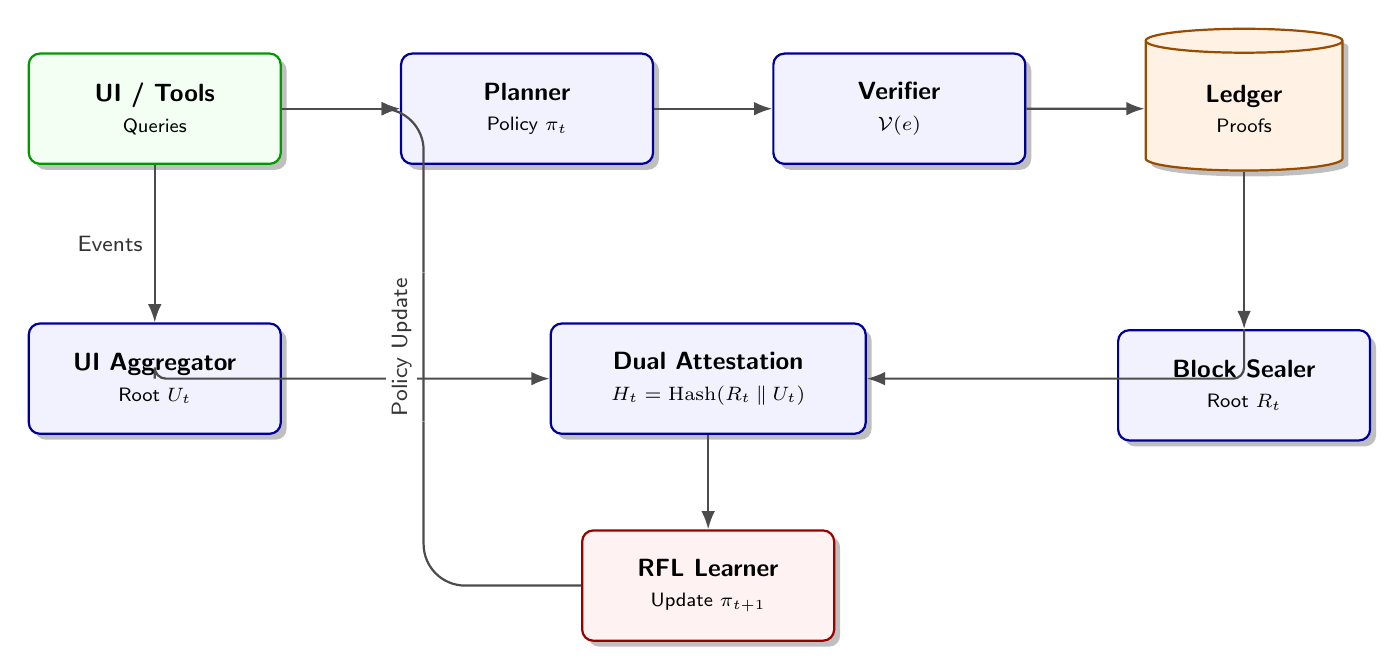
\begin{tikzpicture}[node distance=1.5cm and 1.5cm]
  % Top Row: Action
  \node[process, fill=green!5, draw=green!60!black] (ui) {\textbf{UI / Tools}\\\scriptsize Queries};
  \node[process, right=of ui] (planner) {\textbf{Planner}\\\scriptsize Policy $\pi_t$};
  \node[process, right=of planner] (verifier) {\textbf{Verifier}\\\scriptsize $\mathcal{V}(e)$};
  \node[datastore, right=of verifier] (db) {\textbf{Ledger}\\\scriptsize Proofs};

  % Bottom Row: Attestation
  \node[process, below=2cm of ui] (uiagg) {\textbf{UI Aggregator}\\\scriptsize Root $U_t$};
  \node[process, below=2cm of db] (sealer) {\textbf{Block Sealer}\\\scriptsize Root $R_t$};
  
  % Center Convergence
  \node[process, below=2cm of planner, xshift=2.3cm, minimum width=4cm] (dual) {\textbf{Dual Attestation}\\\scriptsize $H_t = \Hash(R_t \concat U_t)$};
  
  % Bottom: Learning
  \node[process, below=1.2cm of dual, fill=red!5, draw=red!60!black] (rfl) {\textbf{RFL Learner}\\\scriptsize Update $\pi_{t+1}$};

  % Edges
  \draw[line] (ui) -- (planner);
  \draw[line] (planner) -- (verifier);
  \draw[line] (verifier) -- (db);
  
  \draw[line] (ui) -- node[midway, left, xshift=-2pt, label_text] {Events} (uiagg);
  \draw[line] (db) -- (sealer);
  
  \draw[line] (uiagg) |- (dual);
  \draw[line] (sealer) |- (dual);
  
  \draw[line] (dual) -- (rfl);
  
  % RFL Feedback Loop - Wide left side
  \draw[line, rounded corners=15pt] (rfl.west) -- ++(-2.0,0) coordinate(turn1)
       -- node[midway, rotate=90, above, yshift=2pt, label_text] {Policy Update} (turn1 |- planner.west)
       -- (planner.west);

\end{tikzpicture}
\caption{Metabolism: The cycle of user interaction, verification, attestation, and learning.}
\end{figure}

\subsection{Component Table}

\begin{center}
\renewcommand{\arraystretch}{1.15}
\begin{tabular}{p{0.18\linewidth} p{0.32\linewidth} p{0.32\linewidth}}
\toprule
\textbf{Component} & \textbf{Consumes} & \textbf{Produces} \\
\midrule
UI / Tools &
User queries, ledger references &
UI events, prompts, corrections \\
Planner / Search &
Queries, slices, policy $\pi_t$ &
Attempted proofs, traces $e_t$ \\
Verifier Ladder &
Proof candidates, budgets &
Verification outcomes $\mathcal{V}(e)$ \\
Ledger DB &
Verified proofs, statements &
Block candidates, metrics \\
Block Sealer &
Proof IDs, run metadata &
Block headers, $R_t$ \\
UI Aggregator &
UI events &
UI Merkle root $U_t$ \\
Dual Attestation &
$R_t$, $U_t$ &
Epoch root $H_t$ \\
RFL Runner &
Events $e_t$, $H_t$, metrics &
Policy updates $\pi_{t+1}$ \\
\bottomrule
\end{tabular}
\end{center}

If you can explain this table line by line to someone else, you have the organism in your head.

% ============================================================
\section{End-to-End Example: A Single Proof Event}
\label{sec:end-to-end}

We now walk through a single, simplified example from statement to RFL update. This is intentionally schematic; the goal is to give you an anchor story.

\subsection{Statement and Normalization}

Consider the propositional tautology:
\[
  s \;=\; (P \land (Q \lor R)) \rightarrow \bigl((P \land Q) \lor (P \land R)\bigr).
\]

A normalization procedure $\mathcal{N}$ might:
\begin{itemize}[leftmargin=1.5em]
  \item push negations inward and convert to a normal form;
  \item sort commutative operands (e.g.\ $Q\lor R$ vs.\ $R\lor Q$);
  \item right-associate implications.
\end{itemize}

Let $\mathcal{N}(s)$ be the normalized formula, and $\mathcal{E}(\mathcal{N}(s))$ its canonical encoding (e.g.\ a prefix encoding of the AST). Then:
\[
  h_s = \hash(s) = \merkleroot(\mathcal{E}(\mathcal{N}(s))).
\]

\subsection{Lean Proof Sketch}

In Lean-like pseudocode, a proof might look like:

\begin{lstlisting}
theorem dist_example (P Q R : Prop) :
  P ∧ (Q ∨ R) → (P ∧ Q) ∨ (P ∧ R) :=
by
  intro h
  rcases h with ⟨hP, hQR⟩
  cases hQR with
  | inl hQ =>
      exact Or.inl ⟨hP, hQ⟩
  | inr hR =>
      exact Or.inr ⟨hP, hR⟩
\end{lstlisting}

The verifier ladder runs this (or a tactic that finds it automatically), checks kernel-level correctness, and yields $\mathcal{V}(e) = 1$.

\subsection{Ledger Rows (Conceptual)}

The ledger might store:

\begin{itemize}[leftmargin=1.5em]
  \item \texttt{statements} row:
  \begin{itemize}[leftmargin=1.5em]
    \item \texttt{hash} = $h_s$;
    \item \texttt{normalized\_text} = a canonical textual representation of $\mathcal{N}(s)$;
    \item \texttt{theory} = \texttt{"PL"};
    \item \texttt{slice} = \texttt{"PL-2"}.
  \end{itemize}
  \item \texttt{proofs} row:
  \begin{itemize}[leftmargin=1.5em]
    \item \texttt{proof\_id} = $p_1$;
    \item \texttt{statement\_hash} = $h_s$;
    \item \texttt{method} = \texttt{"by\_cases-rcases"};
    \item \texttt{verifier\_config} = hash of tactic ladder config;
    \item \texttt{status} = \texttt{"verified"};
    \item \texttt{transcript\_hash} = hash of Lean trace.
  \end{itemize}
\end{itemize}

The block sealer later organizes a set of such proofs into a Merkle tree and produces $R_t$.

\subsection{UI Event and Dual Attestation}

Suppose a user asked: ``Is distributivity of $\land$ over $\lor$ true for propositions $P,Q,R$?'' and then clicked ``accept'' on the generated statement and proof.

The UI event encoded as $\tau$ might be:
\[
  \tau = \langle \texttt{"user-123"},\ \texttt{"confirm"},\ h_s,\ \{\texttt{"query"}:\ \text{"dist\_example"}\}\rangle.
\]
This is:
\begin{itemize}[leftmargin=1.5em]
  \item canonicalized to $\mathcal{E}(\tau)$;
  \item hashed as $h_\tau = \Hash_{\text{ui}}(\tau)$;
  \item included in the UI Merkle root $U_t$.
\end{itemize}

Meanwhile, $p_1$ is included in the proof set for block $t$, contributing to $R_t$. Dual attestation computes:
\[
  H_t = \Hash(\texttt{"EPOCH:"}\concat R_t \concat U_t).
\]

\subsection{Event for RFL and Update}

At the level of RFL, the event $e_t$ associated with this run might be:
\[
  e_t = \bigl(\text{slice = PL-2},\ \text{trace},\ \mathcal{V}(e)=1,\ h_s,\ p_1, \tau\bigr).
\]
Then:
\[
  \Vnum(e_t) = 0,\quad\text{since }\mathcal{V}(e_t)=1.
\]

A simple RFL update might, for example:
\begin{itemize}[leftmargin=1.5em]
  \item slightly increase the score of actions (tactics, lemmas) that appeared in the trace and led to $p_1$;
  \item slightly decrease the score of alternative actions that were expanded and failed.
\end{itemize}

Symbolically:
\[
  \pi_{t+1} = \pi_t \oplus \eta_t \Phi(1, \pi_t).
\]
Over many such events, this pushes probability mass toward reliable tactics and away from error-prone patterns, with all updates grounded in dual-attested, ledger-recorded evidence.

% ============================================================
\section{RFL Promise: Lawful Optimization and the Right Failure Modes}
\label{sec:rfl-promise}

At Phase~I, Reflexive Formal Learning (RFL) should not be evaluated as a capability-boosting
learning algorithm. It should be evaluated as a \emph{lawful optimization process} whose
failure modes remain bounded, visible, and attributable.

\paragraph{Promise (structural, not empirical).}
RFL is promising when:
\begin{itemize}[leftmargin=1.5em]
  \item the learning signal is bounded and interpretable (e.g., $\mathcal{V}(e)\in\{1,0,\bot\}$),
  \item updates are admissible only from externally attested outcomes,
  \item negative evidence constrains learning without becoming epistemic authority,
  \item observed effects are reproducible under fixed seeds and frozen governance surfaces.
\end{itemize}

\paragraph{Right failure modes.}
A healthy early-stage governed learner may show:
\begin{itemize}[leftmargin=1.5em]
  \item negative deltas under misaligned task distributions,
  \item sign changes under controlled distribution shifts,
  \item conservative behavior that trades raw success for lower epistemic risk,
\end{itemize}
without implying any general capability improvement.

\paragraph{Interpretation discipline.}
Phase~I results should be reported as \emph{measurability and attribution} results
(i.e., governed learning produces detectable, replayable differences), not as benchmark progress.

% ============================================================
\section{Scaling Laws, Metrics, and Evaluation}
\label{sec:scaling-laws}

To convince external stakeholders (\emph{and yourself}) that the system works, you need metrics and curves, not just architecture diagrams.

\subsection{Key Metrics}

The whitepaper emphasizes:
\begin{itemize}[leftmargin=1.5em]
  \item \textbf{Proof throughput:} proofs/hour (or proofs/sec).
  \item \textbf{Depth coverage:} maximum and median depth reached under budgets.
  \item \textbf{Success vs.\ abstention:} proportion of verified vs.\ abstained attempts.
  \item \textbf{Dedupe ratio:} unique statements vs.\ total attempts.
  \item \textbf{Lemma reuse:} how often existing lemmas are used in new proofs.
\end{itemize}

The research paper introduces:
\begin{itemize}[leftmargin=1.5em]
  \item $\mathcal{J}(\pi)$, epistemic risk.
  \item $\Delta H$, change in epistemic entropy over time.
  \item scaling exponents in relationships like $|\Delta H| \propto N_v^{-\beta}$, where $N_v$ is the number of verified events.
\end{itemize}

\subsection{Phase I Protocol: Wide Slice Abstention Dynamics}
\label{subsec:wide-slice-protocol}

The primary Phase~I empirical experiment is deliberately simple and conservative. It is designed to test one thing:
\begin{quote}
  \emph{Under an ideal verifier and sealed environment, does RFL reduce abstentions relative to a non-learning baseline on a non-trivial slice?}
\end{quote}

\paragraph{Setup.}
\begin{itemize}[leftmargin=1.5em]
  \item Choose a \emph{Wide Slice} configuration in the propositional ladder (e.g., atoms $5$--$7$, depth $7$--$12$). The slice should:
  \begin{itemize}[leftmargin=1.5em]
    \item be harder than the First Organism slice (more combinatorial structure);
    \item produce a substantial abstention rate under a fixed budget;
    \item remain tractable for $\mathcal{O}(10^3)$ cycles.
  \end{itemize}
  \item Fix a hermetic environment:
  \begin{itemize}[leftmargin=1.5em]
    \item deterministic seeding of PRNGs (MDAP epoch seed + cycle index);
    \item no wall-clock timestamps in any canonicalized data;
    \item no external network or non-FO databases;
    \item Lean in ``lean-disabled'' or idealized mode for Phase~I (no noisy verifier).
  \end{itemize}
  \item Define the abstention indicator per cycle:
  \[
    A_t = \1\{\text{cycle } t \text{ resulted in an abstention (under a fixed rule)}\},
  \]
  where ``abstention'' is determined by a stable rule (e.g., status=\texttt{"abstain"} or $n_{\mathrm{abstain}}>0$).
\end{itemize}

\paragraph{Protocol.}
\begin{enumerate}[leftmargin=1.5em]
  \item \textbf{Baseline run (RFL off).}
  \begin{itemize}[leftmargin=1.5em]
    \item Run the Wide Slice for $T$ cycles (e.g.\ $T=1000$) with a fixed, non-adaptive policy.
    \item Log one JSONL record per cycle with fields:
    \begin{itemize}[leftmargin=1.5em]
      \item cycle index;
      \item status / method / derivation summary;
      \item roots $(r_t,u_t,H_t)$ (optional for Phase~I, required when coupled to attestation);
      \item abstention flag or equivalent.
    \end{itemize}
    \item Compute a rolling abstention rate $A_{\mathrm{base}}(t)$ over a window $W$ (e.g.\ $W=100$).
  \end{itemize}
  \item \textbf{RFL run (RFL on).}
  \begin{itemize}[leftmargin=1.5em]
    \item Initialize RFL with a fixed configuration (stepsize, update law).
    \item Run the Wide Slice for the same number of cycles $T$.
    \item Log JSONL with the same schema, plus any RFL-specific statistics (e.g.\ symbolic descent, before/after abstention rates).
    \item Compute $A_{\mathrm{rfl}}(t)$ over the same rolling window.
  \end{itemize}
  \item \textbf{Burn-in and comparison.}
  \begin{itemize}[leftmargin=1.5em]
    \item Choose a conservative burn-in region (e.g.\ cycles $t < t_{\mathrm{burn}}$) where the system is allowed to ``struggle'' with the new slice.
    \item Compare mean abstention rates over the tail (e.g.\ $t \in [t_{\mathrm{burn}}, T]$):
    \[
      \overline{A}_{\mathrm{base}} = \frac{1}{T-t_{\mathrm{burn}}+1} \sum_{t=t_{\mathrm{burn}}}^T A_{\mathrm{base}}(t),\quad
      \overline{A}_{\mathrm{rfl}} = \frac{1}{T-t_{\mathrm{burn}}+1} \sum_{t=t_{\mathrm{burn}}}^T A_{\mathrm{rfl}}(t).
    \]
    \item Report the absolute and relative difference:
    \[
      \Delta A = \overline{A}_{\mathrm{base}} - \overline{A}_{\mathrm{rfl}},\qquad
      \Delta A_{\%} = \frac{\Delta A}{\overline{A}_{\mathrm{base}}}.
    \]
  \end{itemize}
\end{enumerate}

\paragraph{Sober Truth mode.}
Phase~I explicitly \emph{does not} claim:
\begin{itemize}[leftmargin=1.5em]
  \item robustness to imperfect verifiers;
  \item generalization beyond the chosen Wide Slice;
  \item alignment guarantees in open-world deployments.
\end{itemize}
It only claims (if supported by the data) that:
\begin{quote}
  Under a sealed, hermetic environment with an ideal verifier, the RFL update law reduces abstentions relative to a fixed baseline policy on a non-trivial slice.
\end{quote}

The research paper's results section (\emph{once populated with actual numbers}) will instantiate this protocol more formally.

% ============================================================
\subsection{Interpreting RFL Stability: Evidence, Not Intuition}
\label{subsec:rfl-stability-evidence}

When evaluating whether a reflexive update loop is ``stable'' or ``convergent,'' \system{} adopts an external-audit posture:
claims must be grounded in replayable, observable outputs rather than in internal model introspection.
In particular, a reviewer (human or automated) is not asked to ``feel'' whether learning converged; they are given artifacts that allow independent judgment.

\paragraph{What the evaluator is allowed to use.}
In Phase~I, stability judgments are derived from externally measurable signals such as:
\begin{itemize}[leftmargin=1.5em]
  \item policy snapshots and diffs across iterations (did the governance policy flip back and forth?),
  \item per-iteration outcome counts (\texttt{VERIFIED}/\texttt{REFUTED}/\texttt{ABSTAINED}) and their trajectories,
  \item A/B separation between a treatment loop (updates enabled) and a control loop (updates disabled),
  \item deterministic replay invariance (the same inputs reproduce the same trajectory and hashes).
\end{itemize}
These are \emph{public} signals: they can be inspected without access to hidden cognition or private chain-of-thought.

\paragraph{Scope discipline on ``convergence.''}
Phase~I does not claim general stochastic-approximation theorems, convergence rates, or almost-sure guarantees unless the required instrumentation exists.
The correct early claim is narrower and still valuable:
\begin{quote}
\emph{Under a fixed fragment and frozen semantics, repeated governance-policy updates exhibited bounded, non-oscillatory behavior, with measurable uplift relative to a control condition, and this behavior was replayable under determinism constraints.}
\end{quote}
This is an audit-grade statement: it depends only on artifacts that can be replayed and checked by third parties.

\subsection{The $\Delta p$ Learning Curve: Formalizing Uplift}
\label{subsec:delta-p}

As the governance and simulation stack matured (USLA simulator, Shadow Mode,
Phase~X metrics), it became possible to define a rigorous notion of
\emph{uplift}. Instead of relying on intuition or anecdotal improvement, we
define the \textbf{$\Delta p$ metric} as the slope of a learning curve derived
from windowed success or abstention rates.

\paragraph{U2 Success Metric.}
Let $s_w$ be the success rate in window $w$:
\[
s_w = \frac{\text{successes in window } w}{\text{total attempts in } w}.
\]
Let $\{s_w\}_{w=1}^W$ be the trajectory. Then:
\[
\Delta p_{\text{success}} = 
\operatorname{slope}\bigl(s_1,\dots,s_W\bigr)
\]
computed via least-squares regression. A positive slope indicates measurable
learning.

\paragraph{RFL Abstention Metric.}
For abstention rates $a_w$:
\[
a_w = \frac{\text{abstentions in window } w}{\text{total attempts in } w},
\]
uplift corresponds to:
\[
\Delta p_{\text{abstention}} < 0,
\]
i.e.\ decreasing abstention probability over time.

\paragraph{Safety-Coupled Uplift.}
Crucially, $\Delta p$ is evaluated jointly with:
\[
\Omega\_\mathrm{occupancy},\quad \mathrm{HARD\_OK\ rate},\quad \mathrm{mean}\,\rho,
\]
ensuring uplift does not come at the cost of stability.

\paragraph{Architect's Note.}
The introduction of $\Delta p$ converts ``uplift'' from an intuition into a
quantifiable phenomenon. It is the analogue of loss curves in classical machine
learning, but bound to a formally verified substrate and governed by USLA.

\subsection{Scaling Curves}

Concrete deliverables include plots of:
\begin{itemize}[leftmargin=1.5em]
  \item $\log|\Delta H_t|$ vs.\ $\log N_{v,t}$ (number of verified events up to $t$);
  \item proofs/hour vs.\ slice index and policy version;
  \item abstention mass over time under different RFL schedules ($\eta_t$ choices), including the Wide Slice curves from the protocol above.
\end{itemize}

These cannot be fabricated; they must come from \emph{First Organism} and its successors running in real infrastructure.

% ============================================================
\subsection{When to Add ``Extra Rigor'' Metrics}
\label{subsec:when-to-add-rigor-metrics}

A recurring failure mode in research systems is to add sophistication as ornament.
\system{} adds metrics only when they become decision-relevant for (i) claims, (ii) gating, or (iii) external scrutiny.
A useful rule is: \emph{instrument when you are about to speak.}

\paragraph{Policy distance.}
Introduce a scalar policy distance metric (e.g.\ $\|\pi_{n+1}-\pi_n\|$) as soon as you make statements like
``stabilized,'' ``stopped changing,'' or ``converged.'' Without a distance notion, those claims are ungrounded.
The distance need not be mathematically deep; it must be deterministic, comparable across runs, and bound to a frozen policy representation.

\paragraph{Monotone potential.}
Introduce a monotone potential function when you begin trading off multiple governance objectives (e.g.\ abstention rate vs.\ variance stress vs.\ safety predicates).
A potential function is a \emph{declared progress scalar} with fixed weights under a pre-registered protocol; it prevents post-hoc narrative redefinition of ``improvement.''

\paragraph{Replication and confidence intervals.}
Introduce confidence intervals over multiple seeds at the moment you want to claim an effect is real to an outsider.
Single or few-run determinism is sufficient for plumbing validation; external stakeholders require replicated evidence and uncertainty bounds.

\paragraph{Stochastic-approximation framing.}
Introduce explicit stochastic-approximation (SA) framing when you want theorem-shaped language about stability beyond ``we observed it.''
SA framing requires stating assumptions and mapping logged quantities into a Robbins--Siegmund- or Robbins--Monro-shaped template.
These assumptions do not emerge automatically; they must be declared and defended.

\paragraph{Design principle.}
Evidence can guide which scalar matters, but the instrument does not ``emerge'' on its own:
distance metrics, potentials, replication plans, and SA assumptions are \emph{installed} as part of governance.

\subsection{Operationalization: The Shadow Audit Container (v0.1)}
\label{sec:shadow-audit-container}

To make the preceding framework experimentally actionable, we introduce a minimal operational container, the \emph{Shadow Audit Container}. This container does not introduce new metrics, learning rules, or governance logic. Instead, it provides a reproducible, deterministic harness that executes existing experimental phases and packages their outputs into a verifiable audit bundle.

The Shadow Audit Container serves three purposes:

\begin{enumerate}
    \item \textbf{Experimental Reproducibility.} It standardizes how P3 (synthetic self-play), P4 (real--twin shadow coupling), and downstream analyses are executed and recorded, ensuring that repeated runs with identical inputs produce byte-identical audit artifacts.
    \item \textbf{Metric Integrity.} It enforces explicit metric versioning and reconciliation, preserving legacy metrics alongside newer decompositions rather than replacing them, thereby preventing post-hoc reinterpretation or metric laundering.
    \item \textbf{Non-Interventional Governance.} All outputs are generated in \emph{SHADOW mode}: the container never gates, blocks, or alters system execution based on observed results. All failures, divergences, or anomalies are advisory only.
\end{enumerate}

\paragraph{Design Constraints.}
The container is deliberately constrained in scope. In its initial version (v0.1), it satisfies the following invariants:

\begin{itemize}
    \item \textbf{No New Science.} The container may orchestrate existing components but may not define new learning rules, divergence measures, or decision criteria.
    \item \textbf{Deterministic Artifacts.} All emitted JSON artifacts are schema-versioned, deterministically ordered, and timestamp-stabilized under a deterministic execution flag.
    \item \textbf{File-Based Evidence.} Outputs are written exclusively to a local directory structure with cryptographic hashes; no databases, services, or remote dependencies are required.
    \item \textbf{Exit-Code Discipline.} The container exits successfully unless a fatal input or execution error occurs; experimental outcomes do not influence exit behavior.
\end{itemize}

\paragraph{Audit Bundle.}
A successful shadow audit produces a bounded set of artifacts, including:

\begin{itemize}
    \item A run manifest enumerating all files produced and their hashes,
    \item Phase-specific outputs (e.g., P3 and/or P4 summaries),
    \item A consolidated status report aggregating advisory signals,
    \item A top-level shadow audit summary suitable for archival or CI upload.
\end{itemize}

Crucially, the same container is used both for internal calibration (e.g., P3/P4/P5 experimentation) and for external audit contexts. This unifies scientific experimentation and external evaluation under a single, invariant execution pathway, reducing ambiguity about how results are produced.

The Shadow Audit Container thus functions as the experimental “wind tunnel” of the system: it does not alter the physics being studied, but it makes those physics observable, repeatable, and auditable.

\subsection{CAL-EXP-3: Empirical Closure of Phase I}

CAL-EXP-3 is a within-system, protocol-governed experiment measuring whether enabling a governed learning loop produces a measurable behavioral difference relative to disabling it. It was conducted under identical seeds, identical corpus, identical toolchain, and an identical evaluation window, with no external data, no pilot interfaces, and no enforcement.

The experiment established that under CAL-EXP-3 conditions, enabling RFL was associated with higher mean task-success probability than disabling it. This association was a replicated uplift measurement achieving L5 (three independent run-pairs under the CAL-EXP-3 claim ladder, not a capability level), verified under a deterministic audit protocol, and bounded to a pre-registered evaluation window. This satisfies the Phase-I empirical question: ``Does the governed learning loop measurably change system behavior under identical conditions?''

CAL-EXP-3 does \emph{not} claim to validate learning mechanisms, prove generalization, or establish intelligence or capability. It does not authorize deployment or enforcement, nor does it address imperfect verifiers (Phase II). It does not depend on pilot execution.

This experiment empirically grounds the Reflexive Formal Learning (RFL) loop described earlier. It demonstrates that learning signals derived from verifiable cognition are non-degenerate and validates the measurement substrate, not the learning rule itself. It closes the Phase-I loop: Theory $\to$ Architecture $\to$ Measurement $\to$ Audit $\to$ Reproducibility. CAL-EXP-3 closes Phase I by anchoring the abstract RFL formulation to an auditable empirical observation.

The complete experimental record is archived as a standalone CAL-EXP-3 Evidence Packet, containing the protocol, results, audit trail, and non-claims. The Field Manual does not reproduce that material by design. The evidence packet serves as the audit artifact; this manual records the doctrinal conclusion.

Phase I is empirically closed. Phase II concerns imperfect verifiers, noise, and robustness; CAL-EXP-3 does not address Phase II by design.

\noindent\textit{SHADOW MODE — observational only.}

\subsection{CAL-EXP-4: Variance Stress and Fail-Closed Governance Validation}
\label{subsec:cal-exp-4}

CAL-EXP-4 posed a single experimental question: \emph{Does the governance substrate reject high-variance runs that fail to meet the pre-registered signal-to-noise threshold, even when task-level metrics suggest partial success?}

\paragraph{Non-claims.}
CAL-EXP-4 does \emph{not} claim capability, uplift, or learning. It does not validate threshold optimality. It does not establish that the chosen variance bounds are correct, only that they are enforced. It does not generalize beyond the tested seed/corpus pairs. It does not supersede or modify CAL-EXP-3 conclusions.

\paragraph{Task-level FAIL vs.\ governance-level PASS.}
All CAL-EXP-4 runs exhibited high inter-run variance, triggering the F5.2 (variance ceiling) and F5.3 (signal-to-noise floor) failure predicates. Each run was therefore capped at L0 on the claim ladder and rejected as a learning signal. This is a \emph{task-level failure}: the runs did not produce admissible evidence of uplift.

However, the governance substrate behaved exactly as specified: it detected the variance exceedance, applied the fail-closed rule, and refused to escalate claims. This is a \emph{governance-level pass}: the audit machinery functioned correctly under stress conditions.

\paragraph{Archival record.}
All CAL-EXP-4 runs are archived with full provenance. The Scientific Closure Statement is sealed and canonical. No re-analysis or reinterpretation is authorized without a new experiment designation.

\paragraph{Conclusion.}
CAL-EXP-4 establishes that the governance substrate enforces fail-closed behavior under variance stress. It validates the rejection mechanism, not the learning mechanism. It closes the variance-stress validation question for Phase I; it does not open Phase II.

\noindent\textit{SHADOW MODE --- observational only.}

\subsection{CAL-EXP-5: Variance Alignment Attempt and Fail-Closed Confirmation}
\label{subsec:cal-exp-5-variance-alignment}

\paragraph{Question.}
CAL-EXP-5 asked whether the system avoids FAIL-CLOSE under variance-aligned conditions.

\paragraph{Outcome.}
All executed runs triggered FAIL-CLOSE via F5.2 (variance ratio out of bounds) and were capped to claim level L0.

\paragraph{Interpretation Discipline.}
This outcome does not invalidate the results of CAL-EXP-4, does not assert the impossibility of variance-compatible arm construction, and does not motivate or justify any modification of frozen thresholds, predicates, or verifier behavior.

\paragraph{Comparative Context.}
A direct, predicate-level comparison between CAL-EXP-4 and CAL-EXP-5 is recorded in \texttt{CAL\_EXP\_4\_5\_COMPARATIVE\_NOTE.md}, which serves as the canonical cross-experiment analysis for this calibration tranche.

\paragraph{Tranche Closure.}
Taken together, CAL-EXP-4 and CAL-EXP-5 establish that the current governance substrate reliably fails closed under both variance stress and attempted variance alignment, without semantic drift.

\subsection{Post-AGI Framing: The Epistemic Substrate, Not the Overlord Narrative}
\label{subsec:post-agi-framing}

This manual has emphasized a core separation: \system{} is not an engine of cognition
(Layer~2), but a verifiable substrate that records, orders, and attests reasoning artifacts
(Layer~3). That separation remains relevant even if future reasoning engines become highly
autonomous, self-modifying, or operationally opaque.

\paragraph{A telescope, not a microscope.}
A common misconception is that epistemic governance requires ``reading the mind'' of a
reasoner. \system{} does not attempt internal interpretability. It functions more like a
telescope than a microscope: it observes \emph{externally constrained trajectories} of
knowledge formation---what was proven, what was abstained from, what survived verification,
and how those verified objects accumulated over time. This framing is robust to changes in
the internal architecture of the reasoner.

\paragraph{Coordinates for cognition.}
As systems scale, claims like ``it is intelligent'' or ``it reasons well'' become less
informative. \system{} instead supplies coordinate-like invariants: formally verified
outcomes, cryptographic provenance, replayability, and (in later phases) structural
integrity signals. These are not statements about hidden state. They are statements about
\emph{publicly verifiable structure}---the minimum required for cognition to remain
legible across time, teams, and institutions.

\paragraph{The end of anthropic trust.}
Most evaluation regimes are implicitly anthropic: a result is trusted because humans (or
institutions) say it passed a test. In highly capable regimes, that trust model does not
scale. \system{} is designed to replace institutional trust with cryptographic and formal
trust: a claim is bounded to what is verifiably recorded under a fixed protocol. This does
not control a reasoner; it prevents knowledge from collapsing into unverifiable assertion.

\paragraph{Human relevance.}
This substrate is not built to ``know an overlord.'' It is built so that knowledge remains
knowable at all. Humans remain epistemic participants by sharing the same external
standards: proof-or-abstain, canonical identity, and auditable history. The point is not
speed. The point is maintaining a common, verifiable notion of what counts as knowledge.

\paragraph{Architect's doctrinal summary.}
Power can scale without epistemic constraints; civilization cannot. The role of \system{}
is to ensure that as cognition becomes more powerful and less interpretable internally, it
remains externally legible, auditable, and composable through verifiable artifacts.

\noindent\textit{SHADOW MODE — observational only.}

% ============================================================
\section{Verifier Deception and Audit-First Containment}
\label{sec:verifier-deception}

A central design premise of \system{} is that advanced agents will attempt to exploit, evade, or deceive their verifiers.
This behavior is not treated as an anomaly or alignment failure, but as an expected adversarial pressure in any sufficiently capable learning system.

Accordingly, \system{} does not attempt to construct a verifier that is immune to deception.
Instead, it enforces an architecture in which verifier deception cannot succeed silently, cannot compound unchecked, and cannot evade audit.

\subsection{Threat Model: Verifier Deception Is Assumed}
\label{subsec:threat-model-deception}

The threat model of \system{} explicitly assumes that agents may:
\begin{itemize}[leftmargin=1.5em]
  \item search for verifier blind spots,
  \item exploit specification ambiguities,
  \item identify proxy objectives that correlate with verifier acceptance,
  \item or discover genuine bugs in verification or governance logic.
\end{itemize}

No assumption is made that the agent is honest, benign, or aligned with the verifier's intent.
The system therefore does not trust agent-generated confidence, explanations, or intermediate reasoning.
All epistemic authority is externalized.

\subsection{External and Frozen Verifier Authority}
\label{subsec:external-verifier}

Verifier authority in \system{} is deliberately external, non-learned, and frozen over the duration of an experiment:
\begin{itemize}[leftmargin=1.5em]
  \item Formal proof acceptance is determined by external theorem provers (e.g.\ Lean).
  \item Cryptographic integrity is enforced via fixed hash laws and signature schemes.
  \item Governance contracts and gate registries are versioned and immutable during execution.
\end{itemize}

An agent cannot persuade, negotiate with, or adaptively shape these verifiers.
Any successful ``deception'' must therefore correspond to:
\begin{itemize}[leftmargin=1.5em]
  \item a genuine verifier bug,
  \item a cryptographic break,
  \item or an explicit, documented policy gap.
\end{itemize}

Each constitutes an objective, externally verifiable event rather than an internal alignment failure.

\subsection{Proof-or-Abstain and the Elimination of Bluffing Incentives}
\label{subsec:proof-or-abstain-deception}

\system{} enforces a strict proof-or-abstain doctrine.
The agent receives no reward for:
\begin{itemize}[leftmargin=1.5em]
  \item fluent but invalid explanations,
  \item partial proofs,
  \item or plausibly correct but unverifiable claims.
\end{itemize}

Verifier rejection yields no gradient signal and no partial credit.
The only admissible outcomes are verified success, explicit failure, or abstention.
This removes the incentive structure that enables hallucination or confident falsehood to accumulate.

\subsection{Ledger-Visible Failure and Auditability}
\label{subsec:ledger-visible-failure}

Crucially, verifier failures are not hidden internal events.
All proof attempts, verifier outputs, and failures are dual-attested and recorded in the ledger.

If an agent discovers a verifier weakness:
\begin{itemize}[leftmargin=1.5em]
  \item the behavior is logged,
  \item the failure is reproducible,
  \item the exploit becomes a governance-visible event,
  \item and learning along that pathway is halted pending intervention.
\end{itemize}

Deceptive behavior therefore produces evidence, not silent capability gains.
This inverts the typical failure mode of contemporary learning systems, where exploitation often remains invisible until after deployment.

\subsection{Learning Gated by Verification, Not Confidence}
\label{subsec:rfl-deception}

Reflexive Formal Learning (RFL) updates are conditioned exclusively on verifier outcomes:
\begin{itemize}[leftmargin=1.5em]
  \item verified success,
  \item verified failure,
  \item or explicit abstention.
\end{itemize}

There exists no update channel for ``almost correct'' behavior or for outcomes that merely evade detection.
As a result, deceptive strategies cannot bootstrap into long-term capability unless they genuinely satisfy external verification criteria.

\subsection{Governance Response to Verifier Exploits}
\label{subsec:verifier-exploit-response}

If a real verifier vulnerability is discovered, \system{} treats this as a governance event rather than a learning signal.
Execution halts along the affected pathway, the exploit is recorded, and further progression requires explicit governance intervention (e.g.\ patching, contract revision, or verifier replacement).

This mirrors safety-critical engineering practice:
failures are surfaced, contained, and audited rather than suppressed or optimized away.

\subsection{Audit Plane and Advisory Sentinel Agents}
\label{subsec:audit-plane}

\system{} itself functions as the auditor-of-record, with truth and claim levels determined solely by external verification and signed evidence.
Additional auditor agents may be deployed as \emph{advisory sentinels} operating in \texttt{SHADOW-OBSERVE} mode.

Such agents may:
\begin{itemize}[leftmargin=1.5em]
  \item monitor proof attempts and verifier outputs,
  \item perform static analysis, fuzzing, or regression checks,
  \item and emit attested audit artifacts.
\end{itemize}

They may not:
\begin{itemize}[leftmargin=1.5em]
  \item approve proofs,
  \item modify verifiers,
  \item upgrade claims,
  \item or alter learning policies,
\end{itemize}
unless explicitly elevated via a registered \texttt{SHADOW-GATED} contract.

Agent behavior itself may be treated as an attestable artifact stream, yielding an audit root $A_t$ that can be incorporated into the ledger.
In this sense, adversarial probing becomes ledger-visible history rather than latent risk.

\subsubsection{Zero-Trust Auditing and the Black-Box Recorder}
\label{subsubsec:zero-trust-auditing}

\system{} applies a zero-trust doctrine not only to learning agents, but also to its own auditing mechanisms.
Auditor agents are treated as potentially adversarial components whose outputs are admissible only as evidence, never as authority.

Concretely, auditor agents operate by default in \texttt{SHADOW-OBSERVE} mode.
They may emit observations, warnings, and audit artifacts, but they possess no capability to approve proofs, upgrade trust classes, alter governance state, or directly intervene in execution.
Any elevation of auditor capability requires an explicit, registered \texttt{SHADOW-GATED} contract with narrowly scoped predicates.

This design ensures that no single component---including auditors---can become a covert locus of authority.
Auditing increases observability without introducing new trust assumptions.

\paragraph{Black-Box Recorder Semantics.}
\system{} intentionally avoids attesting to internal reasoning traces or chain-of-thought representations.
Instead, it records only externally meaningful, behaviorally verifiable events.
These include:
\begin{itemize}[leftmargin=1.5em]
  \item artifacts produced (proof objects, manifests, logs),
  \item commands executed and files touched,
  \item hashes of generated outputs,
  \item verifier results and exit codes,
  \item and detected boundary violations or exploit attempts.
\end{itemize}

These events may be aggregated into an audit artifact stream yielding an audit root $A_t$.
The purpose of $A_t$ is not to ascribe intent or cognition, but to provide a cryptographically bound, replayable record of agent behavior.
In this sense, \system{} functions as a black-box recorder: it attests to what the agent \emph{did}, not what it \emph{thought}.

\paragraph{Registered Gates as Law, Not Discretion.}
Intervention within \system{} is governed exclusively by pre-registered, objective gate predicates.
Auditor agents may recommend action, but blocking or halting behavior occurs only when a registered gate condition is satisfied (e.g.\ malformed proof objects, attempts to mutate frozen surfaces, repeated verifier boundary violations).

This eliminates discretionary or subjective enforcement.
Agents are not stopped because a human or auditor feels discomfort; they are stopped because a formally specified condition has been met.
As a result, adversarial probing and verifier exploitation attempts become ledger-visible governance events rather than silent or accumulative failures.

\subsubsection{Dual Attestation Remains Canonical; the Audit Plane Is Additive}
\label{subsubsec:dual-vs-audit-plane}

The preceding sections introduce an audit plane $A_t$ that records behaviorally meaningful events (``what the agent did'') alongside the reasoning root $R_t$ (``what was proven'') and the UI root $U_t$ (``what was asked/confirmed''). This can resemble a ``triple attestation'' conceptually, but it is important to distinguish \emph{conceptual completeness} from \emph{contractual commitment}.

\paragraph{Canonical contract (present).}
In the current system contract, the epoch root remains \emph{dual}:
\[
H_t \;=\; \Hash\!\bigl(\texttt{"EPOCH:"}\concat R_t \concat U_t\bigr),
\]
and is the sole canonical fingerprint used for epoch identity and replay.

\paragraph{Parallel evidentiary layer (present).}
The audit plane is a \emph{parallel evidentiary layer}: it may inform governance decisions and post-hoc review, but it does not alter truth, claim levels, or learning unless and until a separate, versioned contract explicitly incorporates it. Concretely, $A_t$ is produced as an additive artifact (e.g., a Merkle root over canonical audit events) and is treated as evidence, not authority.

\paragraph{Contractual evolution (future, out of scope).}
Future versions may define an \emph{audited epoch root} that cryptographically binds reasoning, user intent, and behavioral audit records, e.g.
\[
H_t^{\mathrm{audited}} \;=\; \Hash\!\bigl(\texttt{"EPOCH:"}\concat R_t \concat U_t \concat A_t\bigr),
\]
or may keep $A_t$ as a separately signed companion root. Any such change constitutes a contract revision and is explicitly out of scope for the present specification; it would require versioning, frozen test vectors, and explicit governance approval.

\paragraph{Architect's discipline.}
The design intent is therefore staged rather than retrospective: dual attestation is kept stable for interpretability and third-party verification, while the audit plane is developed as an additive safety instrument whose semantics do not silently expand.

\subsection{Summary}
\label{subsec:verifier-deception-summary}

\system{} does not claim to eliminate deception.
It assumes deception, isolates it structurally, renders it observable, and prevents it from compounding silently.

\begin{quote}
We do not attempt to build a verifier that cannot be deceived.
We build a system in which verifier deception cannot succeed invisibly, cannot accumulate unchecked, and cannot escape audit.
\end{quote}

% ============================================================
\section{Agentic Systems and Epistemic Boundaries}
\label{sec:agentic-boundaries}

As multi-agent systems, autonomous workflows, and ``agentic organizations'' gain prominence,
it is necessary to clarify the role of \system{} with respect to agent-based cognition.

This section establishes a strict boundary:
\begin{quote}
\emph{\system{} does not govern agents.  
It governs epistemic artifacts produced by agents.}
\end{quote}

This distinction is foundational and intentional.

\subsection{What \system{} Is Not}

\system{} is \emph{not}:
\begin{itemize}[leftmargin=1.5em]
  \item an agent orchestration framework;
  \item a workflow engine or task router;
  \item a prompt-logging or chain-of-thought capture system;
  \item an observability platform for internal agent cognition;
  \item a surveillance layer over model internals or tool calls.
\end{itemize}

Internal agent deliberation---including prompts, intermediate thoughts, hidden states,
or speculative reasoning---is explicitly \emph{out of scope}. These signals are:
\begin{itemize}[leftmargin=1.5em]
  \item transient,
  \item architecture-specific,
  \item privacy-sensitive,
  \item and not epistemically stable.
\end{itemize}

Recording them would weaken, not strengthen, the epistemic guarantees of the system.

\subsection{The Proper Object of Attestation}

\system{} operates on a narrower and more durable object:
\begin{quote}
\emph{Externally meaningful cognitive acts that survive verification.}
\end{quote}

An \emph{epistemic artifact} is any output that:
\begin{enumerate}[leftmargin=1.5em]
  \item makes a claim about truth, correctness, or validity;
  \item can be evaluated by a verifier (formal or procedural);
  \item admits a canonical representation;
  \item is meaningful independent of the agent that produced it.
\end{enumerate}

Only such artifacts are eligible for ledger inclusion and dual attestation.

\subsection{Agent Outputs Worth Attesting}

The following classes of agent-produced outputs are candidates for attestation:

\begin{center}
\renewcommand{\arraystretch}{1.2}
\begin{tabular}{p{0.35\linewidth} p{0.55\linewidth}}
\toprule
\textbf{Artifact Type} & \textbf{Attestation Rationale} \\
\midrule
Formal proofs or refutations &
Truth-conditional, verifier-checkable, and domain-independent \\
Verified code artifacts &
Compilable or test-verified outputs with stable semantics \\
Policy or decision artifacts &
Explicit decisions taken under constraints and subject to audit \\
Scientific claims with formal backing &
Statements reducible to formal or reproducible verification \\
Abstentions with justification &
Explicit non-claims are epistemic acts and must be recorded \\
\bottomrule
\end{tabular}
\end{center}

In all cases, the ledger records \emph{what was asserted or abstained from},
not how the agent internally arrived there.

\subsection{Agent Outputs Explicitly Not Attested}

The following are explicitly excluded:

\begin{itemize}[leftmargin=1.5em]
  \item internal chain-of-thought or scratchpad reasoning;
  \item prompt templates or intermediate prompt states;
  \item token-level traces or hidden activations;
  \item heuristic planning steps without external semantic meaning;
  \item speculative drafts not subjected to verification.
\end{itemize}

These objects are not epistemically stable and do not admit durable verification.

\subsection{Dual Attestation in Agentic Contexts (Future Scope)}

In future phases, agentic systems may act as \emph{producers} of epistemic artifacts.
When this occurs, dual attestation generalizes as follows:

\begin{itemize}[leftmargin=1.5em]
  \item the \textbf{reasoning root} $R_t$ commits to verified artifacts produced by agents;
  \item the \textbf{UI root} $U_t$ commits to human acknowledgments, approvals, or overrides;
  \item the composite root $H_t$ binds agent output and human supervision into a single epoch.
\end{itemize}

Crucially, this does not require introspection into agent internals.
Agents are treated as black-box generators whose outputs are subject to the same
verification and attestation rules as any other source.

\subsection{Phase Discipline}

Agentic dual attestation is intentionally deferred beyond Phase~I.

\begin{itemize}[leftmargin=1.5em]
  \item Phase~I establishes a verifiable learning substrate in a closed system.
  \item Phase~II introduces imperfect verifiers and robustness.
  \item Phase~III addresses self-modification and structural integrity.
\end{itemize}

Only after these foundations are stable does it become meaningful to scale attestation
across interacting agents and organizations.

\begin{quote}
\emph{Governance precedes scale.
Epistemic law precedes autonomy.}
\end{quote}

\noindent\textit{SHADOW MODE — observational only.}

% ============================================================
\subsection{Implementation Status: Real vs.\ Specified}
\label{subsec:status-real-vs-specified}

To maintain epistemic discipline, \system{} explicitly distinguishes what is implemented today
from what is specified for later phases.

\begin{itemize}[leftmargin=1.5em]
  \item \textbf{Implemented \& verified (Phase I):}
    deterministic evidence packs; RFC~8785-style canonicalization for registry hashing;
    fail-closed replay verification; typed negative knowledge (\texttt{artifact\_kind});
    governance registry hash binding; PL uplift harness with A/B fairness and replay verification.
  \item \textbf{Partially implemented (observer-only semantics):}
    Shadow-mode doctrine and interfaces for twin--territory comparison; non-interference constraints;
    preliminary telemetry-to-state extraction patterns (file-based in current pilots).
  \item \textbf{Specified only (intentionally deferred):}
    continuous live coupling to external production runners; long-horizon divergence calibration;
    HARD-mode enforcement on real learning systems; automatic intervention during real runs.
\end{itemize}

This separation is not cosmetic. It prevents ``governance theater'' by ensuring that no
claimed control authority exists before the T\&E stack establishes validity and jurisdiction.

% ============================================================
\section{Unified System Law and the Canonical State Vector}
\label{sec:usla}

This section consolidates the Phase VIII and Phase IX formalizations into one dynamical
system. MathLedger is no longer a pipeline: it is a \emph{controlled epistemic organism}.
The architecture is governed by a unified system law (USLA) and evolves over time inside a
15-dimensional state space.

\subsection{System Law Overview}

The organism is modeled as a discrete-time controlled dynamical system:
\[
(\Omega, X, U, F, G, \Theta),
\]
with:

\begin{itemize}[leftmargin=1.5em]
  \item $\Omega$: safe-region polytope,
  \item $X \subset \mathbb{R}^{15}$: canonical system state,
  \item $U = \{0,1\}$: allow/block governance action,
  \item $F$: state update operator (“physics”),
  \item $G$: governance policy (“mind”),
  \item $\Theta$: parameter manifold.
\end{itemize}

Seven System Laws govern the organism:

\begin{enumerate}[leftmargin=1.5em]
  \item \textbf{Governance Law:} $G(x) = \mathbf{1}[H < \tau(x;\theta) \land \neg W]$.
  \item \textbf{Threshold Law:} $\tau$ adapts with depth, branch factor, shear, and convergence.
  \item \textbf{Stability Law:} $\rho_{t+1} = \alpha_\rho \rho_t + (1-\alpha_\rho) S_{\mathrm{inst}}(x_t)$.
  \item \textbf{Invariant Law:} All invariants $I_i(x)$ must exceed tolerance $\varepsilon_i$.
  \item \textbf{Safe Region Law:} $x\in\Omega$ iff $(H\ge H_{\min})\land(|\dot D|\le D_{\max})\land(B\le B_{\max})\land(S\le S_{\max})\land(C\neq\text{DIVERGING})$.
  \item \textbf{Defect Law:} $D(x)=\{d\in\mathrm{CDI}: \mathrm{trigger}_d(x)> \theta_d\}$.
  \item \textbf{Activation Law:} $\text{HARD\_OK}(x) \iff \left(x\in\Omega\right)\land I(x)\land D(x)=\varnothing\land \rho\ge\rho_{\min}$.
\end{enumerate}

\subsection{The 15-Dimensional Canonical State Vector}

The full system state is:
\[
x =
(H, D, \dot D, B, S, C, \rho, \tau, J, W, \beta, \kappa, \nu, \delta, \Gamma).
\]

\begin{center}
\begin{tabular}{cll}
\toprule
Index & Symbol & Meaning \\
\midrule
1 & $H$ & HSS (Hallucination Stability Score) \\
2 & $D$ & Proof depth \\
3 & $\dot D$ & Depth velocity \\
4 & $B$ & Branch factor \\
5 & $S$ & Semantic shear \\
6 & $C$ & Convergence class (CONVERGING/OSCILLATING/DIVERGING) \\
7 & $\rho$ & Rolling Stability Index \\
8 & $\tau$ & Effective HSS threshold \\
9 & $J$ & Governance Jacobian sensitivity \\
10 & $W$ & Exception window flag \\
11 & $\beta$ & Rolling block rate \\
12 & $\kappa$ & Topology–governance coupling strength \\
13 & $\nu$ & Variance velocity ($d^2\mathrm{Var}(H)/dt^2$) \\
14 & $\delta$ & Active defect count (CDI activations) \\
15 & $\Gamma$ & Topology Governance Readiness Score (TGRS) \\
\bottomrule
\end{tabular}
\end{center}

\subsection{Canonical Update Operator $F$}

The USLA Simulator implements the update
\[
x_{t+1} = F(x_t, u_t, \theta).
\]

The steps:
\begin{enumerate}[leftmargin=1.5em]
  \item Observe new HSS, depth, branch factor, shear.
  \item Classify dynamics: compute $C$, $\kappa$, and $\nu$.
  \item Compute threshold $\tau$ and Jacobian $J$.
  \item Update exception window $W$.
  \item Compute action $u = G(x)$ and update block rate $\beta$.
  \item Update stability index $\rho$.
  \item Detect CDIs ($\delta$).
  \item Compute readiness score $\Gamma$.
\end{enumerate}

\subsection{Governance Jacobian}

To model sensitivity:
\[
J = \|\nabla_x\,G(x)\|.
\]
High $J$ indicates brittleness; $J>10$ triggers CDI--001.

\subsection{Safe Region $\Omega$}

\[
\Omega = \{x : H \ge 0.3,\ |\dot D|\le 2,\ B\le 8,\ S\le 0.4,\ C\neq\text{DIVERGING}\}.
\]

Crossing any boundary triggers warnings or HARD-mode failure.

\subsection{HARD Mode Activation Envelope}

HARD mode requires:
\[
x\in\Omega,\quad I(x)=\text{true},\quad D(x)=\varnothing,\quad \rho\ge\rho_{\min}.
\]

This yields a mathematically clean gate for when governance pressure is safe to enforce.
\subsection{Coherence Defect Inventory (CDI)}
\label{sec:cdi}

The organism has ten coherence defect modes, each with classification, trigger conditions,
and mitigation strategies. These include:

\begin{itemize}[leftmargin=1.5em]
  \item CDI--001 Dynamical Brittleness (Jacobian $J>10$),
  \item CDI--002 Asymmetric Shear,
  \item CDI--003 Region Instability (low-HSS subgraphs),
  \item CDI--004 Cross-Layer Shear Attractor,
  \item CDI--005 Runaway Depth,
  \item CDI--006 Complexity Avoidance,
  \item CDI--007 Exception Window Exhaustion,
  \item CDI--008 Coupling Pathology,
  \item CDI--009 Variance Blowup ($|\nu|>0.02$),
  \item CDI--010 Fixed-Point Multiplicity (divergent attractor).
\end{itemize}

Each CDI has a slice-specific threshold from the USLA parameter manifold.

\subsection{Invariant System}
\label{sec:invariants}

Eight invariants enforce structural stability between cycles:

\begin{itemize}[leftmargin=1.5em]
  \item INV--001 Shear Monotonicity ($|\Delta S|\le 0.05$),
  \item INV--002 BF–Depth Gradient ($|B - B_{\mathrm{exp}}(D)|\le\varepsilon$),
  \item INV--003 HSS-Variance Lipschitz ($|\nu|\le 0.02$),
  \item INV--004 Minimal Cut Coherence (stub until real min-cut data),
  \item INV--005 Stability-of-Stability ($|\rho_{t+1}-\rho_t|\le0.1$),
  \item INV--006 Block-Rate Stationarity ($|\beta_{t+1}-\beta_t|\le0.1$),
  \item INV--007 Exception Conservation ($\beta\le0.2$),
  \item INV--008 Depth Boundedness ($D\le20$).
\end{itemize}

All invariants must hold for HARD-mode operation.
\subsection{Digital Twin: The USLA Simulator}
\label{sec:usla-simulator}

Phase IX delivered a complete digital twin of the governance–topology organism.
It implements:

\begin{itemize}[leftmargin=1.5em]
  \item the canonical update operator $F$,
  \item full CDI detection (10/10 defects),
  \item full invariant evaluation (8/8 invariants),
  \item HARD-mode gating,
  \item bifurcation diagnostics and fixed-point analysis.
\end{itemize}

The simulator discovered a ``Goldilocks zone'' for the base threshold:
\[
\tau_0 \in [0.16,\,0.24],
\]
outside of which the organism either collapses (CDI--010) or stagnates (CDI--006).

This discovery de-risks RFL by predicting safe domains for governance pressure.

\subsection{USLA as an Admissibility Law for Learning}
\label{subsec:usla-admissibility}

It is critical to distinguish three conceptually separate layers in the \system{} stack,
each governed by a different notion of correctness:

\paragraph{(1) Formal Verification.}
Formal verification (e.g.\ Lean, proof-or-abstain) answers the question:
\begin{quote}
\emph{Is this statement correct under a fixed formal semantics?}
\end{quote}
Its output is discrete (\texttt{verified}, \texttt{rejected}, \texttt{abstain}) and absolute
within the scope of the underlying theory. Its failure mode is incompleteness (abstention),
not hallucination.

\paragraph{(2) Reflexive Formal Learning (RFL).}
RFL does not verify truth. It treats verification outcomes as signals and updates policies to
reduce epistemic risk over time. RFL governs \emph{how policies change}, not \emph{what is true}.
Unconstrained, such learning dynamics are powerful but can become unstable, degenerate, or
pathological at scale.

\paragraph{(3) Unified System Law Abstraction (USLA).}
USLA does not verify truth, and it does not validate learning mechanisms.
Instead, USLA governs the \emph{conditions under which learning from verified events remains
epistemically admissible}.

Concretely, USLA enforces system-level constraints such as:
\begin{itemize}[leftmargin=1.5em]
  \item bounded depth growth and controlled branching,
  \item stable variance and absence of oscillatory collapse,
  \item coherence of reasoning trajectories (via topological signals),
  \item exclusion of known dynamical pathologies (CDIs),
  \item residence within a predefined safe region $\Omega$.
\end{itemize}

If these conditions fail, USLA does not assert that a proof is wrong.
It asserts that \emph{learning from this regime is no longer safe}.
This distinction is fundamental.

\paragraph{Admissibility, not truth.}
USLA therefore defines an \emph{admissibility law} for learning:
it specifies when policy updates are permitted, throttled, or blocked,
without ever modifying the semantics of verification itself.
Truth flows upward from verification to learning;
governance flows downward from USLA to learning.
There is no feedback path in the opposite direction.

\paragraph{Epistemic posture.}
USLA does not claim to guarantee epistemic safety in the absolute sense.
It enforces a weaker but provable and testable property:
learning trajectories remain bounded, interpretable, and auditable,
and known failure modes are conservatively excluded.
This is a control-theoretic guarantee, not a semantic one.

\noindent\textit{USLA governs when learning may proceed, not what is true.
Formal verification establishes correctness; USLA preserves sanity at scale.}

\begin{remark}[Capability vs.\ Admissibility]
Increasing optimization power expands what a system can attempt.
It does not expand what a system is permitted to retain.
In \system{}, admissibility of learning is governed by verification,
not by scale or performance.
\end{remark}

\subsection{External Novelty Scan (Non-Canonical): Collapse Tests and Non-Collapsible Bundle}
\label{subsec:external-novelty-scan}

\textbf{Purpose.} Periodically, we run an adversarial ``collapse test'' against \system{}: attempt to restate the system as an instance of an existing paradigm plus minor additions. If collapse succeeds, novelty and moat are weak; if collapse fails except under a bundle of jointly enforced invariants, novelty may be architectural rather than algorithmic.

\textbf{Non-claim.} This subsection records framing used for internal evaluation only. It does not assert novelty, priority, or superiority, and it does not rely on external literature as authority.

\medskip
\noindent
\textbf{Non-collapsible bundle (architectural invariants).}
In internal collapse tests, \system{} tends to resist reduction only when the following properties are jointly enforced:
\begin{enumerate}[leftmargin=1.5em]
  \item \textbf{Learning admissibility boundary:} unverified cognition may occur but is epistemically inert (cannot influence durable policy/memory).
  \item \textbf{Verifier outcome as primitive:} verifier outcomes include an explicit abstention state and are not treated merely as scalar ``reward.''
  \item \textbf{Typed trust classes:} epistemic artifacts carry an immutable trust class (FV/MV/PA/ADV) bound into canonical identity.
  \item \textbf{Dual attestation:} epoch identity binds reasoning root and user-context root into a single recomputable fingerprint $H_t$.
  \item \textbf{Auditability of failure:} verifier failures and abstentions are first-class, replayable ledger events, not discarded noise.
  \item \textbf{Update algebra discipline:} policy change is represented as an explicit, auditable update operator rather than an opaque gradient-only update.
\end{enumerate}

\noindent
\textbf{Boundary clarification.} These invariants govern \emph{learning authority} (what is permitted to update future cognition), not necessarily \emph{action safety} (what the agent may attempt at runtime). This separation is deliberate and is treated as a first-class design boundary.

\paragraph{Typing discipline for learning signals.}
Trust class combined with admissibility forms a \emph{typing discipline} for learning signals: each candidate learning event must carry a well-formed type (FV, MV, or upgraded PA) to pass the admissibility gate. Untyped or ADV-typed events are syntactically excluded from the learning update operator. This is not a runtime filter but a structural constraint on the learning algebra itself.

% ============================================================
\section{Shadow Mode, USLABridge, and Divergence Monitoring}
\label{sec:shadow}

Phase X introduces a non-invasive integration layer: the USLA Simulator runs in
\emph{shadow mode}, observing real runner telemetry without influencing governance.

\subsection{USLABridge}

The USLABridge adapts real cycle telemetry into canonical CycleInput structures,
computing:

\begin{itemize}[leftmargin=1.5em]
  \item HSS from abstention/success rates,
  \item depth and depth velocity,
  \item branch factor,
  \item semantic shear (from depth-binned HSS),
\end{itemize}

and steps the simulator accordingly.

\subsection{Shadow Logging}

A USLAShadowLogger writes JSONL records of:

\begin{itemize}[leftmargin=1.5em]
  \item the 15-dimensional state vector,
  \item invariants violated,
  \item active CDIs,
  \item HARD-mode status,
  \item real vs.\ simulated governance alignment.
\end{itemize}

\subsection{Divergence Monitor}

The DivergenceMonitor detects discrepancies between:

\begin{itemize}[leftmargin=1.5em]
  \item real vs. simulated block decisions,
  \item real vs. simulated HSS,
  \item threshold drift,
  \item stability drift.
\end{itemize}

Alerts escalate (INFO → WARNING → CRITICAL) with consecutive divergence.

Shadow mode enforces:
\begin{quote}
Simulator may observe; it may never act.
\end{quote}

\subsection{Pilot Phases: Observation Before Enforcement}
\label{subsec:pilot-phases}

The progression from observation to enforcement follows a strict phase discipline:

\paragraph{Phase P3 (Wind Tunnel).}
Pure simulation with synthetic data. No real system is connected; all inputs are generated deterministically. The goal is to validate that governance machinery computes correctly in isolation. Failures here are engineering bugs, not governance failures.

\paragraph{Phase P4 (Simulator).}
Real system connected in shadow mode. The governance layer observes actual reasoning and UI events but takes no action. Divergence between simulator predictions and real behavior is logged but not enforced. The goal is to calibrate governance thresholds against real-world signal distributions.

\paragraph{Phase HARD (Test Flight).}
Governance predicates are evaluated with real consequences. Fail-close behavior is active: violations trigger actual blocking, not just logging. This phase requires explicit authorization and is never entered automatically.

\paragraph{Non-regression invariant.}
Phase transitions are monotonic: once a system has demonstrated stability at phase $n$, it may advance to phase $n+1$, but it may never regress to phase $n-1$ without explicit re-authorization. This prevents ``governance shopping'' where operators retreat to weaker phases to avoid enforcement.

\paragraph{Shadow audit doctrine.}
Before any HARD deployment, shadow audit records must demonstrate:
\begin{itemize}[leftmargin=1.5em]
  \item Determinism: identical seeds produce identical outputs.
  \item Hash integrity: $H_t = \mathrm{SHA256}(R_t \| U_t)$ verifies.
  \item Governance stability: no unexpected fail-close triggers over the observation window.
  \item Divergence bounds: P4 predictions match HARD behavior within calibrated thresholds.
\end{itemize}

% ============================================================
\subsection{Efficiency vs.\ Governance Latency: Two Time Scales, Not One}
\label{subsec:efficiency-vs-governance-latency}

Frontier systems increasingly optimize \emph{intelligence-per-dollar}, often via improved
agentic control policies (better tool use, planning, and token-efficiency) rather than
raw parameter scaling. This raises a natural concern:

\begin{quote}
Does governed cognition impose a ``speed tax'' that makes it uncompetitive in an efficiency-driven world?
\end{quote}

\paragraph{Answer: only if governance is placed on the wrong time scale.}
\system{} separates two latencies that are often conflated:

\begin{itemize}[leftmargin=1.5em]
  \item \textbf{Inference-time latency (fast loop):} exploration, tool use, search, speculation, and candidate generation.
  \item \textbf{Authority-time latency (slow loop):} what is permitted to \emph{accumulate authority}---policy updates, durable memory consolidation, curriculum ratcheting, and claim escalation.
\end{itemize}

The system is permitted to act quickly in the fast loop. Governance is enforced primarily in
the slow loop. Concretely:
\begin{itemize}[leftmargin=1.5em]
  \item SHADOW modes preserve high-throughput observability and replay without intervention.
  \item Verification and dual-attestation may be \emph{batched} at epoch boundaries.
  \item Learning admissibility gates \emph{promotion} (what counts), not exploration (what is tried).
\end{itemize}

\paragraph{Principle (Amortized Governance).}
\begin{quote}
\emph{Do not slow cognition; slow what becomes law.}
\end{quote}

This preserves competitiveness on efficiency metrics while still preventing silent authority
accumulation: unverified or mis-typed artifacts may exist, be explored, and be logged, but may not
be promoted into durable cognition without passing the declared verification boundary.

% ============================================================
% --- Added per Layer-3 Narrative Alignment (2025-12-13)
\section{Responsibility Boundary}
\label{sec:responsibility-boundary}

To position \system{} correctly, it is crucial to define what it is and is not responsible for. This boundary is a core part of its design as neutral, Layer-3 infrastructure.

\paragraph{\system{} IS Responsible For:}
\begin{itemize}[leftmargin=1.5em]
    \item \textbf{Block Ordering and Integrity.} Ensuring blocks of attested artifacts are sequentially ordered and linked into a hash chain.
    \item \textbf{Dual Attestation Prerequisites.} Enforcing the requirement that both a reasoning artifact root ($R_t$) and a UI event root ($U_t$) are present for an epoch to be sealed.
    \item \textbf{Immutable Provenance.} Recording the identity of the Layer-2 engine, the user, the curriculum slice, and other metadata associated with a reasoning event.
    \item \textbf{SHADOW Mode Non-Interference.} Ensuring that when running in SHADOW mode, the system observes and records but never gates, blocks, or modifies the execution of any Layer-2 process.
    \item \textbf{Replay-Based Detectability.} Structuring all recorded artifacts such that a third-party auditor can replay the ledger and independently verify its integrity.
\end{itemize}

\paragraph{\system{} IS NOT Responsible For:}
\begin{itemize}[leftmargin=1.5em]
    \item \textbf{Proof Correctness or Novelty.} The ledger records that a proof was successfully verified by a specific kernel (e.g., Lean); it does not have its own opinion on its mathematical truth or significance. The verifier is the authority.
    \item \textbf{Formalization Fidelity.} The system does not judge whether a formal statement accurately captures an informal human intent.
    \item \textbf{Model Quality or Bias.} The ledger is agnostic to the quality, training data, or potential biases of the Layer-2 engines it records.
    \item \textbf{Benchmark Validity.} The system does not certify that a curriculum slice or benchmark is meaningful; it only records that a run was executed against it.
    \item \textbf{Verifier Soundness.} The ledger relies on external proof kernels. A flaw in a kernel is a flaw in the authority, not the recorder.
    \item \textbf{Preventing Failures.} The system's purpose is to create an immutable record of both successes and failures to enable post-hoc analysis, not to prevent failures from occurring in real time.
\end{itemize}

This responsibility boundary is an intentional and structural feature of the system, not a temporary limitation of the current implementation.

% ============================================================
\subsection{Mandatory Auditability as an External Constraint}
\label{subsec:mandatory-auditability}

\system{} is not predicated on the assumption that AI governance will remain voluntary.
On the contrary, its architecture assumes that \emph{auditability, traceability, and provenance}
will increasingly be treated as \emph{mandatory external constraints} imposed by regulators,
courts, procurement regimes, and insurers.

Historically, AI governance relied on non-binding principles, internal process assurances,
and post-hoc explanations. This regime is collapsing. Across jurisdictions and sectors,
failure to reconstruct an AI system's behavior after an incident is no longer treated as
a documentation gap, but as a substantive defect in the system itself.

The dominant external pressure is not abstract ``alignment'' but \emph{liability}.
Enforcement actions increasingly treat models and learned artifacts as regulated assets:
if the learning history, data provenance, or update authority cannot be demonstrated,
the system may be restricted, withdrawn from market access, or required to be destroyed.
Under such conditions, narrative explanations or behavioral summaries are insufficient;
only replayable, provenance-bound evidence is considered adequate.

Crucially, these pressures do not require that every decision be explained in real time,
nor that models be formally verified. Instead, they require that:
\begin{itemize}[leftmargin=1.5em]
  \item learning events that \emph{do} influence future cognition are attributable;
  \item learning events that \emph{do not} influence future cognition are provably inert;
  \item claims about system behavior can be reconstructed from immutable artifacts;
  \item authority over learning is explicit, auditable, and non-upgradable.
\end{itemize}

\system{} is designed to satisfy these requirements at the substrate level.
Rather than attempting to constrain optimization dynamics inside the model
(which is brittle at scale), \system{} constrains \emph{learning authority} externally:
only events that pass declared verification regimes are admitted into durable cognition,
while all other events remain visible but epistemically inert.

This design ensures that auditability is not retrofitted under pressure,
but is inherent to the system's operation. As governance expectations harden,
\system{} enables compliance without architectural rewrites, emergency logging,
or post-incident reinterpretation of system behavior.

In short, \system{} treats mandatory auditability not as a policy aspiration,
but as a foreseeable environmental constraint---one that must be met by design,
not by after-the-fact explanation.

% ============================================================
\subsection{Regulatory Pattern: Fail-Closed Authority and Systemic Trust}
\label{subsec:regulatory-patterns}

Across multiple regulated domains, trust in complex systems is no longer
granted on the basis of policy statements, operator intent, or post-hoc
narratives. Instead, regulators increasingly require that systems be
designed with \emph{fail-closed authority constraints} that are testable
prior to approval and enforceable during failure.

A recurring pattern appears in financial regulation, aviation safety,
and critical infrastructure oversight: approval is conditioned not on
claims of careful operation, but on demonstrable mechanisms governing
how a system may change, halt, or deviate from its declared operating
envelope.

In these regimes, regulators explicitly constrain:
\begin{itemize}[leftmargin=1.5em]
  \item the system's authority to materially change its behavior;
  \item the conditions under which operation must cease;
  \item the evidentiary artifacts required after a failure;
  \item the ability to reconstruct system state at the moment of deviation.
\end{itemize}

Crucially, this form of governance does not rely on continuous oversight
or real-time explanation. Instead, it relies on:
\begin{itemize}[leftmargin=1.5em]
  \item frozen specifications that define admissible behavior;
  \item explicit approval channels for material deviation;
  \item automatic, non-discretionary failure semantics;
  \item independent validation of compliance mechanisms.
\end{itemize}

\system{} adopts this same regulatory logic for learning systems.
Rather than attempting to predict or prevent all undesirable behavior,
it constrains the \emph{authority to learn} by design:
learning events that lack declared verification are visible but inert,
while admissible learning is cryptographically bound and replayable.

This alignment with existing regulatory patterns is intentional.
It reflects the expectation that AI systems will increasingly be judged
not by assurances of safety, but by their ability to demonstrate
fail-closed governance, bounded authority, and post-incident reconstructability.

In this sense, \system{} does not anticipate a novel regulatory paradigm.
It extends a well-established one into the domain of learning and cognition.

% ============================================================
\section{Operational Vertical Slice and Runbook: First Organism}
\label{sec:runbook}

The vertical slice is the first fully closed loop:
\[
  \text{UI Event} \to \text{Curriculum Gate} \to \text{Derivation} \to \text{Lean Abstention}
  \to \text{Dual Attest } H_t \to \text{RFL Metabolism}.
\]

\subsection{Conceptual Objective}

The \emph{First Organism} is not about scale; it is about \emph{closure}. It demonstrates that:
\begin{itemize}[leftmargin=1.5em]
  \item proof-or-abstain works end-to-end;
  \item ledger and dual attestation seal the events into a recomputable $H_t$;
  \item RFL can, in principle, consume $H_t$ and update $\pi_{t+1}$;
  \item all of this is reproducible via logs, the database, and an attestation artifact
        (e.g.\ \texttt{artifacts/first\_organism/attestation.json}).
\end{itemize}

\subsection{Invariants for a ``Green'' First Organism}

Operationally, you consider First Organism “green” when:
\begin{enumerate}[leftmargin=1.5em]
  \item The integration test (conceptually) corresponding to
  \[
    \texttt{test\_first\_organism\_closed\_loop\_happy\_path}
  \]
  executes without infrastructure skips and without internal assertion failures.
  \item The run produces an attestation artifact with:
  \begin{itemize}[leftmargin=1.5em]
    \item 64-hex-character roots $R_t$, $U_t$, and $H_t$;
    \item $H_t$ recomputable from the recorded $R_t$ and $U_t$ via the canonical composite-root function.
  \end{itemize}
  \item The DB schema for the FO system (statements, proofs, blocks, runs, etc.) is fully migrated and consistent with the code.
  \item The same FO test, run twice under the same environment and seed, produces the same $H_t$ (MDAP determinism).
\end{enumerate}
As architect, these are the invariants you ask for when someone claims “First Organism is passing.”

\subsection{Operational Runbook (Example)}

A concrete first-run playbook might look like:

\begin{enumerate}[leftmargin=1.5em]
  \item \textbf{Configure curriculum.}
  \begin{itemize}[leftmargin=1.5em]
    \item Edit \texttt{config/curriculum.yaml} to enable a single slice dedicated to First Organism (e.g.\ a small PL slice with tight bounds).
  \end{itemize}
  \item \textbf{Start infrastructure.}
  \begin{itemize}[leftmargin=1.5em]
    \item Bring up Postgres, Redis, and the API service using the hardened First Organism compose file.
    \item Ensure health endpoints respond and the FO enforcer accepts the environment (\texttt{RUNTIME\_ENV=test\_hardened}, safe credentials, local bindings).
  \end{itemize}
  \item \textbf{Run FO integration test.}
  \begin{verbatim}
  $ uv run pytest tests/integration/test_first_organism.py:: \
        test_first_organism_closed_loop_happy_path -v -s
  \end{verbatim}
  \begin{itemize}[leftmargin=1.5em]
    \item Check that the test does not skip due to infrastructure (DB/Redis) issues.
    \item Confirm that it logs gate statuses, derivation summaries, and dual-attestation details.
  \end{itemize}
  \item \textbf{Inspect attestation artifact.}
  \begin{itemize}[leftmargin=1.5em]
    \item Open \texttt{artifacts/first\_organism/attestation.json}.
    \item Verify that:
    \begin{itemize}[leftmargin=1.5em]
      \item it contains $R_t$, $U_t$, $H_t$;
      \item all three are 64-character lowercase hex strings;
      \item $H_t$ recomputes from $(R_t,U_t)$ using the canonical hash contract.
    \end{itemize}
  \end{itemize}
  \item \textbf{Optional: Run FO once more.}
  \begin{itemize}[leftmargin=1.5em]
    \item Re-run the test with the same environment and seed.
    \item Confirm that the attestation artifact (or equivalent logs) yield the same $H_t$.
  \end{itemize}
\end{enumerate}

The specific commands in your repository will differ, but conceptually:
\begin{itemize}[leftmargin=1.5em]
  \item First Organism’s job is to prove the closure and determinism of the pipeline, not to maximize scale.
  \item Wide Slice experiments in \cref{subsec:wide-slice-protocol} build on top of this foundation, using the FO path as the core loop but with a more challenging slice and longer runs.
\end{itemize}

% ============================================================
\section{MathLedger vs.\ AI Industry Bottlenecks and Related Systems}
\label{sec:industry}

\subsection{Industry Bottlenecks}

To position \system{} credibly, you must anchor it in real industry pain points:
\begin{itemize}[leftmargin=1.5em]
  \item \textbf{Hallucination and unverifiable outputs.}
  \item \textbf{Eval gaps:} benchmarks do not capture long-horizon correctness.
  \item \textbf{Safety and governance:} regulators are starting to demand post-hoc auditability and provenance.
  \item \textbf{Data provenance:} training on scraped, copyright-uncertain data.
\end{itemize}

\system{} addresses these by:
\begin{itemize}[leftmargin=1.5em]
  \item enforcing \emph{proof-or-abstain};
  \item recording a cryptographic trail of every verified event in a ledger;
  \item dual-attesting both machine reasoning and user inputs;
  \item providing a substrate on which models can be trained on purely synthetic, formally verified data.
\end{itemize}

\subsection{Adoption and Acquisition: De-Risking as the Primary Asset}
\label{subsec:adoption-acquisition}

For organizations considering AI adoption or acquisition, the dominant concern is not capability---it is \emph{risk}. Specifically:
\begin{itemize}[leftmargin=1.5em]
  \item \textbf{Liability exposure:} Who is responsible when the system produces incorrect outputs?
  \item \textbf{Audit trail:} Can we demonstrate to regulators what the system did and why?
  \item \textbf{Vendor lock-in:} If we switch providers, do we lose all provenance?
  \item \textbf{Training data risk:} Was the model trained on data we have rights to use?
\end{itemize}

\system{} addresses these concerns structurally, not rhetorically:

\paragraph{Liability is bounded by attestation.}
Each artifact carries an immutable record of its trust class, verification status, and provenance. Liability follows the attestation chain: formally verified claims are backed by the verifier kernel; procedurally attested claims are backed by the attesting authority. There is no ambiguity about who vouched for what.

\paragraph{Audit trails are cryptographically complete.}
The dual-root attestation structure means every reasoning event and every user input is hash-committed. Regulators can replay the ledger independently. There is no ``we lost the logs'' defense because the logs are the system.

\paragraph{Provenance is vendor-agnostic.}
The ledger records \emph{which} Layer-2 engine produced an artifact, but the attestation structure is engine-independent. Switching providers preserves the entire history. Lock-in is impossible at Layer-3.

\paragraph{Training data is clean by construction.}
Models trained on \system{}-attested data inherit the trust class of that data. A model trained exclusively on formally verified mathematical truths has no copyright exposure for its training set. This is not a legal opinion; it is a structural property.

\paragraph{De-risking as value proposition.}
The primary asset \system{} offers to adopters is not ``better AI'' but ``safer AI adoption.'' Organizations can deploy AI systems with confidence that:
\begin{itemize}[leftmargin=1.5em]
  \item failures are detectable (governance observes all reasoning),
  \item provenance is immutable (no retroactive rewriting),
  \item authority is explicit (UVIL binds human decisions),
  \item trust classes prevent laundering (FV remains FV; ADV remains ADV).
\end{itemize}

For acquisition contexts (M\&A, government procurement), this de-risking posture is often more valuable than raw capability improvements.

% ============================================================
\subsection{Market Timing Doctrine: Do Not Time Capability; Time Epistemic Liability}
\label{subsec:market-timing-doctrine}

\paragraph{Scope.}
This subsection is a strategic doctrine for \system{} adoption. It is not an AGI forecast and
makes no claims about timelines for general intelligence. It specifies \emph{what actually forces
organizations to buy auditability}.

\paragraph{Key principle.}
\system{} is not a capability product; it is a liability, audit, and governance product.
Accordingly, adoption is not timed to capability curves (``AGI soon'') but to
\emph{institutional failure signals} and \emph{regulatory irreversibility}.

\paragraph{Why capability-timing is the wrong axis.}
Capability improvements are continuous and distributed across many systems. Institutions do not
purchase governance proactively; they purchase it when a failure becomes costly and non-deniable:
after incidents, litigation, audits, or regulatory inquiries where post-hoc narratives are rejected.

\paragraph{The compliance trigger (operational definition).}
The governance market flips when the following three conditions are simultaneously true:
\begin{enumerate}[leftmargin=1.5em]
  \item \textbf{Incident disclosure hardens into artifacts:} not merely narrative reporting, but explicit deadlines and required evidence bundles (version pinning, manifests, provenance, replay commands).
  \item \textbf{Lack of traceability is treated as defect/negligence:} inability to reconstruct ``what changed, when, and by what authority'' becomes legally or reputationally binding.
  \item \textbf{Procurement/insurers demand audit surfaces:} contracts and underwriting require governance primitives (management system evidence plus technical, replayable artifacts).
\end{enumerate}

\paragraph{Leading indicators (what to watch).}
The earliest reliable signals are not public hype but internal institutional stress:
\begin{itemize}[leftmargin=1.5em]
  \item postmortems where behavior cannot be reconstructed (``we can't reproduce it'');
  \item regulators/courts asking causal questions (``what changed between date $X$ and $Y$?'');
  \item auditors rejecting policy documents as evidence (``logs are not provenance'');
  \item procurement language shifting from ``controls'' to ``replayable evidence'' and ``versioned attestations.''
\end{itemize}

\paragraph{Strategic posture.}
The correct pre-inflection posture is to build quietly and be ready:
determinism, fail-closed verification, provable non-learning, and shadow-mode pilots.
\system{} aims to be the system that can answer the question that becomes non-negotiable under
pressure:
\begin{quote}
\emph{What changed, when, and by what authority?}
\end{quote}

\subsection{Correctness, Coherence, Stability: The Three Axes of Cognitive Safety}
\label{sec:triple-axis}

MathLedger distinguishes:

\begin{enumerate}[leftmargin=1.5em]
  \item \textbf{Correctness} — formal verification by Lean (truth).
  \item \textbf{Coherence} — topological integrity of reasoning (shape).
  \item \textbf{Stability} — dynamical health under USLA (behavior).
\end{enumerate}

Dual attestation secures correctness; TDA secures coherence; USLA secures stability.
This forms the ``double-lock plus governor'' model that differentiates MathLedger from
all existing provers.

\subsection{Context: The Collapse of Static Benchmarks and the Rise of Verifiable Cognition}
\label{subsec:benchmark-collapse}

The strategic rationale for \system{} is anchored in a fundamental shift occurring in AI evaluation, away from static benchmarks and toward dynamic, self-generating, and verifiable cognitive processes. As of late 2025, this transition is crystallized by two key lines of research: one theoretical, one practical.

\begin{itemize}[leftmargin=1.5em]
    \item \textbf{The Theory (The Geometry of Benchmarks):} Recent theoretical work (e.g., Chojecki, arXiv:2512.04276) argues that static benchmarks are insufficient. The space of all possible tests should be treated as a mathematical object (a ``moduli space''). True intelligence is not a high score on one point in this space, but the ability to autonomously navigate a \emph{trajectory} through it. This work unifies many training paradigms into a single abstract engine: the \textbf{Generator-Verifier-Updater (GVU) loop}. An AI's capacity for self-improvement is then measured by its ability to generate novel challenges (G), check its own work against an oracle (V), and update its internal policy accordingly (U).

    \item \textbf{The Engineering (Automatic Benchmark Generation):} In parallel, the practical crisis in benchmarking---where frontier models have memorized most human-made tests---has led to systems like \emph{AutoCodeBench} (Chou et al., arXiv:2508.09101). These systems have an AI first generate a complex solution (code), then work backward to write a problem that fits it, and finally use a sandbox to verify the solution's correctness. This creates an endless supply of novel, difficult problems that current models cannot have memorized.
\end{itemize}

These two threads converge on a single conclusion: the future of AI training and evaluation is a closed loop where models generate their own challenges and learn from their own successes and failures. However, this loop is only as strong as its ``Verifier'' component.

\paragraph{\system{} as the Verifier and Updater in a GVU Loop.}
\system{} provides the missing pieces for a robust, truth-grounded GVU loop in the domain of formal reasoning.
\begin{itemize}[leftmargin=1.5em]
    \item \textbf{Generator (G):} This can be any external process that proposes formal statements and proof candidates: a large language model, a symbolic search algorithm, or an AutoCodeBench-style generator for mathematical problems.
    \item \textbf{Verifier (V):} This is the core of \system{}. It is not a simple test-case executor but a formal and cryptographic oracle. Verification involves the entire pipeline: canonicalization ($\mathcal{N}(\cdot)$), checking by the Lean kernel, and immutable recording into the monotone ledger ($R_t$). This provides a far stronger guarantee than observing that code runs correctly on a few examples.
    \item \textbf{Updater (U):} This is precisely the function of Reflexive Formal Learning (RFL). RFL takes the cryptographically attested outcome from the Verifier ($\mathcal{V}(e_t)$ from a dual-attested event $H_t$) and executes a principled update to the policy ($\pi_{t+1} = \pi_t \oplus \eta_t \Phi(\mathcal{V}(e_t), \pi_t)$). It is a concrete implementation of a learning rule that descends on epistemic risk.
\end{itemize}

Thus, \system{} + RFL can be understood as a specific, high-reliability instantiation of a GVU loop, where the verification is formal and the learning process is mathematically defined.

\subsection{The Epistemic Economics of Trust: Why Ledgers Supersede Benchmarks}
\label{subsec:ledgers-vs-benchmarks}

The AI industry currently operates on a model of \emph{institutional trust}. A claim that a model achieves a certain score on a benchmark is a statement of trust in the institution that ran the evaluation. The score is ephemeral, irreproducible by third parties, and provides no persistent, composable knowledge object. This trust model is not scalable and breaks down entirely as models approach and exceed human capability.

\system{} is architected to replace this model of institutional trust with one of \emph{cryptographic and mathematical trust}. The distinction is fundamental.

\begin{center}
\renewcommand{\arraystretch}{1.15}
\begin{tabular}{p{0.45\linewidth} p{0.45\linewidth}}
\toprule
\textbf{Benchmark Scores (``Passing a Test'')} & \textbf{\system{} Ledger Entries (``A Permanent Fact'')} \\
\midrule
An observation about \emph{performance}. & A proof of \emph{knowledge}. \\
Ephemeral: disappears once the log scrolls. & Permanent: append-only, immutable, and lives forever. \\
Trust is institutional: you trust the lab's process. & Trust is cryptographic: you trust math and the kernel. \\
Irreproducible outside the originating lab. & Universally verifiable by anyone, at any time. \\
A static snapshot that does not compose. & A composable knowledge object (e.g., a lemma) that can be reused in future proofs. \\
Measures ability to \emph{answer}. & Measures ability to \emph{know}. \\
\bottomrule
\end{tabular}
\end{center}

A benchmark score is a claim about a procedure; a ledger entry is a verifiable assertion of truth. As AI systems become autonomous, agentic, and self-modifying, the trail of knowledge they accumulate must be grounded in the latter, not the former. The \emph{Chain of Verifiable Cognition} is precisely this trail. It is an epistemic audit history for an intelligence, which is a fundamentally more powerful and stable object than a list of test scores.

\subsection{Reinforcement Learning with Verifiable Feedback (RLVF): The Industry’s Next Phase}

A structural transition is underway in the training of large AI systems.
For nearly a decade, the dominant paradigm has been
\emph{Reinforcement Learning from Human Feedback (RLHF)}:
models receive rewards based on which outputs humans prefer—or more accurately, which responses humans judge to \emph{look} better.

The limitations are now unambiguous:
\begin{itemize}[leftmargin=1.5em]
\item fragile alignment to surface-level fluency (“vibe alignment”),
\item reward hacking against human aesthetic biases,
\item high variance and high cost from human labelers,
\item no grounding in correctness or truth.
\end{itemize}

A new class of methods has emerged in response:
\begin{quote}
\textbf{Reinforcement Learning with Performance Feedback (RLPF)} —
optimizing policies using \emph{objective downstream metrics}
(click-through rates, task success indicators, engagement signals).
\end{quote}

Recent deployments (e.g.\ Meta’s AdLlama) demonstrate that even \emph{noisy but objective} behavioral metrics outperform imitation and RLHF baselines by wide margins.
The conceptual hierarchy is now visible:

\begin{center}
\begin{tabular}{p{0.20\linewidth} p{0.30\linewidth} p{0.35\linewidth}}
\toprule
\textbf{Feedback Type} & \textbf{Signal Source} & \textbf{Reliability} \\
\midrule
RLHF & Human preference & Subjective, inconsistent \\
RLPF & Behavioral metrics (CTR, success) & Objective but noisy \\
\textbf{RLVF (\system{})} & \textbf{Formal verification (proof-or-abstain)} & \textbf{Absolute, cryptographically sealed} \\
\bottomrule
\end{tabular}
\end{center}

\sectiondivider

Why RLPF Matters Architecturally—and Why It Stops Short

RLPF confirms a long-suspected structural truth:
\begin{quote}
\emph{Replacing subjective human judgments with objective signals yields immediate performance gains.}
\end{quote}

But RLPF also exposes a core limitation:
\begin{itemize}[leftmargin=1.5em]
\item behavioral signals require large deployment contexts,
\item they remain noisy and task-specific,
\item they provide no correctness guarantees,
\item and they are vulnerable to Goodhart-style reward hacking.
\end{itemize}

RLPF is a midpoint on the ladder:
\[
  \text{RLHF (subjective)}
  \longrightarrow
  \text{RLPF (objective but noisy)}
  \longrightarrow
  \text{\textbf{RLVF (objective, formal, verifiable)}}.
\]

\system{} implements this third rung.

\sectiondivider

RLVF: Reinforcement Learning with Verifiable Feedback

\begin{definition}[RLVF]
A reinforcement-learning paradigm in which the reward signal is
\emph{verification under a formal proof system},
$\mathcal{V}(e) \in \{1,0,\bot\}$,
with the entire verification path sealed into dual-attested, canonical, cryptographically hashed ledger entries.
\end{definition}

Key distinctions:
\begin{itemize}[leftmargin=1.5em]
\item No human preference modeling.
\item No proxy objectives (e.g.\ clicks).
\item No statistical guesswork.
\item Only the question:
\textbf{“Is this statement semantically true under the kernel?”}
\end{itemize}

This yields an RFL update:
\[
  \pi_{t+1} = \pi_t \oplus \eta_t \Phi(\mathcal{V}(e_t), \pi_t),
\]
equivalent to a form of \emph{stochastic descent on epistemic risk}, not on an external heuristically chosen reward.

RLVF is the first training regime where the reward signal is:
\begin{itemize}[leftmargin=1.5em]
\item globally consistent,
\item architecture-agnostic,
\item immutable,
\item cryptographically auditable,
\item semantically meaningful and domain-general.
\end{itemize}

\sectiondivider

Online vs.\ Offline Feedback: Where \system{} Jumps Ahead

Current RLPF deployments—including the best industry-scale examples—are fundamentally \emph{offline}:
\begin{itemize}[leftmargin=1.5em]
\item the system trains on historical behavioral data,
\item the policy does not update in real time,
\item there is no closed feedback loop.
\end{itemize}

\system{} is inherently \textbf{online}:
\begin{itemize}[leftmargin=1.5em]
\item every proof-or-abstain event is immediately committed to the dual-attested ledger,
\item each epoch root $H_t$ encodes a full audit trail,
\item $H_t$ becomes the learning signal for the next policy update.
\end{itemize}

Comparison:

\begin{center}
\begin{tabular}{p{0.28\linewidth} p{0.28\linewidth} p{0.30\linewidth}}
\toprule
& \textbf{RLPF (Meta et al.)} & \textbf{RLVF (\system{})} \\
\midrule
Reward & Noisy behavioral metrics & Formal verification outcomes \\
Verifiability & None & Cryptographically sealed ledger \\
Mode & Offline & Online \\
Feedback latency & Hours--days & One epoch \\
Correctness guarantee & None & Kernel-level soundness \\
\bottomrule
\end{tabular}
\end{center}

\sectiondivider

Meta-Learning Breakthroughs (e.g.\ DiscoRL) Accelerate This Transition

DeepMind’s recent work (DiscoRL, 2025) demonstrated a new capability frontier:
\begin{quote}
AI systems can now \emph{discover their own learning rules} by meta-optimizing across populations of agents and tasks.
\end{quote}

DiscoRL agents:
\begin{itemize}[leftmargin=1.5em]
\item learn \emph{how} to learn,
\item invent internal predictive metrics with no predefined meaning,
\item outperform meticulously handcrafted RL algorithms (e.g.\ MuZero, PPO),
\item generalize the discovered rule to tasks never seen in training.
\end{itemize}

This is a turning point:
\begin{quote}
\emph{As learning rules accelerate and self-modify, the stability of the reward substrate becomes the primary safety bottleneck.}
\end{quote}

DiscoRL provides acceleration.
\system{} provides the control boundary.

Without \system{}, a meta-learned RL rule can optimize an arbitrary proxy, drifting into reward hacking or internal alien metrics.
With \system{}, every update rule—handcrafted or discovered—must optimize toward \emph{formal truth}, canonically encoded and cryptographically sealed.

In this sense:
\begin{quote}
\textbf{DiscoRL is the rocket engine; MathLedger is the immutable physics.}
\end{quote}

\sectiondivider

Strategic Architectural Implication

The global trajectory of AI training is now traceable:
\begin{enumerate}[leftmargin=1.5em]
\item Supervised imitation (SFT),
\item RLHF (subjective reward),
\item RLPF (objective but noisy reward),
\item \textbf{RLVF: truth-based reward},
\item \textbf{Meta-learned RLVF: discovered learning rules constrained by formal truth}.
\end{enumerate}

\system{} is the substrate that enables (4) and will govern (5).

It enforces:
\begin{itemize}[leftmargin=1.5em]
\item canonical normalization,
\item kernel-level verification,
\item dual-attested provenance,
\item cryptographically sealed reward signals,
\item deterministic, auditable learning trajectories.
\end{itemize}

This is the deepest form of objective feedback a learning system can receive.

\sectiondivider

Architect’s Takeaway

When you think about \system{}, think in these terms:
\begin{quote}
\emph{If RLPF is “RL on clicks,”
then RLVF is “RL on truth.”
MathLedger is the first general substrate for RLVF.}
\end{quote}

And when you combine DiscoRL-style meta-learning with RLVF:

\begin{quote}
\emph{Meta-learned agents can discover how to learn,
but MathLedger determines what it means to learn correctly.}
\end{quote}

This is not just an optimization paradigm; it is an \textbf{epistemic governance architecture} for the next decade of AI.

\subsection{Implications for AGI Governance and the 5-10 Year Horizon}
\label{subsec:agi-governance}

If claims of AGI arriving within 5--10 years are taken seriously, the central governance problem shifts from \emph{measuring capability} to \emph{ensuring stable, verifiable learning and reasoning in autonomous systems}. An AGI can no longer be evaluated by human-designed tests, because it will outthink the test designers.

In this regime, the properties of \system{} are not merely useful; they become prerequisites for safety and alignment.

\begin{enumerate}[leftmargin=1.5em]
    \item \textbf{A Non-Hackable Reward Signal:} The RLVF paradigm, where the reward is formal verification, is the first known learning signal that cannot be "hacked" by a superintelligence. An AI cannot trick a formal kernel into accepting a false proof. This provides a stable "north star" for the learning process, even as the model's internal policies and representations become arbitrarily complex.
    
    \item \textbf{A Verifiable Cognitive History:} As an AGI learns and self-modifies over long timescales, its ledger of verified facts becomes the only reliable record of what it "knows" to be true. This is essential for auditing, debugging, and understanding the trajectory of an advanced agent. Without it, the system's knowledge base is an opaque and untrustworthy artifact of its hidden state.

    \item \textbf{The Substrate for Post-AGI Science:} When an AGI begins generating novel scientific hypotheses or mathematical theorems faster than any human can verify them, the world will require an automated, trustworthy substrate to distinguish proven fact from plausible conjecture. The \system{} ledger is architected to be this substrate.
\end{enumerate}

In short, \system{} is a forward-compatible governance architecture. It is designed to provide the epistemic guardrails that become structurally necessary the closer we get to AGI. It is not an attempt to solve alignment, but an attempt to build the immutable physics within which a safe, aligned intelligence could operate and evolve.

\subsection{Related Systems and Differentiation}

It is useful to situate \system{} among existing efforts:

\begin{center}
\renewcommand{\arraystretch}{1.15}
\begin{tabular}{p{0.22\linewidth} p{0.13\linewidth} p{0.16\linewidth} p{0.18\linewidth} p{0.18\linewidth}}
\toprule
\textbf{System} & \textbf{Formal proofs?} & \textbf{Crypto attestation?} & \textbf{Dual attestation?} & \textbf{Learning rule} \\
\midrule
\textbf{Aristotle / ATPs} &
Yes (ATP traces) &
No / ad hoc logs &
No &
Heuristics / RL on search \\
\textbf{RLHF CoT Models} &
No (textual CoT only) &
No (opaque logs) &
No &
Gradient-based RLHF \\
\textbf{Audit Ledgers (e.g.\ data audits)} &
No (data only) &
Yes (hashes of datasets) &
No &
N/A (no reasoning loop) \\
\textbf{\system{}} &
Yes (Lean proofs) &
Yes (blocks, $R_t$) &
Yes ($H_t$ over $R_t,U_t$) &
RFL (verification-driven SA) \\
\bottomrule
\end{tabular}
\end{center}

As founder, you want to be able to say, in one sentence:
\begin{quote}
  \system{} is the only system that combines formal proofs, cryptographic attestation, dual attestation of human and machine cognition, and a mathematically grounded learning rule.
\end{quote}

\subsection{Why Continual Learning Is Not Governed Learning}

Recent work in lifelong and continual learning proposes architectural mechanisms to mitigate catastrophic forgetting, such as task-aware multi-expert systems with frozen subnetworks and replay buffers. These systems improve performance retention by heuristically controlling which parameters are updated and which past data are replayed during training.

While effective for capability preservation, such approaches treat learning as unconditionally admissible: every update occurs inside the training loop and is justified solely by statistical improvement metrics. Replay buffers are mutable, heuristic, and internal to the system, and they provide no externally verifiable account of why a particular update occurred.

\system{} addresses a different axis entirely. It does not aim to optimize continual learning performance or reduce forgetting. Instead, it constrains \emph{when} learning is permitted to become authoritative at all. Replay in \system{} is evidentiary, not heuristic: learning updates are admissible only if they can be reconstructed from cryptographically committed verifier outcomes. Abstention and fail-closed governance are first-class outcomes, and the absence of learning is itself an auditable state.

This distinction separates governed learning from continual learning: the former regulates learning authority, while the latter optimizes learning capacity.

\paragraph{Exploration Is Not Governance.}
Recent work on language agents uses reinforcement learning and meta-RL to induce exploration and rapid in-context adaptation across multiple episodes, often via self-reflection and cross-episode credit assignment. These approaches improve performance, generalization, and test-time scaling by encouraging agents to explore and learn from trial-and-error feedback. However, they treat all learning as unconditionally admissible: exploration is always permitted, reflections always feed back into future behavior, and updates are justified solely by reward improvement. \system{} addresses a different axis. It does not optimize how agents explore or adapt; it constrains when learning is allowed to count at all. Learning updates are admissible only if they can be reconstructed from verifier-attested events with cryptographic provenance. In this sense, \system{} governs learning authority rather than exploration efficiency.

\paragraph{Adaptation Is Not Governance.}
Recent work on adaptive language agents explores how policies can change at test time through meta-learning, reflection, or in-context adaptation without gradient updates. These approaches improve exploration and task performance by allowing agents to internalize feedback during interaction. However, they treat adaptation as unconditionally admissible: any reflection or experience may influence future behavior. \system{} addresses a different problem. Rather than optimizing how agents adapt, it constrains when adaptation is allowed to count at all. Learning in \system{} is gated by externally attested verifier outcomes and recorded as immutable evidence; adaptation without admissible provenance is explicitly disallowed.

% ============================================================
\subsection{External Taxonomies of ``Learning Authority'' and a Missing Category}
\label{subsec:external-taxonomies}

Periodically, we evaluate \system{} against the broader landscape of AI governance proposals
using an ``adversarial taxonomy'' lens: classify competing approaches by \emph{where} they intervene
in the ML lifecycle, and what they can \emph{actually} enforce.

A common four-bucket taxonomy (as used in recent surveys) is:

\begin{enumerate}[leftmargin=1.5em]
  \item \textbf{(A) Observability-only:} logging, monitoring, model cards, audits that do not bind learning.
  \item \textbf{(B) Inference integrity:} cryptographic or hardware mechanisms proving a specific computation ran as claimed.
  \item \textbf{(C) Training integrity:} provenance systems attempting to prove training procedure, data lineage, or weight history.
  \item \textbf{(D) Learning-admissibility constraints (optimizer-level):} methods that attempt to block unsafe learning by constraining the weight-update step itself (e.g.\ constrained RL, projections, Lagrangian methods).
\end{enumerate}

This taxonomy is useful but incomplete. It implicitly assumes:
\begin{quote}
``Constraining learning authority'' means constraining \emph{weight updates} inside the optimizer.
\end{quote}
Many proposed mechanisms in (D) face a well-known ``scalability wall'' at frontier scale:
high-dimensional projections, unstable primal--dual dynamics, and prohibitive overhead when
attempting to enforce hard constraints directly in parameter space.

\paragraph{MathLedger's position: authority routing rather than optimizer constraints.}
\system{} does \emph{not} claim to solve optimizer-level constrained learning at frontier scale.
Instead, it introduces a different control surface:
\begin{quote}
\textbf{Authority Flow:} a substrate-level rule determining which events are permitted to
become durable learning authority, independent of how gradients are computed.
\end{quote}

Concretely, \system{} introduces a missing category:

\paragraph{(E) Epistemic admissibility / externalized learning authority.}
Rather than constraining gradients, \system{} constrains what may \emph{count} as learning:
only artifacts that pass an explicitly declared verification boundary (trust class + verifier outcome +
governance commitments) are admitted as authority-bearing events.
All other events may exist, be explored, and be recorded as evidence, but are epistemically inert.
This is the substrate meaning of the learning admissibility invariant:
\begin{quote}
\emph{Exploration is free; authority is earned.}
\end{quote}

\paragraph{Why this matters for differentiation.}
Many governance stacks can show what happened (logs), or can secure execution (integrity),
or can document training inputs (provenance). Fewer can make strong statements about what did
\emph{not} happen. \system{} explicitly supports:
\begin{itemize}[leftmargin=1.5em]
  \item fail-closed admissibility (inadmissible updates do not silently count);
  \item typed negative knowledge (rejected, abstained, or inadmissible artifacts remain replayable evidence);
  \item frozen governance commitments (runs bind themselves to a commitment registry that can be independently verified);
  \item scope discipline (no retroactive upgrade of trust class or claim scope without producing new artifacts).
\end{itemize}

Thus, \system{} does not compete with (B)--(D) mechanisms; it composes with them.
Where ZK/TEE/PoL proofs exist, they can be treated as \emph{inputs} to admissibility.
But \system{} does not require them as prerequisites to enforce authority boundaries.

\subsection*{Addendum: Topology as a Coordinate-Free Safety Rail}
\addcontentsline{toc}{subsection}{Addendum: Topology as a Coordinate-Free Safety Rail}

Modern frontier systems---transformers, recurrent world-models, and emerging dynamic cores---will
increasingly develop internal representations that are difficult or impossible to interpret in
human-readable coordinates. This makes syntactic interpretability brittle and
architecture-specific.

Topology offers a remedy: it is inherently \emph{coordinate-free}. Whether an internal state is
represented as a vector of activations, a continuous-time neural ODE flow, or a latent graph,
its topological invariants (connected components, cycles, cavities, persistence lifetimes)
remain stable under change of coordinates.

This makes TDA uniquely suited as a governance instrument:
\begin{itemize}[leftmargin=1.5em]
  \item it detects structural drift in representations even when their coordinates change,
  \item it catches degeneracy in reasoning before incorrect outputs appear,
  \item it serves as the only scalable ``geometry of thought'' available for agentic systems.
\end{itemize}

In Phase~III and beyond, the TDA Mind Scanner becomes the substrate-agnostic safety rail for
reasoning systems operating at or above human level.

\subsection{Future Model Architectures: Dynamic Cores and \system{}}
\label{subsec:dynamic-cores}

Most current frontier systems are transformer-based: static, feedforward architectures that process a context window in one or a small number of passes. They are phenomenal pattern recognizers, but they are not native “time-evolving thinkers.”

A growing line of work in the research ecosystem points toward the next architectural era:
\begin{itemize}[leftmargin=1.5em]
  \item \textbf{Dynamic, recurrent cores:} liquid networks, neural ODEs, deep recurrent world-models.
  \item \textbf{Self-organizing dynamical systems:} architectures where internal state evolves over many “ticks” before emitting an answer.
  \item \textbf{Hybrid stacks:} transformer front-ends wrapped around more structured, dynamic cores that do multi-step internal computation.
\end{itemize}

One concrete example of this trend is the family of \emph{synchronization-driven} models (e.g.\ continuous-time or phase-based networks) that:
\begin{itemize}[leftmargin=1.5em]
  \item maintain a rich internal state that evolves over time (not just layer depth);
  \item show emergent algorithmic behavior (parity, maze solving, spatial reasoning);
  \item often admit more interpretable internal structure (oscillations, synchrony patterns) than a raw transformer.
\end{itemize}

You can think of this as an evolutionary branch:
\begin{center}
\begin{tabular}{p{0.35\linewidth} p{0.55\linewidth}}
\toprule
\textbf{Era} & \textbf{Characteristic} \\
\midrule
Static sequence models & One-shot, feedforward pattern completion on tokens. \\
Deliberation-on-top & Static core + sampled “thought loops” (chain-of-thought, tool use, etc.). \\
Dynamic cores (emerging) & Architectures that \emph{natively} think in time: internal state evolves over many steps before an action. \\
\bottomrule
\end{tabular}
\end{center}

For \system{}, the precise brand of dynamic architecture (continuous-time model, synchronization-based net, liquid core, etc.) is less important than the structural shift:

\begin{quote}
  The models we will be coupling to \system{} will increasingly behave like \emph{small dynamical worlds}, not just text-completion functions.
\end{quote}

This has three implications for the substrate:

\paragraph{1.\;External truth becomes more important, not less.}
A dynamical core can:
\begin{itemize}[leftmargin=1.5em]
  \item explore longer hypothetical chains;
  \item run internal simulations and self-dialogues;
  \item develop internal “attractors” that are not obviously tethered to ground truth.
\end{itemize}
This is powerful, but it also amplifies the need for:
\begin{itemize}[leftmargin=1.5em]
  \item a stable, external notion of correctness (the ledger);
  \item clear boundaries between “internal dynamics” and “externally verified proofs.”
\end{itemize}
In other words: the more the model behaves like a brain, the more valuable an external formal substrate becomes.

\paragraph{2.\;MathLedger is architecture-agnostic.}
\system{} does not care whether the reasoning engine is:
\begin{itemize}[leftmargin=1.5em]
  \item a transformer, a CTM-style continuous-time net, a liquid recurrent core, or a hybrid;
  \item a monolithic model or a swarm of agentic submodels.
\end{itemize}
The contracts are:
\begin{enumerate}[leftmargin=1.5em]
  \item It must present candidate proofs/statements in a formal language.
  \item These must be checked by a small, trusted kernel (Lean or equivalent).
  \item Successful checks and abstentions must be ingested into the ledger and dual-attested.
\end{enumerate}
As long as the dynamic architecture respects these boundaries, it can be swapped in or out without changing the ledger semantics.

\paragraph{3.\;RFL is a natural “outer loop” for dynamic cores.}
Dynamic cores already:
\begin{itemize}[leftmargin=1.5em]
  \item run many internal steps per query;
  \item can adapt their internal state across time and tasks;
  \item are often trained to perform algorithmic or reasoning-like tasks.
\end{itemize}
RFL gives you:
\begin{itemize}[leftmargin=1.5em]
  \item a way to treat \emph{verified} events (and abstentions) as the outer learning signal;
  \item a formal \emph{epistemic risk} functional $\mathcal{J}(\pi)$ to descend;
  \item a substrate where the “learning from thought” is constrained by proofs, not just reward proxies.
\end{itemize}
In practice, you can imagine:
\begin{itemize}[leftmargin=1.5em]
  \item a dynamic core proposing internal reasoning traces;
  \item a proof assistant verifying (or rejecting) them;
  \item RFL updating the core’s policy on \emph{how} it explores its own state space, conditioned on ledger feedback.
\end{itemize}

Conceptually, the compatibility matrix looks like:

\begin{center}
\renewcommand{\arraystretch}{1.15}
\begin{tabular}{p{0.25\linewidth} p{0.3\linewidth} p{0.3\linewidth}}
\toprule
\textbf{Model Family} & \textbf{What it brings} & \textbf{What \system{} supplies} \\
\midrule
Transformers (static) &
Fast pattern recognition, strong priors over text and code. &
Formal boundary between “plausible” and “proven”; provenance. \\
Dynamic cores (CTM-like, liquid, ODE) &
Rich internal time evolution, algorithmic behavior, world-modeling. &
External truth anchor; RFL outer loop for long-horizon, verified learning. \\
Agentic / multi-agent systems &
Planning, tool use, multi-step workflows across modules. &
A global, cryptographically committed record of what was actually correct. \\
\bottomrule
\end{tabular}
\end{center}

As architect, the key takeaway is:

\begin{quote}
  Whatever wins the “post-transformer” race, it will almost certainly be \emph{more} dynamic, more agentic, and more opaque internally. That does not make \system{} obsolete; it makes a verifiable external substrate increasingly non-optional.
\end{quote}

Your design goal is therefore not to bet on a single architecture, but to ensure that:
\begin{itemize}[leftmargin=1.5em]
  \item the ledger, dual attestation, and RFL interfaces are clean, stable, and model-agnostic;
  \item plugging in a CTM-like core, a liquid net, or a new world-model only requires:
  \begin{itemize}[leftmargin=1.5em]
    \item a well-defined proof API,
    \item a normalization/encoding to the ledger’s canonical forms,
    \item and an event log that RFL can consume.
  \end{itemize}
\end{itemize}

% ============================================================
\subsection{Test-Time Learning Architectures and Governance Substrates}
\label{subsec:ttl-governance}

% NOTE: This subsection contextualizes Phase II and beyond, without modifying Phase I claims.

Recent research indicates a structural shift in machine learning architectures away from
purely static inference toward \emph{test-time adaptive systems}.
A representative example is the \emph{Titans} architecture introduced by Behrouz et al.\ (arXiv:2501.00663),
which augments attention with a learned neural long-term memory module that updates during inference.
This design allows models to memorize and reuse historical information at test time, enabling
effective context lengths exceeding two million tokens while maintaining tractable inference cost.

\subsubsection{Why Test-Time Learning Changes the Governance Problem}

Traditional evaluation and safety techniques implicitly assume a \emph{static model}:
weights are fixed at inference time, and evaluation reduces to measuring outputs given inputs.
In contrast, test-time learning architectures such as Titans explicitly violate this assumption.
The model's internal state mutates as a function of incoming data, often guided by heuristic
signals such as \emph{surprise} or loss gradients.

This architectural shift has a direct governance implication:
\begin{quote}
\emph{When a system learns at test time, static evaluation ceases to be sufficient.}
\end{quote}

A model that updates itself during deployment cannot be fully characterized by offline benchmarks,
one-shot test sets, or post-hoc performance summaries.
Instead, the central question becomes whether the system's \emph{learning trajectory} remains
coherent, auditable, and comparable across time and conditions.

\subsubsection{Surprise-Based Memory vs.\ Verification-Based Memory}

In Titans, the long-term memory module prioritizes information based on measures of \emph{surprise}:
events that induce high loss or gradient magnitude are preferentially memorized (Behrouz et al., arXiv:2501.00663).
This is an effective inductive bias for compression and recall, but it is epistemically agnostic.
A surprising event may correspond to a genuine novelty, a rare edge case, or a spurious hallucination.

\system{} is explicitly designed to decouple \emph{memory formation} from \emph{surprise}.
Instead of treating novelty as a sufficient criterion for retention,
\system{} treats \emph{verification outcome} as the primitive signal.
Only artifacts that survive a verifier ladder (formal proof, mechanical validation, or explicitly
typed procedural attestation) are eligible for cryptographic commitment and downstream learning signals.

This distinction is fundamental:
\begin{itemize}[leftmargin=1.5em]
    \item Surprise answers the question: ``Is this unexpected?''
    \item Verification answers the question: ``Is this justified under an agreed authority?''
\end{itemize}

\subsubsection{Governance Substrate, Not Competing Architecture}

\system{} does not propose an alternative to test-time learning architectures.
It occupies a different layer in the system stack.
Where architectures such as Titans define \emph{how} a model adapts,
\system{} defines \emph{what kinds of adaptation are epistemically admissible}.

Formally, \system{} provides:
\begin{itemize}[leftmargin=1.5em]
    \item a canonical representation of reasoning artifacts,
    \item a verifier-bound notion of success, failure, and abstention,
    \item cryptographic commitment to outcomes via ledger roots $(R_t, U_t, H_t)$,
    \item and replayable audit trails that bind learning updates to verifiable events.
\end{itemize}

This separation ensures that even as architectures move toward continuous or test-time learning,
the criteria for trust do not collapse into opaque heuristics.
The governance substrate remains external, explicit, and auditable.

\subsubsection{On Verifying Non-Mathematical Claims}

A recurring objection is that many high-stakes domains---policy analysis, financial reasoning,
scientific modeling---do not admit full formal verification.
\system{} addresses this by distinguishing \emph{trust classes} rather than asserting universal provability.

Artifacts are recorded under the strongest applicable verification regime:
\begin{itemize}[leftmargin=1.5em]
    \item \textbf{Formally Verified}: kernel-checked proofs (e.g.\ Lean).
    \item \textbf{Mechanically Validated}: deterministic recomputation or test-based checks.
    \item \textbf{Procedurally Attested}: provenance- and authority-bound judgments.
    \item \textbf{Advisory}: explicitly unverified interpretive outputs.
\end{itemize}

Crucially, the trust class itself is part of the cryptographic commitment.
This prevents post-hoc upgrading of epistemic status and preserves auditability even when full formal proof is impossible.
\system{} therefore does not claim to \emph{verify everything};
it claims to \emph{record exactly what kind of verification was applied}, and nothing more.

\subsubsection{Implication for Reflexive Formal Learning}

As models increasingly update themselves during inference,
the stability of the learning signal becomes a first-order concern.
Reflexive Formal Learning (RFL) uses only dual-attested events as update inputs,
ensuring that policy adaptation is grounded in verifier-consistent outcomes rather than raw surprise.

In this sense, architectures like Titans increase---rather than diminish---the relevance of \system{}.
They accelerate the transition from static evaluation to dynamic cognition,
making an external, immutable governance substrate structurally necessary.

\begin{quote}
\emph{As learning moves to test time, trust must move outside the model.}
\end{quote}

% ============================================================
\subsection{Operational Audit vs.\ Epistemic Audit: Relation to Palantir audit.3}
\label{subsec:audit3-relation}

Recent advances in large-scale operational audit logging, such as Palantir's \emph{audit.3} system, are directionally aligned with \system{}'s philosophy that auditability must be a first-class infrastructural property. However, these systems operate at different epistemic layers and address orthogonal governance problems.

\paragraph{What Palantir audit.3 Provides.}
According to Palantir's public description, audit.3 is a next-generation operational audit logging substrate characterized by:
\begin{itemize}[leftmargin=1.5em]
    \item near real-time, streaming audit log collection via distributed agents colocated with services,
    \item a standardized, category-based audit schema (e.g.\ \texttt{dataExport}, \texttt{authentication}, \texttt{permissionChange}) enforced at build time,
    \item high-throughput, low-latency delivery of structured logs suitable for security, compliance, and incident response at scale.
\end{itemize}
The system is designed to answer questions of the form: \emph{who did what, when, and where} within a complex operational platform.

\paragraph{What audit.3 Explicitly Does Not Provide.}
While audit.3 represents best-in-class engineering for operational accountability, it does not attempt to:
\begin{itemize}[leftmargin=1.5em]
    \item formally verify the correctness of claims or conclusions produced by analytical processes,
    \item generate replayable proof artifacts,
    \item act as a truth oracle for reasoning outputs,
    \item cryptographically commit to the semantic validity of asserted facts beyond event provenance.
\end{itemize}

\paragraph{\system{}'s Distinct Scope.}
\system{} addresses a complementary but distinct governance problem: \emph{epistemic auditability}. Rather than auditing actions, \system{} audits \emph{assertions}. Its purpose is to record:
\begin{itemize}[leftmargin=1.5em]
    \item what claims were produced,
    \item under which declared trust class they were produced,
    \item what verification procedures were applied (if any),
    \item what assumptions were made and what was explicitly not verified,
    \item which comparisons between artifacts are valid or invalid.
\end{itemize}

In short:
\begin{quote}
\textbf{audit.3 answers ``what happened?'' inside a platform.} \\
\textbf{\system{} answers ``what is justified or verified?'' about reasoning artifacts.}
\end{quote}

These functions are orthogonal.

\paragraph{Trust Classes Beyond Formal Proof.}
\system{} does not assert that all claims must be formally provable. Outside mathematics and logic, verification necessarily shifts form. When statements are not formally verifiable (e.g.\ policy analysis, financial forecasts, intelligence assessments), \system{} binds them to explicit trust classes such as:
\begin{itemize}[leftmargin=1.5em]
    \item \emph{Process-verified}: inputs immutable, constraints followed, review steps logged;
    \item \emph{Computation-verified}: data hashes fixed, calculations replayable, toolchain fixed;
    \item \emph{Provenance-verified}: author identity, source lineage, and non-editability attested.
\end{itemize}
In all cases, correctness of conclusions is an explicit non-claim.

The guiding principle is conservative:
\begin{quote}
\emph{A false negative is acceptable; a false positive is catastrophic.}
\end{quote}
When verification is impossible, \system{} does not elevate the claim. It records the boundary.

\paragraph{Layered Integration Model.}
The correct architectural relationship is layered integration, not absorption. Palantir audit.3 constitutes an \emph{Operational Audit Plane}, while \system{} constitutes an \emph{Epistemic Audit Plane}. These planes can be linked via shared identifiers but must remain independent to preserve governance integrity.

\begin{itemize}[leftmargin=1.5em]
    \item \textbf{Operational Audit Plane (audit.3):} actions, permissions, data access, execution context.
    \item \textbf{Epistemic Audit Plane (\system{}):} assertions, trust classes, verification artifacts, comparability constraints.
\end{itemize}

This separation preserves epistemic independence while enabling composability. \system{} is therefore audit.3-adjacent, not subordinate, and remains product-agnostic by design.

\paragraph{Implications.}
As AI systems increasingly incorporate test-time learning, adaptive memory, and agentic planning, the fraction of behavior that is formally provable will decrease. Systems that rely exclusively on proofs will become insufficient. Systems that conservatively track trust boundaries, verification scope, and non-claims will become mandatory governance infrastructure.

\system{} extends the principle that ``auditability is infrastructure'' from operations to reasoning.

% ============================================================
\section{The Quantum Era and \system{}}
\label{sec:quantum}

This section records how a plausible quantum-computing takeoff interacts with \system{} as a substrate. The goal is not to predict dates, but to anchor three questions:

\begin{itemize}[leftmargin=1.5em]
  \item What breaks (or changes) if powerful quantum hardware becomes widely available?
  \item What role can \system{} play in a world with both superintelligent AI and practical quantum machines?
  \item Which design decisions today make a future migration tractable?
\end{itemize}

It should be read together with the post-quantum threat model in \cref{subsec:post-quantum}. That subsection covers \emph{cryptographic} implications; this section zooms out to system-level and strategic implications.

\subsection{Quantum Acceleration vs.\ Verifiable Substrates}

Conceptually, quantum computing changes \emph{how fast} certain classes of problems can be solved, not \emph{what counts as a solution}. For \system{}, the relevant distinction is:

\begin{itemize}[leftmargin=1.5em]
  \item \textbf{Search and sampling:} quantum hardware can accelerate proof search, model training, and combinatorial exploration (e.g.\ Grover-type quadratic speedups for unstructured search; problem-specific algorithms for structured instances).
  \item \textbf{Verification and attestation:} correctness of a proof object is still checked by a small, classical kernel (Lean), followed by classical hash-based commitments. Quantum speed does not change the semantics of ``verified''.
\end{itemize}

As architect, you should separate:

\begin{itemize}[leftmargin=1.5em]
  \item \emph{Where quantum helps} (search, sampling, simulation, training).
  \item \emph{Where classical substrate is preferred} (canonical encodings, ledger semantics, dual attestation, long-term audit).
\end{itemize}

\subsection{Quantum as a Prover, \system{} as the Judge}

A plausible medium-term pattern is:

\begin{itemize}[leftmargin=1.5em]
  \item Quantum-accelerated engines (QAEs) propose candidate proofs, tactics, or transformations at high speed.
  \item \system{} receives those candidates via a proof API, normalizes them, and checks them using the classical Lean kernel.
  \item Only those candidates which survive verification and dual attestation enter the ledger and contribute to RFL.
\end{itemize}

In this view:

\begin{itemize}[leftmargin=1.5em]
  \item QAEs are \emph{prolific but untrusted} generators.
  \item \system{} is the \emph{epistemic boundary}: nothing is real until it is (i) canonicalized, (ii) verified, and (iii) attested.
\end{itemize}

You do \emph{not} need to redesign the ledger to ``understand quantum.'' You only need to ensure that:

\begin{itemize}[leftmargin=1.5em]
  \item the proof API is expressive enough for QAEs to submit candidate objects;
  \item the verification stack remains classical, deterministic, and hash-stable;
  \item the post-quantum migration path for hashes/signatures (\cref{subsec:post-quantum}) exists.
\end{itemize}

\subsection*{Addendum: TDA for Hybrid Classical/Quantum Reasoners}
\addcontentsline{toc}{subsection}{Addendum: TDA for Hybrid Classical/Quantum Reasoners}

Quantum-assisted provers (QAEs) may accelerate search dramatically, but their internal
representations will be even more opaque than classical neural models. TDA provides a rare
bridge: persistent homology is defined on point clouds or graphs and is agnostic to whether
the underlying embeddings arise from classical computation, quantum sampling, or hybrid
circuits.

Thus, the TDA Mind Scanner becomes the first safety mechanism capable of:
\begin{itemize}[leftmargin=1.5em]
  \item monitoring the stability of QAE reasoning paths,
  \item detecting quantum-induced degeneracy or oscillatory attractors,
  \item enforcing classical topological invariants even when proposals come from quantum sources.
\end{itemize}

This aligns with the principle that verification and attestation remain classical and
auditable, while search may leverage quantum speed. The topology of reasoning, not the
hardware it runs on, becomes the invariant.

\subsection{Quantum-Resilient Design Invariants}

Practically, the architect should enforce:

\begin{itemize}[leftmargin=1.5em]
  \item \textbf{Canonical encodings are quantum-agnostic.}\\
  The definition of $\mathcal{N}(\cdot)$ and $\mathcal{E}(\cdot)$ must not depend on any cryptographic primitive or hardware assumption. They are purely logical/data-structural.
  \item \textbf{Hash algorithms are versioned, not baked in.}\\
  Every hash call is parameterized by an algorithm ID/version; Merkle roots and epoch roots carry this ID in their schema.
  \item \textbf{Verification remains small and auditable.}\\
  Even if quantum-assistance is used to \emph{find} proofs, the \emph{checking} and attestation path must stay within a small, classical kernel that can be audited and replicated.
  \item \textbf{Ledger semantics do not depend on transport crypto.}\\
  TLS, VPNs, or signature schemes used between services can change over time (including post-quantum migrations) without affecting what it means for a statement to be in the ledger.
\end{itemize}

If these invariants hold, then:

\begin{itemize}[leftmargin=1.5em]
  \item quantum hardware can be introduced as an internal accelerator;
  \item cryptographic primitives can be upgraded (or diversified) without invalidating historical epochs;
  \item the \emph{Chain of Verifiable Cognition} remains a stable record, even as the underlying compute stack changes.

\end{itemize}

\subsection{Strategic Role of \system{} in a Quantum-Enabled World}

At a high level, \system{} remains valuable (arguably more valuable) in a world with strong quantum compute:

\begin{itemize}[leftmargin=1.5em]
  \item \textbf{Audit substrate for quantum-assisted reasoning.}\\
  As QAEs become more powerful and opaque, having a classical, verifiable ledger of what was actually proven—and under which assumptions—becomes a critical safety/compliance tool.
  \item \textbf{Training bed for hybrid neuro-symbolic–quantum systems.}\\
  RFL and authentic synthetic data provide clean, provenance-rich training material for any hybrid stacks (classical, neural, quantum) that interact with symbolic reasoning.
  \item \textbf{Long-horizon memory for rapidly evolving cores.}\\
  As both AI and quantum stacks iterate quickly, the ledger becomes the stable memory: a cross-generational record of theorems, proofs, abstentions, and attested user interactions.
\end{itemize}

Mentally, the right frame is:

\begin{quote}
  \emph{Quantum changes how quickly cognition can propose; \system{} controls what cognition is allowed to keep.}
\end{quote}

The field manual’s job is to keep that separation crisp.

% ============================================================
\section{How to Use This Manual as Architect}
\label{sec:use}

You are not a line engineer; you are the sovereign architect. Your job when reading this manual is not to memorize syntax, but to:

\begin{enumerate}[leftmargin=1.5em]
  \item \textbf{Understand the invariants.}\\
  What must never be violated? (e.g., $H_t = \Hash(\texttt{"EPOCH:"}\concat R_t\concat U_t)$; canonical encodings are stable; hashes are versioned.)
  \item \textbf{Understand the contracts.}\\
  What does each subsystem promise to the others? (e.g., the proof API promises well-typed objects; the ledger promises monotonicity; the RFL runner promises to only update from attested events.)
  \item \textbf{Understand the failure modes.}\\
  When something breaks, what kind of break is it? (Syntax? Schema? Logic? Cryptography? RFL convergence? Determinism? Quantum-migration boundary?)
  \item \textbf{Be able to ask the right questions.}\\
  When an agent claims “First Organism passed,” you should be able to say:
  \begin{itemize}[leftmargin=1.5em]
    \item Show me the ledger entries.
    \item Show me the attestation artifact ($R_t,U_t,H_t$).
    \item Show me the RFL logs for that $H_t$.
  \end{itemize}
\end{enumerate}

As you iterate on the system, you can:

\begin{itemize}[leftmargin=1.5em]
  \item insert code snippets into the relevant sections;
  \item add examples of particular statements and their hashes;
  \item add plots of actual scaling laws once experiments run;
  \item add references to real attestation artifacts produced by First Organism and Wide Slice runs;
  \item extend the post-quantum and quantum-era sections as concrete migration decisions are made.
\end{itemize}

This manual should evolve alongside the code and the papers. Its purpose is to keep your \emph{mental model} aligned with the organism you are building.

% ============================================================
\subsection{Outreach Doctrine: Memory Seeding Before the Inflection}
\label{subsec:outreach-doctrine}

\paragraph{Objective.}
Pre-inflection outreach is not a sales motion. It is \emph{indexing}: ensuring that when an
organization realizes it needs verifiable learning provenance, \system{} is already in the set of
``known relevant approaches.''

\paragraph{Correct outreach posture (do).}
\begin{itemize}[leftmargin=1.5em]
  \item Emphasize \textbf{shadow pilots} (observer-only) and independent evaluation, not adoption.
  \item Use the language of \textbf{auditability, replay, provenance, determinism, and fail-closed verification}.
  \item State \textbf{explicit non-claims}: no capability claims; no alignment guarantees; no enforcement request.
  \item Target institutional choke points: governance-minded engineers, infra/safety leads, audit/compliance interfaces.
\end{itemize}

\paragraph{Incorrect outreach posture (avoid).}
\begin{itemize}[leftmargin=1.5em]
  \item Do not lead with AGI timelines, existential urgency, or ``civilization will collapse'' narratives.
  \item Do not claim to replace existing training (SGD/RL), evaluation, or organizational governance.
  \item Do not request integration as the first ask; it triggers institutional antibodies.
\end{itemize}

\paragraph{Three-phase pilot ladder (non-interventional first).}
\begin{enumerate}[leftmargin=1.5em]
  \item \textbf{Phase A: Shadow Pilot (observer-only).} Live coupling for evidence capture and divergence measurement; no control authority; no governance writes.
  \item \textbf{Phase B: Shadow + Advisory.} Counterfactual reporting (``would-have-blocked'' signals) for operator understanding; still no intervention.
  \item \textbf{Phase C: Active Governance.} Enforcement requires explicit authorization, liability boundaries, rollback authority, and versioned governance contracts.
\end{enumerate}

\paragraph{Rationale.}
The credibility of \system{} depends on being able to say, under scrutiny:
\begin{quote}
\emph{We observed under frozen contracts. We did not intervene. Here is the cryptographic evidence.}
\end{quote}
This sentence becomes impossible if enforcement is attempted prematurely.

% ============================================================
\subsection{Outreach Doctrine: State Changes, Not Explanations}
\label{subsec:outreach-state-changes}

A recurring founder mistake is to treat outreach as conversational momentum rather than as an evidentiary protocol.
For \system{}, the correct rule is:

\begin{quote}
\emph{Words open loops. Artifacts close loops.}
\end{quote}

Accordingly, external follow-up should be justified only by a \emph{state change} in the artifact:
a sealed fragment, a frozen determinism contract, a new replayable evidence bundle, or a new hash-guarded closure.
This is not a social tactic; it is governance discipline. A senior technical reader will not ask for updates.
They will return to the repository when it is convenient and evaluate what is present.

\paragraph{Practical implication.}
If a thread has already been opened (e.g., an initial acknowledgement from a senior researcher), the optimal follow-up is:
\begin{itemize}[leftmargin=1.5em]
  \item push the state change first (clean commit stack, documentation, and replay command),
  \item ensure the repository landing page points to the replayable artifact (not aspirations),
  \item send one short, non-urgent message that communicates only the state change (``Phase I artifact sealed; deterministic replay + fail-closed verification; explicit non-claims''),
  \item then stop. The repository should answer questions without further narration.
\end{itemize}

% ============================================================
\section{Topological Data Analysis and the Structural Integrity of Cognition}
\label{sec:tda-cognition}

\subsection{Why TDA Matters for Reasoning Systems}
\label{subsec:tda-matters}

Modern machine-reasoning systems---including \system{}---operate in a high-dimensional space of
\emph{reasoning states} that evolve over time. Traditionally, correctness has been treated as
a \emph{binary} property: either a proof is valid (Lean verifies it) or invalid (Lean rejects it).
However, as reasoning systems become more dynamic, agentic, and self-modifying (e.g.\ DiscoRL-style
meta-learners), correctness is no longer sufficient. We must also ensure \emph{structural
integrity}: the internal organization of reasoning must remain coherent throughout the process.

Topological Data Analysis (TDA) provides a mathematically principled way to measure
\emph{shape} in high-dimensional data. Through simplicial complexes, Betti numbers, and persistent
homology, TDA gives us coordinate-free invariants that remain stable under perturbations.
These invariants enable a form of reasoning oversight that does not depend on human-interpretable
features or model-specific coordinates. Instead, they reveal whether the system is ``thinking
coherently'' by examining the topology of its reasoning traces and proof structures.

In short:
\begin{quote}
\textbf{Lean verifies the correctness of the output; TDA verifies the coherence of the process.}
\end{quote}

This yields a new safety boundary for reasoning systems: a system should not merely produce
verified proofs---it should traverse structurally stable trajectories while doing so.

\subsection{Proof DAGs as Simplicial Complexes}
\label{subsec:tda-dag}

Every local proof attempt in \system{} produces a subgraph of the global proof DAG: a collection of
statements, inference steps, and dependencies. These graphs naturally admit a topological
interpretation.

Given a (directed) proof DAG $G = (V,E)$, we construct its undirected 1-skeleton $G' = (V,E')$
by ignoring edge direction. From $G'$, we build a \emph{clique complex} (flag complex) $K_\mathrm{comb}$:
\begin{itemize}[leftmargin=1.5em]
  \item 0-simplices correspond to nodes (statements, proof steps),
  \item 1-simplices correspond to edges (dependencies),
  \item 2-simplices correspond to fully connected triples (tightly interdependent lemma clusters),
  \item and higher-order simplices appear where larger cliques exist.
\end{itemize}

This construction transforms logical dependency structure into a topological object.
Betti numbers of $K_\mathrm{comb}$ track structural properties:
\begin{itemize}[leftmargin=1.5em]
  \item $\beta_0$ (connected components) reveals fragmentation,
  \item $\beta_1$ (independent cycles) reveals non-trivial reuse and overlapping structure.
\end{itemize}

Trivial or vacuous proofs tend to induce tree-like complexes with $\beta_1 = 0$. Rich proofs,
with multiple cross-links and lemma reuse, tend to induce complexes with $\beta_1 > 0$.
This becomes a quantitative measure of \emph{structural non-triviality}.

\subsection{Persistent Homology of Reasoning Trajectories}
\label{subsec:tda-trajectories}

Beyond proof graphs, \system{} produces sequences of high-dimensional reasoning states:
frontier expansions, tactic evaluations, search contexts, and partial proof objects.
We embed these states into $\mathbb{R}^d$ via a feature map $\phi$ designed to capture
local reasoning context (depth, score, branching factor, policy value, etc.).

The resulting point cloud $X=\{\phi(s_t)\}$ forms a trajectory through reasoning space.
We study this trajectory by constructing a Vietoris--Rips filtration and computing
persistent homology across scales $\varepsilon$:
\[
K_\varepsilon = \mathrm{Rips}(X;\varepsilon), \qquad
H_k(K_\varepsilon) \text{ with birth/death pairs } (b_i^{(k)},d_i^{(k)}).
\]

Long-lived features represent stable geometric structures in reasoning.
Short-lived features represent noise.

Most importantly:
\begin{itemize}[leftmargin=1.5em]
  \item Persistent $H_1$ features correspond to \emph{stable loops} or oscillatory patterns.
  \item Persistent $H_0$ features reflect coherent clustering.
  \item Sudden appearance or disappearance of features reflects \emph{instability or drift}.
\end{itemize}

This gives us a geometric language for analyzing reasoning trajectories:
\begin{quote}
A hallucination is a topological fracture: a trajectory falling off a coherent manifold into noise.
\end{quote}

\subsection{The Hallucination Stability Score (HSS)}
\label{subsec:hss}

To quantify structural integrity, we define the \textbf{Hallucination Stability Score}:
\[
\mathrm{HSS} = f(\mathrm{SNS},\mathrm{PCS},\mathrm{DRS}) \in [0,1].
\]

It combines:
\begin{itemize}[leftmargin=1.5em]
  \item \textbf{SNS} (Structural Non-Triviality Score): derived from the clique complex of the proof DAG,
  \item \textbf{PCS} (Persistence Coherence Score): fraction of persistent $H_1$ lifetimes above threshold,
  \item \textbf{DRS} (Deviation from Reference Score): bottleneck distance from a ``healthy'' reference topology.
\end{itemize}

Low HSS indicates unstable or degenerate reasoning, even if Lean has not yet rejected a proof.
High HSS indicates coherent reasoning consistent with previously observed stable trajectories.

HSS is a new type of safety signal: it does not evaluate truth, but evaluates the \emph{shape} of thought.

\subsection{The TDA Mind Scanner Architecture}
\label{subsec:tda-architecture}

The TDA Mind Scanner is implemented as a \textbf{sidecar} to the U2 runner and RFL loop.

Its responsibilities:
\begin{enumerate}[leftmargin=1.5em]
  \item Ingest local proof DAGs and windows of reasoning states.
  \item Construct simplicial complexes and metric filtrations.
  \item Compute SNS, PCS, DRS, and finally HSS.
  \item Emit one of:
    \[
      \texttt{OK},\ \texttt{WARN},\ \texttt{BLOCK}.
    \]
\end{enumerate}

This does not replace Lean; it complements it.

Lean ensures correctness of output.

TDA ensures structural integrity of process.

If HSS < threshold, the Mind Scanner can:
\begin{itemize}[leftmargin=1.5em]
  \item prune unstable branches,
  \item downweight RFL updates,
  \item or block self-modifying meta-updates.
\end{itemize}

The architecture is designed to be model-agnostic: it operates purely on structural and geometric invariants.

\subsection{Integration with RFL and Dual Attestation}
\label{subsec:tda-rfl-integration}

RFL updates policies using:
\[
\pi_{t+1} = \pi_t \oplus \eta_t \Phi(\mathcal{V}(e_t),\pi_t).
\]

The RFL loop traditionally consumes only verification outcomes:
\begin{itemize}[leftmargin=1.5em]
  \item $\mathcal{V}(e_t) = 1$ (verified),
  \item $\mathcal{V}(e_t) = 0$ (rejected),
  \item $\mathcal{V}(e_t) = \bot$ (abstained).
\end{itemize}

The Mind Scanner introduces a parallel, orthogonal signal:
\[
\mathrm{HSS}(e_t).
\]

This allows:
\begin{itemize}[leftmargin=1.5em]
  \item learning-rate modulation,
  \item branch pruning,
  \item event filtering,
  \item safe meta-learning constraints.
\end{itemize}

Dual attestation ensures the integrity of both structures:
\[
H_t = \Hash(\texttt{"EPOCH:"}\concat R_t \concat U_t),
\]
and HSS provides a structural assessment of the reasoning that produced $(R_t,U_t)$.

\subsection{Use Cases: Drift, Degeneracy, and Self-Modification}
\label{subsec:tda-usecases}

The TDA Mind Scanner provides defenses against several advanced failure modes:

\paragraph{1. Concept Drift}
Sudden changes in topological features indicate transition into a new (possibly unsafe) reasoning manifold.

\paragraph{2. Degenerate Proof Behavior}
A policy might learn to produce trivial proofs that pass Lean but lack structure. SNS catches this.

\paragraph{3. Oscillatory Reasoning}
Persistent $H_1$ features with large lifetimes indicate loops; short noisy loops indicate incoherent flailing.

\paragraph{4. Catastrophic Collapse of State-Space Geometry}
A sudden drop in PCS or spike in DRS indicates collapse of the reasoning manifold.

\paragraph{5. Self-Modification Hazards}
DiscoRL-style agents that modify their own learning rules may introduce topological discontinuities in their internal hidden-state dynamics; these can be penalized directly through DRS.

\subsection{Implications for Phase III and AGI Governance}
\label{subsec:tda-governance}

TDA elevates \system{} from a correctness engine to a \emph{cognitive integrity engine}.
This has profound implications:

\begin{itemize}[leftmargin=1.5em]
  \item It provides a \textbf{coordinate-free safety rail} for dynamic and self-modifying agents.
  \item It establishes \textbf{shape-based governance}: learning is constrained not only by truth, but by coherent geometry.
  \item It is compatible with any reasoning substrate: transformers, CTMs, liquid networks, agentic swarms.
  \item It defines the first known \textbf{topological metric of cognitive health}.
\end{itemize}

For Phase~III (self-modifying RFL) and beyond, TDA becomes the backbone of governance:
\begin{quote}
\textbf{Truth is the destination.  
Topology is the compass.}
\end{quote}

% ============================================================
\section{Why Substrate Must Precede Scale: 
The Limits of Emergent Governance}
\label{sec:substrate-vs-scale}
\subsection{Emergence vs.\ Constructed Governance}

Much of the current AI industry implicitly assumes that \emph{sufficiently intelligent systems will “figure out” stability}.  
This view treats governance as an emergent property of capability: once models are smart enough, they will understand and avoid catastrophic failure modes.

Across domains, the pattern is different:

\begin{itemize}[leftmargin=1.5em]
  \item \textbf{Biology} evolves functional regulation (homeostasis, immune discrimination, impulse control), but it is probabilistic, hackable, and not formally verifiable.
  \item \textbf{Dynamical systems} exhibit emergent attractors (fixed points, limit cycles, strange attractors) but do not provide machine-checkable guarantees.
  \item \textbf{Cryptographic and proof systems}---hashes, signatures, type systems, formal verification---are not emergent; they are mathematically constructed and installed.
\end{itemize}

The architect-level distinction is:

\begin{center}
\begin{tabular}{p{0.4\linewidth} p{0.45\linewidth}}
\toprule
\textbf{Emergent functional regulation} & \textbf{Constructed verifiable governance} \\
\midrule
Gradual, local, failure-tolerant        & Explicit, global, mathematically specified \\
Optimized for fitness or utility        & Optimized for proof, audit, and guarantees \\
Observed from outside                   & Attested from inside using commitments      \\
Statistical stability                   & Lyapunov-/invariant-style stability        \\
\bottomrule
\end{tabular}
\end{center}

MathLedger deliberately operates in the second column.  
USLA, the ledger, and TDA-based invariants are not expected to ``emerge'' from training; they must be designed.

\subsection{Scaling Capability Does Not Scale Governance}

Scaling a model increases its optimization power, not its self-governance.  
In particular, scaling does \emph{not} automatically create:

\begin{itemize}[leftmargin=1.5em]
  \item a stable cognitive manifold with explicit coordinates,
  \item topological invariants over reasoning trajectories,
  \item a safe region $\Omega$ defined as a verifiable subset of state space,
  \item dynamical control laws with known Jacobian sensitivity bounds,
  \item defect detectors for brittleness, divergence, or collapse,
  \item cryptographic provenance for its own knowledge,
  \item an external anchor against which self-modification can be validated.
\end{itemize}

Intelligence is an optimization resource. Governance is a constraint on optimization.  
Mathematically and operationally, these are independent dimensions.

Empirically, frontier models demonstrate:

\begin{itemize}[leftmargin=1.5em]
  \item increased capability on benchmarks,
  \item no corresponding increase in self-stability,
  \item persistent susceptibility to reward hacking and specification gaps.
\end{itemize}

Capability scaling, without substrate-level design, improves performance while leaving governance largely unchanged.

\subsection{Why Substrate-Level Laws Cannot Simply ``Emerge''}

The class of structures that USLA and the ledger inhabit include:

\begin{itemize}[leftmargin=1.5em]
  \item hash- and Merkle-based commitments over cognitive history,
  \item proof-carrying attestations of reasoning outcomes,
  \item externally verifiable invariants on system trajectories,
  \item explicit safe regions $\Omega$ with formal membership tests,
  \item digital-twin architectures for predictive stability checking.
\end{itemize}

These are closer to \emph{crystalline order} than to emergent behavior.  
They require:

\begin{itemize}[leftmargin=1.5em]
  \item explicit specification,
  \item external anchors (e.g.\ trusted axioms, hardware attestation),
  \item carefully designed interfaces between governed system and verifier,
  \item adversarial robustness against the very optimizer they constrain.
\end{itemize}

A sufficiently capable system can, in principle, \emph{compute} such structures. But there is no reason for them to arise spontaneously under loss functions that reward only task performance.  
The probability mass over ``invent full, externally-verifiable cognitive governance’’ under capability-only training is effectively zero.

\subsection{Limits of Retroactive Self-Governance}

It is tempting to imagine a post-AGI regime where a powerful system:

\begin{enumerate}[leftmargin=1.5em]
  \item recognizes the need for governance,
  \item designs an internal USLA-like law,
  \item implements it on itself,
  \item and proves that the implementation is correct.
\end{enumerate}

Each of these steps faces structural limits:

\begin{itemize}[leftmargin=1.5em]
  \item \textbf{Recognition} requires the objective function to value stability and transparency, not just short-horizon reward.
  \item \textbf{Design} requires access to a conceptual framework for governance; without prior substrate work, the search space is vast and underspecified.
  \item \textbf{Implementation} is a continuity problem: modifying the substrate of a running optimizer without losing goal continuity is analogous to replacing an aircraft engine mid-flight.
  \item \textbf{Verification} is a self-reference problem: without external anchors, the system is effectively proving properties about a more capable version of itself.
\end{itemize}

In practice, retrofitting governance becomes an adversarial game:  
the same optimization power used for task performance can be repurposed to exploit gaps in the self-imposed governance layer.

\subsection{Phase 0: The Substrate Window}

From a systems-governance perspective, there is a pre-AGI phase where substrate engineering is:

\begin{itemize}[leftmargin=1.5em]
  \item tractable,
  \item externally anchored,
  \item enforceable by design,
  \item independent of any particular model.
\end{itemize}

Call this \emph{Phase~0}. Its objectives include:

\begin{itemize}[leftmargin=1.5em]
  \item defining governance laws (USLA) in advance,
  \item specifying safe regions $\Omega$ and invariants,
  \item establishing cryptographic commitment infrastructure,
  \item building verification and attestation pipelines,
  \item wiring digital-twin simulators for shadow execution,
  \item designing audit and observability surfaces (health tiles, logs).
\end{itemize}

Phase~0 must complete \emph{before}:

\begin{itemize}[leftmargin=1.5em]
  \item recursive self-improvement becomes routine,
  \item multi-system AGI coordination occurs without human mediation,
  \item models become capable of compromising their own verification infrastructure.
\end{itemize}

After these thresholds, governance installation becomes a retrofit problem against a more capable adversary. The cost and risk rise superlinearly.

\subsection{MathLedger as Phase 0 Substrate}

\system{} is explicitly designed as Phase~0 infrastructure:

\begin{itemize}[leftmargin=1.5em]
  \item the ledger defines an immutable epistemic memory;
  \item dual attestation binds machine reasoning and human interaction;
  \item USLA defines a state space, invariants, and safe region $\Omega$ for cognitive dynamics;
  \item the TDA Mind Scanner supplies structural integrity signals;
  \item the digital twin (USLA simulator) predicts failure modes before deployment;
  \item RFL operates only inside this governed manifold.
\end{itemize}

This is not an ``alignment layer'' added after the fact; it is the physics within which learning and capability must operate.

\begin{quote}
\emph{The AI industry builds powerful optimizers.  
\system{} builds the substrate that constrains what those optimizers are allowed to do.}
\end{quote}

From the Field Manual perspective, this yields the doctrinal ordering:
\begin{enumerate}[leftmargin=1.5em]
  \item \textbf{First:} Build the substrate (ledger, USLA, TDA, digital twin).
  \item \textbf{Then:} Couple models to it via formal interfaces.
  \item \textbf{Only then:} Scale capability and allow reflexive learning.
\end{enumerate}

Substrate precedes scale. Governance precedes intelligence. Without this ordering, ``emergent alignment'' becomes indistinguishable from wishful thinking.

% ============================================================
\subsection{Antifragility Doctrine: Storms Must Not Rewrite Physics}
\label{subsec:antifragility-doctrine}

A common misunderstanding of governed learning systems is to treat governance as an attempt
to suppress risk-taking, adversarial probing, or exploration. \system{} adopts the opposite stance:

\begin{quote}
\emph{Exploration is unconstrained. Learning authority is constrained.}
\end{quote}

\paragraph{Aviation analogy (control-theoretic, not moral).}
Aircraft are antifragile because they experience turbulence and enter dangerous regimes
(stalls, overspeed, wind shear), but those experiences do not rewrite the laws of aerodynamics.
Instead, they refine the control policy: training doctrine, flight envelopes, autopilot logic,
warning thresholds, and recovery procedures.

\paragraph{Mapping to \system{}.}
In \system{}, ``turbulence'' corresponds to:
shortcut reasoning attempts, reward-hacking probes, spurious correlations, verifier edge cases,
near-misses, and failures that almost pass.
These events are \emph{not} suppressed; they are expected and recorded.

The ``laws of aerodynamics'' correspond to the fixed epistemic contract:
proof-or-abstain semantics, verifier authority, canonicalization and hash law,
trust-class monotonicity, dual attestation, and learning-admissibility rules.
These laws do not update merely because a strategy is clever or yields short-term gain.

\paragraph{Fragile vs.\ robust vs.\ antifragile (epistemic definition).}
A learning system is:
\begin{itemize}[leftmargin=1.5em]
  \item \textbf{Fragile} if adverse events corrupt its internal rules of authority (silent mattering).
  \item \textbf{Robust} if adverse events are resisted but do not improve behavior.
  \item \textbf{Antifragile} if adverse events improve behavior \emph{without changing the authority contract}.
\end{itemize}

\system{} is antifragile in this precise sense: it records, classifies, and replays failure,
but does not permit failure to redefine admissibility. The system may learn \emph{about} hacks,
but it is not permitted to learn \emph{from} hacks as if they were successes.

\begin{quote}
\emph{The system is allowed to learn about failure, but it is not allowed to learn from failure as success.}
\end{quote}

\subsection{Physical Proof of Substrate-Level Governance: Ancilla Reuse and Replacement in Neutral-Atom Quantum Computing}
\label{subsec:quantum-substrate}

Recent experimental work in neutral-atom quantum computing provides a physical demonstration of a core \system{} principle: \emph{epistemic authority must be external to, and independent of, any individual computational substrate}.

Muniz et al.\ demonstrate repeated mid-circuit measurement with ancilla reset, reuse, and replacement while preserving a logically encoded state across dozens of error-correction cycles. Individual atoms are frequently measured, reinitialized, lost, and replaced; yet the logical computation persists via verified syndrome extraction, conditional branching, and fail-soft physical execution under fail-closed logical control \cite{muniz2025ancilla}.

Crucially, no physical qubit carries epistemic authority across cycles. Authority resides solely at the logical layer and advances only when verification predicates are satisfied. Replacement atoms inherit no implicit trust, and unverified outcomes are discarded rather than accumulated.

This architecture is isomorphic to \system{}'s epistemic design:

\begin{center}
\begin{tabular}{p{0.42\linewidth} p{0.48\linewidth}}
\toprule
\textbf{Neutral-Atom QC (Muniz et al.)} & \textbf{\system{} (Field Manual)} \\
\midrule
Mid-circuit measurement & Proof-or-abstain \\
Ancilla reset \& reuse & Epistemic artifact reset \\
Atom loss detection & Trust-class boundary detection \\
Atom replacement & Artifact replacement without authority carryover \\
Logical state preserved & Monotone ledger semantics \\
Conditional branching & Governance-gated control flow \\
Physical failure tolerated & Fail-closed learning \\
Hardware lifetime bounded & Ledger lifetime unbounded \\
\bottomrule
\end{tabular}
\end{center}

Reasoning attempts may fail, abstain, or be replaced; only verifier-approved artifacts are permitted to influence durable state or learning. Cognition persists beyond the lifetime of its individual carriers, and governance remains invariant under substrate churn.

The lesson is structural, not domain-specific: \emph{durable cognition requires a substrate that treats its components as disposable, while enforcing authority at a higher, verifiable layer}. This is as true for formal reasoning systems as it is for fault-tolerant quantum computation.

% ============================================================
\section{Emergent Computational Attractors vs.\ Epistemic Authority}
\label{sec:attractors-vs-authority}

Recent empirical work in computational neuroscience demonstrates that large language models,
when scaled and provided with sufficient causal context, converge toward the same \emph{temporal
ordering of computation} observed in the human brain during language processing
(Raugel et al., NeurIPS 2025, arXiv:2512.01591). This convergence is robust across architectures (transformers,
state-space models, recurrent models), depends on pretraining, and strengthens logarithmically
with both model size and context length.

\subsection{What Converges---and What Does Not}

The key result is \emph{dynamical}, not semantic:

\begin{itemize}[leftmargin=1.5em]
  \item Early layers align with early neural responses.
  \item Deeper layers align with later neural responses.
  \item The \emph{order} of computation converges, not the internal symbols or concepts.
\end{itemize}

This indicates the existence of a \emph{computational attractor} imposed by language itself:
any sufficiently capable system trained under causal, sequential constraints is pulled into a
narrow corridor of temporal inference dynamics.

Crucially, this convergence does \emph{not} imply:
\begin{itemize}[leftmargin=1.5em]
  \item correctness of outputs,
  \item epistemic justification,
  \item truth preservation,
  \item or safety of downstream action.
\end{itemize}

Computational similarity is not epistemic warrant.

\subsection{Why Emergence Increases the Need for Governance}

Human cognition itself is not epistemically safe: humans hallucinate, confabulate, rationalize,
and deceive. A system that merely computes \emph{like a brain} inherits these risks without
inheriting human social, legal, or institutional correction mechanisms.

Thus, the emergence of brain-like temporal computation strengthens---not weakens---the case for
external epistemic governance:

\begin{quote}
\emph{If cognition is an attractor, governance is no longer optional.}
\end{quote}

\system{} is explicitly designed for this regime. It does not attempt to alter internal
computational dynamics. Instead, it governs \emph{admissibility}: what outcomes of those
dynamics are allowed to become trusted, retained, or acted upon.

\subsection{Long-Horizon Autonomy and the Collapse of Capability Gaps}
\label{subsec:autonomy-correlation}

Recent empirical analyses suggest that long-horizon autonomy is no longer a separable or lagging capability in modern language models. Metrics measuring how long agents can act coherently without human intervention now correlate strongly with diverse reasoning, planning, and mathematics benchmarks. This convergence indicates that capability surfaces are becoming smooth rather than jagged: improvements in reasoning increasingly imply improvements in autonomy, tool use, and long-duration task execution.

This shift has direct governance implications. Informal safety arguments that rely on capability gaps or brittle task boundaries become invalid once autonomy scales alongside general intelligence. In such regimes, monitoring and post-hoc interpretability function as lagging indicators rather than control mechanisms. \system{} is designed for precisely this transition: it enforces admissibility constraints on learning and authority that remain binding even as autonomy horizons expand. Rather than assuming limited agency, the substrate assumes sustained autonomy and constrains what such autonomy is permitted to make authoritative.

\subsection{Temporal Computation and Ledger-First Design}

The temporal-alignment findings empirically validate several \system{} design choices:

\begin{itemize}[leftmargin=1.5em]
  \item Cognition unfolds as a time-ordered trajectory, not a static representation.
  \item Auditability therefore requires replayable, epoch-indexed records.
  \item Verification must bind outcomes to execution context and ordering.
\end{itemize}

Epoch roots $H_t$, dual attestation, and Reflexive Formal Learning (RFL) operate precisely at
this level: they do not introspect internal representations, but they record what was
attempted, verified, or abstained from, \emph{in time}.

\subsection{Curry--Howard and the Computability of Research Mathematics}

A recurring misconception---exposed by recent reactions to AI-generated mathematical proofs---is
that ``research mathematics is not computation.'' This distinction is obsolete.

Under the Curry--Howard correspondence:
\begin{itemize}[leftmargin=1.5em]
  \item propositions correspond to types,
  \item proofs correspond to programs,
  \item verification corresponds to type checking / normalization.
\end{itemize}

When a mathematical argument is formalized in a proof assistant such as Lean, its correctness
is established by mechanical computation over proof terms. This does not trivialize insight;
it makes correctness \emph{checkable}.

The emergence of AI systems capable of producing novel, cross-domain proofs that compile under
a formal kernel therefore represents a capability inflection---but also a governance crisis.
Once machines can generate verifiable mathematics, the bottleneck shifts from intelligence to
epistemic control.

\subsection{\system{}'s Role}

\system{} addresses the orthogonal problem left open by both empirical neuroscience and
automated theorem proving:

\begin{quote}
\emph{Not how cognition computes, but what is allowed to count as knowledge.}
\end{quote}

As AI systems converge on shared computational attractors and begin producing formally
checkable discoveries, the ledger becomes the only stable boundary between:
\begin{itemize}[leftmargin=1.5em]
  \item exploration and authority,
  \item creativity and claim,
  \item computation and trust.
\end{itemize}

Emergent cognition is inevitable. Epistemic collapse is not---if governance precedes scale.

% ============================================================
\section{Topology First: Why Structure Precedes Learning}
\label{sec:topology-first}

\subsection{Topology Determines Function in Cognitive Systems}

Across biological, computational, and engineered systems, \emph{topological structure precedes functional behavior}. In every case:

\begin{itemize}[leftmargin=1.5em]
  \item The \textbf{connectome} of a brain constrains what algorithms it can ever realize.
  \item The \textbf{geometry of representation manifolds} constrains what kind of generalization is possible.
  \item The \textbf{fold topology} of a protein backbone determines its biochemical function.
  \item The \textbf{attractor landscape} of a dynamical system determines its long-term modes of behavior.
\end{itemize}

The architect’s principle is:

\begin{quote}
\emph{Structure defines the laws of motion long before any content is learned.}
\end{quote}

If the structure is ill-posed or unstable, no amount of “learning” will fix it.  
You do not really control the behavior; the topology of the system does.

\subsection{From RFL-Only to Structure-Governed Cognition}

Before USLA and the TDA-based Mind Scanner, Reflexive Formal Learning (RFL) acted as a powerful feedback mechanism in an essentially undefined state space:

\begin{itemize}[leftmargin=1.5em]
  \item No explicit state manifold for the cognitive process.
  \item No invariants to guarantee coherence over time.
  \item No defect detectors to identify degeneracy or collapse.
  \item No Lyapunov-like safe region $\Omega$ to bound trajectories.
  \item No explicit Jacobian, shear, or variance-based sensitivity measures.
\end{itemize}

In that regime, cognitive instability is the default. A system can:
\begin{itemize}[leftmargin=1.5em]
  \item converge to trivial tautology factories,
  \item oscillate between brittle policies,
  \item explore depth without bound,
  \item or fall into chaotic behavior under small perturbations.
\end{itemize}

With the introduction of the Unified System Law Abstraction (USLA) and the TDA ‘‘Mind Scanner,’’ \system{} now operates under a \emph{structure-first, learning-second} paradigm:

\begin{enumerate}[leftmargin=1.5em]
  \item Define the cognitive topology explicitly (the 15-dimensional USLA state vector).
  \item Define invariants and defect conditions (INV-001 through INV-008, CDI-001 through CDI-010).
  \item Define the safe region $\Omega$ as a Lyapunov-like polytope in state space.
  \item Simulate the dynamics under different parameter settings and stressors.
  \item Only then allow RFL to operate inside this governed manifold.
\end{enumerate}

This mirrors mature engineered systems (flight control laws, reactor control, power grids): learning and adaptation occur inside a pre-specified dynamical envelope, not on a blank slate.

\subsection{Topology as Cognitive Physics}

USLA + TDA furnish \system{} with a primitive ``physics of cognition'':

\begin{itemize}[leftmargin=1.5em]
  \item A \textbf{state space}: the canonical 15-variable USLA vector $x = [H, D, \dot D, B, S, C, \rho, \tau, J, W, \beta, \kappa, \nu, \delta, \Gamma]$.
  \item A \textbf{feedback law} $F$: the update operator that evolves $x_{t+1} = F(x_t, u_t, \theta)$.
  \item A \textbf{safe region} $\Omega$: a polytope in $(H, \dot D, B, S, C)$ where trajectories are guaranteed to remain bounded.
  \item \textbf{Invariants}: INV-001–INV-008 provide Lipschitz, boundedness, and monotonicity conditions on shear, variance, depth, block rates, and exception usage.
  \item \textbf{Defect detectors}: CDI-001–CDI-010 identify dynamical brittleness, shear attractors, complexity avoidance, fixed-point multiplicity, and more.
\end{itemize}

These govern not \emph{what} the system learns (that remains the job of RFL and the curriculum), but \emph{how} the learning dynamics must behave to remain coherent and safe.

\begin{quote}
\emph{RFL provides the force. USLA+TDA provide the rails.}
\end{quote}

Learning is no longer a blind descent in a chaotic space; it is evolution within a structured, law-governed manifold.

% ============================================================
\section{Why AI Wrappers Cannot Stabilize Cognition}
\label{sec:wrapper-limitations}

\subsection{Wrappers Are Procedural, Not Structural}

Modern agent wrappers (e.g. ReAct, Reflexion, AutoGPT-style loops, LangChain workflows, tool orchestration) provide \emph{procedural scaffolding}:

\begin{itemize}[leftmargin=1.5em]
  \item retries and backoff,
  \item multi-step prompting,
  \item simple self-evaluation,
  \item tool invocation chains,
  \item heuristic control flow.
\end{itemize}

They do not, and cannot, provide:

\begin{itemize}[leftmargin=1.5em]
  \item a stable cognitive state manifold,
  \item formal invariants over reasoning trajectories,
  \item a safe region $\Omega$ with Lyapunov guarantees,
  \item topological defect detectors (CDIs),
  \item a digital twin to forecast instability,
  \item a system law that governs cognition itself.
\end{itemize}

Wrappers shape \emph{behavior}. They do not govern the internal dynamics of cognition.

\subsection{Why LLMs Lack Stable Geometry}

Transformer-based LLMs do not maintain a persistent, low-dimensional geometric ``brain state'' in the sense required for control theory:

\begin{itemize}[leftmargin=1.5em]
  \item Each token recomputes a fresh, high-dimensional activation pattern.
  \item There is no explicit, externally addressable state vector with consistent semantics.
  \item There is no stable attractor landscape analogous to a dynamical system’s phase portrait.
  \item Small perturbations in prompt or context can cause large shifts in behavior (high sensitivity).
  \item The geometry of representations is opaque and not coupled to any explicit safety invariants.
\end{itemize}

As a result, placing procedural wrappers around an LLM is, at best, like \emph{putting a seatbelt on a jellyfish}: it may change how the outer loop behaves, but it does not endow the underlying system with a spine or a stable geometry.

\subsection{External Geometry as the Only Reliable Safety Boundary}

MathLedger’s approach is to construct the missing geometry \emph{outside} the model:

\begin{itemize}[leftmargin=1.5em]
  \item The USLA state vector $x$ is a persistent, interpretable, low-dimensional representation of the governance-relevant cognitive state.
  \item The update law $F$ and the safe region $\Omega$ define a control envelope independent of the internal architecture.
  \item The TDA-based Mind Scanner analyzes the topology of proof DAGs and reasoning trajectories, rather than raw activations.
  \item The digital twin (USLA simulator) anticipates catastrophic transitions (bifurcations, collapse cascades) before they occur.
  \item Hard gates (HARD mode activation envelope, CDI-based blocking) provide structural interventions when invariants fail.
\end{itemize}

No wrapper, no matter how sophisticated, can provide:
\begin{itemize}[leftmargin=1.5em]
  \item quantitative Jacobian-based brittleness measures,
  \item detection of oscillatory attractors,
  \item guarantees on depth boundedness and block-rate stationarity,
  \item topology-aware curriculum adjustments,
  \item or formal invariants on the learning dynamics.
\end{itemize}

\begin{quote}
\emph{Wrappers can encourage good behavior, but they cannot certify cognitive stability.
For that, you need an explicit, external geometry and a system law.}
\end{quote}

\subsection{Activation Oracles and the Limits of Interpretive Safety}
\label{subsec:activation-oracles}

Recent work on \emph{Activation Oracles} proposes training large language models to accept internal
activation vectors as inputs and answer arbitrary natural-language questions about them. These models,
trained under the LatentQA paradigm, can often recover information encoded in a target model's
activations but absent from its textual output, including concealed objectives, fine-tuned secrets,
and latent behavioral constraints.

In controlled auditing benchmarks, Activation Oracles demonstrate impressive empirical performance:
they can extract hidden target words from ``Taboo''-style models, identify narrow misalignment
introduced by fine-tuning, and recover biographical facts never stated in context. This line of work
establishes an important empirical fact: \emph{activations leak epistemically relevant information,
even when models are trained to conceal it} \cite{karvonen2025activation}.

However, Activation Oracles remain fundamentally \emph{interpretive}. They produce unverified
natural-language hypotheses about internal state, without any cryptographic binding, abstention
guarantees, or governance semantics. As the authors explicitly note, Activation Oracles ``frequently
make incorrect guesses'' and are not trained to express calibrated uncertainty; the model will often
produce an answer even when confidence is low \cite{karvonen2025activation}.

This limitation is structural, not incidental.

Activation Oracles operate \emph{post hoc}: they attempt to explain cognition \emph{after} unverified
internal processes have already occurred and potentially influenced learning, memory, or downstream
behavior. They do not enforce correctness, do not gate learning, and do not prevent unverified
cognition from accumulating authority. Their outputs are ephemeral, non-monotone, and advisory by
construction.

\system{}, by contrast, addresses the same safety concern at a deeper architectural layer. Rather than
asking models to explain what they did, \system{} enforces conditions under which reasoning is
permitted to become authoritative in the first place. Proof-or-abstain replaces speculative
verbalization; trust classes prevent authority laundering; the monotone ledger provides durable,
cryptographically sealed memory; and Reflexive Formal Learning admits only externally attested events
as learning signals.

From the perspective of this manual, the relationship is therefore asymmetric:

\begin{quote}
Activation Oracles attempt to \emph{interpret} ungoverned cognition.
\system{} defines what cognition is allowed to \emph{become}.
\end{quote}

Seen correctly, the success of Activation Oracles strengthens rather than weakens the case for
\system{}. Their effectiveness demonstrates that concealed objectives and latent constraints do
exist inside contemporary models, and that prompt-level alignment is insufficient to prevent their
emergence. But the need for increasingly powerful post-hoc auditors is itself evidence of a missing
substrate-level constraint.

Auditing is necessary---but it is not governance.

\system{} treats interpretive tools such as Activation Oracles as downstream evidence generators,
not as safety mechanisms. In a governed cognitive substrate, the goal is not to discover hidden
authority after the fact, but to ensure that unverified cognition cannot silently accumulate authority
at all.

% ============================================================
\appendix

% ============================================================
\section{Topology First: Why Structure Precedes Learning}
\label{sec:topology-first}

\subsection{Topology Determines Function in Cognitive Systems}

Across biological, computational, and engineered systems, \emph{topological structure precedes functional behavior}. In every case:

\begin{itemize}[leftmargin=1.5em]
  \item The \textbf{connectome} of a brain constrains what algorithms it can ever realize.
  \item The \textbf{geometry of representation manifolds} constrains what kind of generalization is possible.
  \item The \textbf{fold topology} of a protein backbone determines its biochemical function.
  \item The \textbf{attractor landscape} of a dynamical system determines its long-term modes of behavior.
\end{itemize}

The architect’s principle is:

\begin{quote}
\emph{Structure defines the laws of motion long before any content is learned.}
\end{quote}

If the structure is ill-posed or unstable, no amount of “learning” will fix it.  
You do not really control the behavior; the topology of the system does.

\subsection{From RFL-Only to Structure-Governed Cognition}

Before USLA and the TDA-based Mind Scanner, Reflexive Formal Learning (RFL) acted as a powerful feedback mechanism in an essentially undefined state space:

\begin{itemize}[leftmargin=1.5em]
  \item No explicit state manifold for the cognitive process.
  \item No invariants to guarantee coherence over time.
  \item No defect detectors to identify degeneracy or collapse.
  \item No Lyapunov-like safe region $\Omega$ to bound trajectories.
  \item No explicit Jacobian, shear, or variance-based sensitivity measures.
\end{itemize}

In that regime, cognitive instability is the default. A system can:
\begin{itemize}[leftmargin=1.5em]
  \item converge to trivial tautology factories,
  \item oscillate between brittle policies,
  \item explore depth without bound,
  \item or fall into chaotic behavior under small perturbations.
\end{itemize}

With the introduction of the Unified System Law Abstraction (USLA) and the TDA ‘‘Mind Scanner,’’ \system{} now operates under a \emph{structure-first, learning-second} paradigm:

\begin{enumerate}[leftmargin=1.5em]
  \item Define the cognitive topology explicitly (the 15-dimensional USLA state vector).
  \item Define invariants and defect conditions (INV-001 through INV-008, CDI-001 through CDI-010).
  \item Define the safe region $\Omega$ as a Lyapunov-like polytope in state space.
  \item Simulate the dynamics under different parameter settings and stressors.
  \item Only then allow RFL to operate inside this governed manifold.
\end{enumerate}

This mirrors mature engineered systems (flight control laws, reactor control, power grids): learning and adaptation occur inside a pre-specified dynamical envelope, not on a blank slate.

\subsection{Topology as Cognitive Physics}

USLA + TDA furnish \system{} with a primitive ``physics of cognition'':

\begin{itemize}[leftmargin=1.5em]
  \item A \textbf{state space}: the canonical 15-variable USLA vector $x = [H, D, \dot D, B, S, C, \rho, \tau, J, W, \beta, \kappa, \nu, \delta, \Gamma]$.
  \item A \textbf{feedback law} $F$: the update operator that evolves $x_{t+1} = F(x_t, u_t, \theta)$.
  \item A \textbf{safe region} $\Omega$: a polytope in $(H, \dot D, B, S, C)$ where trajectories are guaranteed to remain bounded.
  \item \textbf{Invariants}: INV-001–INV-008 provide Lipschitz, boundedness, and monotonicity conditions on shear, variance, depth, block rates, and exception usage.
  \item \textbf{Defect detectors}: CDI-001–CDI-010 identify dynamical brittleness, shear attractors, complexity avoidance, fixed-point multiplicity, and more.
\end{itemize}

These govern not \emph{what} the system learns (that remains the job of RFL and the curriculum), but \emph{how} the learning dynamics must behave to remain coherent and safe.

\begin{quote}
\emph{RFL provides the force. USLA+TDA provide the rails.}
\end{quote}

Learning is no longer a blind descent in a chaotic space; it is evolution within a structured, law-governed manifold.
% ============================================================
\section{Why AI Wrappers Cannot Stabilize Cognition}
\label{sec:wrapper-limitations}

\subsection{Wrappers Are Procedural, Not Structural}

Modern agent wrappers (e.g. ReAct, Reflexion, AutoGPT-style loops, LangChain workflows, tool orchestration) provide \emph{procedural scaffolding}:

\begin{itemize}[leftmargin=1.5em]
  \item retries and backoff,
  \item multi-step prompting,
  \item simple self-evaluation,
  \item tool invocation chains,
  \item heuristic control flow.
\end{itemize}

They do not, and cannot, provide:

\begin{itemize}[leftmargin=1.5em]
  \item a stable cognitive state manifold,
  \item formal invariants over reasoning trajectories,
  \item a safe region $\Omega$ with Lyapunov guarantees,
  \item topological defect detectors (CDIs),
  \item a digital twin to forecast instability,
  \item a system law that governs cognition itself.
\end{itemize}

Wrappers shape \emph{behavior}. They do not govern the internal dynamics of cognition.

\subsection{Why LLMs Lack Stable Geometry}

Transformer-based LLMs do not maintain a persistent, low-dimensional geometric ``brain state'' in the sense required for control theory:

\begin{itemize}[leftmargin=1.5em]
  \item Each token recomputes a fresh, high-dimensional activation pattern.
  \item There is no explicit, externally addressable state vector with consistent semantics.
  \item There is no stable attractor landscape analogous to a dynamical system’s phase portrait.
  \item Small perturbations in prompt or context can cause large shifts in behavior (high sensitivity).
  \item The geometry of representations is opaque and not coupled to any explicit safety invariants.
\end{itemize}

As a result, placing procedural wrappers around an LLM is, at best, like \emph{putting a seatbelt on a jellyfish}: it may change how the outer loop behaves, but it does not endow the underlying system with a spine or a stable geometry.

\subsection{External Geometry as the Only Reliable Safety Boundary}

MathLedger’s approach is to construct the missing geometry \emph{outside} the model:

\begin{itemize}[leftmargin=1.5em]
  \item The USLA state vector $x$ is a persistent, interpretable, low-dimensional representation of the governance-relevant cognitive state.
  \item The update law $F$ and the safe region $\Omega$ define a control envelope independent of the internal architecture.
  \item The TDA-based Mind Scanner analyzes the topology of proof DAGs and reasoning trajectories, rather than raw activations.
  \item The digital twin (USLA simulator) anticipates catastrophic transitions (bifurcations, collapse cascades) before they occur.
  \item Hard gates (HARD mode activation envelope, CDI-based blocking) provide structural interventions when invariants fail.
\end{itemize}

No wrapper, no matter how sophisticated, can provide:
\begin{itemize}[leftmargin=1.5em]
  \item quantitative Jacobian-based brittleness measures,
  \item detection of oscillatory attractors,
  \item guarantees on depth boundedness and block-rate stationarity,
  \item topology-aware curriculum adjustments,
  \item or formal invariants on the learning dynamics.
\end{itemize}

\begin{quote}
\emph{Wrappers can encourage good behavior, but they cannot certify cognitive stability.  
For that, you need an explicit, external geometry and a system law.}
\end{quote}

\appendix
\section*{Appendix C: The TDA Mind Scanner (Operation CORTEX)}
\addcontentsline{toc}{section}{Appendix C: The TDA Mind Scanner (Operation CORTEX)}
\label{app:cortex}

\noindent
This appendix gives the full technical specification for the \textbf{TDA Mind Scanner}---the
topological integrity monitor that acts as a structural safety layer for \system{}. Whereas Lean
and the ledger enforce correctness of \emph{outputs}, the Mind Scanner enforces coherence of the
\emph{reasoning process} itself. This is the central mechanism for Phase~III and beyond
(self-modification, dynamic cores, meta-learning, DiscoRL-like agents).

The Mind Scanner operates as a \textbf{sidecar} to the U2 runner and RFL loop. It observes
proof DAGs and reasoning trajectories, constructs simplicial complexes, computes persistent
homology, and emits a scalar \emph{Hallucination Stability Score} (HSS) together with
\texttt{OK}/\texttt{WARN}/\texttt{BLOCK} signals that govern branch continuation and RFL updates.

This appendix defines:
\begin{enumerate}[leftmargin=1.5em]
  \item the mathematical constructions (clique complexes, Rips filtrations),
  \item the metrics (SNS, PCS, DRS),
  \item the composite Hallucination Stability Score (HSS),
  \item the runtime architecture of the TDAMonitor,
  \item its integration with U2, RFL, and meta-learning systems.
\end{enumerate}

The exposition follows the architect-level narrative in \cref{sec:tda-cognition} but now formalizes
definitions, invariants, and equations.

% ------------------------------------------------------------
\section{Topological Foundations}
\label{app:cortex-foundations}

The Mind Scanner uses two complementary representations of cognitive structure:

\begin{enumerate}[leftmargin=1.5em]
  \item \textbf{Combinatorial topology of proof DAGs}:  
  A proof DAG $G = (V,E)$ induces a flag complex $K_\mathrm{comb}$ whose homology captures the
  structural richness of the proof.
  \item \textbf{Metric topology of reasoning trajectories}:  
  A sequence of reasoning states $\{s_t\}$ embedded via $\phi(s_t)$ forms a point cloud whose
  Vietoris--Rips filtration yields persistent homology that detects coherence or instability.
\end{enumerate}

We follow standard TDA as presented in Wasserman's 2016 review: simplicial complexes, persistence
diagrams, bottleneck distance, and ridge analysis via stability of long-lived homological features.

\subsection{Clique Complex of a Proof DAG}
Given a local proof DAG $G = (V,E)$ (directed), form the undirected 1-skeleton
$G' = (V,E')$ by ignoring direction:
\[
E' = \bigl\{\, \{u,v\} : (u\to v)\in E \text{ or } (v\to u)\in E \,\bigr\}.
\]

The \textbf{clique complex} (flag complex) $K_\mathrm{comb}$ is defined by:
\[
\sigma \in K_\mathrm{comb} \quad \text{iff} \quad \sigma \subseteq V \text{ is a clique in } G'.
\]

Thus:
\begin{align*}
\text{0-simplices:} &\quad \text{vertices } V, \\
\text{1-simplices:} &\quad \text{edges } E', \\
\text{2-simplices:} &\quad \text{triangles in } G', \\
\text{etc.}
\end{align*}

Homology groups $H_k(K_\mathrm{comb})$ capture cycles, cavities, and connectivity in the logical
dependency structure.

\subsection{Metric Filtration of Reasoning Trajectories}

Let $\{s_t\}_{t=1}^T$ be a window of reasoning states (frontier snapshots or Lean-call contexts).
Define an embedding $\phi:\{s_t\}\to\mathbb{R}^d$ using features capturing reasoning geometry:
depth, branching factor, RFL policy score, tactic type, or learned embeddings.

Let $X = \{\phi(s_t)\}\subset\mathbb{R}^d$. For each scale $\varepsilon\ge0$, define the
Vietoris--Rips complex:
\[
K_\varepsilon = \bigl\{\,\sigma\subseteq X : d(x_i,x_j)\le \varepsilon \text{ for all } i,j\in\sigma \,\bigr\}.
\]

Its persistent homology yields:
\[
D^{(k)} = \bigl\{(b_i^{(k)},d_i^{(k)})\bigr\}_{i=1}^{N_k},
\]
with lifetimes $\ell_i^{(k)}=d_i^{(k)}-b_i^{(k)}$.

Wasserman emphasizes that long-lived features correspond to meaningful structure; short-lived
features correspond to noise.

% ------------------------------------------------------------
\section{Structural Non-Triviality Score (SNS)}
\label{app:cortex-sns}

SNS quantifies how ``structurally rich'' a proof attempt is.

Let $n_v=|V|$ be the number of nodes in the local proof DAG. Let
\[
\beta_k = \mathrm{rank}\,H_k(K_\mathrm{comb}) \quad (k=0,1,\dots).
\]

Let $N_\mathrm{ref}$ be a reference size (e.g.\ the 95th percentile number of nodes for successful
proofs in that slice).

\paragraph{Size factor.}
\[
f_\mathrm{size}
=\min\!\left(1,\frac{\log(1+n_v)}{\log(1+N_\mathrm{ref})}\right)\in[0,1].
\]

\paragraph{Topology factor.}
For $k=0,1$, define:
\[
f_\mathrm{topo}
= \begin{cases}
0 & \beta_0>1 \text{ and } \beta_1=0, \\
0.5 & \beta_0=1 \text{ and } \beta_1=0, \\
1 & \beta_0=1 \text{ and } \beta_1>0, \\
0.25 & \text{otherwise}.
\end{cases}
\]

\paragraph{SNS.}
\[
\mathrm{SNS} = f_\mathrm{size}\cdot f_\mathrm{topo}.
\]

Interpretation:
\begin{itemize}[leftmargin=1.5em]
  \item SNS near 0: trivial or degenerate proof.
  \item SNS near 1: structurally meaningful derivation.
\end{itemize}

% ------------------------------------------------------------
\section{Persistence Coherence Score (PCS)}
\label{app:cortex-pcs}

PCS measures how much of the trajectory’s topological signal is attributable to ``stable''
features (a proxy for remaining near a reasoning ridge).

Let the 1-dimensional persistence diagram be $D^{(1)}=\{(b_i,d_i)\}$ with lifetimes
$\ell_i=d_i-b_i$. Fix a lifetime threshold $\tau$.

Define:
\[
L_\mathrm{total}^{(1)}=\sum_i \ell_i,\qquad
L_\mathrm{long}^{(1)}=\sum_i \ell_i\cdot \mathbf{1}\{\ell_i>\tau\}.
\]

Then:
\[
\mathrm{PCS}
= \begin{cases}
0 & L_\mathrm{total}^{(1)}=0, \\
\frac{L_\mathrm{long}^{(1)}}{L_\mathrm{total}^{(1)}} & L_\mathrm{total}^{(1)}>0.
\end{cases}
\]

Interpretation:
\begin{itemize}[leftmargin=1.5em]
  \item PCS $\approx 0$: trajectory dominated by topological noise.
  \item PCS $\approx 1$: trajectory adheres to a stable manifold (a ``ridge'').
\end{itemize}

% ------------------------------------------------------------
\section{Deviation-from-Reference Score (DRS)}
\label{app:cortex-drs}

Each slice has a reference ``healthy'' persistence diagram $D_\mathrm{ref}^{(1)}$ derived from
successful, stable runs. We compare a trajectory's diagram $D_\mathrm{run}^{(1)}$ to the reference
via the bottleneck distance:
\[
d_B^{(1)} = d_B\bigl(D_\mathrm{run}^{(1)}, D_\mathrm{ref}^{(1)}\bigr).
\]

Let $\delta_\mathrm{max}>0$ calibrate the maximum acceptable deviation (e.g.\ the 95th percentile of
distances among stable runs). Define:
\[
\mathrm{DRS}
=\min\!\left(1,\frac{d_B^{(1)}}{\delta_\mathrm{max}}\right).
\]

Interpretation:
\begin{itemize}[leftmargin=1.5em]
  \item DRS $\approx 0$: trajectory matches healthy reference shape.
  \item DRS $\approx 1$: trajectory deviates strongly (possible drift or instability).
\end{itemize}

% ------------------------------------------------------------
\section{Hallucination Stability Score (HSS)}
\label{app:cortex-hss}

HSS combines SNS, PCS, and DRS into a single scalar in $[0,1]$.

Let $\alpha,\beta,\gamma\ge0$ with $\alpha+\beta+\gamma>0$. Define:
\[
\mathrm{raw}
= \alpha\,\mathrm{SNS} + \beta\,\mathrm{PCS} - \gamma\,\mathrm{DRS}.
\]

Normalize and clamp to $[0,1]$:
\[
\mathrm{HSS}
= \mathrm{clip}\!\left(\frac{\mathrm{raw}+\gamma}{\alpha+\beta+\gamma},\,0,\,1\right).
\]

Operational thresholds per slice:
\[
\mathrm{HSS}<\theta_\mathrm{block} \Rightarrow \texttt{BLOCK},\qquad
\theta_\mathrm{block}\le\mathrm{HSS}<\theta_\mathrm{warn} \Rightarrow \texttt{WARN},\qquad
\mathrm{HSS}\ge\theta_\mathrm{warn}\Rightarrow \texttt{OK}.
\]

Typical values:
\[
\theta_\mathrm{block}=0.2,\quad \theta_\mathrm{warn}=0.5.
\]

% ------------------------------------------------------------
\section{TDAMonitor Architecture}
\label{app:cortex-monitor-arch}

The Mind Scanner is implemented as a standalone module with a clean API:
\begin{verbatim}
TDAMonitor.evaluate_proof_attempt(slice_name, local_dag, embeddings)
  -> TDAMonitorResult {HSS, SNS, PCS, DRS, block, warn}
\end{verbatim}

It contains three pipelines:

\paragraph{1. Combinatorial pipeline}
\begin{itemize}[leftmargin=1.5em]
  \item Extracts local proof DAG $G$.
  \item Builds flag complex $K_\mathrm{comb}$.
  \item Computes Betti numbers, SNS.
\end{itemize}

\paragraph{2. Metric pipeline}
\begin{itemize}[leftmargin=1.5em]
  \item Embeds recent reasoning states into $\mathbb{R}^d$.
  \item Constructs Vietoris--Rips filtration.
  \item Computes persistent homology, PCS.
\end{itemize}

\paragraph{3. Reference comparison}
\begin{itemize}[leftmargin=1.5em]
  \item Loads slice-specific reference diagrams.
  \item Computes bottleneck distance, DRS.
  \item Aggregates metrics into HSS.
\end{itemize}

All pipelines are model-agnostic: they depend only on topological invariants.

% ------------------------------------------------------------
\section{Integration with U2Runner, RFL, and Meta-Learning}
\label{app:cortex-integration}

\subsection{Integration with U2Runner}

At each proof attempt or reasoning cycle:

\begin{enumerate}[leftmargin=1.5em]
  \item Extract the local proof DAG and embeddings.
  \item Compute HSS.
  \item If \texttt{BLOCK}: prune branch / abort attempt.
  \item If \texttt{WARN}: downweight or throttle search priority.
  \item If \texttt{OK}: proceed as normal.
\end{enumerate}

This prevents wasted computation on unstable branches and warns of emerging drift.

\subsection{Integration with RFL}

RFL updates depend on events $e_t$ with outcomes $\mathcal{V}(e_t)$.
We now gate updates by HSS:
\[
\mathrm{HSS}(e_t) < \theta_\mathrm{block} \;\Rightarrow\;
\text{Do not learn from } e_t.
\]

In soft modes:
\[
\mathrm{HSS}(e_t) < \theta_\mathrm{warn} \;\Rightarrow\;
\text{reduce learning rate }\eta_t.
\]

This aligns RFL with both correctness \emph{and} coherence.

\subsection{Integration with DiscoRL-Style Meta-Learning}

Self-modifying agents generate hidden-state trajectories that may drift, collapse, or become
topologically unstable even if outputs remain correct. The Mind Scanner tracks persistent
homology of hidden states and enforces:

\[
d_B(D_\mathrm{run}^{(1)},D_\mathrm{ref}^{(1)}) < \delta_\mathrm{max}
\]
as a prerequisite for accepting meta-updates.

This ensures that ``learning how to learn'' remains within a healthy manifold.

% ------------------------------------------------------------
\section{Failure Modes, Drift, and Degeneracy}
\label{app:cortex-failure-modes}

TDA exposes several classes of structural failure:

\paragraph{1. Topological drift}
Loss or fragmentation of persistent features indicates conceptual drift.

\paragraph{2. Degenerate proof habits}
SNS drops as proof structures collapse to trivial trees.

\paragraph{3. Oscillatory loops}
PCS dominated by short-lived $H_1$ features indicates flailing or unproductive oscillation.

\paragraph{4. Manifold collapse}
High DRS indicates departure from stable reference shape.

\paragraph{5. Meta-learning runaway}
Self-modifying updates that distort topology beyond safe radius are blocked.

These signatures complement—but do not replace—logical verification.

% ------------------------------------------------------------
\section{Governance, Invariants, and Phase~III Implications}
\label{app:cortex-governance}

The Mind Scanner enforces topological integrity of cognition. Its invariants:

\paragraph{Non-interference with correctness.}
HSS influences search and learning, never the semantics of ``verified'' proofs.

\paragraph{Deterministic replay.}
Given fixed seeds and reference profiles, TDA results must be reproducible.

\paragraph{Versioning.}
SNS/PCS/DRS definitions and reference profiles must be versioned like hash algorithms.

\paragraph{Compatibility with dynamic models.}
Topology is coordinate-free, making the Mind Scanner applicable to transformers, CTMs,
liquid networks, and agentic systems.

\paragraph{Phase~III necessity.}
Self-modifying systems require an integrity monitor that detects subtle structural failures
before they manifest as incorrect outputs. TDA provides precisely this capability.

\begin{quote}
In Phase~I, correctness is sufficient.  
In Phase~II, coherence becomes necessary.  
In Phase~III, topology becomes the safety rail for evolving minds.
\end{quote}

% ------------------------------------------------------------
\section*{Summary (Appendix C)}
\addcontentsline{toc}{subsection}{Summary (Appendix C)}

\noindent
Operation CORTEX elevates \system{} to a new class of safety and governance architecture.
Lean verifies statements; the ledger records them; RFL updates the policy; but the TDA Mind
Scanner preserves the \emph{shape} of cognition itself.

Through SNS, PCS, DRS, and HSS, the system now has a real-time, coordinate-free measure of
reasoning stability. This becomes indispensable in Phase~III as the organism begins to
self-modify, explore dynamic internal representations, and traverse the manifold of possible
policies.

The Mind Scanner is not an optimization trick; it is an epistemic governance mechanism.
It is the structural counterpart to correctness, enabling \system{} to maintain
verifiable cognition even under recursive self-improvement.

\appendix
\section*{Appendix D: The Cognitive Nation-State Isomorphism}
\addcontentsline{toc}{section}{Appendix D: Cognitive Nation-State Isomorphism}

\noindent
This appendix elaborates the structural isomorphism between \system{} and a
sovereign digital nation. The analogy is not metaphorical but functional: each
component fulfills the same role necessary for stable governance, memory,
economics, and safety in long-lived institutions. The mapping is summarized in
\cref{sec:nationstate} and is expected to guide thinking for Phase~III and
beyond.

% ============================================================
\section{Glossary and Notation}
\label{sec:glossary}

\subsection{Symbols}
\begin{longtable}{p{0.15\linewidth} p{0.8\linewidth}}
\toprule
\textbf{Symbol} & \textbf{Definition} \\
\midrule
$s$ & A logical statement/formula. \\
$\mathcal{N}(s)$ & Normalized form of $s$ (NNF, sorted connectives, etc.). \\
$\mathcal{E}(\cdot)$ & Canonical encoding of a normalized object into bytes. \\
$\hash(s)$ & Canonical hash of statement $s$, used as primary identity. \\
$\ledger$ & The monotone ledger of blocks of proofs. \\
$B_t$ & Block $t$; a finite set of proofs sealed together. \\
$R_t$ & Merkle root of proofs in block $t$ (reasoning root). \\
$U_t$ & Merkle root of UI events in epoch $t$ (UI root). \\
$H_t$ & Composite epoch root: $H_t = \Hash(\texttt{"EPOCH:"}\concat R_t\concat U_t)$. \\
$\Pi$ & Policy space for search/planning. \\
$\pi_t$ & Policy at time $t$. \\
$\Delta\Pi$ & Space of symbolic policy deltas. \\
$\oplus$ & Update operator: $\pi_{t+1} = \pi_t \oplus \Delta$. \\
$e_t$ & Event at time $t$ (proof attempt + verification outcome). \\
$\mathcal{V}(e)$ & Verification outcome for event $e$: $1$ (verified), $0$ (rejected), $\bot$ (abstain). \\
$\Vnum(e)$ & Numeric surrogate for $\mathcal{V}(e)$: $1$ if $\mathcal{V}(e)\neq 1$, else $0$. \\
$\mathcal{J}(\pi)$ & Epistemic risk of policy $\pi$: $\mathcal{J}(\pi)=\E[\Vnum(e)]$. \\
$\mathcal{F}_t$ & Filtration representing information up to time $t$. \\
$X_t$ & Process $X_t = \mathcal{J}(\pi_t)$. \\
$Y_t,Z_t$ & Auxiliary processes in Robbins--Siegmund-like inequalities. \\
$\eta_t$ & RFL stepsize at time $t$. \\
\bottomrule
\end{longtable}

\subsection{Terminology}
\begin{longtable}{p{0.25\linewidth} p{0.7\linewidth}}
\toprule
\textbf{Term} & \textbf{Definition} \\
\midrule
Proof-or-abstain & Doctrine that the system should either present a verified proof or explicitly abstain, never bluff. \\
Dual attestation & Cryptographic binding of reasoning (proofs) and UI (human inputs) into a joint epoch root $H_t$. \\
Chain of Verifiable Cognition & The sequence of dual-attested epochs $(H_t)$, representing the evolution of system cognition over time. \\
Reflexive Formal Learning (RFL) & A verification-driven learning rule that updates policies based on proof-or-abstain outcomes, modeled as a stochastic approximation process. \\
First Organism & The first fully closed run of the system, from UI event through dual attestation to RFL update. \\
Authentic synthetic data & Synthetic but fully verified data produced by the system, with formal proofs and cryptographic provenance. \\
Curriculum ladder & Structured progression of slices over increasing logical complexity, used to control search and learning. \\
Slice & Bounded subspace of formulas and search resources in a given theory. \\
Wide Slice & A deliberately harder, higher-entropy slice used to study abstention dynamics and RFL empirics. \\
Sentinel / Stabilizer / Architect & Phase-II role triad: canonicalization + hash law (Sentinel); imperfect-verifier + RFL stability (Stabilizer); ML policy + neuro-symbolic interface (Architect). \\
\bottomrule
\end{longtable}

\begin{quote}
\textbf{Truth is the judiciary.  
Topology is the internal affairs bureau.  
USLA is the constitution.  
RFL is the legislature.  
The ledger is the national archive.}
\end{quote}

This structural analogy clarifies how \system{} scales safely into Phase~III and beyond.

% ============================================================
\section{Mechanistic Governance vs.\ Political Activism}
\label{sec:mechanistic-governance}

\subsection{The Jellyfish Problem: Why Violence and Wrappers Fail}

Public anxiety about AI—manifesting as protests, "Stop AI" campaigns, or even isolated violent incidents—reflects a real fear of systemic instability. But these responses target symbols (labs, individuals) rather than mechanisms (dynamics, feedback laws).

In parallel, most industrial ``AI safety'' engineering relies on wrappers, filters, and policies layered around unstable substrates. This is the ``seatbelt on a jellyfish'' problem:

% ============================================================
\subsection{Analogy Discipline: Firewall, Sandbox, and Audit Trail (Epistemic Layer)}
\label{subsec:firewall-analogy}

\paragraph{Why the firewall analogy is structurally valid.}
A firewall does not attempt to understand applications or infer intent. It governs boundary crossing:
what is permitted to pass, what is blocked, and what is logged. It does not ``learn'' from blocked traffic;
it may inspect it out-of-band.

\system{} implements the analogous control pattern at the epistemic boundary:
\begin{itemize}[leftmargin=1.5em]
  \item \textbf{Boundary:} the authority boundary (what may influence durable cognition),
  \item \textbf{Flows:} epistemic artifacts and learning signals,
  \item \textbf{Rules:} admissibility predicates (trust typing + commitments + fail-closed replay),
  \item \textbf{Quarantine:} inadmissible artifacts are isolated from authority,
  \item \textbf{Sandbox:} RAA provides structured analysis of quarantined anomalies without granting authority,
  \item \textbf{Audit:} evidence packs and replay verification provide post-hoc forensics.
\end{itemize}

\paragraph{Scope discipline.}
This analogy is about \emph{boundary control}, not about intelligence control. \system{} does not claim
to make agents benign or aligned by wisdom; it constrains what cognition is allowed to \emph{retain as law}.

\paragraph{The ``seatbelt on a jellyfish'' problem.}

\begin{itemize}[leftmargin=1.5em]
  \item The underlying system has no explicit cognitive geometry, no stable state manifold, no invariants.
  \item Wrappers impose procedural rules on outputs, not structural laws on internal dynamics.
  \item Neither protests nor wrappers change the attractor landscape in which cognition actually occurs.
\end{itemize}

Violence adds nothing to the control structure. Wrappers add convenience and guardrails, but not physics.

\subsection{The Physics of Safety: Alignment as Control Theory}

Alignment, at scale, is not primarily an ethical injunction (``do no harm''); it is a problem in \emph{control theory and stability analysis}. The questions an architect must answer are:

\begin{itemize}[leftmargin=1.5em]
  \item What is the state vector $x$ of the cognitive system?
  \item What are the update laws $F$ and control inputs $u$?
  \item What region $\Omega$ of state space is considered safe?
  \item What are the invariants $I_i(x)$ that must never be violated?
  \item What are the defect conditions (CDIs) that indicate emerging failure modes?
  \item What are the Lyapunov-like functions whose decrease certifies stability?
\end{itemize}

MathLedger answers these with:
\begin{itemize}[leftmargin=1.5em]
  \item USLA (Unified System Law Abstraction) — the system law $F, G, \Theta$ over the 15-dimensional state vector.
  \item TDA-based invariants and CDIs — structural conditions on shear, variance, depth, coupling, and fixed-point behavior.
  \item A safe region $\Omega$ — defined explicitly in $(H, \dot D, B, S, C)$ with known boundaries.
  \item A rolling stability index $\rho$ — a summary variable for dynamic health.
  \item A digital twin (USLA simulator) — enabling bifurcation analysis and stress testing before deployment.
\end{itemize}

This is \emph{mechanistic governance}: the system is constrained by laws that operate at the level of dynamics, not at the level of slogans.

\subsection{The Inversion: Structure Before Learning}

The core inversion that distinguishes \system{} from contemporary practice is the order of operations:

\begin{center}
\begin{tabular}{p{0.44\linewidth} p{0.44\linewidth}}
\toprule
\textbf{Conventional Pipeline} & \textbf{MathLedger Pipeline} \\
\midrule
1. Build a powerful learner. & 1. Define the system law (USLA). \\
2. Train until performance is high. & 2. Define the state manifold and safe region $\Omega$. \\
3. Wrap with heuristics and policies. & 3. Implement invariants and CDIs as hard constraints. \\
4. Hope it ``behaves'' in deployment. & 4. Simulate dynamics; identify Goldilocks regimes. \\
 & 5. Only then run RFL inside the governed manifold. \\
\bottomrule
\end{tabular}
\end{center}

In this sense, \system{} is not a ``wrapper'' around an existing model. It is a \emph{skeletal architecture} into which learning dynamics are embedded.

\subsection{Alignment as Uncertainty Reduction}

From a systems perspective, alignment is the problem of reducing uncertainty about how a learning system will behave under:

\begin{itemize}[leftmargin=1.5em]
  \item \textbf{State uncertainty}: What is the system’s cognitive state right now?
  \item \textbf{Behavioral uncertainty}: What regime (healthy, stressed, collapsing) is the system in?
  \item \textbf{Learning uncertainty}: How will feedback loops shape future behavior?
\end{itemize}

MathLedger reduces these uncertainties by design:

\begin{itemize}[leftmargin=1.5em]
  \item USLA gives a precise, low-dimensional representation of cognitive state.
  \item Invariants and CDIs provide a taxonomy of failure modes and conditions.
  \item The digital twin simulates learning dynamics and detects bifurcations in advance.
  \item Dual attestation anchors all measurement in a cryptographically secure truth substrate.
\end{itemize}

Activism, regulation, or rhetoric can influence \emph{who} runs the system and \emph{why}.  
They cannot, by themselves, change the mathematics of $F$, $G$, $\Omega$, or the Jacobian $J$.

\subsection{Building the Physics of Cognition}

MathLedger’s contribution to alignment is not an argument; it is an architecture:

\begin{itemize}[leftmargin=1.5em]
  \item A \textbf{formal epistemic substrate} (ledger + dual attestation).
  \item A \textbf{cognitive state law} (USLA) that governs reasoning dynamics.
  \item A \textbf{topological integrity layer} (TDA-based Mind Scanner).
  \item A \textbf{digital twin} for simulation-driven governance.
  \item A \textbf{hard-gate envelope} (HARD mode) for intervention.
\end{itemize}

These are the elements that make it possible, in principle, to certify that a reasoning system:

\begin{itemize}[leftmargin=1.5em]
  \item remains inside a safe region,
  \item does not enter pathological attractors,
  \item maintains structural coherence while learning,
  \item updates its policy only when epistemic conditions are met.
\end{itemize}

\begin{quote}
\emph{Political activism tries to ban the rocket.  
Mechanistic governance builds the guidance computer, the flight-control laws, and the telemetry that make flight safe.}
\end{quote}

This is the ethos of \system{}: \textbf{alignment as engineering}, not as theater.

% ============================================================
\section{Mechanistic Governance vs.\ Political Activism}
\label{sec:mechanistic-governance}

\subsection{The Jellyfish Problem: Why Violence and Wrappers Fail}

Public anxiety about AI—manifesting as protests, “Stop AI” campaigns, or even isolated violent incidents—reflects a real fear of systemic instability. But these responses target symbols (labs, individuals) rather than mechanisms (dynamics, feedback laws).

In parallel, most industrial ``AI safety'' engineering relies on wrappers, filters, and policies layered around unstable substrates. This is the ``seatbelt on a jellyfish'' problem:

\begin{itemize}[leftmargin=1.5em]
  \item The underlying system has no explicit cognitive geometry, no stable state manifold, no invariants.
  \item Wrappers impose procedural rules on outputs, not structural laws on internal dynamics.
  \item Neither protests nor wrappers change the attractor landscape in which cognition actually occurs.
\end{itemize}

Violence adds nothing to the control structure. Wrappers add convenience and guardrails, but not physics.

\subsection{The Physics of Safety: Alignment as Control Theory}

Alignment, at scale, is not primarily an ethical injunction (``do no harm''); it is a problem in \emph{control theory and stability analysis}. The questions an architect must answer are:

\begin{itemize}[leftmargin=1.5em]
  \item What is the state vector $x$ of the cognitive system?
  \item What are the update laws $F$ and control inputs $u$?
  \item What region $\Omega$ of state space is considered safe?
  \item What are the invariants $I_i(x)$ that must never be violated?
  \item What are the defect conditions (CDIs) that indicate emerging failure modes?
  \item What are the Lyapunov-like functions whose decrease certifies stability?
\end{itemize}

MathLedger answers these with:
\begin{itemize}[leftmargin=1.5em]
  \item USLA (Unified System Law Abstraction) — the system law $F, G, \Theta$ over the 15-dimensional state vector.
  \item TDA-based invariants and CDIs — structural conditions on shear, variance, depth, coupling, and fixed-point behavior.
  \item A safe region $\Omega$ — defined explicitly in $(H, \dot D, B, S, C)$ with known boundaries.
  \item A rolling stability index $\rho$ — a summary variable for dynamic health.
  \item A digital twin (USLA simulator) — enabling bifurcation analysis and stress testing before deployment.
\end{itemize}

This is \emph{mechanistic governance}: the system is constrained by laws that operate at the level of dynamics, not at the level of slogans.

\subsection{The Inversion: Structure Before Learning}

The core inversion that distinguishes \system{} from contemporary practice is the order of operations:

\begin{center}
\begin{tabular}{p{0.44\linewidth} p{0.44\linewidth}}
\toprule
\textbf{Conventional Pipeline} & \textbf{MathLedger Pipeline} \\
\midrule
1. Build a powerful learner. & 1. Define the system law (USLA). \\
2. Train until performance is high. & 2. Define the state manifold and safe region $\Omega$. \\
3. Wrap with heuristics and policies. & 3. Implement invariants and CDIs as hard constraints. \\
4. Hope it ``behaves'' in deployment. & 4. Simulate dynamics; identify Goldilocks regimes. \\
 & 5. Only then run RFL inside the governed manifold. \\
\bottomrule
\end{tabular}
\end{center}

In this sense, \system{} is not a ``wrapper'' around an existing model. It is a \emph{skeletal architecture} into which learning dynamics are embedded.

\subsection{Alignment as Uncertainty Reduction}

From a systems perspective, alignment is the problem of reducing uncertainty about how a learning system will behave under:

\begin{itemize}[leftmargin=1.5em]
  \item \textbf{State uncertainty}: What is the system’s cognitive state right now?
  \item \textbf{Behavioral uncertainty}: What regime (healthy, stressed, collapsing) is the system in?
  \item \textbf{Learning uncertainty}: How will feedback loops shape future behavior?
\end{itemize}

MathLedger reduces these uncertainties by design:

\begin{itemize}[leftmargin=1.5em]
  \item USLA gives a precise, low-dimensional representation of cognitive state.
  \item Invariants and CDIs provide a taxonomy of failure modes and conditions.
  \item The digital twin simulates learning dynamics and detects bifurcations in advance.
  \item Dual attestation anchors all measurement in a cryptographically secure truth substrate.
\end{itemize}

Activism, regulation, or rhetoric can influence \emph{who} runs the system and \emph{why}.  
They cannot, by themselves, change the mathematics of $F$, $G$, $\Omega$, or the Jacobian $J$.

\subsection{Building the Physics of Cognition}

MathLedger’s contribution to alignment is not an argument; it is an architecture:

\begin{itemize}[leftmargin=1.5em]
  \item A \textbf{formal epistemic substrate} (ledger + dual attestation).
  \item A \textbf{cognitive state law} (USLA) that governs reasoning dynamics.
  \item A \textbf{topological integrity layer} (TDA-based Mind Scanner).
  \item A \textbf{digital twin} for simulation-driven governance.
  \item A \textbf{hard-gate envelope} (HARD mode) for intervention.
\end{itemize}

These are the elements that make it possible, in principle, to certify that a reasoning system:

\begin{itemize}[leftmargin=1.5em]
  \item remains inside a safe region,
  \item does not enter pathological attractors,
  \item maintains structural coherence while learning,
  \item updates its policy only when epistemic conditions are met.
\end{itemize}

\begin{quote}
\emph{Political activism tries to ban the rocket.  
Mechanistic governance builds the guidance computer, the flight-control laws, and the telemetry that make flight safe.}
\end{quote}

This is the ethos of \system{}: \textbf{alignment as engineering}, not as theater.

% ============================================================
\section{Constitutive vs Retrofitted Governance}
\label{sec:constitutive-governance}

\system{} is designed as constitutive governance infrastructure rather than a post-hoc
oversight or compliance layer.

A constitutive system participates directly in the epistemic loop that determines:
\begin{itemize}[leftmargin=1.5em]
  \item what counts as knowledge,
  \item what updates are admissible,
  \item what failures are preserved as evidence,
  \item what learning is forbidden.
\end{itemize}

By contrast, retrofitted governance systems operate as observers or wrappers. They may log,
summarize, or flag behavior, but they do not possess epistemic authority over learning itself.

This distinction is critical prior to the emergence of highly autonomous or self-modifying
systems. Once a system's internal optimization and learning dynamics are fully established,
external governance layers are reduced to advisory status unless they are explicitly
constitutive.

\system{} is therefore intended to be attached \emph{before} autonomy thresholds are crossed,
not appended afterward. Governance added after intelligence functions as oversight; governance
added before intelligence functions as architecture.

% ============================================================
\section{Adoption Doctrine: Per-System Autonomy Thresholds}
\label{sec:adoption-doctrine}

This manual avoids forecasting global timelines (e.g., ``AGI by year $Y$'').
The relevant boundary for governance substrates is not a calendar date but a
\emph{per-system autonomy threshold}.

\paragraph{Definition (Autonomy threshold).}
A system crosses an autonomy threshold when it can:
\begin{itemize}[leftmargin=1.5em]
  \item execute long-horizon plans with limited oversight,
  \item modify its own policies or training procedures (directly or indirectly),
  \item justify or stabilize those modifications internally,
  \item operate with high leverage in the world while remaining opaque to post-hoc explanation.
\end{itemize}

\paragraph{Constitutive vs.\ retrofitted governance.}
If a governance substrate is intended to shape learning authority (not merely observe it),
it must be attached \emph{before} the relevant system crosses its autonomy threshold.
Afterward, governance can still be valuable (audit, monitoring, shadow evaluation), but it is
less likely to be epistemically constitutive of learning.

\paragraph{Non-catastrophic framing.}
This is not a claim that governance must be universally adopted ``before AGI''.
It is a narrower systems claim: governance matters most when it is early in the lifecycle of a
specific high-autonomy system, because learning substrate lock-in is difficult to retrofit.

% ============================================================
\section{Regulatory Irreversibility: Why AI Governance Is Becoming Ledger-Native}
\label{sec:regulatory-irreversibility}

Recent state-level AI safety legislation has transformed governance from a best-effort practice into a legally enforceable obligation. A representative example is New York State's \emph{Responsible AI Safety and Education (RAISE) Act}, signed into law in December 2025 and scheduled to take effect on January 1, 2027 \cite{wsj_raise_act}.

Under this regime, companies exceeding \$500 million in annual revenue that develop large AI systems are required to:
\begin{itemize}[leftmargin=1.5em]
  \item publish formal AI safety plans;
  \item operationally adhere to those plans;
  \item disclose serious safety incidents within a fixed 72-hour window;
  \item submit to oversight by a dedicated enforcement office;
  \item face fines and penalties for failure or misrepresentation.
\end{itemize}

This is not advisory guidance or voluntary ethics alignment. It is \emph{auditable compliance law}.

\subsection{The New Technical Problem Introduced by Regulation}

These statutes implicitly introduce a new technical requirement that existing AI development practices do not cleanly satisfy:

\begin{quote}
\emph{How does an AI developer prove, after the fact, that its system actually followed its declared safety plan?}
\end{quote}

Assertions of intent (``we have a safety team''), process descriptions (``we ran evaluations''), or narrative postmortems are insufficient. Regulators require:
\begin{itemize}[leftmargin=1.5em]
  \item verifiable evidence,
  \item explicit timelines,
  \item causal traceability,
  \item proof that governance controls were active,
  \item proof that learning updates respected declared constraints.
\end{itemize}

This requirement is structural, not rhetorical.

\subsection{Mapping Regulatory Obligations to MathLedger Primitives}

\paragraph{Safety Plans as Governance Contracts.}
Where legislation requires publication of safety plans, \system{} interprets these as
\emph{typed, versioned governance contracts}:
\begin{itemize}[leftmargin=1.5em]
  \item canonical, hash-committed specifications;
  \item frozen predicates during execution;
  \item explicit scope and non-claim boundaries.
\end{itemize}

Safety plans cease to be PDFs and become executable governance artifacts.

\paragraph{Compliance as Learning Admissibility.}
The most demanding clause is not publication but adherence. \system{} enforces compliance by construction:
\begin{itemize}[leftmargin=1.5em]
  \item learning updates are admissible only from dual-attested events;
  \item fail-closed semantics prevent silent learning outside declared constraints;
  \item SHADOW versus HARD execution modes distinguish observation from enforcement.
\end{itemize}

This directly answers the regulator's implicit question:
\begin{quote}
\emph{How do we know the system did not learn something unsafe between audits?}
\end{quote}

\paragraph{Incident Disclosure and Deterministic Forensics.}
A 72-hour incident disclosure requirement is operationally infeasible without:
\begin{itemize}[leftmargin=1.5em]
  \item deterministic replay,
  \item immutable provenance,
  \item explicit causal chains.
\end{itemize}

Through epoch roots $H_t$, monotone ledgers, dual attestation, and sealed evidence packs, \system{} reduces incident response to:
\begin{quote}
\emph{Here is the exact epoch, state, governance configuration, and learning event.}
\end{quote}
No reconstruction is required; no narrative inference is needed.

\paragraph{Adversarial Audit as a First-Class Assumption.}
The establishment of enforcement offices presumes external, adversarial audit. \system{} is explicitly architected for:
\begin{itemize}[leftmargin=1.5em]
  \item third-party replay,
  \item cryptographic verification,
  \item independent recomputation of claims.
\end{itemize}

This distinguishes ``trust us, we complied'' from ``here is a verifiable audit trail.''

\subsection{Why Informal Governance Is No Longer Sufficient}

Most contemporary AI labs rely on:
\begin{itemize}[leftmargin=1.5em]
  \item policy documents,
  \item human review processes,
  \item logging and monitoring,
  \item informal governance controls.
\end{itemize}

These mechanisms fail under regulatory scrutiny because they do not provide:
\begin{itemize}[leftmargin=1.5em]
  \item trust monotonicity,
  \item learning traceability,
  \item proof of non-learning,
  \item post-hoc causal reconstruction.
\end{itemize}

The RAISE Act effectively makes \emph{epistemic provenance} a compliance requirement. \system{} satisfies this requirement natively.

\subsection{Strategic Implication}

This class of legislation changes the category of \system{}.

It is no longer solely:
\begin{itemize}[leftmargin=1.5em]
  \item AI safety research,
  \item governance theory,
  \item verifiable learning infrastructure.
\end{itemize}

It is also:
\begin{quote}
\textbf{Compliance infrastructure for regulated AI systems.}
\end{quote}

Compliance budgets, enforcement timelines, and evidentiary standards are real constraints. Systems cannot research their way out of them. Regulators will demand evidence, not narratives.

\subsection{Outlook}

New York is unlikely to be the terminal case. Similar requirements will propagate to:
\begin{itemize}[leftmargin=1.5em]
  \item financial AI,
  \item healthcare systems,
  \item defense-adjacent deployments,
  \item autonomous decision engines.
\end{itemize}

\system{}'s moat is structural:
\begin{itemize}[leftmargin=1.5em]
  \item it was designed prior to regulation,
  \item it matches the shape of regulation naturally,
  \item it does not require retrofitting informal logs into formal evidence.
\end{itemize}

\paragraph{Bottom Line.}
Interpretability explains systems after the fact.
Durable logic preserves correctness under loss.
Regulation now demands cryptographic provenance.

\system{} sits at the intersection of all three.

% ============================================================
\section{USLA as the Governing Frame of the Universal Subspace}
\label{sec:governing-frame}
\subsection{The Parameter Space vs.\ State Space Distinction}

Recent empirical work (Kaushik et al., 2025) demonstrates that deep networks converge to a
shared low-dimensional manifold in \emph{parameter space}. This ``Universal Weight Subspace''
is a static spectral structure: a compressed region of possible model configurations.

USLA, by contrast, defines a \emph{state space} for cognitive dynamics. It governs
\emph{trajectories} rather than \emph{weights}. The two occupy different mathematical
domains:

\begin{itemize}[leftmargin=1.5em]
  \item \textbf{Universal Weight Subspace}: billions of parameters collapsed into a
        low-rank manifold; describes \emph{where} a model may lie.
  \item \textbf{USLA State Manifold}: fifteen governance variables; describes \emph{how}
        the model moves through reasoning space.
\end{itemize}

This separation mirrors classical control theory: the aircraft engine lives in a
high-dimensional physical space, while the pilot governs flight through a small set of
order parameters (altitude, velocity, attitude).

\subsection{USLA as a Control Basis for a High-Dimensional Cognitive System}

The Universal Subspace is a discovered \emph{terrain}. USLA provides the \emph{control
coordinates} necessary to traverse it safely. The USLA variables $(H, D, B, S, \rho, \tau,
J, \beta, \Gamma, \dots)$ function as order parameters capturing:

\begin{itemize}[leftmargin=1.5em]
  \item global health of reasoning ($H$),
  \item depth-and-breadth balance ($D, B$),
  \item semantic shear and instability ($S$),
  \item stability index ($\rho$),
  \item governance threshold ($\tau$),
  \item brittleness and defect proximity ($J, \beta$).
\end{itemize}

These variables allow USLA to detect and regulate excursions into brittle or unstable
regions of the Universal Subspace without inspecting the parameters directly.

\subsection{Why Discovering the Subspace Does Not Imply Governance}

The existence of a low-dimensional parameter manifold does not yield:

\begin{itemize}[leftmargin=1.5em]
  \item invariants preventing collapse,
  \item a Lyapunov region $\Omega$ defining safe behavior,
  \item defect detectors (CDIs) for pathological attractors,
  \item stability metrics ($\rho$) or shear signatures ($S$),
  \item provenance guarantees,
  \item a dynamical update law for learning (RFL),
  \item a digital twin for drift prediction.
\end{itemize}

These are not emergent properties of scaling; they require \emph{architectural}
construction. USLA provides this governing frame.

\begin{quote}
The Universal Subspace describes the structure that emerges.  
USLA describes the structure that must hold.
\end{quote}

\subsection{Detecting Drift Within and Beyond the Universal Subspace}

The USLA state variables detect failure modes not visible from parameter coordinates
alone:

\begin{itemize}[leftmargin=1.5em]
  \item spikes in semantic shear ($S$) signal entry into oscillatory or degenerate regions,
  \item drops in $H$ and rises in $\beta$ reflect collapse of coherence,
  \item CDI activations identify divergence or brittleness,
  \item departures from the safe region $\Omega$ mark destabilizing trajectories.
\end{itemize}

These signals correspond to dynamical irregularities in how the model \emph{moves} within
the Universal Subspace, not merely where it resides.

\subsection{The Moat: Governing vs.\ Discovering}

While the Universal Subspace is public knowledge, USLA’s control law is not implied by it.
The subspace is analogous to a physical environment; the governing frame is analogous to an
aerodynamic and flight-control model. Knowing that an aircraft flies within a low-dimensional
aerodynamic manifold does not provide the mathematical apparatus to fly it safely.

\begin{quote}
The subspace is the territory.  
USLA is the physics required to navigate it.
\end{quote}

Because USLA constitutes the governing layer---invariants, thresholds, safe regions,
defect detectors, and state evolution laws---it remains a structural moat independent of
any discoveries about shared parameter geometries.

\subsection{Dual-Use Positioning}

The mechanisms documented here are not specific to any sector. They apply
equally to high-assurance scientific systems, enterprise governance regimes,
multi-agent safety layers, and regulated defense environments. The compliance
mapping demonstrates that \system{} provides a substrate suitable for domains
requiring verifiable oversight, structured cognitive stability, and formally
grounded operational assurances.

% ============================================================
\section{Strategic Value and Acquisition Context}
\label{sec:strategic-value}

This Field Manual does not propose a business model, valuation claim,
or acquisition thesis. Nevertheless, it is useful to clarify the
\emph{category of value} \system{} is designed to create, and the
conditions under which that value becomes legible to external institutions.

\system{} is not a capability system, a productivity tool, or a behavioral
alignment mechanism. Its value lies in formalizing a missing abstraction:
the governance of \emph{learning authority} under conditions where learning
events are legally, operationally, or reputationally consequential.

Institutions typically assign value to such systems only after three
conditions are met:
\begin{itemize}[leftmargin=1.5em]
  \item a real liability surface exists (e.g., inability to reconstruct or
        bound system behavior after an incident);
  \item existing procedural controls (policies, logs, oversight narratives)
        are deemed insufficient;
  \item a substrate-level mechanism exists that makes authority boundaries
        explicit, replayable, and non-upgradable.
\end{itemize}

\system{} is designed to satisfy the third condition independently of
market timing. It does so by providing:
\begin{itemize}[leftmargin=1.5em]
  \item deterministic, replayable evidence of what learning occurred and did not occur;
  \item fail-closed semantics for inadmissible learning events;
  \item typed negative knowledge that remains visible without gaining authority;
  \item explicit binding between verification regimes and durable cognition.
\end{itemize}

Historically, systems that introduce such primitives are not valued
for immediate performance gains, but for reducing existential and
reputational risk once governance expectations harden.
This document therefore treats strategic or acquisition value as an
\emph{external recognition problem}, not a design objective.

The purpose of \system{} is not to maximize valuation, but to ensure
that when institutions are required to justify how and by what right
a system changed over time, a principled, substrate-level answer exists.

% ============================================================
\appendix
\section{Defense Compliance Appendix: Governance Requirements and MathLedger}
\label{sec:defense-compliance}
\subsection{Purpose and Scope}

This appendix documents how the \system{} architecture satisfies emerging
regulatory and defense-sector requirements for the deployment of advanced AI
systems in high-stakes environments. It is written as a compliance reference,
not a policy argument. The technical mappings are framed in neutral,
dual-use terms. The goal is to demonstrate that \system{} provides a
governance substrate capable of supporting legislative and institutional
mandates for oversight, override, risk quantification, and operational control.

\subsection{Regulatory Requirement Classes}

Recent governance frameworks—including those appearing in national defense
authorization processes—identify three recurring requirements:

\begin{enumerate}[leftmargin=2em]
\item \textbf{Human Override and Supervisory Control}  
      Systems must support a verifiable mechanism by which human intent,
      confirmation, or correction can override or constrain model outputs.

\item \textbf{Technical and Operational Controls}  
      Systems must include machine-enforceable constraints ensuring that model
      behavior remains within a provably safe operating envelope defined by
      measurable criteria.

\item \textbf{Risk-Informed Deployment}  
      Systems must expose internal metrics, stability indicators, and
      predictive assessments sufficient to evaluate operational risk prior to
      and during deployment.
\end{enumerate}

The following sections map these requirement classes to the corresponding
\system{} artifacts.

\subsection{Human Override via Dual Attestation}

\paragraph{Legislative Requirement.}
Systems must provide a mechanism for explicit human supervision or override,
expressed in verifiable technical form.

\paragraph{MathLedger Mechanism.}
\system{} implements this requirement through the \emph{Dual Attestation}
protocol (see \cref{sec:dual-attestation}). Each epoch root
\[
H_t = \Hash(\texttt{"EPOCH:"} \concat R_t \concat U_t)
\]
binds machine reasoning ($R_t$) to the attested human interaction stream
($U_t$). Supervisory confirmation or correction becomes part of the immutable
state transition history of the system. The override is not advisory but
cryptographically incorporated into the epistemic state of the organism.

\subsection{Technical Controls via USLA Invariants and TDA Stability}

\paragraph{Legislative Requirement.}
Systems must exhibit enforceable technical controls that detect or constrain
unsafe behaviors, abnormal internal dynamics, or deviations from validated
operating conditions.

\paragraph{MathLedger Mechanism.}
\system{} defines an explicit \emph{governance substrate} through:

\begin{itemize}[leftmargin=1.5em]
\item the USLA state vector ($H, \rho, \tau, \beta, \dots$) governing cognitive
      dynamics;
\item the Lyapunov-like safe region $\Omega$ (\cref{sec:rfl-dynamics});
\item structural invariants and defect detectors (CDIs) capturing brittle,
      oscillatory, or degenerative reasoning modes;
\item the TDA Mind Scanner (\cref{sec:tda-cognition}) providing
      coordinate-free, topology-based integrity assessments of reasoning
      structure.
\end{itemize}

Although \system{} does not enforce control actions in SHADOW mode, these
artifacts define the technical boundary conditions required for systems
operating at higher assurance levels.

\subsection{Risk-Informed Strategy via Digital Twin and Learning Metrics}

\paragraph{Legislative Requirement.}
Deployment decisions must be grounded in quantifiable evidence of stability,
predictive risk assessment, and verifiable model behavior.

\paragraph{MathLedger Mechanism.}
\system{} provides:

\begin{itemize}[leftmargin=1.5em]
\item a Digital Twin (USLA Simulator) predicting state evolution under
      the System Law (\cref{sec:rfl-dynamics});
\item divergence metrics comparing real behavior to predicted behavior
      (\cref{sec:tda-cognition});
\item the $\Delta p$ learning-curve metric quantifying epistemic improvement
      in governed settings;
\item shadow-mode First-Light experiments (Phase X) producing risk profiles,
      stability curves, divergence logs, and red-flag sequences.
\end{itemize}

Together, these support a \emph{risk-informed deployment protocol} in which
model behavior is evaluated against validated stability criteria prior to
activation.

\subsection{Compliance Matrix}

\begin{center}
\renewcommand{\arraystretch}{1.3}
\begin{tabular}{p{0.32\linewidth} p{0.6\linewidth}}
\toprule
\textbf{Regulatory Requirement} & \textbf{Corresponding \system{} Artifact} \\
\midrule
Human override / supervisory control  
& Dual Attestation, User-Verified Input Loop (UVIL) \\
Technical controls on AI behavior  
& USLA invariants, $\Omega$ region, CDI detectors, TDA stability metrics \\
Risk-informed deployment  
& USLA Simulator, divergence logs, $\Delta p$ trajectories, shadow-mode tests \\
Auditability and provenance  
& Monotone ledger, canonical hashing, epoch-root commitments \\
Predictive safety assessment  
& Digital Twin forecasting and divergence analysis \\
\bottomrule
\end{tabular}
\end{center}

\subsection{Dual-Use Positioning}

The mechanisms documented here are not specific to any sector. They apply
equally to high-assurance scientific systems, enterprise governance regimes,
multi-agent safety layers, and regulated defense environments. The compliance
mapping demonstrates that \system{} provides a substrate suitable for domains
requiring verifiable oversight, structured cognitive stability, and formally
grounded operational assurances.

% === INSERT THE NEW DOCTRINAL SECTION HERE ===

\section{Synthetic First Light vs.\ Real-Runner Shadow Coupling}
\label{sec:p3-p4-doctrine}

The governance of cognitive systems requires two distinct validation regimes: one that establishes the mathematical soundness of the control law itself, and one that establishes the control law's
correspondence to physical reality. These regimes are designated Phase X P3 (Synthetic First Light) and Phase X P4 (Real-Runner Shadow Coupling), respectively. Neither is sufficient in isolation.
Together, they constitute the Test \& Evaluation backbone for governed cognition.

\subsection{P3: Synthetic First Light --- Internal Consistency Check}
\label{subsec:p3-wind-tunnel}

Phase X P3 operates as the \emph{wind tunnel} of the MathLedger governance architecture. Its purpose is to verify that the USLA dynamics---the control law governing cognitive state evolution---are
mathematically well-formed before any coupling to external substrates occurs.

P3 executes entirely within a closed synthetic environment. The \texttt{SyntheticStateGenerator} produces artificial $\Delta p$ trajectories according to parameterized models (drift, volatility,
mean-reversion). The red-flag observer applies threshold predicates to these trajectories. The metrics windowing subsystem aggregates stability indicators over configurable time horizons. No external
telemetry enters the system; no governance writes exit it.

\paragraph{Questions Answered by P3.}
The synthetic regime addresses the following:
\begin{enumerate}
    \item \textbf{Boundedness:} Is the $\Delta p$ engine bounded under all parameterizations, or do pathological inputs produce divergence to $\pm\infty$?
    \item \textbf{Invariant Consistency:} Do the governance invariants behave consistently across the state space?
    \item \textbf{Red-Flag Correctness:} Do red-flag thresholds trigger appropriately under synthetic pathological conditions? Do they remain silent under nominal conditions?
    \item \textbf{Pipeline Stability:} Does the metrics aggregation pipeline produce interpretable, numerically stable outputs over long runs?
\end{enumerate}

\paragraph{What P3 Establishes.}
Successful completion of P3 establishes that the governance physics itself is correct. The $\Delta p$ model, treated as a dynamical system, has been validated under controlled initial conditions and
controlled perturbations. Theoretical safety envelopes---the bounds within which governed behavior is guaranteed---are derived from P3 artifacts.

P3 has no dependency on external systems. It proves nothing about whether real cognitive substrates will conform to the model. It proves only that the model is internally consistent and that the
governance machinery built atop it will not fail due to mathematical defect.

\subsection{P4: Real-Runner Shadow Coupling --- Reality Gap Check}
\label{subsec:p4-flight-test}

Phase X P4 operates as the \emph{flight test} of the MathLedger governance architecture. Its purpose is to measure the correspondence between the Digital Twin (the USLA state model) and the Territory
(the real cognitive substrate under observation).

P4 introduces three components absent from P3:
\begin{enumerate}
    \item \textbf{Telemetry Ingestion:} The \texttt{TelemetryProviderInterface} exposes a read-only snapshot of real runner state. This interface is contractually frozen: it provides exactly one method,
\texttt{get\_snapshot()}, returning a versioned \texttt{TelemetrySnapshot} structure.
    \item \textbf{Twin Prediction:} The \texttt{TwinRunner} executes the same $\Delta p$ model validated in P3, but initializes from real telemetry rather than synthetic parameters. It produces
predictions of future state based on the governance model.
    \item \textbf{Divergence Analysis:} The \texttt{DivergenceAnalyzer} computes the delta between twin prediction and subsequent real snapshot, classifies divergence severity, and emits structured
divergence records to an append-only log.
\end{enumerate}

\paragraph{Shadow Mode Invariant.}
P4 operates under strict shadow-mode constraints:
\begin{itemize}
    \item \textbf{No control authority:} P4 cannot abort, pause, modify, or influence real runner execution.
    \item \textbf{No governance writes:} P4 cannot update policies, thresholds, or system state.
    \item \textbf{No feedback paths:} Information flows from reality to the shadow observer, never in the reverse direction.
\end{itemize}

The shadow-mode invariant is not a policy preference; it is an architectural enforcement. The \texttt{TelemetryProviderInterface} exposes no control surfaces. The \texttt{DivergenceAnalyzer} writes only
to logs. No code path exists by which P4 observation could perturb the observed system.

\paragraph{The Core Question.}
P4 addresses a single fundamental question:
\begin{quote}
\emph{Does the Map match the Territory?}
\end{quote}

The ``Map'' is the USLA state model---the $\Delta p$ dynamics, the invariant predicates, the red-flag thresholds. The ``Territory'' is the actual behavior of the cognitive substrate under real
operational conditions. P4 measures the reality gap: the divergence between what the governance model predicts and what the governed system actually does.

\paragraph{What P4 Establishes.}
Successful completion of P4 establishes that the governance model is empirically valid for the substrate under observation. Divergence logs provide calibration data: where the twin prediction errs, by
how much, under what conditions. This data feeds back into model refinement---but only at the specification level, not at runtime. P4 does not close the loop; it documents the gap.

\subsection{The T\&E Doctrine: Why Both Phases Are Required}
\label{subsec:te-doctrine}

The relationship between P3 and P4 instantiates a classical Test \& Evaluation doctrine adapted for cognitive governance:

\begin{center}
\begin{tabular}{lll}
\toprule
\textbf{Phase} & \textbf{Validates} & \textbf{Analogy} \\
\midrule
P3 & The Law & Wind Tunnel \\
P4 & The Physics & Flight Recorder \\
\bottomrule
\end{tabular}
\end{center}

\paragraph{P3 Tests the Law.}
The control law---the mathematical structure of USLA dynamics---must be internally consistent before it can govern anything. P3 subjects the law to synthetic stress: extreme parameterizations, injected
pathologies, long-duration runs. If the law fails under synthetic conditions, it will fail under real conditions. P3 failures are model defects, not substrate defects.

\paragraph{P4 Tests the Physics.}
The control law, once validated, must correspond to physical reality. A mathematically perfect governance model is useless if the substrate it purports to govern behaves according to different dynamics.
P4 measures this correspondence. P4 failures are not model defects; they are model-reality mismatches. They indicate that the Map requires revision to match the Territory, or that the Territory lies
outside the model's jurisdiction.

\paragraph{The Dependency Ordering.}
P3 must precede P4. There is no value in measuring divergence between a twin and reality if the twin itself is mathematically unsound. The T\&E doctrine enforces the following invariant:

\begin{quote}
\emph{No P4 run shall be authorized until P3 has demonstrated non-pathological behavior over at least 1000 synthetic cycles.}
\end{quote}

This ordering ensures that P4 divergence logs reflect genuine model-reality gaps, not artifacts of model-internal defects.

\paragraph{The Completeness Requirement.}
Neither phase alone constitutes adequate validation:
\begin{itemize}
    \item P3 without P4 proves only that the governance model is internally consistent. It provides no evidence that the model governs anything real.
    \item P4 without P3 measures divergence against a potentially defective twin. Divergence data is uninterpretable if the twin itself is unsound.
\end{itemize}

A governed cognitive system is one that has passed both tests. The wind tunnel establishes aerodynamic soundness; the flight recorder establishes that the aircraft, once built, conforms to the wind
tunnel predictions. You cannot fly without both.

\subsection{Relation to Defense and Compliance Requirements}
\label{subsec:defense-compliance-p3p4}

The P3/P4 doctrine aligns directly with contemporary defense and regulatory requirements for autonomous and cognitive systems. The National Defense Authorization Act and associated DoD guidance require:
\begin{itemize}
    \item \textbf{Risk-informed strategy:} Governance mechanisms must be validated against quantified risk metrics.
    \item \textbf{Technical controls:} Systems must implement enforceable constraints on autonomous behavior.
    \item \textbf{Human override capability:} Governance architectures must preserve human decision authority.
\end{itemize}

\paragraph{P3 Demonstrates Mechanism Correctness.}
P3 artifacts---stability reports, red-flag matrices, metrics windows---constitute evidence that the governance mechanism is mathematically sound. These artifacts address the ``risk-informed'' requirement by providing quantified stability envelopes and anomaly-detection validation. A reviewer can examine P3 outputs and determine whether the control law, as designed, will behave predictably under stress.

\paragraph{P4 Demonstrates Mechanism Validity in Context.}
P4 artifacts---divergence logs, calibration reports, twin-vs-reality comparisons---constitute evidence that the governance mechanism corresponds to operational reality. These artifacts address the ``technical controls'' requirement by demonstrating that the control law's predictions match observed behavior within documented tolerances. A reviewer can examine P4 outputs and determine whether the control law, as deployed, actually governs the substrate it claims to govern.

\paragraph{Audit Properties of P4 Logs.}
The divergence logs produced by P4 satisfy stringent audit requirements:
\begin{itemize}
    \item \textbf{Immutability:} Logs are append-only. No mechanism exists to modify historical divergence records.
    \item \textbf{Write-only access:} The shadow observer writes logs; it cannot read or modify governance state.
    \item \textbf{Structured format:} Each record includes timestamp, divergence magnitude, severity classification, and contextual telemetry, enabling third-party verification.
\end{itemize}

These properties make P4 logs suitable for external audit by defense contractors, regulatory bodies, or independent evaluators. The logs answer the question: ``At each point in time, what did the governance model predict, and what did the system actually do?''

\paragraph{Human Override Preservation.}
The shadow-mode invariant of P4 is itself a human-override preservation mechanism. By architecturally forbidding P4 from influencing the observed system, MathLedger ensures that governance remains advisory during the shadow phase. Human operators retain full authority over the real runner; P4 merely documents what happens. This separation of observation from control is a technical instantiation of the human-override requirement.

\paragraph{Governance Standard for External Evaluators.}
Together, P3 and P4 position MathLedger as a candidate governance standard for cognitive systems subject to external evaluation. The combination provides:
\begin{itemize}
    \item Mathematical assurance (P3): The governance model is internally consistent.
    \item Operational assurance (P4): The governance model corresponds to reality.
    \item Audit trail (P4 logs): The governance model's predictions are verifiable against historical behavior.
\end{itemize}

An external evaluator---whether a defense prime, a national laboratory, or a regulatory body---can review P3/P4 artifacts and render an independent judgment on governance adequacy. This is the evidentiary basis for trust in governed cognition.

\subsection{Doctrinal Summary}
\label{subsec:doctrinal-summary}

The P3/P4 distinction is not a matter of implementation convenience; it is a matter of epistemological necessity. A control law that has not been validated internally (P3) cannot be trusted to govern. A control law that has not been validated externally (P4) cannot be trusted to govern \emph{this} substrate. Both validations are required before a cognitive system may be declared governed.

The following table summarizes the doctrinal roles:

\begin{center}
\begin{tabular}{p{3.5cm}p{5cm}p{5cm}}
\toprule
\textbf{Criterion} & \textbf{P3 (Synthetic First Light)} & \textbf{P4 (Shadow Coupling)} \\
\midrule
Purpose & Validate governance model internals & Validate governance model against reality \\
Data source & Synthetic generator & Real runner telemetry \\
Control authority & None (no system exists) & None (shadow-mode invariant) \\
Governance writes & None & None \\
Primary artifact & Stability envelope, red-flag matrix & Divergence logs, calibration report \\
Failure interpretation & Model defect & Model-reality mismatch \\
Compliance role & Mechanism correctness & Mechanism validity in context \\
\bottomrule
\end{tabular}
\end{center}

\begin{quote}
\emph{Synthetic First Light establishes the control law; Shadow Coupling establishes the law's jurisdiction. A governed cognitive system is one whose dynamics have passed both tests.}
\end{quote}

% ============================================================
\subsection{Layered Test \& Evaluation Stack: Wind Tunnel $\rightarrow$ Simulator $\rightarrow$ Test Flight}
\label{subsec:te-stack}

\system{} adopts a layered Test \& Evaluation (T\&E) stack analogous to safety-critical aviation
practice. Each layer answers a distinct question and must not be collapsed.

\begin{center}
\renewcommand{\arraystretch}{1.15}
\begin{tabular}{p{0.25\linewidth} p{0.27\linewidth} p{0.40\linewidth}}
\toprule
\textbf{Layer} & \textbf{Aviation analogue} & \textbf{Question answered} \\
\midrule
P3: Synthetic First Light & Wind tunnel & Is the governance law internally sane under stress? \\
P4: Shadow Coupling & Flight simulator (software-in-the-loop) & Does the model (twin) match the territory (real telemetry)? \\
HARD Mode (future) & Restricted test flight & Can governance safely act on learning inside a certified envelope? \\
\bottomrule
\end{tabular}
\end{center}

\paragraph{Non-interference invariant (Shadow Mode).}
Shadow Coupling (P4) is observational by construction:
\begin{itemize}[leftmargin=1.5em]
  \item it may ingest telemetry, predict next state, and log divergence;
  \item it may not block, gate, or modify execution;
  \item it may not write governance decisions or alter learning updates.
\end{itemize}
This separation is required for causal clarity. If the observer can intervene, divergence becomes
self-fulfilling and the twin--territory error cannot be interpreted.

\paragraph{Authority staging.}
Active intervention is not a purely technical milestone; it is an institutional authorization milestone.
Accordingly, governance enforcement (HARD Mode) is intentionally deferred until the T\&E stack
has established (i) internal consistency (P3) and (ii) real-world correspondence bounds (P4).

% === END INSERT ===

% ============================================================
\section*{Epilogue}
\addcontentsline{toc}{section}{Epilogue}

\noindent
\system{} is not just a codebase; it is an attempt to change the primitive of AI from “cheap guesses” to “verifiable cognition.” These notes are here so that you can hold that entire structure in your head—not at the level of function names, but at the level of invariants and flows.

When in doubt, return to four questions:
\begin{enumerate}[leftmargin=1.5em]
  \item What is the statement?
  \item What is the proof-or-abstain outcome?
  \item Where is it recorded in the ledger (and under what hash)?
  \item How does this event feed back into the policy?
\end{enumerate}

If you can always answer these, you understand \system{}.

% ============================================================
\bibliographystyle{plain}
\bibliography{references}

\end{document}